\documentclass[twoside]{book}

% Packages required by doxygen
\usepackage{fixltx2e}
\usepackage{calc}
\usepackage{doxygen}
\usepackage[export]{adjustbox} % also loads graphicx
\usepackage{graphicx}
\usepackage[utf8]{inputenc}
\usepackage{makeidx}
\usepackage{multicol}
\usepackage{multirow}
\PassOptionsToPackage{warn}{textcomp}
\usepackage{textcomp}
\usepackage[nointegrals]{wasysym}
\usepackage[table]{xcolor}

% Font selection
\usepackage[T1]{fontenc}
\usepackage[scaled=.90]{helvet}
\usepackage{courier}
\usepackage{amssymb}
\usepackage{sectsty}
\renewcommand{\familydefault}{\sfdefault}
\allsectionsfont{%
  \fontseries{bc}\selectfont%
  \color{darkgray}%
}
\renewcommand{\DoxyLabelFont}{%
  \fontseries{bc}\selectfont%
  \color{darkgray}%
}
\newcommand{\+}{\discretionary{\mbox{\scriptsize$\hookleftarrow$}}{}{}}

% Page & text layout
\usepackage{geometry}
\geometry{%
  a4paper,%
  top=2.5cm,%
  bottom=2.5cm,%
  left=2.5cm,%
  right=2.5cm%
}
\tolerance=750
\hfuzz=15pt
\hbadness=750
\setlength{\emergencystretch}{15pt}
\setlength{\parindent}{0cm}
\setlength{\parskip}{3ex plus 2ex minus 2ex}
\makeatletter
\renewcommand{\paragraph}{%
  \@startsection{paragraph}{4}{0ex}{-1.0ex}{1.0ex}{%
    \normalfont\normalsize\bfseries\SS@parafont%
  }%
}
\renewcommand{\subparagraph}{%
  \@startsection{subparagraph}{5}{0ex}{-1.0ex}{1.0ex}{%
    \normalfont\normalsize\bfseries\SS@subparafont%
  }%
}
\makeatother

% Headers & footers
\usepackage{fancyhdr}
\pagestyle{fancyplain}
\fancyhead[LE]{\fancyplain{}{\bfseries\thepage}}
\fancyhead[CE]{\fancyplain{}{}}
\fancyhead[RE]{\fancyplain{}{\bfseries\leftmark}}
\fancyhead[LO]{\fancyplain{}{\bfseries\rightmark}}
\fancyhead[CO]{\fancyplain{}{}}
\fancyhead[RO]{\fancyplain{}{\bfseries\thepage}}
\fancyfoot[LE]{\fancyplain{}{}}
\fancyfoot[CE]{\fancyplain{}{}}
\fancyfoot[RE]{\fancyplain{}{\bfseries\scriptsize Generated by Doxygen }}
\fancyfoot[LO]{\fancyplain{}{\bfseries\scriptsize Generated by Doxygen }}
\fancyfoot[CO]{\fancyplain{}{}}
\fancyfoot[RO]{\fancyplain{}{}}
\renewcommand{\footrulewidth}{0.4pt}
\renewcommand{\chaptermark}[1]{%
  \markboth{#1}{}%
}
\renewcommand{\sectionmark}[1]{%
  \markright{\thesection\ #1}%
}

% Indices & bibliography
\usepackage{natbib}
\usepackage[titles]{tocloft}
\setcounter{tocdepth}{3}
\setcounter{secnumdepth}{5}
\makeindex

% Packages requested by user
\usepackage{amsmath}

% Hyperlinks (required, but should be loaded last)
\usepackage{ifpdf}
\ifpdf
  \usepackage[pdftex,pagebackref=true]{hyperref}
\else
  \usepackage[ps2pdf,pagebackref=true]{hyperref}
\fi
\hypersetup{%
  colorlinks=true,%
  linkcolor=blue,%
  citecolor=blue,%
  unicode%
}

% Custom commands
\newcommand{\clearemptydoublepage}{%
  \newpage{\pagestyle{empty}\cleardoublepage}%
}

\usepackage{caption}
\captionsetup{labelsep=space,justification=centering,font={bf},singlelinecheck=off,skip=4pt,position=top}

%===== C O N T E N T S =====

\begin{document}

% Titlepage & ToC
\hypersetup{pageanchor=false,
             bookmarksnumbered=true,
             pdfencoding=unicode
            }
\pagenumbering{alph}
\begin{titlepage}
\vspace*{7cm}
\begin{center}%
{\Large My Project }\\
\vspace*{1cm}
{\large Generated by Doxygen 1.8.14}\\
\end{center}
\end{titlepage}
\clearemptydoublepage
\pagenumbering{roman}
\tableofcontents
\clearemptydoublepage
\pagenumbering{arabic}
\hypersetup{pageanchor=true}

%--- Begin generated contents ---
\chapter{C++ Library}
\label{md__r_e_a_d_m_e}
\Hypertarget{md__r_e_a_d_m_e}
\subsection*{Add Catch Test Lib}
\chapter{Namespace Index}
\section{Namespace List}
Here is a list of all documented namespaces with brief descriptions\+:\begin{DoxyCompactList}
\item\contentsline{section}{\mbox{\hyperlink{namespace_matrix_vector}{Matrix\+Vector}} \\*Two dimensional array represents matrix, column and row vector }{\pageref{namespace_matrix_vector}}{}
\end{DoxyCompactList}

\chapter{Hierarchical Index}
\section{Class Hierarchy}
This inheritance list is sorted roughly, but not completely, alphabetically\+:\begin{DoxyCompactList}
\item \contentsline{section}{\+\_\+\+C\+O\+L\+OR}{\pageref{struct___c_o_l_o_r}}{}
\item \contentsline{section}{Catch\+:\+:Detail\+:\+:Approx}{\pageref{class_catch_1_1_detail_1_1_approx}}{}
\item \contentsline{section}{Catch\+:\+:Assertion\+Handler}{\pageref{class_catch_1_1_assertion_handler}}{}
\item \contentsline{section}{Catch\+:\+:Assertion\+Info}{\pageref{struct_catch_1_1_assertion_info}}{}
\item \contentsline{section}{Catch\+:\+:Assertion\+Reaction}{\pageref{struct_catch_1_1_assertion_reaction}}{}
\item \contentsline{section}{Catch\+:\+:Benchmark\+Looper}{\pageref{class_catch_1_1_benchmark_looper}}{}
\item \contentsline{section}{Bezier\+Surface\+Batch}{\pageref{class_bezier_surface_batch}}{}
\item \contentsline{section}{B\+ST$<$ Type $>$}{\pageref{class_b_s_t}}{}
\item \contentsline{section}{Camera}{\pageref{class_camera}}{}
\item \contentsline{section}{Catch\+:\+:Capturer}{\pageref{class_catch_1_1_capturer}}{}
\item \contentsline{section}{Catch\+:\+:Matchers\+:\+:Std\+String\+:\+:Cased\+String}{\pageref{struct_catch_1_1_matchers_1_1_std_string_1_1_cased_string}}{}
\item \contentsline{section}{Catch\+:\+:Case\+Sensitive}{\pageref{struct_catch_1_1_case_sensitive}}{}
\item \contentsline{section}{Catch\+\_\+global\+\_\+namespace\+\_\+dummy}{\pageref{struct_catch__global__namespace__dummy}}{}
\item \contentsline{section}{Checker\+Board}{\pageref{class_checker_board}}{}
\item \contentsline{section}{Circle}{\pageref{class_circle}}{}
\item \contentsline{section}{Space\+Complex\+:\+:Complex}{\pageref{class_space_complex_1_1_complex}}{}
\item \contentsline{section}{Coordinate}{\pageref{class_coordinate}}{}
\item \contentsline{section}{Catch\+:\+:Counts}{\pageref{struct_catch_1_1_counts}}{}
\item \contentsline{section}{Cube}{\pageref{class_cube}}{}
\item \contentsline{section}{Curve}{\pageref{class_curve}}{}
\item \contentsline{section}{Cylinder}{\pageref{class_cylinder}}{}
\item \contentsline{section}{D\+D\+Linked\+List$<$ Type $>$}{\pageref{class_d_d_linked_list}}{}
\item \contentsline{section}{D\+D\+Linked\+List$<$ Vector3 $>$}{\pageref{class_d_d_linked_list}}{}
\item \contentsline{section}{Catch\+:\+:Decomposer}{\pageref{struct_catch_1_1_decomposer}}{}
\item \contentsline{section}{Draw\+Quad}{\pageref{class_draw_quad}}{}
\item \contentsline{section}{Catch\+:\+:Exception\+Translator\+Registrar}{\pageref{class_catch_1_1_exception_translator_registrar}}{}
\item \contentsline{section}{Catch\+:\+:Expr\+Lhs$<$ LhsT $>$}{\pageref{class_catch_1_1_expr_lhs}}{}
\item \contentsline{section}{Catch\+:\+:Generators\+:\+:Generator$<$ T $>$}{\pageref{class_catch_1_1_generators_1_1_generator}}{}
\item \contentsline{section}{Catch\+:\+:Generators\+:\+:Generator\+Base}{\pageref{class_catch_1_1_generators_1_1_generator_base}}{}
\begin{DoxyCompactList}
\item \contentsline{section}{Catch\+:\+:Generators\+:\+:Generators$<$ T $>$}{\pageref{struct_catch_1_1_generators_1_1_generators}}{}
\end{DoxyCompactList}
\item \contentsline{section}{Catch\+:\+:I\+Exception\+Translator}{\pageref{struct_catch_1_1_i_exception_translator}}{}
\item \contentsline{section}{Catch\+:\+:I\+Exception\+Translator\+Registry}{\pageref{struct_catch_1_1_i_exception_translator_registry}}{}
\item \contentsline{section}{Catch\+:\+:Generators\+:\+:I\+Generator$<$ T $>$}{\pageref{struct_catch_1_1_generators_1_1_i_generator}}{}
\begin{DoxyCompactList}
\item \contentsline{section}{Catch\+:\+:Generators\+:\+:Fixed\+Values\+Generator$<$ T $>$}{\pageref{class_catch_1_1_generators_1_1_fixed_values_generator}}{}
\item \contentsline{section}{Catch\+:\+:Generators\+:\+:Generator\+Randomiser$<$ T $>$}{\pageref{class_catch_1_1_generators_1_1_generator_randomiser}}{}
\item \contentsline{section}{Catch\+:\+:Generators\+:\+:Null\+Generator$<$ T $>$}{\pageref{struct_catch_1_1_generators_1_1_null_generator}}{}
\item \contentsline{section}{Catch\+:\+:Generators\+:\+:Range\+Generator$<$ T $>$}{\pageref{class_catch_1_1_generators_1_1_range_generator}}{}
\item \contentsline{section}{Catch\+:\+:Generators\+:\+:Single\+Value\+Generator$<$ T $>$}{\pageref{class_catch_1_1_generators_1_1_single_value_generator}}{}
\end{DoxyCompactList}
\item \contentsline{section}{Catch\+:\+:I\+Generator\+Tracker}{\pageref{struct_catch_1_1_i_generator_tracker}}{}
\item \contentsline{section}{Catch\+:\+:I\+Mutable\+Registry\+Hub}{\pageref{struct_catch_1_1_i_mutable_registry_hub}}{}
\item \contentsline{section}{Catch\+:\+:I\+Registry\+Hub}{\pageref{struct_catch_1_1_i_registry_hub}}{}
\item \contentsline{section}{Catch\+:\+:I\+Result\+Capture}{\pageref{struct_catch_1_1_i_result_capture}}{}
\item \contentsline{section}{Catch\+:\+:I\+Runner}{\pageref{struct_catch_1_1_i_runner}}{}
\item \contentsline{section}{Catch\+:\+:is\+\_\+range$<$ T $>$}{\pageref{struct_catch_1_1is__range}}{}
\item \contentsline{section}{Catch\+:\+:Detail\+:\+:Is\+Stream\+Insertable$<$ T $>$}{\pageref{class_catch_1_1_detail_1_1_is_stream_insertable}}{}
\item \contentsline{section}{Catch\+:\+:I\+Stream}{\pageref{struct_catch_1_1_i_stream}}{}
\item \contentsline{section}{Catch\+:\+:I\+Test\+Case\+Registry}{\pageref{struct_catch_1_1_i_test_case_registry}}{}
\item \contentsline{section}{Catch\+:\+:I\+Test\+Invoker}{\pageref{struct_catch_1_1_i_test_invoker}}{}
\begin{DoxyCompactList}
\item \contentsline{section}{Catch\+:\+:Test\+Invoker\+As\+Method$<$ C $>$}{\pageref{class_catch_1_1_test_invoker_as_method}}{}
\end{DoxyCompactList}
\item \contentsline{section}{Catch\+:\+:I\+Transient\+Expression}{\pageref{struct_catch_1_1_i_transient_expression}}{}
\begin{DoxyCompactList}
\item \contentsline{section}{Catch\+:\+:Binary\+Expr$<$ LhsT, RhsT $>$}{\pageref{class_catch_1_1_binary_expr}}{}
\item \contentsline{section}{Catch\+:\+:Match\+Expr$<$ ArgT, MatcherT $>$}{\pageref{class_catch_1_1_match_expr}}{}
\item \contentsline{section}{Catch\+:\+:Unary\+Expr$<$ LhsT $>$}{\pageref{class_catch_1_1_unary_expr}}{}
\end{DoxyCompactList}
\item \contentsline{section}{Catch\+:\+:Lazy\+Expression}{\pageref{class_catch_1_1_lazy_expression}}{}
\item \contentsline{section}{Matrix\+Vector\+:\+:mat}{\pageref{class_matrix_vector_1_1mat}}{}
\item \contentsline{section}{Catch\+:\+:Matchers\+:\+:Impl\+:\+:Matcher\+Method$<$ ObjectT $>$}{\pageref{struct_catch_1_1_matchers_1_1_impl_1_1_matcher_method}}{}
\item \contentsline{section}{Catch\+:\+:Matchers\+:\+:Impl\+:\+:Matcher\+Method$<$ ArgT $>$}{\pageref{struct_catch_1_1_matchers_1_1_impl_1_1_matcher_method}}{}
\begin{DoxyCompactList}
\item \contentsline{section}{Catch\+:\+:Matchers\+:\+:Impl\+:\+:Matcher\+Base$<$ ArgT $>$}{\pageref{struct_catch_1_1_matchers_1_1_impl_1_1_matcher_base}}{}
\begin{DoxyCompactList}
\item \contentsline{section}{Catch\+:\+:Matchers\+:\+:Impl\+:\+:Match\+All\+Of$<$ ArgT $>$}{\pageref{struct_catch_1_1_matchers_1_1_impl_1_1_match_all_of}}{}
\item \contentsline{section}{Catch\+:\+:Matchers\+:\+:Impl\+:\+:Match\+Any\+Of$<$ ArgT $>$}{\pageref{struct_catch_1_1_matchers_1_1_impl_1_1_match_any_of}}{}
\item \contentsline{section}{Catch\+:\+:Matchers\+:\+:Impl\+:\+:Match\+Not\+Of$<$ ArgT $>$}{\pageref{struct_catch_1_1_matchers_1_1_impl_1_1_match_not_of}}{}
\end{DoxyCompactList}
\end{DoxyCompactList}
\item \contentsline{section}{Catch\+:\+:Matchers\+:\+:Impl\+:\+:Matcher\+Method$<$ double $>$}{\pageref{struct_catch_1_1_matchers_1_1_impl_1_1_matcher_method}}{}
\begin{DoxyCompactList}
\item \contentsline{section}{Catch\+:\+:Matchers\+:\+:Impl\+:\+:Matcher\+Base$<$ double $>$}{\pageref{struct_catch_1_1_matchers_1_1_impl_1_1_matcher_base}}{}
\end{DoxyCompactList}
\item \contentsline{section}{Catch\+:\+:Matchers\+:\+:Impl\+:\+:Matcher\+Method$<$ PtrT $\ast$ $>$}{\pageref{struct_catch_1_1_matchers_1_1_impl_1_1_matcher_method_3_01_ptr_t_01_5_01_4}}{}
\item \contentsline{section}{Catch\+:\+:Matchers\+:\+:Impl\+:\+:Matcher\+Method$<$ std\+:\+:string $>$}{\pageref{struct_catch_1_1_matchers_1_1_impl_1_1_matcher_method}}{}
\begin{DoxyCompactList}
\item \contentsline{section}{Catch\+:\+:Matchers\+:\+:Impl\+:\+:Matcher\+Base$<$ std\+:\+:string $>$}{\pageref{struct_catch_1_1_matchers_1_1_impl_1_1_matcher_base}}{}
\end{DoxyCompactList}
\item \contentsline{section}{Catch\+:\+:Matchers\+:\+:Impl\+:\+:Matcher\+Method$<$ std\+:\+:vector$<$ T $>$ $>$}{\pageref{struct_catch_1_1_matchers_1_1_impl_1_1_matcher_method}}{}
\begin{DoxyCompactList}
\item \contentsline{section}{Catch\+:\+:Matchers\+:\+:Impl\+:\+:Matcher\+Base$<$ std\+:\+:vector$<$ T $>$ $>$}{\pageref{struct_catch_1_1_matchers_1_1_impl_1_1_matcher_base}}{}
\end{DoxyCompactList}
\item \contentsline{section}{Catch\+:\+:Matchers\+:\+:Impl\+:\+:Matcher\+Method$<$ T $>$}{\pageref{struct_catch_1_1_matchers_1_1_impl_1_1_matcher_method}}{}
\begin{DoxyCompactList}
\item \contentsline{section}{Catch\+:\+:Matchers\+:\+:Impl\+:\+:Matcher\+Base$<$ T $>$}{\pageref{struct_catch_1_1_matchers_1_1_impl_1_1_matcher_base}}{}
\begin{DoxyCompactList}
\item \contentsline{section}{Catch\+:\+:Matchers\+:\+:Floating\+:\+:Within\+Abs\+Matcher}{\pageref{struct_catch_1_1_matchers_1_1_floating_1_1_within_abs_matcher}}{}
\item \contentsline{section}{Catch\+:\+:Matchers\+:\+:Floating\+:\+:Within\+Ulps\+Matcher}{\pageref{struct_catch_1_1_matchers_1_1_floating_1_1_within_ulps_matcher}}{}
\item \contentsline{section}{Catch\+:\+:Matchers\+:\+:Generic\+:\+:Predicate\+Matcher$<$ T $>$}{\pageref{class_catch_1_1_matchers_1_1_generic_1_1_predicate_matcher}}{}
\item \contentsline{section}{Catch\+:\+:Matchers\+:\+:Std\+String\+:\+:Regex\+Matcher}{\pageref{struct_catch_1_1_matchers_1_1_std_string_1_1_regex_matcher}}{}
\item \contentsline{section}{Catch\+:\+:Matchers\+:\+:Std\+String\+:\+:String\+Matcher\+Base}{\pageref{struct_catch_1_1_matchers_1_1_std_string_1_1_string_matcher_base}}{}
\begin{DoxyCompactList}
\item \contentsline{section}{Catch\+:\+:Matchers\+:\+:Std\+String\+:\+:Contains\+Matcher}{\pageref{struct_catch_1_1_matchers_1_1_std_string_1_1_contains_matcher}}{}
\item \contentsline{section}{Catch\+:\+:Matchers\+:\+:Std\+String\+:\+:Ends\+With\+Matcher}{\pageref{struct_catch_1_1_matchers_1_1_std_string_1_1_ends_with_matcher}}{}
\item \contentsline{section}{Catch\+:\+:Matchers\+:\+:Std\+String\+:\+:Equals\+Matcher}{\pageref{struct_catch_1_1_matchers_1_1_std_string_1_1_equals_matcher}}{}
\item \contentsline{section}{Catch\+:\+:Matchers\+:\+:Std\+String\+:\+:Starts\+With\+Matcher}{\pageref{struct_catch_1_1_matchers_1_1_std_string_1_1_starts_with_matcher}}{}
\end{DoxyCompactList}
\item \contentsline{section}{Catch\+:\+:Matchers\+:\+:Vector\+:\+:Contains\+Element\+Matcher$<$ T $>$}{\pageref{struct_catch_1_1_matchers_1_1_vector_1_1_contains_element_matcher}}{}
\item \contentsline{section}{Catch\+:\+:Matchers\+:\+:Vector\+:\+:Contains\+Matcher$<$ T $>$}{\pageref{struct_catch_1_1_matchers_1_1_vector_1_1_contains_matcher}}{}
\item \contentsline{section}{Catch\+:\+:Matchers\+:\+:Vector\+:\+:Equals\+Matcher$<$ T $>$}{\pageref{struct_catch_1_1_matchers_1_1_vector_1_1_equals_matcher}}{}
\item \contentsline{section}{Catch\+:\+:Matchers\+:\+:Vector\+:\+:Unordered\+Equals\+Matcher$<$ T $>$}{\pageref{struct_catch_1_1_matchers_1_1_vector_1_1_unordered_equals_matcher}}{}
\end{DoxyCompactList}
\end{DoxyCompactList}
\item \contentsline{section}{Catch\+:\+:Matchers\+:\+:Impl\+:\+:Matcher\+Untyped\+Base}{\pageref{class_catch_1_1_matchers_1_1_impl_1_1_matcher_untyped_base}}{}
\begin{DoxyCompactList}
\item \contentsline{section}{Catch\+:\+:Matchers\+:\+:Impl\+:\+:Matcher\+Base$<$ T $>$}{\pageref{struct_catch_1_1_matchers_1_1_impl_1_1_matcher_base}}{}
\item \contentsline{section}{Catch\+:\+:Matchers\+:\+:Impl\+:\+:Matcher\+Base$<$ ArgT $>$}{\pageref{struct_catch_1_1_matchers_1_1_impl_1_1_matcher_base}}{}
\item \contentsline{section}{Catch\+:\+:Matchers\+:\+:Impl\+:\+:Matcher\+Base$<$ double $>$}{\pageref{struct_catch_1_1_matchers_1_1_impl_1_1_matcher_base}}{}
\item \contentsline{section}{Catch\+:\+:Matchers\+:\+:Impl\+:\+:Matcher\+Base$<$ std\+:\+:string $>$}{\pageref{struct_catch_1_1_matchers_1_1_impl_1_1_matcher_base}}{}
\item \contentsline{section}{Catch\+:\+:Matchers\+:\+:Impl\+:\+:Matcher\+Base$<$ std\+:\+:vector$<$ T $>$ $>$}{\pageref{struct_catch_1_1_matchers_1_1_impl_1_1_matcher_base}}{}
\end{DoxyCompactList}
\item \contentsline{section}{Space\+Matrix4\+:\+:Matrix4}{\pageref{class_space_matrix4_1_1_matrix4}}{}
\item \contentsline{section}{Catch\+:\+:Message\+Info}{\pageref{struct_catch_1_1_message_info}}{}
\item \contentsline{section}{Catch\+:\+:Message\+Stream}{\pageref{struct_catch_1_1_message_stream}}{}
\begin{DoxyCompactList}
\item \contentsline{section}{Catch\+:\+:Message\+Builder}{\pageref{struct_catch_1_1_message_builder}}{}
\end{DoxyCompactList}
\item \contentsline{section}{Catch\+:\+:Name\+And\+Tags}{\pageref{struct_catch_1_1_name_and_tags}}{}
\item \contentsline{section}{Node$<$ Type $>$}{\pageref{class_node}}{}
\item \contentsline{section}{Node$<$ Vector3 $>$}{\pageref{class_node}}{}
\item \contentsline{section}{Catch\+:\+:Non\+Copyable}{\pageref{class_catch_1_1_non_copyable}}{}
\begin{DoxyCompactList}
\item \contentsline{section}{Catch\+:\+:Auto\+Reg}{\pageref{struct_catch_1_1_auto_reg}}{}
\item \contentsline{section}{Catch\+:\+:Section}{\pageref{class_catch_1_1_section}}{}
\end{DoxyCompactList}
\item \contentsline{section}{Catch\+:\+:not\+\_\+this\+\_\+one}{\pageref{struct_catch_1_1not__this__one}}{}
\item \contentsline{section}{Aron\+Geometry\+:\+:Pair$<$ T $>$}{\pageref{class_aron_geometry_1_1_pair}}{}
\item \contentsline{section}{Parabola}{\pageref{class_parabola}}{}
\item \contentsline{section}{Catch\+:\+:pluralise}{\pageref{struct_catch_1_1pluralise}}{}
\item \contentsline{section}{Aron\+Geometry\+:\+:Point$<$ T $>$}{\pageref{class_aron_geometry_1_1_point}}{}
\item \contentsline{section}{Catch\+:\+:Registrar\+For\+Tag\+Aliases}{\pageref{struct_catch_1_1_registrar_for_tag_aliases}}{}
\item \contentsline{section}{Catch\+:\+:Generators\+:\+:Requires\+A\+Specialisation\+For$<$ T $>$}{\pageref{struct_catch_1_1_generators_1_1_requires_a_specialisation_for}}{}
\item \contentsline{section}{Catch\+:\+:Result\+Disposition}{\pageref{struct_catch_1_1_result_disposition}}{}
\item \contentsline{section}{Catch\+:\+:Result\+Was}{\pageref{struct_catch_1_1_result_was}}{}
\item \contentsline{section}{Catch\+:\+:Reusable\+String\+Stream}{\pageref{class_catch_1_1_reusable_string_stream}}{}
\item \contentsline{section}{Matrix\+Vector\+:\+:row}{\pageref{class_matrix_vector_1_1row}}{}
\item \contentsline{section}{Catch\+:\+:Scoped\+Message}{\pageref{class_catch_1_1_scoped_message}}{}
\item \contentsline{section}{Catch\+:\+:Section\+End\+Info}{\pageref{struct_catch_1_1_section_end_info}}{}
\item \contentsline{section}{Catch\+:\+:Section\+Info}{\pageref{struct_catch_1_1_section_info}}{}
\item \contentsline{section}{Aron\+Geometry\+:\+:Segment$<$ T $>$}{\pageref{class_aron_geometry_1_1_segment}}{}
\item \contentsline{section}{Simple\+Coordinate}{\pageref{class_simple_coordinate}}{}
\item \contentsline{section}{S\+LL$<$ Type $>$}{\pageref{class_s_l_l}}{}
\item \contentsline{section}{Catch\+:\+:Source\+Line\+Info}{\pageref{struct_catch_1_1_source_line_info}}{}
\item \contentsline{section}{Stack$<$ Type $>$}{\pageref{class_stack}}{}
\item \contentsline{section}{Stop\+Watch}{\pageref{class_stop_watch}}{}
\item \contentsline{section}{Catch\+:\+:Stream\+End\+Stop}{\pageref{struct_catch_1_1_stream_end_stop}}{}
\item \contentsline{section}{Catch\+:\+:String\+Maker$<$ T, typename $>$}{\pageref{struct_catch_1_1_string_maker}}{}
\item \contentsline{section}{Catch\+:\+:String\+Maker$<$ bool $>$}{\pageref{struct_catch_1_1_string_maker_3_01bool_01_4}}{}
\item \contentsline{section}{Catch\+:\+:String\+Maker$<$ Catch\+:\+:Detail\+:\+:Approx $>$}{\pageref{struct_catch_1_1_string_maker_3_01_catch_1_1_detail_1_1_approx_01_4}}{}
\item \contentsline{section}{Catch\+:\+:String\+Maker$<$ char $\ast$ $>$}{\pageref{struct_catch_1_1_string_maker_3_01char_01_5_01_4}}{}
\item \contentsline{section}{Catch\+:\+:String\+Maker$<$ char $>$}{\pageref{struct_catch_1_1_string_maker_3_01char_01_4}}{}
\item \contentsline{section}{Catch\+:\+:String\+Maker$<$ char const $\ast$ $>$}{\pageref{struct_catch_1_1_string_maker_3_01char_01const_01_5_01_4}}{}
\item \contentsline{section}{Catch\+:\+:String\+Maker$<$ char\mbox{[}SZ\mbox{]}$>$}{\pageref{struct_catch_1_1_string_maker_3_01char[_s_z]_4}}{}
\item \contentsline{section}{Catch\+:\+:String\+Maker$<$ double $>$}{\pageref{struct_catch_1_1_string_maker_3_01double_01_4}}{}
\item \contentsline{section}{Catch\+:\+:String\+Maker$<$ float $>$}{\pageref{struct_catch_1_1_string_maker_3_01float_01_4}}{}
\item \contentsline{section}{Catch\+:\+:String\+Maker$<$ int $>$}{\pageref{struct_catch_1_1_string_maker_3_01int_01_4}}{}
\item \contentsline{section}{Catch\+:\+:String\+Maker$<$ long $>$}{\pageref{struct_catch_1_1_string_maker_3_01long_01_4}}{}
\item \contentsline{section}{Catch\+:\+:String\+Maker$<$ long long $>$}{\pageref{struct_catch_1_1_string_maker_3_01long_01long_01_4}}{}
\item \contentsline{section}{Catch\+:\+:String\+Maker$<$ R C\+:\+:$\ast$ $>$}{\pageref{struct_catch_1_1_string_maker_3_01_r_01_c_1_1_5_01_4}}{}
\item \contentsline{section}{Catch\+:\+:String\+Maker$<$ R, typename std\+:\+:enable\+\_\+if$<$ is\+\_\+range$<$ R $>$\+:\+:value \&\&!\+:\+:Catch\+:\+:Detail\+:\+:Is\+Stream\+Insertable$<$ R $>$\+:\+:value $>$\+:\+:type $>$}{\pageref{struct_catch_1_1_string_maker_3_01_r_00_01typename_01std_1_1enable__if_3_01is__range_3_01_r_01_4536d8fedfff6d62432b3dc59b56e1380}}{}
\item \contentsline{section}{Catch\+:\+:String\+Maker$<$ signed char $>$}{\pageref{struct_catch_1_1_string_maker_3_01signed_01char_01_4}}{}
\item \contentsline{section}{Catch\+:\+:String\+Maker$<$ signed char\mbox{[}SZ\mbox{]}$>$}{\pageref{struct_catch_1_1_string_maker_3_01signed_01char[_s_z]_4}}{}
\item \contentsline{section}{Catch\+:\+:String\+Maker$<$ std\+:\+:nullptr\+\_\+t $>$}{\pageref{struct_catch_1_1_string_maker_3_01std_1_1nullptr__t_01_4}}{}
\item \contentsline{section}{Catch\+:\+:String\+Maker$<$ std\+:\+:string $>$}{\pageref{struct_catch_1_1_string_maker_3_01std_1_1string_01_4}}{}
\item \contentsline{section}{Catch\+:\+:String\+Maker$<$ std\+:\+:wstring $>$}{\pageref{struct_catch_1_1_string_maker_3_01std_1_1wstring_01_4}}{}
\item \contentsline{section}{Catch\+:\+:String\+Maker$<$ T $\ast$ $>$}{\pageref{struct_catch_1_1_string_maker_3_01_t_01_5_01_4}}{}
\item \contentsline{section}{Catch\+:\+:String\+Maker$<$ T\mbox{[}SZ\mbox{]}$>$}{\pageref{struct_catch_1_1_string_maker_3_01_t[_s_z]_4}}{}
\item \contentsline{section}{Catch\+:\+:String\+Maker$<$ unsigned char $>$}{\pageref{struct_catch_1_1_string_maker_3_01unsigned_01char_01_4}}{}
\item \contentsline{section}{Catch\+:\+:String\+Maker$<$ unsigned char\mbox{[}SZ\mbox{]}$>$}{\pageref{struct_catch_1_1_string_maker_3_01unsigned_01char[_s_z]_4}}{}
\item \contentsline{section}{Catch\+:\+:String\+Maker$<$ unsigned int $>$}{\pageref{struct_catch_1_1_string_maker_3_01unsigned_01int_01_4}}{}
\item \contentsline{section}{Catch\+:\+:String\+Maker$<$ unsigned long $>$}{\pageref{struct_catch_1_1_string_maker_3_01unsigned_01long_01_4}}{}
\item \contentsline{section}{Catch\+:\+:String\+Maker$<$ unsigned long long $>$}{\pageref{struct_catch_1_1_string_maker_3_01unsigned_01long_01long_01_4}}{}
\item \contentsline{section}{Catch\+:\+:String\+Maker$<$ wchar\+\_\+t $\ast$ $>$}{\pageref{struct_catch_1_1_string_maker_3_01wchar__t_01_5_01_4}}{}
\item \contentsline{section}{Catch\+:\+:String\+Maker$<$ wchar\+\_\+t const $\ast$ $>$}{\pageref{struct_catch_1_1_string_maker_3_01wchar__t_01const_01_5_01_4}}{}
\item \contentsline{section}{Catch\+:\+:String\+Ref}{\pageref{class_catch_1_1_string_ref}}{}
\item \contentsline{section}{Space\+Test\+:\+:Test}{\pageref{class_space_test_1_1_test}}{}
\item \contentsline{section}{Catch\+:\+:Test\+Case\+Info}{\pageref{struct_catch_1_1_test_case_info}}{}
\begin{DoxyCompactList}
\item \contentsline{section}{Catch\+:\+:Test\+Case}{\pageref{class_catch_1_1_test_case}}{}
\end{DoxyCompactList}
\item \contentsline{section}{Catch\+:\+:Test\+Failure\+Exception}{\pageref{struct_catch_1_1_test_failure_exception}}{}
\item \contentsline{section}{Catch\+:\+:Timer}{\pageref{class_catch_1_1_timer}}{}
\item \contentsline{section}{Torus}{\pageref{class_torus}}{}
\item \contentsline{section}{Catch\+:\+:Totals}{\pageref{struct_catch_1_1_totals}}{}
\item \contentsline{section}{Matrix\+Vector\+:\+:vec}{\pageref{class_matrix_vector_1_1vec}}{}
\item \contentsline{section}{Aron\+Geometry\+:\+:Vector$<$ T $>$}{\pageref{class_aron_geometry_1_1_vector}}{}
\item \contentsline{section}{Vector3}{\pageref{class_vector3}}{}
\item \contentsline{section}{Space\+Vector4\+:\+:Vector4}{\pageref{class_space_vector4_1_1_vector4}}{}
\end{DoxyCompactList}

\chapter{Class Index}
\section{Class List}
Here are the classes, structs, unions and interfaces with brief descriptions\+:\begin{DoxyCompactList}
\item\contentsline{section}{\mbox{\hyperlink{struct___c_o_l_o_r}{\+\_\+\+C\+O\+L\+OR}} }{\pageref{struct___c_o_l_o_r}}{}
\item\contentsline{section}{\mbox{\hyperlink{class_bezier_surface_batch}{Bezier\+Surface\+Batch}} }{\pageref{class_bezier_surface_batch}}{}
\item\contentsline{section}{\mbox{\hyperlink{classbitmap__image}{bitmap\+\_\+image}} }{\pageref{classbitmap__image}}{}
\item\contentsline{section}{\mbox{\hyperlink{class_b_s_t}{B\+S\+T$<$ Type $>$}} }{\pageref{class_b_s_t}}{}
\item\contentsline{section}{\mbox{\hyperlink{class_camera}{Camera}} }{\pageref{class_camera}}{}
\item\contentsline{section}{\mbox{\hyperlink{classcartesian__canvas}{cartesian\+\_\+canvas}} }{\pageref{classcartesian__canvas}}{}
\item\contentsline{section}{\mbox{\hyperlink{class_checker_board}{Checker\+Board}} }{\pageref{class_checker_board}}{}
\item\contentsline{section}{\mbox{\hyperlink{class_circle}{Circle}} }{\pageref{class_circle}}{}
\item\contentsline{section}{\mbox{\hyperlink{class_space_complex_1_1_complex}{Space\+Complex\+::\+Complex}} }{\pageref{class_space_complex_1_1_complex}}{}
\item\contentsline{section}{\mbox{\hyperlink{class_coordinate}{Coordinate}} }{\pageref{class_coordinate}}{}
\item\contentsline{section}{\mbox{\hyperlink{class_cube}{Cube}} }{\pageref{class_cube}}{}
\item\contentsline{section}{\mbox{\hyperlink{class_curve}{Curve}} }{\pageref{class_curve}}{}
\item\contentsline{section}{\mbox{\hyperlink{class_cylinder}{Cylinder}} }{\pageref{class_cylinder}}{}
\item\contentsline{section}{\mbox{\hyperlink{class_d_d_linked_list}{D\+D\+Linked\+List$<$ Type $>$}} }{\pageref{class_d_d_linked_list}}{}
\item\contentsline{section}{\mbox{\hyperlink{class_draw_quad}{Draw\+Quad}} }{\pageref{class_draw_quad}}{}
\item\contentsline{section}{\mbox{\hyperlink{struct_group_float}{Group\+Float}} }{\pageref{struct_group_float}}{}
\item\contentsline{section}{\mbox{\hyperlink{classimage__drawer}{image\+\_\+drawer}} }{\pageref{classimage__drawer}}{}
\item\contentsline{section}{\mbox{\hyperlink{class_matrix_vector_1_1mat}{Matrix\+Vector\+::mat}} }{\pageref{class_matrix_vector_1_1mat}}{}
\item\contentsline{section}{\mbox{\hyperlink{class_space_matrix4_1_1_matrix4}{Space\+Matrix4\+::\+Matrix4}} }{\pageref{class_space_matrix4_1_1_matrix4}}{}
\item\contentsline{section}{\mbox{\hyperlink{class_node}{Node$<$ Type $>$}} }{\pageref{class_node}}{}
\item\contentsline{section}{\mbox{\hyperlink{class_aron_geometry_1_1_pair}{Aron\+Geometry\+::\+Pair$<$ T $>$}} }{\pageref{class_aron_geometry_1_1_pair}}{}
\item\contentsline{section}{\mbox{\hyperlink{class_parabola}{Parabola}} }{\pageref{class_parabola}}{}
\item\contentsline{section}{\mbox{\hyperlink{class_aron_geometry_1_1_point}{Aron\+Geometry\+::\+Point$<$ T $>$}} }{\pageref{class_aron_geometry_1_1_point}}{}
\item\contentsline{section}{\mbox{\hyperlink{classresponse__image}{response\+\_\+image$<$ T $>$}} }{\pageref{classresponse__image}}{}
\item\contentsline{section}{\mbox{\hyperlink{structbitmap__image_1_1rgb__t}{bitmap\+\_\+image\+::rgb\+\_\+t}} }{\pageref{structbitmap__image_1_1rgb__t}}{}
\item\contentsline{section}{\mbox{\hyperlink{class_matrix_vector_1_1row}{Matrix\+Vector\+::row}} }{\pageref{class_matrix_vector_1_1row}}{}
\item\contentsline{section}{\mbox{\hyperlink{class_aron_geometry_1_1_segment}{Aron\+Geometry\+::\+Segment$<$ T $>$}} }{\pageref{class_aron_geometry_1_1_segment}}{}
\item\contentsline{section}{\mbox{\hyperlink{class_simple_coordinate}{Simple\+Coordinate}} }{\pageref{class_simple_coordinate}}{}
\item\contentsline{section}{\mbox{\hyperlink{class_s_l_l}{S\+L\+L$<$ Type $>$}} }{\pageref{class_s_l_l}}{}
\item\contentsline{section}{\mbox{\hyperlink{class_stack}{Stack$<$ Type $>$}} }{\pageref{class_stack}}{}
\item\contentsline{section}{\mbox{\hyperlink{class_stop_watch}{Stop\+Watch}} }{\pageref{class_stop_watch}}{}
\item\contentsline{section}{\mbox{\hyperlink{class_space_test_1_1_test}{Space\+Test\+::\+Test}} }{\pageref{class_space_test_1_1_test}}{}
\item\contentsline{section}{\mbox{\hyperlink{class_torus}{Torus}} }{\pageref{class_torus}}{}
\item\contentsline{section}{\mbox{\hyperlink{class_matrix_vector_1_1vec}{Matrix\+Vector\+::vec}} }{\pageref{class_matrix_vector_1_1vec}}{}
\item\contentsline{section}{\mbox{\hyperlink{class_aron_geometry_1_1_vector}{Aron\+Geometry\+::\+Vector$<$ T $>$}} }{\pageref{class_aron_geometry_1_1_vector}}{}
\item\contentsline{section}{\mbox{\hyperlink{class_vector3}{Vector3}} }{\pageref{class_vector3}}{}
\item\contentsline{section}{\mbox{\hyperlink{class_space_vector4_1_1_vector4}{Space\+Vector4\+::\+Vector4}} }{\pageref{class_space_vector4_1_1_vector4}}{}
\end{DoxyCompactList}

\chapter{Namespace Documentation}
\hypertarget{namespace_matrix_vector}{}\section{Matrix\+Vector Namespace Reference}
\label{namespace_matrix_vector}\index{Matrix\+Vector@{Matrix\+Vector}}


Two dimensional array represents matrix, column and row vector.  


\subsection*{Classes}
\begin{DoxyCompactItemize}
\item 
class \mbox{\hyperlink{class_matrix_vector_1_1mat}{mat}}
\item 
class \mbox{\hyperlink{class_matrix_vector_1_1row}{row}}
\item 
class \mbox{\hyperlink{class_matrix_vector_1_1vec}{vec}}
\end{DoxyCompactItemize}
\subsection*{Functions}
\begin{DoxyCompactItemize}
\item 
{\footnotesize template$<$typename T $>$ }\\T $\ast$$\ast$ \mbox{\hyperlink{namespace_matrix_vector_af94d7bf32de597487458905d7f703d65}{allocate\+Temp}} (int ncol, int nrow)
\begin{DoxyCompactList}\small\item\em Allocate ncol, nrow two dimension array for any type, return a pointer. \end{DoxyCompactList}\item 
{\footnotesize template$<$typename T $>$ }\\T $\ast$$\ast$ \mbox{\hyperlink{namespace_matrix_vector_a26820b913b9a7cc4ef30f3bf085a1560}{allocate}} (int ncol, int nrow)
\item 
\mbox{\Hypertarget{namespace_matrix_vector_a98c25441f82a0ccac439135b3c20b9ef}\label{namespace_matrix_vector_a98c25441f82a0ccac439135b3c20b9ef}} 
{\footnotesize template$<$typename T $>$ }\\T $\ast$$\ast$ {\bfseries vec\+Vec\+To\+Arr\+Arr} (vector$<$ vector$<$ T $>$$>$ vv)
\item 
\mbox{\Hypertarget{namespace_matrix_vector_a7f927bdfcf1f88f1e33588c9f3c2b861}\label{namespace_matrix_vector_a7f927bdfcf1f88f1e33588c9f3c2b861}} 
{\footnotesize template$<$typename T $>$ }\\vector$<$ vector$<$ T $>$ $>$ {\bfseries arr\+Arr\+To\+Vec\+Vec} (T $\ast$$\ast$arr, int ncol, int nrow)
\item 
\mbox{\Hypertarget{namespace_matrix_vector_ace5f4beedee016c9d35225d8e3785bd3}\label{namespace_matrix_vector_ace5f4beedee016c9d35225d8e3785bd3}} 
\mbox{\hyperlink{class_matrix_vector_1_1mat}{mat}} {\bfseries concat} (\mbox{\hyperlink{class_matrix_vector_1_1mat}{mat}} m1, \mbox{\hyperlink{class_matrix_vector_1_1mat}{mat}} m2)
\item 
\mbox{\Hypertarget{namespace_matrix_vector_af8b4ba38ebf013918af987da1b583b78}\label{namespace_matrix_vector_af8b4ba38ebf013918af987da1b583b78}} 
\mbox{\hyperlink{class_matrix_vector_1_1mat}{mat}} {\bfseries identity} (int n)
\item 
\mbox{\hyperlink{class_matrix_vector_1_1vec}{vec}} \mbox{\hyperlink{namespace_matrix_vector_a41c576d98e33eb3f60bc286ede16df87}{backward\+Substitute}} (\mbox{\hyperlink{class_matrix_vector_1_1mat}{mat}} a, \mbox{\hyperlink{class_matrix_vector_1_1vec}{vec}} b)
\item 
\mbox{\hyperlink{class_matrix_vector_1_1mat}{mat}} \mbox{\hyperlink{namespace_matrix_vector_af11ba87c88a70108422ac52c75f4e60f}{ltri}} (\mbox{\hyperlink{class_matrix_vector_1_1mat}{mat}} m, int index)
\item 
std\+::pair$<$ \mbox{\hyperlink{class_matrix_vector_1_1mat}{mat}}, \mbox{\hyperlink{class_matrix_vector_1_1mat}{mat}} $>$ \mbox{\hyperlink{namespace_matrix_vector_a21f46727b11ebce5213b7338153274c2}{utri}} (\mbox{\hyperlink{class_matrix_vector_1_1mat}{mat}} m)
\end{DoxyCompactItemize}


\subsection{Detailed Description}
Two dimensional array represents matrix, column and row vector. 


\begin{DoxyEnumerate}
\item Good\+: column vector can be represented as arr\mbox{[}n\mbox{]}\mbox{[}0\mbox{]} row vector can be represented as arr\mbox{[}0\mbox{]}\mbox{[}n\mbox{]} matrix can be represented as arr\mbox{[}n\mbox{]}\mbox{[}m\mbox{]} 
\end{DoxyEnumerate}

\subsection{Function Documentation}
\mbox{\Hypertarget{namespace_matrix_vector_a26820b913b9a7cc4ef30f3bf085a1560}\label{namespace_matrix_vector_a26820b913b9a7cc4ef30f3bf085a1560}} 
\index{Matrix\+Vector@{Matrix\+Vector}!allocate@{allocate}}
\index{allocate@{allocate}!Matrix\+Vector@{Matrix\+Vector}}
\subsubsection{\texorpdfstring{allocate()}{allocate()}}
{\footnotesize\ttfamily template$<$typename T $>$ \\
T$\ast$$\ast$ Matrix\+Vector\+::allocate (\begin{DoxyParamCaption}\item[{int}]{ncol,  }\item[{int}]{nrow }\end{DoxyParamCaption})}


\begin{DoxyParams}{Parameters}
{\em ncol} & is number of column \\
\hline
{\em nrow} & is number of row \\
\hline
\end{DoxyParams}
\mbox{\Hypertarget{namespace_matrix_vector_af94d7bf32de597487458905d7f703d65}\label{namespace_matrix_vector_af94d7bf32de597487458905d7f703d65}} 
\index{Matrix\+Vector@{Matrix\+Vector}!allocate\+Temp@{allocate\+Temp}}
\index{allocate\+Temp@{allocate\+Temp}!Matrix\+Vector@{Matrix\+Vector}}
\subsubsection{\texorpdfstring{allocate\+Temp()}{allocateTemp()}}
{\footnotesize\ttfamily template$<$typename T $>$ \\
T$\ast$$\ast$ Matrix\+Vector\+::allocate\+Temp (\begin{DoxyParamCaption}\item[{int}]{ncol,  }\item[{int}]{nrow }\end{DoxyParamCaption})}



Allocate ncol, nrow two dimension array for any type, return a pointer. 


\begin{DoxyParams}{Parameters}
{\em ncol} & is number of column \\
\hline
{\em nrow} & is number of row \\
\hline
\end{DoxyParams}
\mbox{\Hypertarget{namespace_matrix_vector_a41c576d98e33eb3f60bc286ede16df87}\label{namespace_matrix_vector_a41c576d98e33eb3f60bc286ede16df87}} 
\index{Matrix\+Vector@{Matrix\+Vector}!backward\+Substitute@{backward\+Substitute}}
\index{backward\+Substitute@{backward\+Substitute}!Matrix\+Vector@{Matrix\+Vector}}
\subsubsection{\texorpdfstring{backward\+Substitute()}{backwardSubstitute()}}
{\footnotesize\ttfamily \mbox{\hyperlink{class_matrix_vector_1_1vec}{vec}} Matrix\+Vector\+::backward\+Substitute (\begin{DoxyParamCaption}\item[{\mbox{\hyperlink{class_matrix_vector_1_1mat}{mat}}}]{a,  }\item[{\mbox{\hyperlink{class_matrix_vector_1_1vec}{vec}}}]{b }\end{DoxyParamCaption})}

Backward Substitute 
\begin{DoxyParams}[1]{Parameters}
\mbox{\tt in}  & {\em a} & -\/ upper triangle \\
\hline
\mbox{\tt in}  & {\em b} & -\/ column vector \\
\hline
\end{DoxyParams}
\begin{DoxyReturn}{Returns}
column vector x
\end{DoxyReturn}
\[ Ax = b \]

a11 a12 a13 x\mbox{[}0\mbox{]} = b\mbox{[}0\mbox{]} a22 a23 x\mbox{[}1\mbox{]} = b\mbox{[}1\mbox{]} a33 x\mbox{[}2\mbox{]} = b\mbox{[}2\mbox{]} \mbox{\Hypertarget{namespace_matrix_vector_af11ba87c88a70108422ac52c75f4e60f}\label{namespace_matrix_vector_af11ba87c88a70108422ac52c75f4e60f}} 
\index{Matrix\+Vector@{Matrix\+Vector}!ltri@{ltri}}
\index{ltri@{ltri}!Matrix\+Vector@{Matrix\+Vector}}
\subsubsection{\texorpdfstring{ltri()}{ltri()}}
{\footnotesize\ttfamily \mbox{\hyperlink{class_matrix_vector_1_1mat}{mat}} Matrix\+Vector\+::ltri (\begin{DoxyParamCaption}\item[{\mbox{\hyperlink{class_matrix_vector_1_1mat}{mat}}}]{m,  }\item[{int}]{index }\end{DoxyParamCaption})}

get the L triangle from a matrix \[ \begin{equation} \begin{aligned} &v_k = \begin{bmatrix} 0 \\ \vdots \\ 0 \\ l_{k+1,k} \\ l_{k+2,k} \\ \vdots \\ l_{m,k} \\ \end{bmatrix} \\ &v_k e_{k}^{*} = \begin{bmatrix} 0 & & & & \\ & \ddots & & & \\ & & 0 & & \\ & & l_{k+1,k} & & \\ & & \vdots & \ddots & \\ & & l_{m,k} & & 0 \\ \end{bmatrix} \\ \end{aligned} \end{equation} \] \href{http://localhost/pdf/lu_derive_triangle_matrix.pdf}{\tt Ref} \mbox{\Hypertarget{namespace_matrix_vector_a21f46727b11ebce5213b7338153274c2}\label{namespace_matrix_vector_a21f46727b11ebce5213b7338153274c2}} 
\index{Matrix\+Vector@{Matrix\+Vector}!utri@{utri}}
\index{utri@{utri}!Matrix\+Vector@{Matrix\+Vector}}
\subsubsection{\texorpdfstring{utri()}{utri()}}
{\footnotesize\ttfamily std\+::pair$<$\mbox{\hyperlink{class_matrix_vector_1_1mat}{mat}}, \mbox{\hyperlink{class_matrix_vector_1_1mat}{mat}}$>$ Matrix\+Vector\+::utri (\begin{DoxyParamCaption}\item[{\mbox{\hyperlink{class_matrix_vector_1_1mat}{mat}}}]{m }\end{DoxyParamCaption})}

Assume the diagonal entries are not zero Compute the U triangle matrix Lk..(L2 (L1 A))= U T\+O\+DO\+: fix the code if a\+\_\+\{ii\} = 0 
\chapter{Class Documentation}
\hypertarget{struct___c_o_l_o_r}{}\section{\+\_\+\+C\+O\+L\+OR Struct Reference}
\label{struct___c_o_l_o_r}\index{\+\_\+\+C\+O\+L\+OR@{\+\_\+\+C\+O\+L\+OR}}
\subsection*{Static Public Attributes}
\begin{DoxyCompactItemize}
\item 
\mbox{\Hypertarget{struct___c_o_l_o_r_a965a61b826166803e0c9a37df1a5133e}\label{struct___c_o_l_o_r_a965a61b826166803e0c9a37df1a5133e}} 
static const constexpr G\+Lfloat {\bfseries W\+H\+I\+TE} \mbox{[}3\mbox{]} = \{1, 1, 1\}
\item 
\mbox{\Hypertarget{struct___c_o_l_o_r_af0b83ba40fd51a8cf50ad6e81aee9f04}\label{struct___c_o_l_o_r_af0b83ba40fd51a8cf50ad6e81aee9f04}} 
static const constexpr G\+Lfloat {\bfseries R\+ED} \mbox{[}3\mbox{]} = \{1, 0, 0\}
\item 
\mbox{\Hypertarget{struct___c_o_l_o_r_a42d106d1592c3357992e5af78254e18f}\label{struct___c_o_l_o_r_a42d106d1592c3357992e5af78254e18f}} 
static const constexpr G\+Lfloat {\bfseries G\+R\+E\+EN} \mbox{[}3\mbox{]} = \{0, 1, 0\}
\item 
\mbox{\Hypertarget{struct___c_o_l_o_r_aef86b8a9682c989979ac747b5770aa21}\label{struct___c_o_l_o_r_aef86b8a9682c989979ac747b5770aa21}} 
static const constexpr G\+Lfloat {\bfseries M\+A\+G\+E\+N\+TA} \mbox{[}3\mbox{]} = \{1, 0, 1\}
\end{DoxyCompactItemize}


The documentation for this struct was generated from the following file\+:\begin{DoxyCompactItemize}
\item 
Color.\+h\end{DoxyCompactItemize}

\hypertarget{class_catch_1_1_detail_1_1_approx}{}\section{Catch\+:\+:Detail\+:\+:Approx Class Reference}
\label{class_catch_1_1_detail_1_1_approx}\index{Catch\+::\+Detail\+::\+Approx@{Catch\+::\+Detail\+::\+Approx}}
\subsection*{Public Member Functions}
\begin{DoxyCompactItemize}
\item 
\mbox{\Hypertarget{class_catch_1_1_detail_1_1_approx_a1a8618ea8db08c66bd3d9fe8f74b957a}\label{class_catch_1_1_detail_1_1_approx_a1a8618ea8db08c66bd3d9fe8f74b957a}} 
{\bfseries Approx} (double value)
\item 
\mbox{\Hypertarget{class_catch_1_1_detail_1_1_approx_aa9adf5f05e641df770039543d5067d30}\label{class_catch_1_1_detail_1_1_approx_aa9adf5f05e641df770039543d5067d30}} 
\mbox{\hyperlink{class_catch_1_1_detail_1_1_approx}{Approx}} {\bfseries operator-\/} () const
\item 
\mbox{\Hypertarget{class_catch_1_1_detail_1_1_approx_ad8b2757f4804f9a1d3fa674efb98c20e}\label{class_catch_1_1_detail_1_1_approx_ad8b2757f4804f9a1d3fa674efb98c20e}} 
{\footnotesize template$<$typename T , typename  = typename std\+::enable\+\_\+if$<$std\+::is\+\_\+constructible$<$double, T$>$\+::value$>$\+::type$>$ }\\\mbox{\hyperlink{class_catch_1_1_detail_1_1_approx}{Approx}} {\bfseries operator()} (T const \&value)
\item 
\mbox{\Hypertarget{class_catch_1_1_detail_1_1_approx_ab14b979fa8a37f21d037157fabed4072}\label{class_catch_1_1_detail_1_1_approx_ab14b979fa8a37f21d037157fabed4072}} 
{\footnotesize template$<$typename T , typename  = typename std\+::enable\+\_\+if$<$std\+::is\+\_\+constructible$<$double, T$>$\+::value$>$\+::type$>$ }\\{\bfseries Approx} (T const \&value)
\item 
\mbox{\Hypertarget{class_catch_1_1_detail_1_1_approx_acd26adba86a066b9f40dad467f23bc85}\label{class_catch_1_1_detail_1_1_approx_acd26adba86a066b9f40dad467f23bc85}} 
{\footnotesize template$<$typename T , typename  = typename std\+::enable\+\_\+if$<$std\+::is\+\_\+constructible$<$double, T$>$\+::value$>$\+::type$>$ }\\\mbox{\hyperlink{class_catch_1_1_detail_1_1_approx}{Approx}} \& {\bfseries epsilon} (T const \&new\+Epsilon)
\item 
\mbox{\Hypertarget{class_catch_1_1_detail_1_1_approx_a6467dc18791e1a1f4c15c4fb63cf5051}\label{class_catch_1_1_detail_1_1_approx_a6467dc18791e1a1f4c15c4fb63cf5051}} 
{\footnotesize template$<$typename T , typename  = typename std\+::enable\+\_\+if$<$std\+::is\+\_\+constructible$<$double, T$>$\+::value$>$\+::type$>$ }\\\mbox{\hyperlink{class_catch_1_1_detail_1_1_approx}{Approx}} \& {\bfseries margin} (T const \&new\+Margin)
\item 
\mbox{\Hypertarget{class_catch_1_1_detail_1_1_approx_a8f4d2def2920a3840d3271f6d9c5ede2}\label{class_catch_1_1_detail_1_1_approx_a8f4d2def2920a3840d3271f6d9c5ede2}} 
{\footnotesize template$<$typename T , typename  = typename std\+::enable\+\_\+if$<$std\+::is\+\_\+constructible$<$double, T$>$\+::value$>$\+::type$>$ }\\\mbox{\hyperlink{class_catch_1_1_detail_1_1_approx}{Approx}} \& {\bfseries scale} (T const \&new\+Scale)
\item 
\mbox{\Hypertarget{class_catch_1_1_detail_1_1_approx_a972fd9ac60607483263f1b0f0f9955e6}\label{class_catch_1_1_detail_1_1_approx_a972fd9ac60607483263f1b0f0f9955e6}} 
std\+::string {\bfseries to\+String} () const
\end{DoxyCompactItemize}
\subsection*{Static Public Member Functions}
\begin{DoxyCompactItemize}
\item 
\mbox{\Hypertarget{class_catch_1_1_detail_1_1_approx_aaf86dc0ee92272ac2d9839197a07951d}\label{class_catch_1_1_detail_1_1_approx_aaf86dc0ee92272ac2d9839197a07951d}} 
static \mbox{\hyperlink{class_catch_1_1_detail_1_1_approx}{Approx}} {\bfseries custom} ()
\end{DoxyCompactItemize}
\subsection*{Friends}
\begin{DoxyCompactItemize}
\item 
\mbox{\Hypertarget{class_catch_1_1_detail_1_1_approx_ab38782a37d09b527ca5e126dbf433dda}\label{class_catch_1_1_detail_1_1_approx_ab38782a37d09b527ca5e126dbf433dda}} 
{\footnotesize template$<$typename T , typename  = typename std\+::enable\+\_\+if$<$std\+::is\+\_\+constructible$<$double, T$>$\+::value$>$\+::type$>$ }\\bool {\bfseries operator==} (const T \&lhs, \mbox{\hyperlink{class_catch_1_1_detail_1_1_approx}{Approx}} const \&rhs)
\item 
\mbox{\Hypertarget{class_catch_1_1_detail_1_1_approx_a0e5ef1957d4c38d7857005909c613743}\label{class_catch_1_1_detail_1_1_approx_a0e5ef1957d4c38d7857005909c613743}} 
{\footnotesize template$<$typename T , typename  = typename std\+::enable\+\_\+if$<$std\+::is\+\_\+constructible$<$double, T$>$\+::value$>$\+::type$>$ }\\bool {\bfseries operator==} (\mbox{\hyperlink{class_catch_1_1_detail_1_1_approx}{Approx}} const \&lhs, const T \&rhs)
\item 
\mbox{\Hypertarget{class_catch_1_1_detail_1_1_approx_a29696f14ebd51887c8c88e771d12ef54}\label{class_catch_1_1_detail_1_1_approx_a29696f14ebd51887c8c88e771d12ef54}} 
{\footnotesize template$<$typename T , typename  = typename std\+::enable\+\_\+if$<$std\+::is\+\_\+constructible$<$double, T$>$\+::value$>$\+::type$>$ }\\bool {\bfseries operator!=} (T const \&lhs, \mbox{\hyperlink{class_catch_1_1_detail_1_1_approx}{Approx}} const \&rhs)
\item 
\mbox{\Hypertarget{class_catch_1_1_detail_1_1_approx_a31d62e3c35abb86cf25e02601966ca5d}\label{class_catch_1_1_detail_1_1_approx_a31d62e3c35abb86cf25e02601966ca5d}} 
{\footnotesize template$<$typename T , typename  = typename std\+::enable\+\_\+if$<$std\+::is\+\_\+constructible$<$double, T$>$\+::value$>$\+::type$>$ }\\bool {\bfseries operator!=} (\mbox{\hyperlink{class_catch_1_1_detail_1_1_approx}{Approx}} const \&lhs, T const \&rhs)
\item 
\mbox{\Hypertarget{class_catch_1_1_detail_1_1_approx_a0369de03e81bc2ceaf6c9d830476bd49}\label{class_catch_1_1_detail_1_1_approx_a0369de03e81bc2ceaf6c9d830476bd49}} 
{\footnotesize template$<$typename T , typename  = typename std\+::enable\+\_\+if$<$std\+::is\+\_\+constructible$<$double, T$>$\+::value$>$\+::type$>$ }\\bool {\bfseries operator$<$=} (T const \&lhs, \mbox{\hyperlink{class_catch_1_1_detail_1_1_approx}{Approx}} const \&rhs)
\item 
\mbox{\Hypertarget{class_catch_1_1_detail_1_1_approx_a6040b908588745570847d7ae8483b091}\label{class_catch_1_1_detail_1_1_approx_a6040b908588745570847d7ae8483b091}} 
{\footnotesize template$<$typename T , typename  = typename std\+::enable\+\_\+if$<$std\+::is\+\_\+constructible$<$double, T$>$\+::value$>$\+::type$>$ }\\bool {\bfseries operator$<$=} (\mbox{\hyperlink{class_catch_1_1_detail_1_1_approx}{Approx}} const \&lhs, T const \&rhs)
\item 
\mbox{\Hypertarget{class_catch_1_1_detail_1_1_approx_affd27efc62be386daeecb7a09e828d44}\label{class_catch_1_1_detail_1_1_approx_affd27efc62be386daeecb7a09e828d44}} 
{\footnotesize template$<$typename T , typename  = typename std\+::enable\+\_\+if$<$std\+::is\+\_\+constructible$<$double, T$>$\+::value$>$\+::type$>$ }\\bool {\bfseries operator$>$=} (T const \&lhs, \mbox{\hyperlink{class_catch_1_1_detail_1_1_approx}{Approx}} const \&rhs)
\item 
\mbox{\Hypertarget{class_catch_1_1_detail_1_1_approx_a5899b8a36725406701e2ebded2971ee6}\label{class_catch_1_1_detail_1_1_approx_a5899b8a36725406701e2ebded2971ee6}} 
{\footnotesize template$<$typename T , typename  = typename std\+::enable\+\_\+if$<$std\+::is\+\_\+constructible$<$double, T$>$\+::value$>$\+::type$>$ }\\bool {\bfseries operator$>$=} (\mbox{\hyperlink{class_catch_1_1_detail_1_1_approx}{Approx}} const \&lhs, T const \&rhs)
\end{DoxyCompactItemize}


The documentation for this class was generated from the following file\+:\begin{DoxyCompactItemize}
\item 
catch.\+hpp\end{DoxyCompactItemize}

\hypertarget{class_catch_1_1_assertion_handler}{}\section{Catch\+:\+:Assertion\+Handler Class Reference}
\label{class_catch_1_1_assertion_handler}\index{Catch\+::\+Assertion\+Handler@{Catch\+::\+Assertion\+Handler}}
\subsection*{Public Member Functions}
\begin{DoxyCompactItemize}
\item 
\mbox{\Hypertarget{class_catch_1_1_assertion_handler_a32efbb1b56b71d758d4c2094bac1f1a9}\label{class_catch_1_1_assertion_handler_a32efbb1b56b71d758d4c2094bac1f1a9}} 
{\bfseries Assertion\+Handler} (\mbox{\hyperlink{class_catch_1_1_string_ref}{String\+Ref}} const \&macro\+Name, \mbox{\hyperlink{struct_catch_1_1_source_line_info}{Source\+Line\+Info}} const \&line\+Info, \mbox{\hyperlink{class_catch_1_1_string_ref}{String\+Ref}} captured\+Expression, Result\+Disposition\+::\+Flags result\+Disposition)
\item 
\mbox{\Hypertarget{class_catch_1_1_assertion_handler_a2ef387e567bad90ec6e4b5bf5c367388}\label{class_catch_1_1_assertion_handler_a2ef387e567bad90ec6e4b5bf5c367388}} 
{\footnotesize template$<$typename T $>$ }\\void {\bfseries handle\+Expr} (\mbox{\hyperlink{class_catch_1_1_expr_lhs}{Expr\+Lhs}}$<$ T $>$ const \&expr)
\item 
\mbox{\Hypertarget{class_catch_1_1_assertion_handler_afe14d9cf1b1c7f70dae439fbdb51d0c4}\label{class_catch_1_1_assertion_handler_afe14d9cf1b1c7f70dae439fbdb51d0c4}} 
void {\bfseries handle\+Expr} (\mbox{\hyperlink{struct_catch_1_1_i_transient_expression}{I\+Transient\+Expression}} const \&expr)
\item 
\mbox{\Hypertarget{class_catch_1_1_assertion_handler_abdb4c180ed83ec2858b2fb87712c516d}\label{class_catch_1_1_assertion_handler_abdb4c180ed83ec2858b2fb87712c516d}} 
void {\bfseries handle\+Message} (Result\+Was\+::\+Of\+Type result\+Type, \mbox{\hyperlink{class_catch_1_1_string_ref}{String\+Ref}} const \&message)
\item 
\mbox{\Hypertarget{class_catch_1_1_assertion_handler_ab6caf765764a4064e90fce829eec201d}\label{class_catch_1_1_assertion_handler_ab6caf765764a4064e90fce829eec201d}} 
void {\bfseries handle\+Exception\+Thrown\+As\+Expected} ()
\item 
\mbox{\Hypertarget{class_catch_1_1_assertion_handler_a7764d0adb6ed5eeb10964f6abc02fab1}\label{class_catch_1_1_assertion_handler_a7764d0adb6ed5eeb10964f6abc02fab1}} 
void {\bfseries handle\+Unexpected\+Exception\+Not\+Thrown} ()
\item 
\mbox{\Hypertarget{class_catch_1_1_assertion_handler_a51e4936e3af43b74690cedae6d2e297a}\label{class_catch_1_1_assertion_handler_a51e4936e3af43b74690cedae6d2e297a}} 
void {\bfseries handle\+Exception\+Not\+Thrown\+As\+Expected} ()
\item 
\mbox{\Hypertarget{class_catch_1_1_assertion_handler_a67a194d5518f307c4a16faa03a7f7442}\label{class_catch_1_1_assertion_handler_a67a194d5518f307c4a16faa03a7f7442}} 
void {\bfseries handle\+Throwing\+Call\+Skipped} ()
\item 
\mbox{\Hypertarget{class_catch_1_1_assertion_handler_aa2504dad6a91f3645e5f52c932c11270}\label{class_catch_1_1_assertion_handler_aa2504dad6a91f3645e5f52c932c11270}} 
void {\bfseries handle\+Unexpected\+Inflight\+Exception} ()
\item 
\mbox{\Hypertarget{class_catch_1_1_assertion_handler_a878a9eb828d8a1863c8dcb6575f6f40e}\label{class_catch_1_1_assertion_handler_a878a9eb828d8a1863c8dcb6575f6f40e}} 
void {\bfseries complete} ()
\item 
\mbox{\Hypertarget{class_catch_1_1_assertion_handler_a6756bd5395c0ddd28764a9fb4612d5e4}\label{class_catch_1_1_assertion_handler_a6756bd5395c0ddd28764a9fb4612d5e4}} 
void {\bfseries set\+Completed} ()
\item 
\mbox{\Hypertarget{class_catch_1_1_assertion_handler_a193bb3999494c46457f3059184c6b251}\label{class_catch_1_1_assertion_handler_a193bb3999494c46457f3059184c6b251}} 
auto {\bfseries allow\+Throws} () const -\/$>$ bool
\end{DoxyCompactItemize}


The documentation for this class was generated from the following file\+:\begin{DoxyCompactItemize}
\item 
catch.\+hpp\end{DoxyCompactItemize}

\hypertarget{struct_catch_1_1_assertion_info}{}\section{Catch\+:\+:Assertion\+Info Struct Reference}
\label{struct_catch_1_1_assertion_info}\index{Catch\+::\+Assertion\+Info@{Catch\+::\+Assertion\+Info}}
\subsection*{Public Attributes}
\begin{DoxyCompactItemize}
\item 
\mbox{\Hypertarget{struct_catch_1_1_assertion_info_aaf3fbb9f1fe09c879ba3d877584e3056}\label{struct_catch_1_1_assertion_info_aaf3fbb9f1fe09c879ba3d877584e3056}} 
\mbox{\hyperlink{class_catch_1_1_string_ref}{String\+Ref}} {\bfseries macro\+Name}
\item 
\mbox{\Hypertarget{struct_catch_1_1_assertion_info_a17bdbb404ba12658034f833be2f4c3e7}\label{struct_catch_1_1_assertion_info_a17bdbb404ba12658034f833be2f4c3e7}} 
\mbox{\hyperlink{struct_catch_1_1_source_line_info}{Source\+Line\+Info}} {\bfseries line\+Info}
\item 
\mbox{\Hypertarget{struct_catch_1_1_assertion_info_accd36744b4acaa3a691a72df0b42190f}\label{struct_catch_1_1_assertion_info_accd36744b4acaa3a691a72df0b42190f}} 
\mbox{\hyperlink{class_catch_1_1_string_ref}{String\+Ref}} {\bfseries captured\+Expression}
\item 
\mbox{\Hypertarget{struct_catch_1_1_assertion_info_a60353b3632ab2f827162f2b2d6911073}\label{struct_catch_1_1_assertion_info_a60353b3632ab2f827162f2b2d6911073}} 
Result\+Disposition\+::\+Flags {\bfseries result\+Disposition}
\end{DoxyCompactItemize}


The documentation for this struct was generated from the following file\+:\begin{DoxyCompactItemize}
\item 
catch.\+hpp\end{DoxyCompactItemize}

\hypertarget{struct_catch_1_1_assertion_reaction}{}\section{Catch\+:\+:Assertion\+Reaction Struct Reference}
\label{struct_catch_1_1_assertion_reaction}\index{Catch\+::\+Assertion\+Reaction@{Catch\+::\+Assertion\+Reaction}}
\subsection*{Public Attributes}
\begin{DoxyCompactItemize}
\item 
\mbox{\Hypertarget{struct_catch_1_1_assertion_reaction_adcf30fb90ff20d9789df78d424652497}\label{struct_catch_1_1_assertion_reaction_adcf30fb90ff20d9789df78d424652497}} 
bool {\bfseries should\+Debug\+Break} = false
\item 
\mbox{\Hypertarget{struct_catch_1_1_assertion_reaction_a82c8d95a2c1b6a331bde66982a8e090f}\label{struct_catch_1_1_assertion_reaction_a82c8d95a2c1b6a331bde66982a8e090f}} 
bool {\bfseries should\+Throw} = false
\end{DoxyCompactItemize}


The documentation for this struct was generated from the following file\+:\begin{DoxyCompactItemize}
\item 
catch.\+hpp\end{DoxyCompactItemize}

\hypertarget{struct_catch_1_1_auto_reg}{}\section{Catch\+:\+:Auto\+Reg Struct Reference}
\label{struct_catch_1_1_auto_reg}\index{Catch\+::\+Auto\+Reg@{Catch\+::\+Auto\+Reg}}
Inheritance diagram for Catch\+:\+:Auto\+Reg\+:\begin{figure}[H]
\begin{center}
\leavevmode
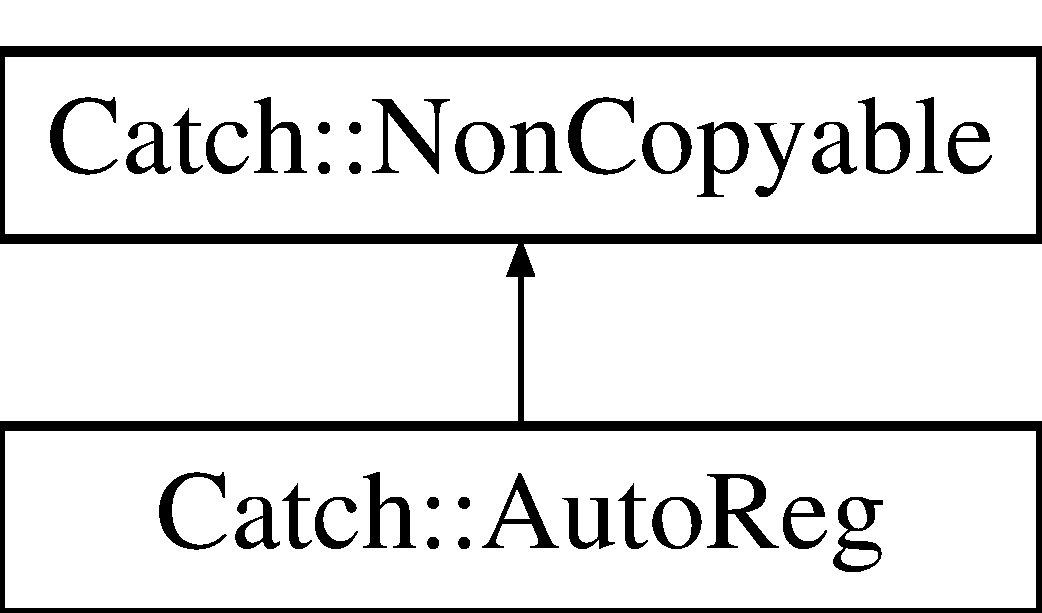
\includegraphics[height=2.000000cm]{struct_catch_1_1_auto_reg}
\end{center}
\end{figure}
\subsection*{Public Member Functions}
\begin{DoxyCompactItemize}
\item 
\mbox{\Hypertarget{struct_catch_1_1_auto_reg_a7eba02fb9d80b9896bf5a6517369af28}\label{struct_catch_1_1_auto_reg_a7eba02fb9d80b9896bf5a6517369af28}} 
{\bfseries Auto\+Reg} (\mbox{\hyperlink{struct_catch_1_1_i_test_invoker}{I\+Test\+Invoker}} $\ast$invoker, \mbox{\hyperlink{struct_catch_1_1_source_line_info}{Source\+Line\+Info}} const \&line\+Info, \mbox{\hyperlink{class_catch_1_1_string_ref}{String\+Ref}} const \&class\+Or\+Method, \mbox{\hyperlink{struct_catch_1_1_name_and_tags}{Name\+And\+Tags}} const \&name\+And\+Tags) noexcept
\end{DoxyCompactItemize}


The documentation for this struct was generated from the following file\+:\begin{DoxyCompactItemize}
\item 
catch.\+hpp\end{DoxyCompactItemize}

\hypertarget{class_catch_1_1_benchmark_looper}{}\section{Catch\+:\+:Benchmark\+Looper Class Reference}
\label{class_catch_1_1_benchmark_looper}\index{Catch\+::\+Benchmark\+Looper@{Catch\+::\+Benchmark\+Looper}}
\subsection*{Public Member Functions}
\begin{DoxyCompactItemize}
\item 
\mbox{\Hypertarget{class_catch_1_1_benchmark_looper_ab9ba6397306a70082f39e63a8a71bde6}\label{class_catch_1_1_benchmark_looper_ab9ba6397306a70082f39e63a8a71bde6}} 
{\bfseries Benchmark\+Looper} (\mbox{\hyperlink{class_catch_1_1_string_ref}{String\+Ref}} name)
\item 
\mbox{\Hypertarget{class_catch_1_1_benchmark_looper_a54da41bada9da038dc05faf41d746765}\label{class_catch_1_1_benchmark_looper_a54da41bada9da038dc05faf41d746765}} 
{\bfseries operator bool} ()
\item 
\mbox{\Hypertarget{class_catch_1_1_benchmark_looper_a210552aff5b19408637444d4bb35d59c}\label{class_catch_1_1_benchmark_looper_a210552aff5b19408637444d4bb35d59c}} 
void {\bfseries increment} ()
\item 
\mbox{\Hypertarget{class_catch_1_1_benchmark_looper_a0697d1b266112b110edf2025b82c4e77}\label{class_catch_1_1_benchmark_looper_a0697d1b266112b110edf2025b82c4e77}} 
void {\bfseries report\+Start} ()
\item 
\mbox{\Hypertarget{class_catch_1_1_benchmark_looper_a97bd944521f519b1593a5d1d2f9998fa}\label{class_catch_1_1_benchmark_looper_a97bd944521f519b1593a5d1d2f9998fa}} 
auto {\bfseries needs\+More\+Iterations} () -\/$>$ bool
\end{DoxyCompactItemize}


The documentation for this class was generated from the following file\+:\begin{DoxyCompactItemize}
\item 
catch.\+hpp\end{DoxyCompactItemize}

\hypertarget{class_bezier_surface_batch}{}\section{Bezier\+Surface\+Batch Class Reference}
\label{class_bezier_surface_batch}\index{Bezier\+Surface\+Batch@{Bezier\+Surface\+Batch}}
\subsection*{Public Member Functions}
\begin{DoxyCompactItemize}
\item 
\mbox{\Hypertarget{class_bezier_surface_batch_a548db6175908827d14b50829f1a3fecb}\label{class_bezier_surface_batch_a548db6175908827d14b50829f1a3fecb}} 
{\bfseries Bezier\+Surface\+Batch} (G\+Lfloat arrf\mbox{[}P\+S\+I\+ZE\mbox{]}\mbox{[}P\+S\+I\+ZE\mbox{]}\mbox{[}3\mbox{]})
\item 
\mbox{\Hypertarget{class_bezier_surface_batch_a178c5429aaa994e86e0684c561f01c57}\label{class_bezier_surface_batch_a178c5429aaa994e86e0684c561f01c57}} 
void {\bfseries create} ()
\item 
\mbox{\Hypertarget{class_bezier_surface_batch_a089ccb0b0a628c1d61086eec7eb9e4cd}\label{class_bezier_surface_batch_a089ccb0b0a628c1d61086eec7eb9e4cd}} 
void {\bfseries draw} ()
\item 
\mbox{\Hypertarget{class_bezier_surface_batch_acabb1d09583b705e194079f8eef45f5c}\label{class_bezier_surface_batch_acabb1d09583b705e194079f8eef45f5c}} 
void {\bfseries connect\+Curve} ()
\end{DoxyCompactItemize}


The documentation for this class was generated from the following file\+:\begin{DoxyCompactItemize}
\item 
Bezier\+Surface\+Batch.\+h\end{DoxyCompactItemize}

\hypertarget{class_catch_1_1_binary_expr}{}\section{Catch\+:\+:Binary\+Expr$<$ LhsT, RhsT $>$ Class Template Reference}
\label{class_catch_1_1_binary_expr}\index{Catch\+::\+Binary\+Expr$<$ Lhs\+T, Rhs\+T $>$@{Catch\+::\+Binary\+Expr$<$ Lhs\+T, Rhs\+T $>$}}
Inheritance diagram for Catch\+:\+:Binary\+Expr$<$ LhsT, RhsT $>$\+:\begin{figure}[H]
\begin{center}
\leavevmode
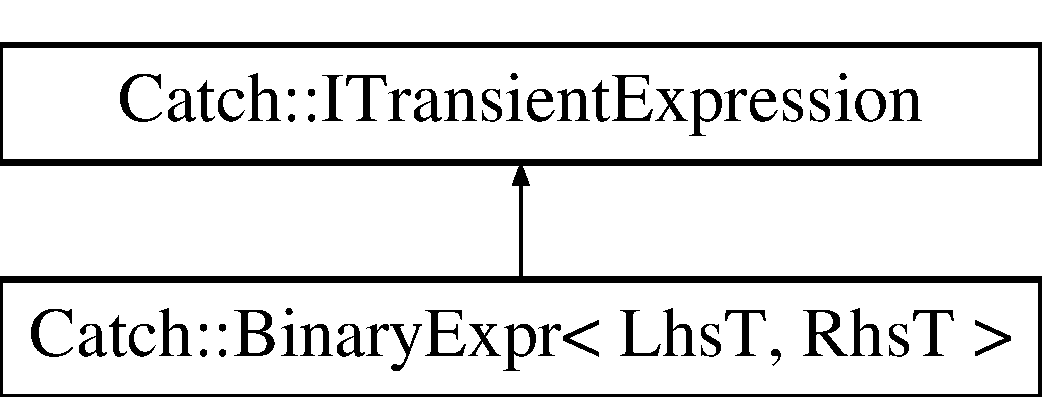
\includegraphics[height=2.000000cm]{class_catch_1_1_binary_expr}
\end{center}
\end{figure}
\subsection*{Public Member Functions}
\begin{DoxyCompactItemize}
\item 
\mbox{\Hypertarget{class_catch_1_1_binary_expr_a657d66346aef97a760c22776fe6008b6}\label{class_catch_1_1_binary_expr_a657d66346aef97a760c22776fe6008b6}} 
{\bfseries Binary\+Expr} (bool comparison\+Result, LhsT lhs, \mbox{\hyperlink{class_catch_1_1_string_ref}{String\+Ref}} op, RhsT rhs)
\end{DoxyCompactItemize}
\subsection*{Additional Inherited Members}


The documentation for this class was generated from the following file\+:\begin{DoxyCompactItemize}
\item 
catch.\+hpp\end{DoxyCompactItemize}

\hypertarget{class_b_s_t}{}\section{B\+ST$<$ Type $>$ Class Template Reference}
\label{class_b_s_t}\index{B\+S\+T$<$ Type $>$@{B\+S\+T$<$ Type $>$}}
\subsection*{Public Member Functions}
\begin{DoxyCompactItemize}
\item 
\mbox{\Hypertarget{class_b_s_t_af7a270543cf9a8578d2c76d97b095fc8}\label{class_b_s_t_af7a270543cf9a8578d2c76d97b095fc8}} 
void {\bfseries insert} (int n)
\item 
\mbox{\Hypertarget{class_b_s_t_a5a0f05ca244a5c4c2283374f14577e35}\label{class_b_s_t_a5a0f05ca244a5c4c2283374f14577e35}} 
void {\bfseries destroy\+Tree} (\mbox{\hyperlink{class_node}{Node}}$<$ Type $>$ $\ast$r)
\end{DoxyCompactItemize}
\subsection*{Public Attributes}
\begin{DoxyCompactItemize}
\item 
\mbox{\Hypertarget{class_b_s_t_af75b94874fc64895e1185cd4b657d2d2}\label{class_b_s_t_af75b94874fc64895e1185cd4b657d2d2}} 
\mbox{\hyperlink{class_node}{Node}}$<$ Type $>$ $\ast$ {\bfseries root}
\end{DoxyCompactItemize}


The documentation for this class was generated from the following file\+:\begin{DoxyCompactItemize}
\item 
B\+S\+T.\+h\end{DoxyCompactItemize}

\hypertarget{class_camera}{}\section{Camera Class Reference}
\label{class_camera}\index{Camera@{Camera}}
\subsection*{Public Member Functions}
\begin{DoxyCompactItemize}
\item 
\mbox{\Hypertarget{class_camera_a1af03aa27aafc84436078eb11e16c0e3}\label{class_camera_a1af03aa27aafc84436078eb11e16c0e3}} 
double {\bfseries getX} ()
\item 
\mbox{\Hypertarget{class_camera_a32713758e0f60a348681556d36e3d304}\label{class_camera_a32713758e0f60a348681556d36e3d304}} 
void {\bfseries set\+Theta} (double theta1)
\item 
\mbox{\Hypertarget{class_camera_a32491a1d934338e0e3f8303186bdb06e}\label{class_camera_a32491a1d934338e0e3f8303186bdb06e}} 
void {\bfseries set\+Alpha} (double alpha1)
\item 
\mbox{\Hypertarget{class_camera_abbc0b4141e683264260e325d239d7dcc}\label{class_camera_abbc0b4141e683264260e325d239d7dcc}} 
double {\bfseries get\+Radius} ()
\item 
\mbox{\Hypertarget{class_camera_a95c51b540e29bab525c14c43fbe5f6e4}\label{class_camera_a95c51b540e29bab525c14c43fbe5f6e4}} 
double {\bfseries get\+Alpha} ()
\item 
\mbox{\Hypertarget{class_camera_a07a610dd1015770d57b1370547154743}\label{class_camera_a07a610dd1015770d57b1370547154743}} 
double {\bfseries get\+Theta} ()
\item 
\mbox{\Hypertarget{class_camera_a1a99eaab2127fcc0af20e8e06e9a7eb0}\label{class_camera_a1a99eaab2127fcc0af20e8e06e9a7eb0}} 
double {\bfseries getY} ()
\item 
\mbox{\Hypertarget{class_camera_aead34062d4bdb7fca1241a480d3f563f}\label{class_camera_aead34062d4bdb7fca1241a480d3f563f}} 
double {\bfseries getZ} ()
\item 
\mbox{\Hypertarget{class_camera_acf2f00de2e99af1fcd9b5e770fce7ae3}\label{class_camera_acf2f00de2e99af1fcd9b5e770fce7ae3}} 
void {\bfseries move\+Right} ()
\item 
\mbox{\Hypertarget{class_camera_acbf35947eb5d887a76538e9525cf34a0}\label{class_camera_acbf35947eb5d887a76538e9525cf34a0}} 
void {\bfseries move\+Left} ()
\item 
\mbox{\Hypertarget{class_camera_aa6dc57f7ed60e5bfc106d48c7431c8c1}\label{class_camera_aa6dc57f7ed60e5bfc106d48c7431c8c1}} 
void {\bfseries move\+Up} ()
\item 
\mbox{\Hypertarget{class_camera_ab8c429b8547f3a106657ecd07dffc5bc}\label{class_camera_ab8c429b8547f3a106657ecd07dffc5bc}} 
void {\bfseries move\+Down} ()
\item 
\mbox{\Hypertarget{class_camera_a62d35e87b3eeac9463f43c17b65ef090}\label{class_camera_a62d35e87b3eeac9463f43c17b65ef090}} 
void {\bfseries zoom\+In} ()
\item 
\mbox{\Hypertarget{class_camera_aafc1d985053e11bd553b8a12540a562d}\label{class_camera_aafc1d985053e11bd553b8a12540a562d}} 
void {\bfseries zoom\+Out} ()
\item 
\mbox{\Hypertarget{class_camera_a6398913886565e782098849fcd3cffe5}\label{class_camera_a6398913886565e782098849fcd3cffe5}} 
void {\bfseries print} (double posx, double posy)
\end{DoxyCompactItemize}


The documentation for this class was generated from the following file\+:\begin{DoxyCompactItemize}
\item 
Camera.\+h\end{DoxyCompactItemize}

\hypertarget{class_catch_1_1_capturer}{}\section{Catch\+:\+:Capturer Class Reference}
\label{class_catch_1_1_capturer}\index{Catch\+::\+Capturer@{Catch\+::\+Capturer}}
\subsection*{Public Member Functions}
\begin{DoxyCompactItemize}
\item 
\mbox{\Hypertarget{class_catch_1_1_capturer_a86b0b27acc803a4e1310c10820f3038f}\label{class_catch_1_1_capturer_a86b0b27acc803a4e1310c10820f3038f}} 
{\bfseries Capturer} (\mbox{\hyperlink{class_catch_1_1_string_ref}{String\+Ref}} macro\+Name, \mbox{\hyperlink{struct_catch_1_1_source_line_info}{Source\+Line\+Info}} const \&line\+Info, Result\+Was\+::\+Of\+Type result\+Type, \mbox{\hyperlink{class_catch_1_1_string_ref}{String\+Ref}} names)
\item 
\mbox{\Hypertarget{class_catch_1_1_capturer_a45e14b9667dc9df7f5132507b322934c}\label{class_catch_1_1_capturer_a45e14b9667dc9df7f5132507b322934c}} 
void {\bfseries capture\+Value} (size\+\_\+t index, \mbox{\hyperlink{class_catch_1_1_string_ref}{String\+Ref}} value)
\item 
\mbox{\Hypertarget{class_catch_1_1_capturer_af0810e7f79b197648434d81b492a8c2b}\label{class_catch_1_1_capturer_af0810e7f79b197648434d81b492a8c2b}} 
{\footnotesize template$<$typename T $>$ }\\void {\bfseries capture\+Values} (size\+\_\+t index, T \&\&value)
\item 
\mbox{\Hypertarget{class_catch_1_1_capturer_a152c9083bfed800786673327b9c522ce}\label{class_catch_1_1_capturer_a152c9083bfed800786673327b9c522ce}} 
{\footnotesize template$<$typename T , typename... Ts$>$ }\\void {\bfseries capture\+Values} (size\+\_\+t index, T \&\&value, Ts \&\&... values)
\end{DoxyCompactItemize}


The documentation for this class was generated from the following file\+:\begin{DoxyCompactItemize}
\item 
catch.\+hpp\end{DoxyCompactItemize}

\hypertarget{struct_catch_1_1_matchers_1_1_std_string_1_1_cased_string}{}\section{Catch\+:\+:Matchers\+:\+:Std\+String\+:\+:Cased\+String Struct Reference}
\label{struct_catch_1_1_matchers_1_1_std_string_1_1_cased_string}\index{Catch\+::\+Matchers\+::\+Std\+String\+::\+Cased\+String@{Catch\+::\+Matchers\+::\+Std\+String\+::\+Cased\+String}}
\subsection*{Public Member Functions}
\begin{DoxyCompactItemize}
\item 
\mbox{\Hypertarget{struct_catch_1_1_matchers_1_1_std_string_1_1_cased_string_aa88bbc5acd2bff22351d8d4b1816b561}\label{struct_catch_1_1_matchers_1_1_std_string_1_1_cased_string_aa88bbc5acd2bff22351d8d4b1816b561}} 
{\bfseries Cased\+String} (std\+::string const \&str, Case\+Sensitive\+::\+Choice case\+Sensitivity)
\item 
\mbox{\Hypertarget{struct_catch_1_1_matchers_1_1_std_string_1_1_cased_string_a77639b1165c01f424ee0e96f53335010}\label{struct_catch_1_1_matchers_1_1_std_string_1_1_cased_string_a77639b1165c01f424ee0e96f53335010}} 
std\+::string {\bfseries adjust\+String} (std\+::string const \&str) const
\item 
\mbox{\Hypertarget{struct_catch_1_1_matchers_1_1_std_string_1_1_cased_string_a9759155344d696b2476d764a1d95fcc9}\label{struct_catch_1_1_matchers_1_1_std_string_1_1_cased_string_a9759155344d696b2476d764a1d95fcc9}} 
std\+::string {\bfseries case\+Sensitivity\+Suffix} () const
\end{DoxyCompactItemize}
\subsection*{Public Attributes}
\begin{DoxyCompactItemize}
\item 
\mbox{\Hypertarget{struct_catch_1_1_matchers_1_1_std_string_1_1_cased_string_ae1c2864c986941536a6e94cca0528f92}\label{struct_catch_1_1_matchers_1_1_std_string_1_1_cased_string_ae1c2864c986941536a6e94cca0528f92}} 
Case\+Sensitive\+::\+Choice {\bfseries m\+\_\+case\+Sensitivity}
\item 
\mbox{\Hypertarget{struct_catch_1_1_matchers_1_1_std_string_1_1_cased_string_ad05dbc99aba3c3c386d6b856b213f911}\label{struct_catch_1_1_matchers_1_1_std_string_1_1_cased_string_ad05dbc99aba3c3c386d6b856b213f911}} 
std\+::string {\bfseries m\+\_\+str}
\end{DoxyCompactItemize}


The documentation for this struct was generated from the following file\+:\begin{DoxyCompactItemize}
\item 
catch.\+hpp\end{DoxyCompactItemize}

\hypertarget{struct_catch_1_1_case_sensitive}{}\section{Catch\+:\+:Case\+Sensitive Struct Reference}
\label{struct_catch_1_1_case_sensitive}\index{Catch\+::\+Case\+Sensitive@{Catch\+::\+Case\+Sensitive}}
\subsection*{Public Types}
\begin{DoxyCompactItemize}
\item 
\mbox{\Hypertarget{struct_catch_1_1_case_sensitive_aad49d3aee2d97066642fffa919685c6a}\label{struct_catch_1_1_case_sensitive_aad49d3aee2d97066642fffa919685c6a}} 
enum {\bfseries Choice} \{ {\bfseries Yes}, 
{\bfseries No}
 \}
\end{DoxyCompactItemize}


The documentation for this struct was generated from the following file\+:\begin{DoxyCompactItemize}
\item 
catch.\+hpp\end{DoxyCompactItemize}

\hypertarget{struct_catch__global__namespace__dummy}{}\section{Catch\+\_\+global\+\_\+namespace\+\_\+dummy Struct Reference}
\label{struct_catch__global__namespace__dummy}\index{Catch\+\_\+global\+\_\+namespace\+\_\+dummy@{Catch\+\_\+global\+\_\+namespace\+\_\+dummy}}


The documentation for this struct was generated from the following file\+:\begin{DoxyCompactItemize}
\item 
catch.\+hpp\end{DoxyCompactItemize}

\hypertarget{class_checker_board}{}\section{Checker\+Board Class Reference}
\label{class_checker_board}\index{Checker\+Board@{Checker\+Board}}
\subsection*{Public Member Functions}
\begin{DoxyCompactItemize}
\item 
\mbox{\Hypertarget{class_checker_board_a25a56bec16a1dff98438f7a144bc5922}\label{class_checker_board_a25a56bec16a1dff98438f7a144bc5922}} 
{\bfseries Checker\+Board} (int width, int depth)
\item 
\mbox{\Hypertarget{class_checker_board_a4e07955cf06a9362ee3437795c3add88}\label{class_checker_board_a4e07955cf06a9362ee3437795c3add88}} 
double {\bfseries centerx} ()
\item 
\mbox{\Hypertarget{class_checker_board_afc3f580a5eb44d6922456ec8f8ce6c33}\label{class_checker_board_afc3f580a5eb44d6922456ec8f8ce6c33}} 
double {\bfseries centerz} ()
\item 
\mbox{\Hypertarget{class_checker_board_aab63f13410b7b7286fce32a1171027af}\label{class_checker_board_aab63f13410b7b7286fce32a1171027af}} 
void {\bfseries set\+Color} (G\+Lfloat c0\mbox{[}3\mbox{]}, G\+Lfloat c1\mbox{[}3\mbox{]})
\item 
\mbox{\Hypertarget{class_checker_board_ac9d20d984765bba78ecd5c0028980dd2}\label{class_checker_board_ac9d20d984765bba78ecd5c0028980dd2}} 
void {\bfseries create} ()
\item 
\mbox{\Hypertarget{class_checker_board_ac727ee4f4924e77702ee86e713ca90e6}\label{class_checker_board_ac727ee4f4924e77702ee86e713ca90e6}} 
void {\bfseries draw} ()
\end{DoxyCompactItemize}


The documentation for this class was generated from the following file\+:\begin{DoxyCompactItemize}
\item 
Checker\+Board.\+h\end{DoxyCompactItemize}

\hypertarget{class_circle}{}\section{Circle Class Reference}
\label{class_circle}\index{Circle@{Circle}}
\subsection*{Public Member Functions}
\begin{DoxyCompactItemize}
\item 
\mbox{\Hypertarget{class_circle_aac0b09b2ce1f2561c2937037d3a0e986}\label{class_circle_aac0b09b2ce1f2561c2937037d3a0e986}} 
{\bfseries Circle} (double cx, double cy)
\item 
\mbox{\Hypertarget{class_circle_a9da409203c0a3c27059663ec1ba5b84a}\label{class_circle_a9da409203c0a3c27059663ec1ba5b84a}} 
{\bfseries Circle} (double cx, double cy, int numc)
\item 
\mbox{\Hypertarget{class_circle_adc7fb01e543610dd34d127b5955b3b55}\label{class_circle_adc7fb01e543610dd34d127b5955b3b55}} 
{\bfseries Circle} (double cx, double cy, double radius, int numc)
\item 
\mbox{\Hypertarget{class_circle_a3a3f7166e7f629e44f9044b0e537eb22}\label{class_circle_a3a3f7166e7f629e44f9044b0e537eb22}} 
void {\bfseries draw} ()
\end{DoxyCompactItemize}


The documentation for this class was generated from the following file\+:\begin{DoxyCompactItemize}
\item 
Circle.\+h\end{DoxyCompactItemize}

\hypertarget{class_space_complex_1_1_complex}{}\section{Space\+Complex\+:\+:Complex Class Reference}
\label{class_space_complex_1_1_complex}\index{Space\+Complex\+::\+Complex@{Space\+Complex\+::\+Complex}}
\subsection*{Public Member Functions}
\begin{DoxyCompactItemize}
\item 
\mbox{\Hypertarget{class_space_complex_1_1_complex_a366b06ac1e3a9e6d41494fdc91ab8e0e}\label{class_space_complex_1_1_complex_a366b06ac1e3a9e6d41494fdc91ab8e0e}} 
{\bfseries Complex} (double x\+\_\+, double y\+\_\+)
\item 
\mbox{\Hypertarget{class_space_complex_1_1_complex_aea42c3fb8920152900502ef380b78225}\label{class_space_complex_1_1_complex_aea42c3fb8920152900502ef380b78225}} 
\mbox{\hyperlink{class_space_complex_1_1_complex}{Complex}} {\bfseries operator+} (\mbox{\hyperlink{class_space_complex_1_1_complex}{Complex}} \&c)
\item 
\mbox{\Hypertarget{class_space_complex_1_1_complex_a50f532f1f2a7126ec9eab75b338385c5}\label{class_space_complex_1_1_complex_a50f532f1f2a7126ec9eab75b338385c5}} 
\mbox{\hyperlink{class_space_complex_1_1_complex}{Complex}} {\bfseries operator-\/} (\mbox{\hyperlink{class_space_complex_1_1_complex}{Complex}} \&c)
\item 
\mbox{\Hypertarget{class_space_complex_1_1_complex_a8c0375773c39faf050f50d2979e5d31c}\label{class_space_complex_1_1_complex_a8c0375773c39faf050f50d2979e5d31c}} 
void {\bfseries print} ()
\end{DoxyCompactItemize}
\subsection*{Public Attributes}
\begin{DoxyCompactItemize}
\item 
\mbox{\Hypertarget{class_space_complex_1_1_complex_a9cda12c0bd13fe8b5193d85043e168a8}\label{class_space_complex_1_1_complex_a9cda12c0bd13fe8b5193d85043e168a8}} 
double {\bfseries x}
\item 
\mbox{\Hypertarget{class_space_complex_1_1_complex_a4297f745ee62818e6643e19e5dafbe0f}\label{class_space_complex_1_1_complex_a4297f745ee62818e6643e19e5dafbe0f}} 
double {\bfseries y}
\end{DoxyCompactItemize}


The documentation for this class was generated from the following file\+:\begin{DoxyCompactItemize}
\item 
Aron\+Lib.\+h\end{DoxyCompactItemize}

\hypertarget{struct_catch_1_1_matchers_1_1_vector_1_1_contains_element_matcher}{}\section{Catch\+:\+:Matchers\+:\+:Vector\+:\+:Contains\+Element\+Matcher$<$ T $>$ Struct Template Reference}
\label{struct_catch_1_1_matchers_1_1_vector_1_1_contains_element_matcher}\index{Catch\+::\+Matchers\+::\+Vector\+::\+Contains\+Element\+Matcher$<$ T $>$@{Catch\+::\+Matchers\+::\+Vector\+::\+Contains\+Element\+Matcher$<$ T $>$}}
Inheritance diagram for Catch\+:\+:Matchers\+:\+:Vector\+:\+:Contains\+Element\+Matcher$<$ T $>$\+:\begin{figure}[H]
\begin{center}
\leavevmode
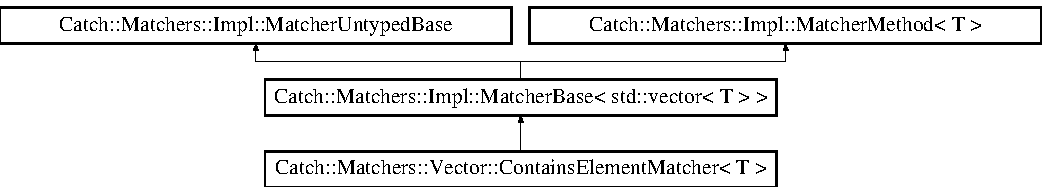
\includegraphics[height=2.514970cm]{struct_catch_1_1_matchers_1_1_vector_1_1_contains_element_matcher}
\end{center}
\end{figure}
\subsection*{Public Member Functions}
\begin{DoxyCompactItemize}
\item 
\mbox{\Hypertarget{struct_catch_1_1_matchers_1_1_vector_1_1_contains_element_matcher_a6a05740b5d3f89fac8de84ac0cff7b93}\label{struct_catch_1_1_matchers_1_1_vector_1_1_contains_element_matcher_a6a05740b5d3f89fac8de84ac0cff7b93}} 
{\bfseries Contains\+Element\+Matcher} (T const \&comparator)
\item 
\mbox{\Hypertarget{struct_catch_1_1_matchers_1_1_vector_1_1_contains_element_matcher_a6a4be6e5642e267433d370649beb0fac}\label{struct_catch_1_1_matchers_1_1_vector_1_1_contains_element_matcher_a6a4be6e5642e267433d370649beb0fac}} 
bool {\bfseries match} (std\+::vector$<$ T $>$ const \&v) const override
\item 
\mbox{\Hypertarget{struct_catch_1_1_matchers_1_1_vector_1_1_contains_element_matcher_aea3b674389a0afd82af6ba4b10f86ae6}\label{struct_catch_1_1_matchers_1_1_vector_1_1_contains_element_matcher_aea3b674389a0afd82af6ba4b10f86ae6}} 
std\+::string {\bfseries describe} () const override
\end{DoxyCompactItemize}
\subsection*{Public Attributes}
\begin{DoxyCompactItemize}
\item 
\mbox{\Hypertarget{struct_catch_1_1_matchers_1_1_vector_1_1_contains_element_matcher_ab7eada6c4bbce1d21b44773262f9cb23}\label{struct_catch_1_1_matchers_1_1_vector_1_1_contains_element_matcher_ab7eada6c4bbce1d21b44773262f9cb23}} 
T const  \& {\bfseries m\+\_\+comparator}
\end{DoxyCompactItemize}
\subsection*{Additional Inherited Members}


The documentation for this struct was generated from the following file\+:\begin{DoxyCompactItemize}
\item 
catch.\+hpp\end{DoxyCompactItemize}

\hypertarget{struct_catch_1_1_matchers_1_1_std_string_1_1_contains_matcher}{}\section{Catch\+:\+:Matchers\+:\+:Std\+String\+:\+:Contains\+Matcher Struct Reference}
\label{struct_catch_1_1_matchers_1_1_std_string_1_1_contains_matcher}\index{Catch\+::\+Matchers\+::\+Std\+String\+::\+Contains\+Matcher@{Catch\+::\+Matchers\+::\+Std\+String\+::\+Contains\+Matcher}}
Inheritance diagram for Catch\+:\+:Matchers\+:\+:Std\+String\+:\+:Contains\+Matcher\+:\begin{figure}[H]
\begin{center}
\leavevmode
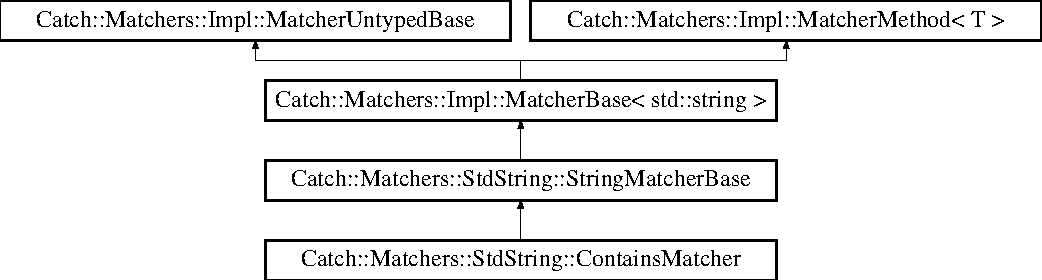
\includegraphics[height=3.758389cm]{struct_catch_1_1_matchers_1_1_std_string_1_1_contains_matcher}
\end{center}
\end{figure}
\subsection*{Public Member Functions}
\begin{DoxyCompactItemize}
\item 
\mbox{\Hypertarget{struct_catch_1_1_matchers_1_1_std_string_1_1_contains_matcher_acc892883c8409e34b28c9b39d4ef1fe3}\label{struct_catch_1_1_matchers_1_1_std_string_1_1_contains_matcher_acc892883c8409e34b28c9b39d4ef1fe3}} 
{\bfseries Contains\+Matcher} (\mbox{\hyperlink{struct_catch_1_1_matchers_1_1_std_string_1_1_cased_string}{Cased\+String}} const \&comparator)
\item 
\mbox{\Hypertarget{struct_catch_1_1_matchers_1_1_std_string_1_1_contains_matcher_a630628b234b037be83fe587081a80b53}\label{struct_catch_1_1_matchers_1_1_std_string_1_1_contains_matcher_a630628b234b037be83fe587081a80b53}} 
bool {\bfseries match} (std\+::string const \&source) const override
\end{DoxyCompactItemize}
\subsection*{Additional Inherited Members}


The documentation for this struct was generated from the following file\+:\begin{DoxyCompactItemize}
\item 
catch.\+hpp\end{DoxyCompactItemize}

\hypertarget{struct_catch_1_1_matchers_1_1_vector_1_1_contains_matcher}{}\section{Catch\+:\+:Matchers\+:\+:Vector\+:\+:Contains\+Matcher$<$ T $>$ Struct Template Reference}
\label{struct_catch_1_1_matchers_1_1_vector_1_1_contains_matcher}\index{Catch\+::\+Matchers\+::\+Vector\+::\+Contains\+Matcher$<$ T $>$@{Catch\+::\+Matchers\+::\+Vector\+::\+Contains\+Matcher$<$ T $>$}}
Inheritance diagram for Catch\+:\+:Matchers\+:\+:Vector\+:\+:Contains\+Matcher$<$ T $>$\+:\begin{figure}[H]
\begin{center}
\leavevmode
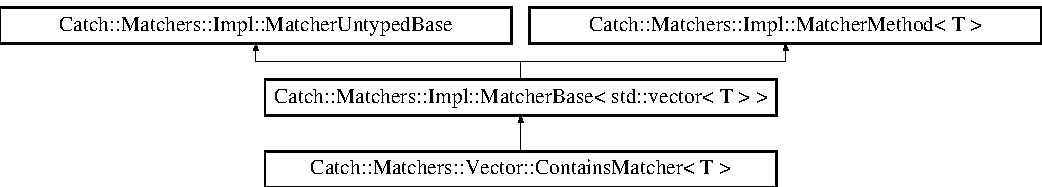
\includegraphics[height=2.514970cm]{struct_catch_1_1_matchers_1_1_vector_1_1_contains_matcher}
\end{center}
\end{figure}
\subsection*{Public Member Functions}
\begin{DoxyCompactItemize}
\item 
\mbox{\Hypertarget{struct_catch_1_1_matchers_1_1_vector_1_1_contains_matcher_ad8e92c8399be6dce75bb5702cdfab700}\label{struct_catch_1_1_matchers_1_1_vector_1_1_contains_matcher_ad8e92c8399be6dce75bb5702cdfab700}} 
{\bfseries Contains\+Matcher} (std\+::vector$<$ T $>$ const \&comparator)
\item 
\mbox{\Hypertarget{struct_catch_1_1_matchers_1_1_vector_1_1_contains_matcher_afd33467ae48a41a634572b41b053f67f}\label{struct_catch_1_1_matchers_1_1_vector_1_1_contains_matcher_afd33467ae48a41a634572b41b053f67f}} 
bool {\bfseries match} (std\+::vector$<$ T $>$ const \&v) const override
\item 
\mbox{\Hypertarget{struct_catch_1_1_matchers_1_1_vector_1_1_contains_matcher_abe6a9ea3d6506c9a1f75ff524f35832e}\label{struct_catch_1_1_matchers_1_1_vector_1_1_contains_matcher_abe6a9ea3d6506c9a1f75ff524f35832e}} 
std\+::string {\bfseries describe} () const override
\end{DoxyCompactItemize}
\subsection*{Public Attributes}
\begin{DoxyCompactItemize}
\item 
\mbox{\Hypertarget{struct_catch_1_1_matchers_1_1_vector_1_1_contains_matcher_a83d051166e4ed0d535219ad6ee99abb2}\label{struct_catch_1_1_matchers_1_1_vector_1_1_contains_matcher_a83d051166e4ed0d535219ad6ee99abb2}} 
std\+::vector$<$ T $>$ const  \& {\bfseries m\+\_\+comparator}
\end{DoxyCompactItemize}
\subsection*{Additional Inherited Members}


The documentation for this struct was generated from the following file\+:\begin{DoxyCompactItemize}
\item 
catch.\+hpp\end{DoxyCompactItemize}

\hypertarget{class_coordinate}{}\section{Coordinate Class Reference}
\label{class_coordinate}\index{Coordinate@{Coordinate}}
\subsection*{Public Member Functions}
\begin{DoxyCompactItemize}
\item 
\mbox{\Hypertarget{class_coordinate_a165954d2c9ca5d4b387f47da8dc22d73}\label{class_coordinate_a165954d2c9ca5d4b387f47da8dc22d73}} 
{\bfseries Coordinate} (double width)
\item 
\mbox{\Hypertarget{class_coordinate_a3ba09b433fc40588f9982f4f432c0fce}\label{class_coordinate_a3ba09b433fc40588f9982f4f432c0fce}} 
{\bfseries Coordinate} (double width, double radius)
\item 
\mbox{\Hypertarget{class_coordinate_a5833a110d4e166e1d95721588fa58bde}\label{class_coordinate_a5833a110d4e166e1d95721588fa58bde}} 
{\bfseries Coordinate} (double width, double radius, int nstep)
\item 
\mbox{\Hypertarget{class_coordinate_ade43612d120d6a3c9c32f05e4a31c523}\label{class_coordinate_ade43612d120d6a3c9c32f05e4a31c523}} 
void {\bfseries draw} ()
\end{DoxyCompactItemize}


The documentation for this class was generated from the following file\+:\begin{DoxyCompactItemize}
\item 
Coordinate.\+h\end{DoxyCompactItemize}

\hypertarget{struct_catch_1_1_counts}{}\section{Catch\+:\+:Counts Struct Reference}
\label{struct_catch_1_1_counts}\index{Catch\+::\+Counts@{Catch\+::\+Counts}}
\subsection*{Public Member Functions}
\begin{DoxyCompactItemize}
\item 
\mbox{\Hypertarget{struct_catch_1_1_counts_aaa10666f559057e3e860d2a5a6fae4c4}\label{struct_catch_1_1_counts_aaa10666f559057e3e860d2a5a6fae4c4}} 
\mbox{\hyperlink{struct_catch_1_1_counts}{Counts}} {\bfseries operator-\/} (\mbox{\hyperlink{struct_catch_1_1_counts}{Counts}} const \&other) const
\item 
\mbox{\Hypertarget{struct_catch_1_1_counts_a322a89475cd2cc039140ef371e973677}\label{struct_catch_1_1_counts_a322a89475cd2cc039140ef371e973677}} 
\mbox{\hyperlink{struct_catch_1_1_counts}{Counts}} \& {\bfseries operator+=} (\mbox{\hyperlink{struct_catch_1_1_counts}{Counts}} const \&other)
\item 
\mbox{\Hypertarget{struct_catch_1_1_counts_a94f969c09cf52d1339c085c9603cd1d3}\label{struct_catch_1_1_counts_a94f969c09cf52d1339c085c9603cd1d3}} 
std\+::size\+\_\+t {\bfseries total} () const
\item 
\mbox{\Hypertarget{struct_catch_1_1_counts_a84999490e0ecaa3de5e121bf48eda1b3}\label{struct_catch_1_1_counts_a84999490e0ecaa3de5e121bf48eda1b3}} 
bool {\bfseries all\+Passed} () const
\item 
\mbox{\Hypertarget{struct_catch_1_1_counts_a33bd996e016030155b99fe1c51c08991}\label{struct_catch_1_1_counts_a33bd996e016030155b99fe1c51c08991}} 
bool {\bfseries all\+Ok} () const
\end{DoxyCompactItemize}
\subsection*{Public Attributes}
\begin{DoxyCompactItemize}
\item 
\mbox{\Hypertarget{struct_catch_1_1_counts_ad28daaf3de28006400208b6dd0c631e6}\label{struct_catch_1_1_counts_ad28daaf3de28006400208b6dd0c631e6}} 
std\+::size\+\_\+t {\bfseries passed} = 0
\item 
\mbox{\Hypertarget{struct_catch_1_1_counts_a19982a3817a3bc2c07f0290e71f497a3}\label{struct_catch_1_1_counts_a19982a3817a3bc2c07f0290e71f497a3}} 
std\+::size\+\_\+t {\bfseries failed} = 0
\item 
\mbox{\Hypertarget{struct_catch_1_1_counts_ac090973a2ff51394cd452718e75c073e}\label{struct_catch_1_1_counts_ac090973a2ff51394cd452718e75c073e}} 
std\+::size\+\_\+t {\bfseries failed\+But\+Ok} = 0
\end{DoxyCompactItemize}


The documentation for this struct was generated from the following file\+:\begin{DoxyCompactItemize}
\item 
catch.\+hpp\end{DoxyCompactItemize}

\hypertarget{class_cube}{}\section{Cube Class Reference}
\label{class_cube}\index{Cube@{Cube}}
\subsection*{Public Member Functions}
\begin{DoxyCompactItemize}
\item 
\mbox{\Hypertarget{class_cube_a49aeb021ee94d8281944170ba293491a}\label{class_cube_a49aeb021ee94d8281944170ba293491a}} 
{\bfseries Cube} (float x1, float y1, float z1, float r1=1.\+0)
\item 
\mbox{\Hypertarget{class_cube_ab26b72a81376fd5dc4fcc7f0b715b087}\label{class_cube_ab26b72a81376fd5dc4fcc7f0b715b087}} 
void {\bfseries draw} ()
\end{DoxyCompactItemize}
\subsection*{Public Attributes}
\begin{DoxyCompactItemize}
\item 
\mbox{\Hypertarget{class_cube_a3e0558b8c87b7a13cd7182255cbc190b}\label{class_cube_a3e0558b8c87b7a13cd7182255cbc190b}} 
float {\bfseries x} = 1.\+0f
\item 
\mbox{\Hypertarget{class_cube_a5710bde4446d58489fdf4eb4fc091c43}\label{class_cube_a5710bde4446d58489fdf4eb4fc091c43}} 
float {\bfseries y}
\item 
\mbox{\Hypertarget{class_cube_a5470969e64ec3adb5299ac7a0362df02}\label{class_cube_a5470969e64ec3adb5299ac7a0362df02}} 
float {\bfseries z}
\item 
\mbox{\Hypertarget{class_cube_a8a4af26ee6d9ead878aea2b34d92eb2e}\label{class_cube_a8a4af26ee6d9ead878aea2b34d92eb2e}} 
float {\bfseries r}
\item 
G\+Lfloat {\bfseries vertices} \mbox{[}108\mbox{]}
\end{DoxyCompactItemize}


\subsection{Member Data Documentation}
\mbox{\Hypertarget{class_cube_a85348252cbcb13296e1786d0368ccf09}\label{class_cube_a85348252cbcb13296e1786d0368ccf09}} 
\index{Cube@{Cube}!vertices@{vertices}}
\index{vertices@{vertices}!Cube@{Cube}}
\subsubsection{\texorpdfstring{vertices}{vertices}}
{\footnotesize\ttfamily G\+Lfloat Cube\+::vertices\mbox{[}108\mbox{]}}

{\bfseries Initial value\+:}
\begin{DoxyCode}
= \{ 1, 1, 1,  -1, 1, 1,  -1,-1, 1,      
                       -1,-1, 1,   1,-1, 1,   1, 1, 1,      

                        1, 1, 1,   1,-1, 1,   1,-1,-1,      
                        1,-1,-1,   1, 1,-1,   1, 1, 1,      

                        1, 1, 1,   1, 1,-1,  -1, 1,-1,      
                       -1, 1,-1,  -1, 1, 1,   1, 1, 1,      

                       -1, 1, 1,  -1, 1,-1,  -1,-1,-1,      
                       -1,-1,-1,  -1,-1, 1,  -1, 1, 1,      

                       -1,-1,-1,   1,-1,-1,   1,-1, 1,      
                        1,-1, 1,  -1,-1, 1,  -1,-1,-1,      

                        1,-1,-1,  -1,-1,-1,  -1, 1,-1,      
                       -1, 1,-1,   1, 1,-1,   1,-1,-1 \}
\end{DoxyCode}


The documentation for this class was generated from the following file\+:\begin{DoxyCompactItemize}
\item 
Cube.\+h\end{DoxyCompactItemize}

\hypertarget{class_curve}{}\section{Curve Class Reference}
\label{class_curve}\index{Curve@{Curve}}
\subsection*{Public Member Functions}
\begin{DoxyCompactItemize}
\item 
\mbox{\Hypertarget{class_curve_a02f2af392d6b58dea2670cbda7507258}\label{class_curve_a02f2af392d6b58dea2670cbda7507258}} 
{\bfseries Curve} (\mbox{\hyperlink{class_vector3}{Vector3}} p0, \mbox{\hyperlink{class_vector3}{Vector3}} p1, \mbox{\hyperlink{class_vector3}{Vector3}} p2, int level=3)
\item 
\mbox{\Hypertarget{class_curve_abf50fa354857985ce18f9753e452331e}\label{class_curve_abf50fa354857985ce18f9753e452331e}} 
{\bfseries Curve} (\mbox{\hyperlink{class_vector3}{Vector3}} p0, \mbox{\hyperlink{class_vector3}{Vector3}} p1, \mbox{\hyperlink{class_vector3}{Vector3}} p2, \mbox{\hyperlink{class_vector3}{Vector3}} p3, int level=3)
\item 
\mbox{\Hypertarget{class_curve_a32c7bd32d4acebaef0517c2c1d64f49d}\label{class_curve_a32c7bd32d4acebaef0517c2c1d64f49d}} 
void {\bfseries draw} ()
\item 
\mbox{\Hypertarget{class_curve_a27c5022ae8df5e634999aab65f708621}\label{class_curve_a27c5022ae8df5e634999aab65f708621}} 
void {\bfseries set\+Color} (G\+Lfloat color\mbox{[}3\mbox{]})
\end{DoxyCompactItemize}
\subsection*{Public Attributes}
\begin{DoxyCompactItemize}
\item 
\mbox{\Hypertarget{class_curve_ae2321eec1b936ebd263d50008170b58f}\label{class_curve_ae2321eec1b936ebd263d50008170b58f}} 
\mbox{\hyperlink{class_d_d_linked_list}{D\+D\+Linked\+List}}$<$ \mbox{\hyperlink{class_vector3}{Vector3}} $>$ $\ast$ {\bfseries ddl} = new \mbox{\hyperlink{class_d_d_linked_list}{D\+D\+Linked\+List}}$<$\mbox{\hyperlink{class_vector3}{Vector3}}$>$()
\end{DoxyCompactItemize}


The documentation for this class was generated from the following file\+:\begin{DoxyCompactItemize}
\item 
Curve.\+h\end{DoxyCompactItemize}

\hypertarget{class_cylinder}{}\section{Cylinder Class Reference}
\label{class_cylinder}\index{Cylinder@{Cylinder}}
\subsection*{Public Member Functions}
\begin{DoxyCompactItemize}
\item 
\mbox{\Hypertarget{class_cylinder_a9a1e51eb9eada3c894a2fccc9a6dcf5a}\label{class_cylinder_a9a1e51eb9eada3c894a2fccc9a6dcf5a}} 
{\bfseries Cylinder} (double cx, double cy, double depth)
\item 
\mbox{\Hypertarget{class_cylinder_a5e660df9688ae3675b7e368da0cc1dd2}\label{class_cylinder_a5e660df9688ae3675b7e368da0cc1dd2}} 
{\bfseries Cylinder} (double cx, double cy, double depth, double radius, int numc)
\item 
\mbox{\Hypertarget{class_cylinder_a44a1bd72e100d72e8419c3b2f589e2bf}\label{class_cylinder_a44a1bd72e100d72e8419c3b2f589e2bf}} 
{\bfseries Cylinder} (double cx, double cy, double radius, int numc)
\item 
\mbox{\Hypertarget{class_cylinder_a1140cf9d4d125eba323a5067b2bc6e7c}\label{class_cylinder_a1140cf9d4d125eba323a5067b2bc6e7c}} 
void {\bfseries set\+Color} (G\+Lfloat c0\mbox{[}3\mbox{]}, G\+Lfloat c1\mbox{[}3\mbox{]})
\item 
\mbox{\Hypertarget{class_cylinder_af7fc0a5e40d1a84563f94ee5de1e2838}\label{class_cylinder_af7fc0a5e40d1a84563f94ee5de1e2838}} 
void {\bfseries lighting} ()
\item 
\mbox{\Hypertarget{class_cylinder_a89992ad8e5aff4f40a5f496076ff4d52}\label{class_cylinder_a89992ad8e5aff4f40a5f496076ff4d52}} 
void {\bfseries draw} ()
\end{DoxyCompactItemize}


The documentation for this class was generated from the following file\+:\begin{DoxyCompactItemize}
\item 
Cylinder.\+h\end{DoxyCompactItemize}

\hypertarget{class_d_d_linked_list}{}\section{D\+D\+Linked\+List$<$ Type $>$ Class Template Reference}
\label{class_d_d_linked_list}\index{D\+D\+Linked\+List$<$ Type $>$@{D\+D\+Linked\+List$<$ Type $>$}}
\subsection*{Public Member Functions}
\begin{DoxyCompactItemize}
\item 
\mbox{\Hypertarget{class_d_d_linked_list_ac71de6448e246a49682db52b4f9db49f}\label{class_d_d_linked_list_ac71de6448e246a49682db52b4f9db49f}} 
int {\bfseries count} ()
\item 
\mbox{\Hypertarget{class_d_d_linked_list_a545e4d81e9d86b80dfda3c0dd5589ff7}\label{class_d_d_linked_list_a545e4d81e9d86b80dfda3c0dd5589ff7}} 
void {\bfseries append} (Type data)
\item 
\mbox{\Hypertarget{class_d_d_linked_list_a39627249e8fd24249e152967e1988dd5}\label{class_d_d_linked_list_a39627249e8fd24249e152967e1988dd5}} 
void {\bfseries append} (\mbox{\hyperlink{class_node}{Node}}$<$ Type $>$ $\ast$node)
\item 
\mbox{\Hypertarget{class_d_d_linked_list_abe5ea588678c869a4bb511f9f10622a3}\label{class_d_d_linked_list_abe5ea588678c869a4bb511f9f10622a3}} 
void {\bfseries remove} (Type data)
\item 
\mbox{\Hypertarget{class_d_d_linked_list_afcc8260230b0814e03b1918d6fb452e2}\label{class_d_d_linked_list_afcc8260230b0814e03b1918d6fb452e2}} 
void {\bfseries remove} (\mbox{\hyperlink{class_node}{Node}}$<$ Type $>$ $\ast$remove)
\end{DoxyCompactItemize}
\subsection*{Public Attributes}
\begin{DoxyCompactItemize}
\item 
\mbox{\Hypertarget{class_d_d_linked_list_a0749288fb8a7c4059cdd8b53759386ec}\label{class_d_d_linked_list_a0749288fb8a7c4059cdd8b53759386ec}} 
\mbox{\hyperlink{class_node}{Node}}$<$ Type $>$ $\ast$ {\bfseries head}
\item 
\mbox{\Hypertarget{class_d_d_linked_list_a7f319683d77c3324cc0b53f901baedbd}\label{class_d_d_linked_list_a7f319683d77c3324cc0b53f901baedbd}} 
\mbox{\hyperlink{class_node}{Node}}$<$ Type $>$ $\ast$ {\bfseries tail}
\end{DoxyCompactItemize}


The documentation for this class was generated from the following file\+:\begin{DoxyCompactItemize}
\item 
D\+D\+Linked\+List.\+h\end{DoxyCompactItemize}

\hypertarget{struct_catch_1_1_decomposer}{}\section{Catch\+:\+:Decomposer Struct Reference}
\label{struct_catch_1_1_decomposer}\index{Catch\+::\+Decomposer@{Catch\+::\+Decomposer}}
\subsection*{Public Member Functions}
\begin{DoxyCompactItemize}
\item 
\mbox{\Hypertarget{struct_catch_1_1_decomposer_a20b5b8c0e2ff0328a019ae1a8deca03a}\label{struct_catch_1_1_decomposer_a20b5b8c0e2ff0328a019ae1a8deca03a}} 
{\footnotesize template$<$typename T $>$ }\\auto {\bfseries operator$<$=} (T const \&lhs) -\/$>$ \mbox{\hyperlink{class_catch_1_1_expr_lhs}{Expr\+Lhs}}$<$ T const \&$>$
\item 
\mbox{\Hypertarget{struct_catch_1_1_decomposer_aac129b94903ae1339d5709049d83613b}\label{struct_catch_1_1_decomposer_aac129b94903ae1339d5709049d83613b}} 
auto {\bfseries operator$<$=} (bool value) -\/$>$ \mbox{\hyperlink{class_catch_1_1_expr_lhs}{Expr\+Lhs}}$<$ bool $>$
\end{DoxyCompactItemize}


The documentation for this struct was generated from the following file\+:\begin{DoxyCompactItemize}
\item 
catch.\+hpp\end{DoxyCompactItemize}

\hypertarget{class_draw_quad}{}\section{Draw\+Quad Class Reference}
\label{class_draw_quad}\index{Draw\+Quad@{Draw\+Quad}}
\subsection*{Public Member Functions}
\begin{DoxyCompactItemize}
\item 
\mbox{\Hypertarget{class_draw_quad_a24c571610de1cf6ab05da5b86db13f7b}\label{class_draw_quad_a24c571610de1cf6ab05da5b86db13f7b}} 
void {\bfseries draw} ()
\end{DoxyCompactItemize}


The documentation for this class was generated from the following file\+:\begin{DoxyCompactItemize}
\item 
Draw\+Quad.\+h\end{DoxyCompactItemize}

\hypertarget{struct_catch_1_1_matchers_1_1_std_string_1_1_ends_with_matcher}{}\section{Catch\+:\+:Matchers\+:\+:Std\+String\+:\+:Ends\+With\+Matcher Struct Reference}
\label{struct_catch_1_1_matchers_1_1_std_string_1_1_ends_with_matcher}\index{Catch\+::\+Matchers\+::\+Std\+String\+::\+Ends\+With\+Matcher@{Catch\+::\+Matchers\+::\+Std\+String\+::\+Ends\+With\+Matcher}}
Inheritance diagram for Catch\+:\+:Matchers\+:\+:Std\+String\+:\+:Ends\+With\+Matcher\+:\begin{figure}[H]
\begin{center}
\leavevmode
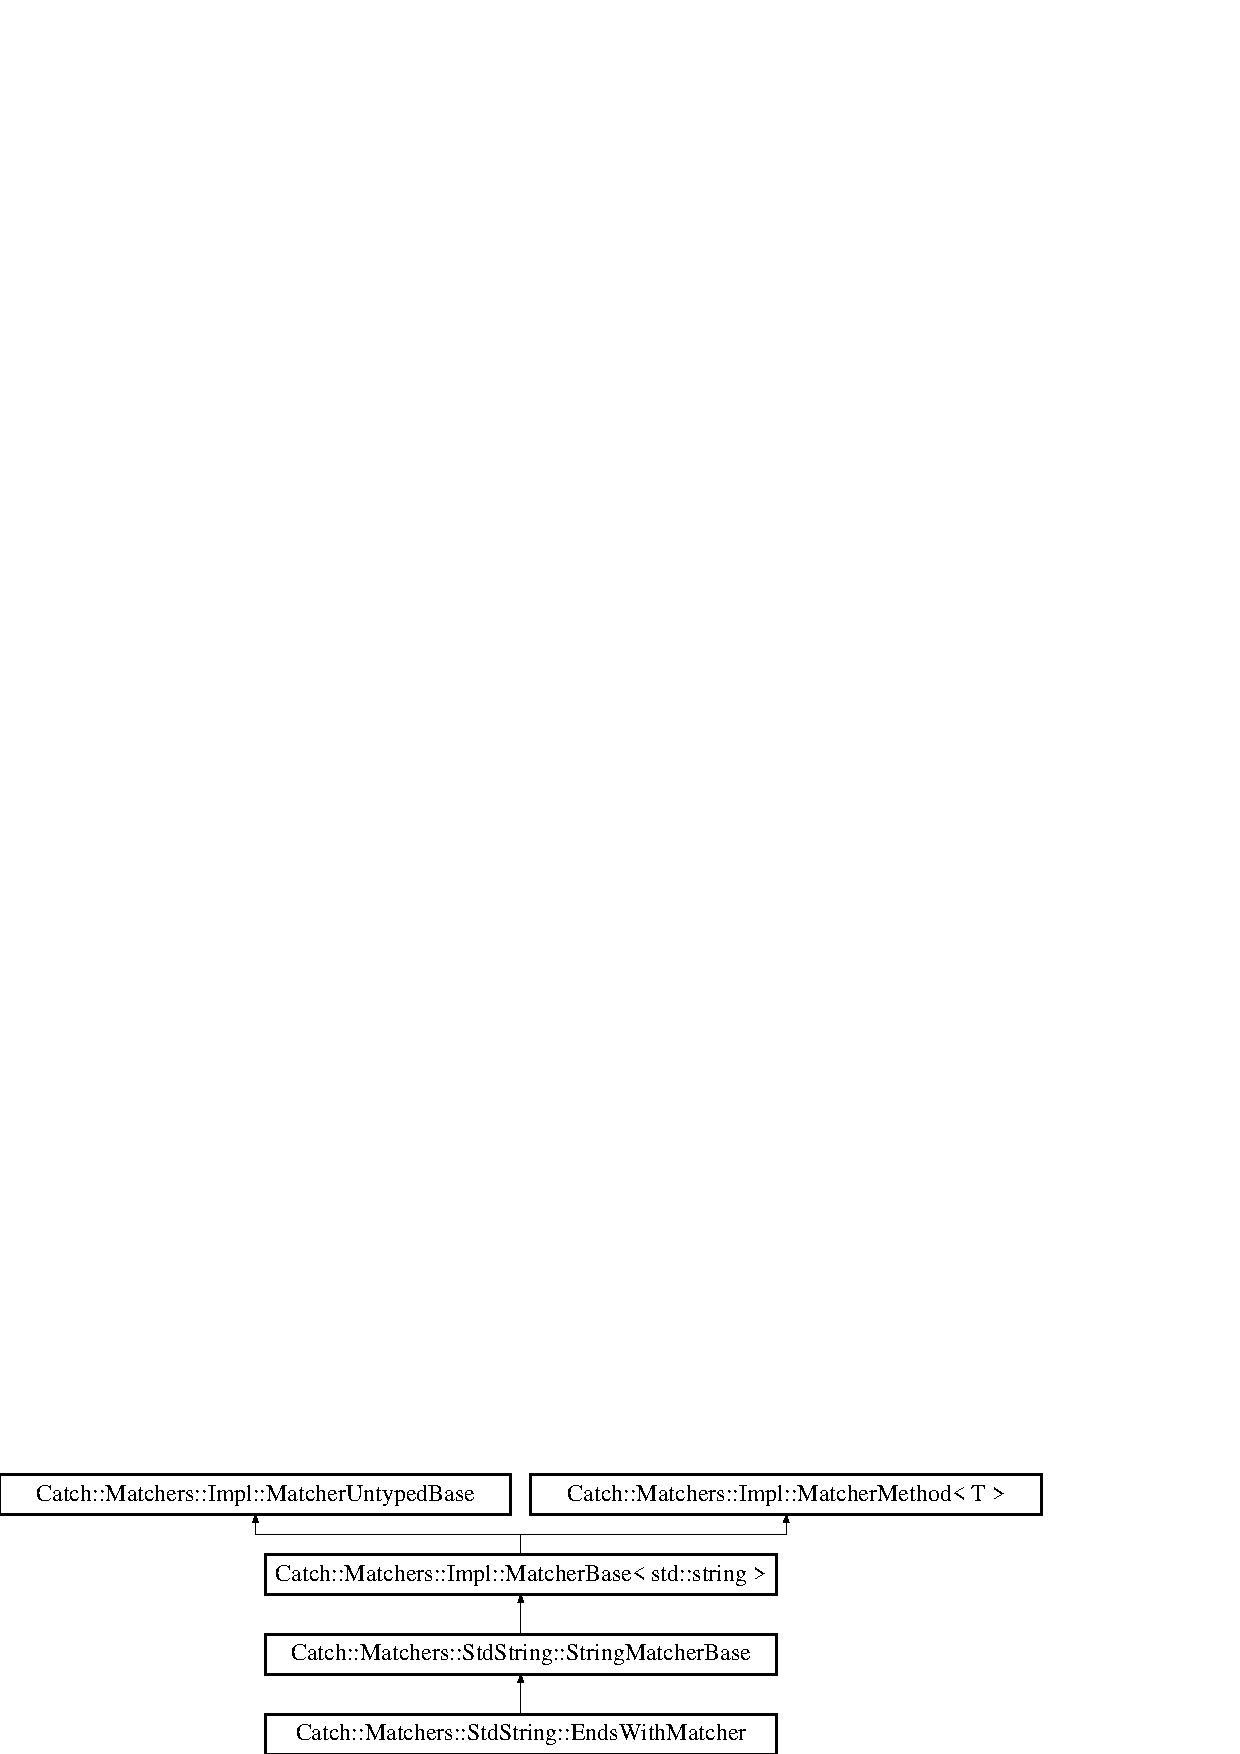
\includegraphics[height=3.758389cm]{struct_catch_1_1_matchers_1_1_std_string_1_1_ends_with_matcher}
\end{center}
\end{figure}
\subsection*{Public Member Functions}
\begin{DoxyCompactItemize}
\item 
\mbox{\Hypertarget{struct_catch_1_1_matchers_1_1_std_string_1_1_ends_with_matcher_aa5ec700b4629562f74f362080accfd7b}\label{struct_catch_1_1_matchers_1_1_std_string_1_1_ends_with_matcher_aa5ec700b4629562f74f362080accfd7b}} 
{\bfseries Ends\+With\+Matcher} (\mbox{\hyperlink{struct_catch_1_1_matchers_1_1_std_string_1_1_cased_string}{Cased\+String}} const \&comparator)
\item 
\mbox{\Hypertarget{struct_catch_1_1_matchers_1_1_std_string_1_1_ends_with_matcher_aca2741fa57374a2a98d2a84ac3e13a6d}\label{struct_catch_1_1_matchers_1_1_std_string_1_1_ends_with_matcher_aca2741fa57374a2a98d2a84ac3e13a6d}} 
bool {\bfseries match} (std\+::string const \&source) const override
\end{DoxyCompactItemize}
\subsection*{Additional Inherited Members}


The documentation for this struct was generated from the following file\+:\begin{DoxyCompactItemize}
\item 
catch.\+hpp\end{DoxyCompactItemize}

\hypertarget{struct_catch_1_1_matchers_1_1_std_string_1_1_equals_matcher}{}\section{Catch\+:\+:Matchers\+:\+:Std\+String\+:\+:Equals\+Matcher Struct Reference}
\label{struct_catch_1_1_matchers_1_1_std_string_1_1_equals_matcher}\index{Catch\+::\+Matchers\+::\+Std\+String\+::\+Equals\+Matcher@{Catch\+::\+Matchers\+::\+Std\+String\+::\+Equals\+Matcher}}
Inheritance diagram for Catch\+:\+:Matchers\+:\+:Std\+String\+:\+:Equals\+Matcher\+:\begin{figure}[H]
\begin{center}
\leavevmode
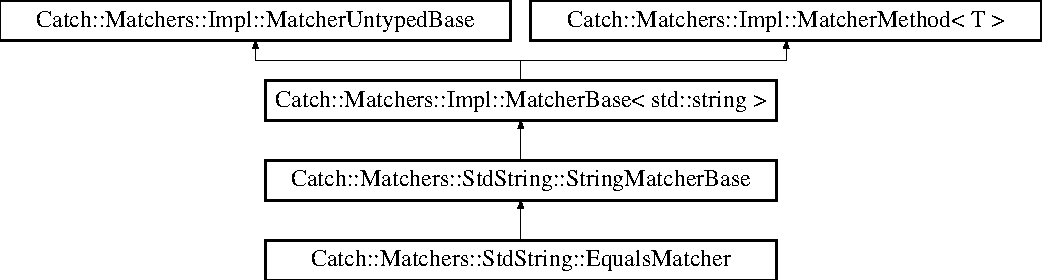
\includegraphics[height=3.758389cm]{struct_catch_1_1_matchers_1_1_std_string_1_1_equals_matcher}
\end{center}
\end{figure}
\subsection*{Public Member Functions}
\begin{DoxyCompactItemize}
\item 
\mbox{\Hypertarget{struct_catch_1_1_matchers_1_1_std_string_1_1_equals_matcher_ab740f1fb2310e9fe3fed5134d4c7e4c8}\label{struct_catch_1_1_matchers_1_1_std_string_1_1_equals_matcher_ab740f1fb2310e9fe3fed5134d4c7e4c8}} 
{\bfseries Equals\+Matcher} (\mbox{\hyperlink{struct_catch_1_1_matchers_1_1_std_string_1_1_cased_string}{Cased\+String}} const \&comparator)
\item 
\mbox{\Hypertarget{struct_catch_1_1_matchers_1_1_std_string_1_1_equals_matcher_a0bb9d64693f7bb1ef7441062d219f21a}\label{struct_catch_1_1_matchers_1_1_std_string_1_1_equals_matcher_a0bb9d64693f7bb1ef7441062d219f21a}} 
bool {\bfseries match} (std\+::string const \&source) const override
\end{DoxyCompactItemize}
\subsection*{Additional Inherited Members}


The documentation for this struct was generated from the following file\+:\begin{DoxyCompactItemize}
\item 
catch.\+hpp\end{DoxyCompactItemize}

\hypertarget{struct_catch_1_1_matchers_1_1_vector_1_1_equals_matcher}{}\section{Catch\+:\+:Matchers\+:\+:Vector\+:\+:Equals\+Matcher$<$ T $>$ Struct Template Reference}
\label{struct_catch_1_1_matchers_1_1_vector_1_1_equals_matcher}\index{Catch\+::\+Matchers\+::\+Vector\+::\+Equals\+Matcher$<$ T $>$@{Catch\+::\+Matchers\+::\+Vector\+::\+Equals\+Matcher$<$ T $>$}}
Inheritance diagram for Catch\+:\+:Matchers\+:\+:Vector\+:\+:Equals\+Matcher$<$ T $>$\+:\begin{figure}[H]
\begin{center}
\leavevmode
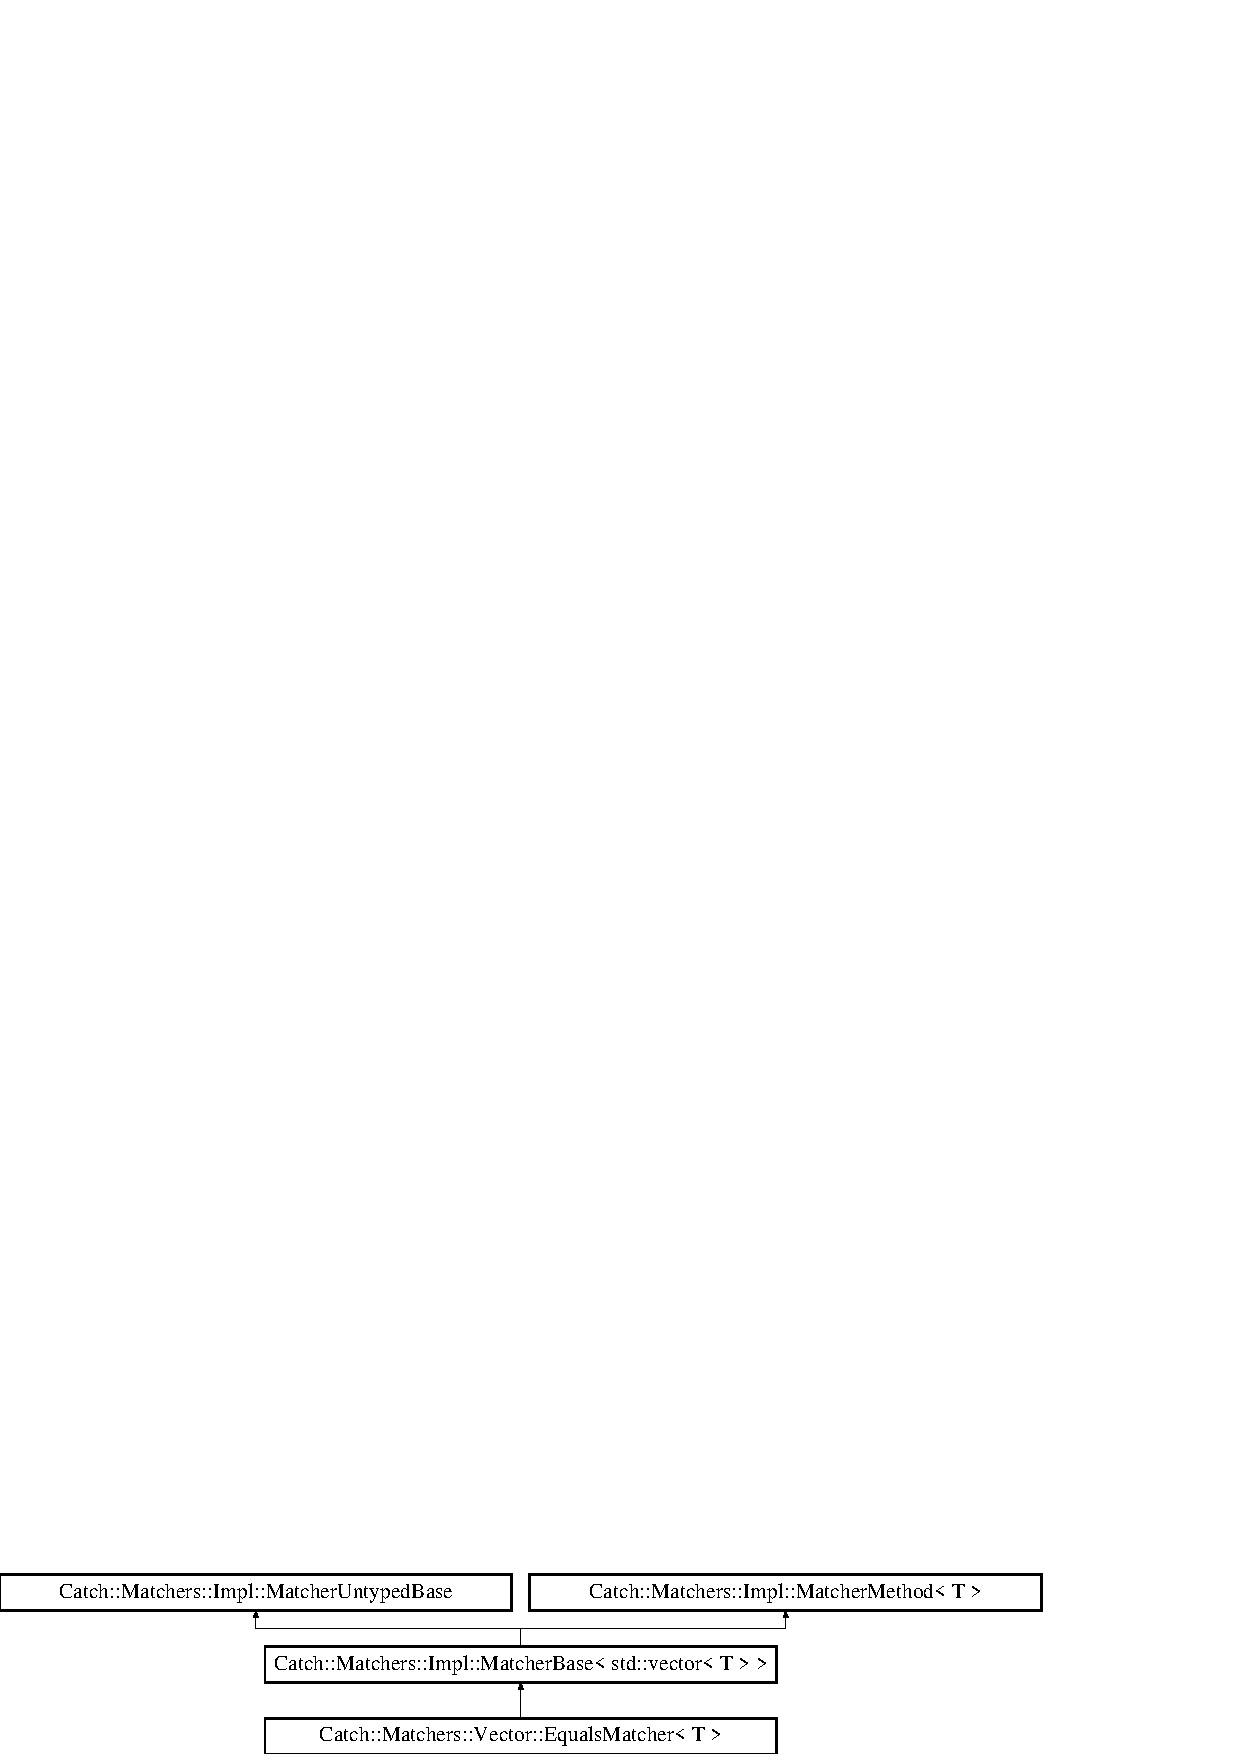
\includegraphics[height=2.514970cm]{struct_catch_1_1_matchers_1_1_vector_1_1_equals_matcher}
\end{center}
\end{figure}
\subsection*{Public Member Functions}
\begin{DoxyCompactItemize}
\item 
\mbox{\Hypertarget{struct_catch_1_1_matchers_1_1_vector_1_1_equals_matcher_a3846c47780d1991dcfe87aefded98008}\label{struct_catch_1_1_matchers_1_1_vector_1_1_equals_matcher_a3846c47780d1991dcfe87aefded98008}} 
{\bfseries Equals\+Matcher} (std\+::vector$<$ T $>$ const \&comparator)
\item 
\mbox{\Hypertarget{struct_catch_1_1_matchers_1_1_vector_1_1_equals_matcher_a2d96cca58a44151fddc5257eda3305da}\label{struct_catch_1_1_matchers_1_1_vector_1_1_equals_matcher_a2d96cca58a44151fddc5257eda3305da}} 
bool {\bfseries match} (std\+::vector$<$ T $>$ const \&v) const override
\item 
\mbox{\Hypertarget{struct_catch_1_1_matchers_1_1_vector_1_1_equals_matcher_a36b5f7ecada4081d6c65bebe8ddea6f4}\label{struct_catch_1_1_matchers_1_1_vector_1_1_equals_matcher_a36b5f7ecada4081d6c65bebe8ddea6f4}} 
std\+::string {\bfseries describe} () const override
\end{DoxyCompactItemize}
\subsection*{Public Attributes}
\begin{DoxyCompactItemize}
\item 
\mbox{\Hypertarget{struct_catch_1_1_matchers_1_1_vector_1_1_equals_matcher_a56f7aa6f110a12b1b9aeb0cabbc9d755}\label{struct_catch_1_1_matchers_1_1_vector_1_1_equals_matcher_a56f7aa6f110a12b1b9aeb0cabbc9d755}} 
std\+::vector$<$ T $>$ const  \& {\bfseries m\+\_\+comparator}
\end{DoxyCompactItemize}
\subsection*{Additional Inherited Members}


The documentation for this struct was generated from the following file\+:\begin{DoxyCompactItemize}
\item 
catch.\+hpp\end{DoxyCompactItemize}

\hypertarget{class_catch_1_1_exception_translator_registrar}{}\section{Catch\+:\+:Exception\+Translator\+Registrar Class Reference}
\label{class_catch_1_1_exception_translator_registrar}\index{Catch\+::\+Exception\+Translator\+Registrar@{Catch\+::\+Exception\+Translator\+Registrar}}
\subsection*{Public Member Functions}
\begin{DoxyCompactItemize}
\item 
\mbox{\Hypertarget{class_catch_1_1_exception_translator_registrar_aa73229de911f26b1df6c6c87c4d9e04e}\label{class_catch_1_1_exception_translator_registrar_aa73229de911f26b1df6c6c87c4d9e04e}} 
{\footnotesize template$<$typename T $>$ }\\{\bfseries Exception\+Translator\+Registrar} (std\+::string($\ast$translate\+Function)(T \&))
\end{DoxyCompactItemize}


The documentation for this class was generated from the following file\+:\begin{DoxyCompactItemize}
\item 
catch.\+hpp\end{DoxyCompactItemize}

\hypertarget{class_catch_1_1_expr_lhs}{}\section{Catch\+:\+:Expr\+Lhs$<$ LhsT $>$ Class Template Reference}
\label{class_catch_1_1_expr_lhs}\index{Catch\+::\+Expr\+Lhs$<$ Lhs\+T $>$@{Catch\+::\+Expr\+Lhs$<$ Lhs\+T $>$}}
\subsection*{Public Member Functions}
\begin{DoxyCompactItemize}
\item 
\mbox{\Hypertarget{class_catch_1_1_expr_lhs_ad22c6af1a7d6993240624d299714a479}\label{class_catch_1_1_expr_lhs_ad22c6af1a7d6993240624d299714a479}} 
{\bfseries Expr\+Lhs} (LhsT lhs)
\item 
\mbox{\Hypertarget{class_catch_1_1_expr_lhs_a3068adff1dbbaeec62ffc368d4d6cc4d}\label{class_catch_1_1_expr_lhs_a3068adff1dbbaeec62ffc368d4d6cc4d}} 
{\footnotesize template$<$typename RhsT $>$ }\\auto {\bfseries operator==} (RhsT const \&rhs) -\/$>$ \mbox{\hyperlink{class_catch_1_1_binary_expr}{Binary\+Expr}}$<$ LhsT, RhsT const \&$>$ const
\item 
\mbox{\Hypertarget{class_catch_1_1_expr_lhs_ab707a84abdffbdc35962a495e238d393}\label{class_catch_1_1_expr_lhs_ab707a84abdffbdc35962a495e238d393}} 
auto {\bfseries operator==} (bool rhs) -\/$>$ \mbox{\hyperlink{class_catch_1_1_binary_expr}{Binary\+Expr}}$<$ LhsT, bool $>$ const
\item 
\mbox{\Hypertarget{class_catch_1_1_expr_lhs_a5e10eab8aed53dd000b89d8fd7754437}\label{class_catch_1_1_expr_lhs_a5e10eab8aed53dd000b89d8fd7754437}} 
{\footnotesize template$<$typename RhsT $>$ }\\auto {\bfseries operator!=} (RhsT const \&rhs) -\/$>$ \mbox{\hyperlink{class_catch_1_1_binary_expr}{Binary\+Expr}}$<$ LhsT, RhsT const \&$>$ const
\item 
\mbox{\Hypertarget{class_catch_1_1_expr_lhs_a60eca847201d057d8a8b7222c69b619c}\label{class_catch_1_1_expr_lhs_a60eca847201d057d8a8b7222c69b619c}} 
auto {\bfseries operator!=} (bool rhs) -\/$>$ \mbox{\hyperlink{class_catch_1_1_binary_expr}{Binary\+Expr}}$<$ LhsT, bool $>$ const
\item 
\mbox{\Hypertarget{class_catch_1_1_expr_lhs_a23cb0cd983a1ac9c3df5160542199b83}\label{class_catch_1_1_expr_lhs_a23cb0cd983a1ac9c3df5160542199b83}} 
{\footnotesize template$<$typename RhsT $>$ }\\auto {\bfseries operator$>$} (RhsT const \&rhs) -\/$>$ \mbox{\hyperlink{class_catch_1_1_binary_expr}{Binary\+Expr}}$<$ LhsT, RhsT const \&$>$ const
\item 
\mbox{\Hypertarget{class_catch_1_1_expr_lhs_a55284221df2edb3542e765c87b5691b9}\label{class_catch_1_1_expr_lhs_a55284221df2edb3542e765c87b5691b9}} 
{\footnotesize template$<$typename RhsT $>$ }\\auto {\bfseries operator$<$} (RhsT const \&rhs) -\/$>$ \mbox{\hyperlink{class_catch_1_1_binary_expr}{Binary\+Expr}}$<$ LhsT, RhsT const \&$>$ const
\item 
\mbox{\Hypertarget{class_catch_1_1_expr_lhs_aff594ae5b957105c517a6257d2e730f0}\label{class_catch_1_1_expr_lhs_aff594ae5b957105c517a6257d2e730f0}} 
{\footnotesize template$<$typename RhsT $>$ }\\auto {\bfseries operator$>$=} (RhsT const \&rhs) -\/$>$ \mbox{\hyperlink{class_catch_1_1_binary_expr}{Binary\+Expr}}$<$ LhsT, RhsT const \&$>$ const
\item 
\mbox{\Hypertarget{class_catch_1_1_expr_lhs_a6bd8a22c1a7fe2f66d71d7196f20af4f}\label{class_catch_1_1_expr_lhs_a6bd8a22c1a7fe2f66d71d7196f20af4f}} 
{\footnotesize template$<$typename RhsT $>$ }\\auto {\bfseries operator$<$=} (RhsT const \&rhs) -\/$>$ \mbox{\hyperlink{class_catch_1_1_binary_expr}{Binary\+Expr}}$<$ LhsT, RhsT const \&$>$ const
\item 
\mbox{\Hypertarget{class_catch_1_1_expr_lhs_ab68bd6d5d3ae21b7fba9010150fba95d}\label{class_catch_1_1_expr_lhs_ab68bd6d5d3ae21b7fba9010150fba95d}} 
auto {\bfseries make\+Unary\+Expr} () const -\/$>$ \mbox{\hyperlink{class_catch_1_1_unary_expr}{Unary\+Expr}}$<$ LhsT $>$
\end{DoxyCompactItemize}


The documentation for this class was generated from the following file\+:\begin{DoxyCompactItemize}
\item 
catch.\+hpp\end{DoxyCompactItemize}

\hypertarget{class_catch_1_1_generators_1_1_fixed_values_generator}{}\section{Catch\+:\+:Generators\+:\+:Fixed\+Values\+Generator$<$ T $>$ Class Template Reference}
\label{class_catch_1_1_generators_1_1_fixed_values_generator}\index{Catch\+::\+Generators\+::\+Fixed\+Values\+Generator$<$ T $>$@{Catch\+::\+Generators\+::\+Fixed\+Values\+Generator$<$ T $>$}}
Inheritance diagram for Catch\+:\+:Generators\+:\+:Fixed\+Values\+Generator$<$ T $>$\+:\begin{figure}[H]
\begin{center}
\leavevmode
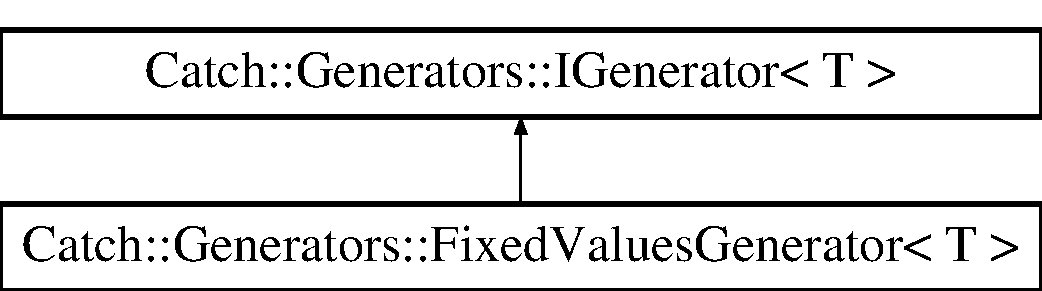
\includegraphics[height=2.000000cm]{class_catch_1_1_generators_1_1_fixed_values_generator}
\end{center}
\end{figure}
\subsection*{Public Member Functions}
\begin{DoxyCompactItemize}
\item 
\mbox{\Hypertarget{class_catch_1_1_generators_1_1_fixed_values_generator_a6e9f473655413c1cb15f079890f06b86}\label{class_catch_1_1_generators_1_1_fixed_values_generator_a6e9f473655413c1cb15f079890f06b86}} 
{\bfseries Fixed\+Values\+Generator} (std\+::initializer\+\_\+list$<$ T $>$ values)
\item 
\mbox{\Hypertarget{class_catch_1_1_generators_1_1_fixed_values_generator_a3ed654a5860c170dbe7b01487b83253d}\label{class_catch_1_1_generators_1_1_fixed_values_generator_a3ed654a5860c170dbe7b01487b83253d}} 
auto {\bfseries get} (size\+\_\+t index) const -\/$>$ T override
\end{DoxyCompactItemize}


The documentation for this class was generated from the following file\+:\begin{DoxyCompactItemize}
\item 
catch.\+hpp\end{DoxyCompactItemize}

\hypertarget{class_catch_1_1_generators_1_1_generator}{}\section{Catch\+:\+:Generators\+:\+:Generator$<$ T $>$ Class Template Reference}
\label{class_catch_1_1_generators_1_1_generator}\index{Catch\+::\+Generators\+::\+Generator$<$ T $>$@{Catch\+::\+Generators\+::\+Generator$<$ T $>$}}
\subsection*{Public Member Functions}
\begin{DoxyCompactItemize}
\item 
\mbox{\Hypertarget{class_catch_1_1_generators_1_1_generator_a3d992b33c5c1abb7370065c6ae10388f}\label{class_catch_1_1_generators_1_1_generator_a3d992b33c5c1abb7370065c6ae10388f}} 
{\bfseries Generator} (size\+\_\+t size, std\+::unique\+\_\+ptr$<$ \mbox{\hyperlink{struct_catch_1_1_generators_1_1_i_generator}{I\+Generator}}$<$ T $>$$>$ generator)
\item 
\mbox{\Hypertarget{class_catch_1_1_generators_1_1_generator_a4ebea9a7448f8f374bc7cff5d7b63041}\label{class_catch_1_1_generators_1_1_generator_a4ebea9a7448f8f374bc7cff5d7b63041}} 
auto {\bfseries size} () const -\/$>$ size\+\_\+t
\item 
\mbox{\Hypertarget{class_catch_1_1_generators_1_1_generator_ad8835935e962baaf1fab6c6dcac83865}\label{class_catch_1_1_generators_1_1_generator_ad8835935e962baaf1fab6c6dcac83865}} 
auto {\bfseries operator\mbox{[}$\,$\mbox{]}} (size\+\_\+t index) const -\/$>$ T
\end{DoxyCompactItemize}


The documentation for this class was generated from the following file\+:\begin{DoxyCompactItemize}
\item 
catch.\+hpp\end{DoxyCompactItemize}

\hypertarget{class_catch_1_1_generators_1_1_generator_base}{}\section{Catch\+:\+:Generators\+:\+:Generator\+Base Class Reference}
\label{class_catch_1_1_generators_1_1_generator_base}\index{Catch\+::\+Generators\+::\+Generator\+Base@{Catch\+::\+Generators\+::\+Generator\+Base}}
Inheritance diagram for Catch\+:\+:Generators\+:\+:Generator\+Base\+:\begin{figure}[H]
\begin{center}
\leavevmode
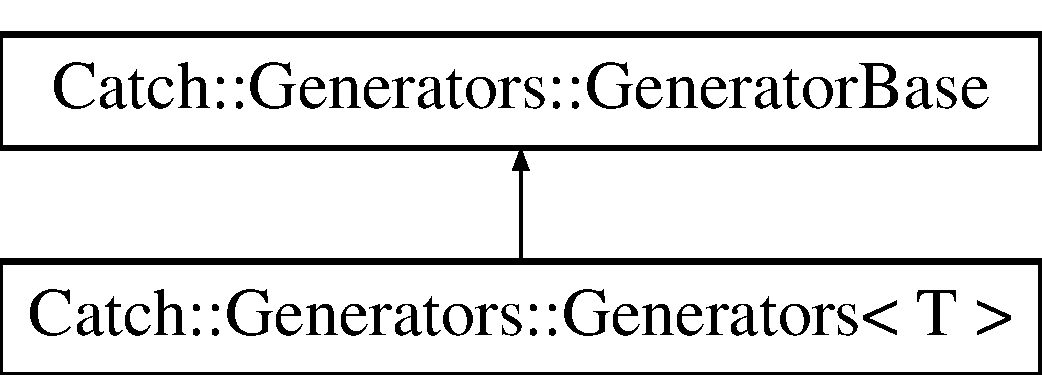
\includegraphics[height=2.000000cm]{class_catch_1_1_generators_1_1_generator_base}
\end{center}
\end{figure}
\subsection*{Public Member Functions}
\begin{DoxyCompactItemize}
\item 
\mbox{\Hypertarget{class_catch_1_1_generators_1_1_generator_base_ab003974d458a14acfb48f79e7e8abe21}\label{class_catch_1_1_generators_1_1_generator_base_ab003974d458a14acfb48f79e7e8abe21}} 
{\bfseries Generator\+Base} (size\+\_\+t size)
\item 
\mbox{\Hypertarget{class_catch_1_1_generators_1_1_generator_base_a2fb4a5c153f3fdc2708245b40751b487}\label{class_catch_1_1_generators_1_1_generator_base_a2fb4a5c153f3fdc2708245b40751b487}} 
auto {\bfseries size} () const -\/$>$ size\+\_\+t
\end{DoxyCompactItemize}
\subsection*{Protected Attributes}
\begin{DoxyCompactItemize}
\item 
\mbox{\Hypertarget{class_catch_1_1_generators_1_1_generator_base_ac6ab90adfdda9401e2ea03db5b2dfc6a}\label{class_catch_1_1_generators_1_1_generator_base_ac6ab90adfdda9401e2ea03db5b2dfc6a}} 
size\+\_\+t {\bfseries m\+\_\+size} = 0
\end{DoxyCompactItemize}


The documentation for this class was generated from the following file\+:\begin{DoxyCompactItemize}
\item 
catch.\+hpp\end{DoxyCompactItemize}

\hypertarget{class_catch_1_1_generators_1_1_generator_randomiser}{}\section{Catch\+:\+:Generators\+:\+:Generator\+Randomiser$<$ T $>$ Class Template Reference}
\label{class_catch_1_1_generators_1_1_generator_randomiser}\index{Catch\+::\+Generators\+::\+Generator\+Randomiser$<$ T $>$@{Catch\+::\+Generators\+::\+Generator\+Randomiser$<$ T $>$}}
Inheritance diagram for Catch\+:\+:Generators\+:\+:Generator\+Randomiser$<$ T $>$\+:\begin{figure}[H]
\begin{center}
\leavevmode
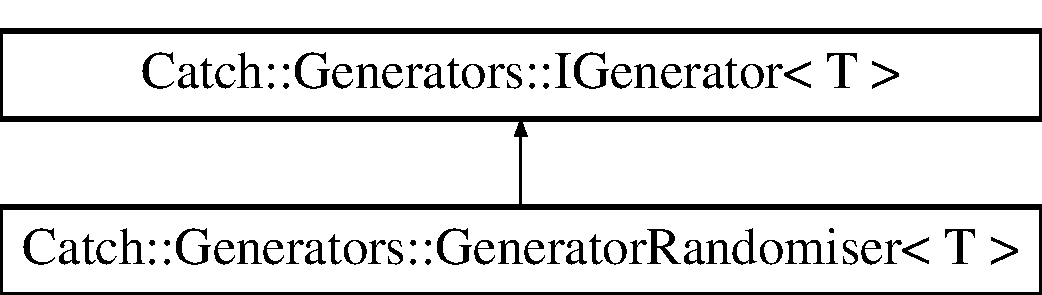
\includegraphics[height=2.000000cm]{class_catch_1_1_generators_1_1_generator_randomiser}
\end{center}
\end{figure}
\subsection*{Public Member Functions}
\begin{DoxyCompactItemize}
\item 
\mbox{\Hypertarget{class_catch_1_1_generators_1_1_generator_randomiser_aba3234a2885baff107766814d10c2efc}\label{class_catch_1_1_generators_1_1_generator_randomiser_aba3234a2885baff107766814d10c2efc}} 
{\bfseries Generator\+Randomiser} (\mbox{\hyperlink{class_catch_1_1_generators_1_1_generator}{Generator}}$<$ T $>$ \&\&base\+Generator, size\+\_\+t number\+Of\+Items)
\item 
\mbox{\Hypertarget{class_catch_1_1_generators_1_1_generator_randomiser_a4ad5de15865727bdaa638863e0969ab4}\label{class_catch_1_1_generators_1_1_generator_randomiser_a4ad5de15865727bdaa638863e0969ab4}} 
auto {\bfseries get} (size\+\_\+t index) const -\/$>$ T override
\end{DoxyCompactItemize}


The documentation for this class was generated from the following file\+:\begin{DoxyCompactItemize}
\item 
catch.\+hpp\end{DoxyCompactItemize}

\hypertarget{struct_catch_1_1_generators_1_1_generators}{}\section{Catch\+:\+:Generators\+:\+:Generators$<$ T $>$ Struct Template Reference}
\label{struct_catch_1_1_generators_1_1_generators}\index{Catch\+::\+Generators\+::\+Generators$<$ T $>$@{Catch\+::\+Generators\+::\+Generators$<$ T $>$}}
Inheritance diagram for Catch\+:\+:Generators\+:\+:Generators$<$ T $>$\+:\begin{figure}[H]
\begin{center}
\leavevmode
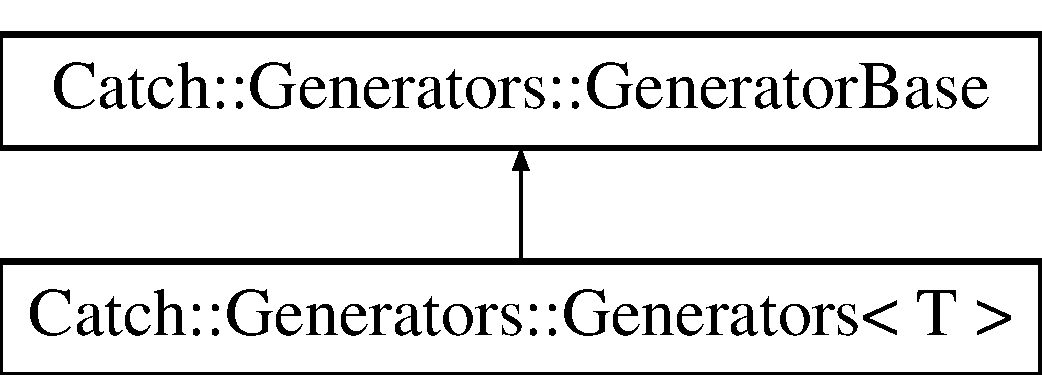
\includegraphics[height=2.000000cm]{struct_catch_1_1_generators_1_1_generators}
\end{center}
\end{figure}
\subsection*{Public Types}
\begin{DoxyCompactItemize}
\item 
\mbox{\Hypertarget{struct_catch_1_1_generators_1_1_generators_aab27f98a577b49532b2ca7556a84286b}\label{struct_catch_1_1_generators_1_1_generators_aab27f98a577b49532b2ca7556a84286b}} 
using {\bfseries type} = T
\end{DoxyCompactItemize}
\subsection*{Public Member Functions}
\begin{DoxyCompactItemize}
\item 
\mbox{\Hypertarget{struct_catch_1_1_generators_1_1_generators_ad708036fa5a9bf0cd1520ce111bc851d}\label{struct_catch_1_1_generators_1_1_generators_ad708036fa5a9bf0cd1520ce111bc851d}} 
void {\bfseries populate} (T \&\&val)
\item 
\mbox{\Hypertarget{struct_catch_1_1_generators_1_1_generators_a8ff8b7dda734d1808b644fefc67f4c98}\label{struct_catch_1_1_generators_1_1_generators_a8ff8b7dda734d1808b644fefc67f4c98}} 
{\footnotesize template$<$typename U $>$ }\\void {\bfseries populate} (U \&\&val)
\item 
\mbox{\Hypertarget{struct_catch_1_1_generators_1_1_generators_a2155cad48ab03c362483e200d957eefc}\label{struct_catch_1_1_generators_1_1_generators_a2155cad48ab03c362483e200d957eefc}} 
void {\bfseries populate} (\mbox{\hyperlink{class_catch_1_1_generators_1_1_generator}{Generator}}$<$ T $>$ \&\&generator)
\item 
\mbox{\Hypertarget{struct_catch_1_1_generators_1_1_generators_a4b9680ee28e48e4dc4c4538b5510e649}\label{struct_catch_1_1_generators_1_1_generators_a4b9680ee28e48e4dc4c4538b5510e649}} 
{\footnotesize template$<$typename U , typename... Gs$>$ }\\void {\bfseries populate} (U \&\&value\+Or\+Generator, Gs... more\+Generators)
\item 
\mbox{\Hypertarget{struct_catch_1_1_generators_1_1_generators_a1812ebb7d0146d63e3a005e93831afa2}\label{struct_catch_1_1_generators_1_1_generators_a1812ebb7d0146d63e3a005e93831afa2}} 
auto {\bfseries operator\mbox{[}$\,$\mbox{]}} (size\+\_\+t index) const -\/$>$ T
\end{DoxyCompactItemize}
\subsection*{Public Attributes}
\begin{DoxyCompactItemize}
\item 
\mbox{\Hypertarget{struct_catch_1_1_generators_1_1_generators_a49f1d0e8851a4726bb9981edffe094fa}\label{struct_catch_1_1_generators_1_1_generators_a49f1d0e8851a4726bb9981edffe094fa}} 
std\+::vector$<$ \mbox{\hyperlink{class_catch_1_1_generators_1_1_generator}{Generator}}$<$ T $>$ $>$ {\bfseries m\+\_\+generators}
\end{DoxyCompactItemize}
\subsection*{Additional Inherited Members}


The documentation for this struct was generated from the following file\+:\begin{DoxyCompactItemize}
\item 
catch.\+hpp\end{DoxyCompactItemize}

\hypertarget{struct_catch_1_1_i_exception_translator}{}\section{Catch\+:\+:I\+Exception\+Translator Struct Reference}
\label{struct_catch_1_1_i_exception_translator}\index{Catch\+::\+I\+Exception\+Translator@{Catch\+::\+I\+Exception\+Translator}}
\subsection*{Public Member Functions}
\begin{DoxyCompactItemize}
\item 
\mbox{\Hypertarget{struct_catch_1_1_i_exception_translator_a2a554b96ed5ed411e7c796b6b42837a5}\label{struct_catch_1_1_i_exception_translator_a2a554b96ed5ed411e7c796b6b42837a5}} 
virtual std\+::string {\bfseries translate} (Exception\+Translators\+::const\+\_\+iterator it, Exception\+Translators\+::const\+\_\+iterator it\+End) const =0
\end{DoxyCompactItemize}


The documentation for this struct was generated from the following file\+:\begin{DoxyCompactItemize}
\item 
catch.\+hpp\end{DoxyCompactItemize}

\hypertarget{struct_catch_1_1_i_exception_translator_registry}{}\section{Catch\+:\+:I\+Exception\+Translator\+Registry Struct Reference}
\label{struct_catch_1_1_i_exception_translator_registry}\index{Catch\+::\+I\+Exception\+Translator\+Registry@{Catch\+::\+I\+Exception\+Translator\+Registry}}
\subsection*{Public Member Functions}
\begin{DoxyCompactItemize}
\item 
\mbox{\Hypertarget{struct_catch_1_1_i_exception_translator_registry_af76ae8c331a17f2a94c9720bc0d686bb}\label{struct_catch_1_1_i_exception_translator_registry_af76ae8c331a17f2a94c9720bc0d686bb}} 
virtual std\+::string {\bfseries translate\+Active\+Exception} () const =0
\end{DoxyCompactItemize}


The documentation for this struct was generated from the following file\+:\begin{DoxyCompactItemize}
\item 
catch.\+hpp\end{DoxyCompactItemize}

\hypertarget{struct_catch_1_1_generators_1_1_i_generator}{}\section{Catch\+:\+:Generators\+:\+:I\+Generator$<$ T $>$ Struct Template Reference}
\label{struct_catch_1_1_generators_1_1_i_generator}\index{Catch\+::\+Generators\+::\+I\+Generator$<$ T $>$@{Catch\+::\+Generators\+::\+I\+Generator$<$ T $>$}}
Inheritance diagram for Catch\+:\+:Generators\+:\+:I\+Generator$<$ T $>$\+:\begin{figure}[H]
\begin{center}
\leavevmode
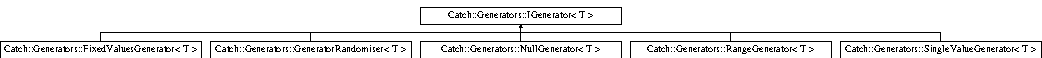
\includegraphics[height=0.783217cm]{struct_catch_1_1_generators_1_1_i_generator}
\end{center}
\end{figure}
\subsection*{Public Member Functions}
\begin{DoxyCompactItemize}
\item 
\mbox{\Hypertarget{struct_catch_1_1_generators_1_1_i_generator_a737a89eb0bff02e580e36c59fb0d1171}\label{struct_catch_1_1_generators_1_1_i_generator_a737a89eb0bff02e580e36c59fb0d1171}} 
virtual auto {\bfseries get} (size\+\_\+t index) const -\/$>$ T=0
\end{DoxyCompactItemize}


The documentation for this struct was generated from the following file\+:\begin{DoxyCompactItemize}
\item 
catch.\+hpp\end{DoxyCompactItemize}

\hypertarget{struct_catch_1_1_i_generator_tracker}{}\section{Catch\+:\+:I\+Generator\+Tracker Struct Reference}
\label{struct_catch_1_1_i_generator_tracker}\index{Catch\+::\+I\+Generator\+Tracker@{Catch\+::\+I\+Generator\+Tracker}}
\subsection*{Public Member Functions}
\begin{DoxyCompactItemize}
\item 
\mbox{\Hypertarget{struct_catch_1_1_i_generator_tracker_ae88084f9af27c8b9a5d5775b9c148498}\label{struct_catch_1_1_i_generator_tracker_ae88084f9af27c8b9a5d5775b9c148498}} 
virtual auto {\bfseries has\+Generator} () const -\/$>$ bool=0
\item 
\mbox{\Hypertarget{struct_catch_1_1_i_generator_tracker_a23be942fc51672598bfa02c678c3078a}\label{struct_catch_1_1_i_generator_tracker_a23be942fc51672598bfa02c678c3078a}} 
virtual auto {\bfseries get\+Generator} () const -\/$>$ Generators\+::\+Generator\+Base\+Ptr const \&=0
\item 
\mbox{\Hypertarget{struct_catch_1_1_i_generator_tracker_a9945eff42219edc5a7071eebd8b0419e}\label{struct_catch_1_1_i_generator_tracker_a9945eff42219edc5a7071eebd8b0419e}} 
virtual void {\bfseries set\+Generator} (Generators\+::\+Generator\+Base\+Ptr \&\&generator)=0
\item 
\mbox{\Hypertarget{struct_catch_1_1_i_generator_tracker_a2922f0d8bc7a732079eadbda78e30f79}\label{struct_catch_1_1_i_generator_tracker_a2922f0d8bc7a732079eadbda78e30f79}} 
virtual auto {\bfseries get\+Index} () const -\/$>$ std\+::size\+\_\+t=0
\end{DoxyCompactItemize}


The documentation for this struct was generated from the following file\+:\begin{DoxyCompactItemize}
\item 
catch.\+hpp\end{DoxyCompactItemize}

\hypertarget{struct_catch_1_1_i_mutable_registry_hub}{}\section{Catch\+:\+:I\+Mutable\+Registry\+Hub Struct Reference}
\label{struct_catch_1_1_i_mutable_registry_hub}\index{Catch\+::\+I\+Mutable\+Registry\+Hub@{Catch\+::\+I\+Mutable\+Registry\+Hub}}
\subsection*{Public Member Functions}
\begin{DoxyCompactItemize}
\item 
\mbox{\Hypertarget{struct_catch_1_1_i_mutable_registry_hub_a1c0ac202ac31ee9f88e8ff5cbac4b243}\label{struct_catch_1_1_i_mutable_registry_hub_a1c0ac202ac31ee9f88e8ff5cbac4b243}} 
virtual void {\bfseries register\+Reporter} (std\+::string const \&name, I\+Reporter\+Factory\+Ptr const \&factory)=0
\item 
\mbox{\Hypertarget{struct_catch_1_1_i_mutable_registry_hub_abd892a133f85581fd00ee75bb379ca56}\label{struct_catch_1_1_i_mutable_registry_hub_abd892a133f85581fd00ee75bb379ca56}} 
virtual void {\bfseries register\+Listener} (I\+Reporter\+Factory\+Ptr const \&factory)=0
\item 
\mbox{\Hypertarget{struct_catch_1_1_i_mutable_registry_hub_a11b85c6744d88c9f83fe16ad4a8dd451}\label{struct_catch_1_1_i_mutable_registry_hub_a11b85c6744d88c9f83fe16ad4a8dd451}} 
virtual void {\bfseries register\+Test} (\mbox{\hyperlink{class_catch_1_1_test_case}{Test\+Case}} const \&test\+Info)=0
\item 
\mbox{\Hypertarget{struct_catch_1_1_i_mutable_registry_hub_ae6825365102693cf7707db022a2c2b49}\label{struct_catch_1_1_i_mutable_registry_hub_ae6825365102693cf7707db022a2c2b49}} 
virtual void {\bfseries register\+Translator} (const \mbox{\hyperlink{struct_catch_1_1_i_exception_translator}{I\+Exception\+Translator}} $\ast$translator)=0
\item 
\mbox{\Hypertarget{struct_catch_1_1_i_mutable_registry_hub_abf2e386b6f94f615719ada711adbf822}\label{struct_catch_1_1_i_mutable_registry_hub_abf2e386b6f94f615719ada711adbf822}} 
virtual void {\bfseries register\+Tag\+Alias} (std\+::string const \&alias, std\+::string const \&tag, \mbox{\hyperlink{struct_catch_1_1_source_line_info}{Source\+Line\+Info}} const \&line\+Info)=0
\item 
\mbox{\Hypertarget{struct_catch_1_1_i_mutable_registry_hub_a72a7d5386851ac3200f8da794a009c86}\label{struct_catch_1_1_i_mutable_registry_hub_a72a7d5386851ac3200f8da794a009c86}} 
virtual void {\bfseries register\+Startup\+Exception} () noexcept=0
\end{DoxyCompactItemize}


The documentation for this struct was generated from the following file\+:\begin{DoxyCompactItemize}
\item 
catch.\+hpp\end{DoxyCompactItemize}

\hypertarget{struct_catch_1_1_i_registry_hub}{}\section{Catch\+:\+:I\+Registry\+Hub Struct Reference}
\label{struct_catch_1_1_i_registry_hub}\index{Catch\+::\+I\+Registry\+Hub@{Catch\+::\+I\+Registry\+Hub}}
\subsection*{Public Member Functions}
\begin{DoxyCompactItemize}
\item 
\mbox{\Hypertarget{struct_catch_1_1_i_registry_hub_a55534563f7ecf7e20ec1e37285ebe54d}\label{struct_catch_1_1_i_registry_hub_a55534563f7ecf7e20ec1e37285ebe54d}} 
virtual I\+Reporter\+Registry const  \& {\bfseries get\+Reporter\+Registry} () const =0
\item 
\mbox{\Hypertarget{struct_catch_1_1_i_registry_hub_af4f6255f0c0f8f1f179fa9d7d4843076}\label{struct_catch_1_1_i_registry_hub_af4f6255f0c0f8f1f179fa9d7d4843076}} 
virtual \mbox{\hyperlink{struct_catch_1_1_i_test_case_registry}{I\+Test\+Case\+Registry}} const  \& {\bfseries get\+Test\+Case\+Registry} () const =0
\item 
\mbox{\Hypertarget{struct_catch_1_1_i_registry_hub_a3c511b1d33e5a6d95c333a0ff387df1a}\label{struct_catch_1_1_i_registry_hub_a3c511b1d33e5a6d95c333a0ff387df1a}} 
virtual I\+Tag\+Alias\+Registry const  \& {\bfseries get\+Tag\+Alias\+Registry} () const =0
\item 
\mbox{\Hypertarget{struct_catch_1_1_i_registry_hub_a48347c170d9c583af73027a27b2f0bd4}\label{struct_catch_1_1_i_registry_hub_a48347c170d9c583af73027a27b2f0bd4}} 
virtual \mbox{\hyperlink{struct_catch_1_1_i_exception_translator_registry}{I\+Exception\+Translator\+Registry}} const  \& {\bfseries get\+Exception\+Translator\+Registry} () const =0
\item 
\mbox{\Hypertarget{struct_catch_1_1_i_registry_hub_a00281210628e6c616aca1d3e0d84db04}\label{struct_catch_1_1_i_registry_hub_a00281210628e6c616aca1d3e0d84db04}} 
virtual Startup\+Exception\+Registry const  \& {\bfseries get\+Startup\+Exception\+Registry} () const =0
\end{DoxyCompactItemize}


The documentation for this struct was generated from the following file\+:\begin{DoxyCompactItemize}
\item 
catch.\+hpp\end{DoxyCompactItemize}

\hypertarget{struct_catch_1_1_i_result_capture}{}\section{Catch\+:\+:I\+Result\+Capture Struct Reference}
\label{struct_catch_1_1_i_result_capture}\index{Catch\+::\+I\+Result\+Capture@{Catch\+::\+I\+Result\+Capture}}
\subsection*{Public Member Functions}
\begin{DoxyCompactItemize}
\item 
\mbox{\Hypertarget{struct_catch_1_1_i_result_capture_a5b76ed52badcb64cf374202e12b81a03}\label{struct_catch_1_1_i_result_capture_a5b76ed52badcb64cf374202e12b81a03}} 
virtual bool {\bfseries section\+Started} (\mbox{\hyperlink{struct_catch_1_1_section_info}{Section\+Info}} const \&section\+Info, \mbox{\hyperlink{struct_catch_1_1_counts}{Counts}} \&assertions)=0
\item 
\mbox{\Hypertarget{struct_catch_1_1_i_result_capture_a4e152bc43dc0933684e31fa67a58195d}\label{struct_catch_1_1_i_result_capture_a4e152bc43dc0933684e31fa67a58195d}} 
virtual void {\bfseries section\+Ended} (\mbox{\hyperlink{struct_catch_1_1_section_end_info}{Section\+End\+Info}} const \&end\+Info)=0
\item 
\mbox{\Hypertarget{struct_catch_1_1_i_result_capture_afcc71eef8ca821ae132cced4a2be6988}\label{struct_catch_1_1_i_result_capture_afcc71eef8ca821ae132cced4a2be6988}} 
virtual void {\bfseries section\+Ended\+Early} (\mbox{\hyperlink{struct_catch_1_1_section_end_info}{Section\+End\+Info}} const \&end\+Info)=0
\item 
\mbox{\Hypertarget{struct_catch_1_1_i_result_capture_ab020d111e29ad1cabe1227dcfda712ef}\label{struct_catch_1_1_i_result_capture_ab020d111e29ad1cabe1227dcfda712ef}} 
virtual auto {\bfseries acquire\+Generator\+Tracker} (\mbox{\hyperlink{struct_catch_1_1_source_line_info}{Source\+Line\+Info}} const \&line\+Info) -\/$>$ \mbox{\hyperlink{struct_catch_1_1_i_generator_tracker}{I\+Generator\+Tracker}} \&=0
\item 
\mbox{\Hypertarget{struct_catch_1_1_i_result_capture_a264ae12330c74b2daae41715a30d51bf}\label{struct_catch_1_1_i_result_capture_a264ae12330c74b2daae41715a30d51bf}} 
virtual void {\bfseries benchmark\+Starting} (Benchmark\+Info const \&info)=0
\item 
\mbox{\Hypertarget{struct_catch_1_1_i_result_capture_a6e5e64f9d94211a888249012ab6cc7fb}\label{struct_catch_1_1_i_result_capture_a6e5e64f9d94211a888249012ab6cc7fb}} 
virtual void {\bfseries benchmark\+Ended} (Benchmark\+Stats const \&stats)=0
\item 
\mbox{\Hypertarget{struct_catch_1_1_i_result_capture_a91d154c1e087e383dcde5aad95cb6a05}\label{struct_catch_1_1_i_result_capture_a91d154c1e087e383dcde5aad95cb6a05}} 
virtual void {\bfseries push\+Scoped\+Message} (\mbox{\hyperlink{struct_catch_1_1_message_info}{Message\+Info}} const \&message)=0
\item 
\mbox{\Hypertarget{struct_catch_1_1_i_result_capture_a42bcb13276706bf8c3ce081ce16d37fd}\label{struct_catch_1_1_i_result_capture_a42bcb13276706bf8c3ce081ce16d37fd}} 
virtual void {\bfseries pop\+Scoped\+Message} (\mbox{\hyperlink{struct_catch_1_1_message_info}{Message\+Info}} const \&message)=0
\item 
\mbox{\Hypertarget{struct_catch_1_1_i_result_capture_a48559e6598ba9474b903697b69c769b2}\label{struct_catch_1_1_i_result_capture_a48559e6598ba9474b903697b69c769b2}} 
virtual void {\bfseries handle\+Fatal\+Error\+Condition} (\mbox{\hyperlink{class_catch_1_1_string_ref}{String\+Ref}} message)=0
\item 
\mbox{\Hypertarget{struct_catch_1_1_i_result_capture_a59a2b05391e464954575d2afb6d5d607}\label{struct_catch_1_1_i_result_capture_a59a2b05391e464954575d2afb6d5d607}} 
virtual void {\bfseries handle\+Expr} (\mbox{\hyperlink{struct_catch_1_1_assertion_info}{Assertion\+Info}} const \&info, \mbox{\hyperlink{struct_catch_1_1_i_transient_expression}{I\+Transient\+Expression}} const \&expr, \mbox{\hyperlink{struct_catch_1_1_assertion_reaction}{Assertion\+Reaction}} \&reaction)=0
\item 
\mbox{\Hypertarget{struct_catch_1_1_i_result_capture_a21788ebc64571abf322b80c8cc51794d}\label{struct_catch_1_1_i_result_capture_a21788ebc64571abf322b80c8cc51794d}} 
virtual void {\bfseries handle\+Message} (\mbox{\hyperlink{struct_catch_1_1_assertion_info}{Assertion\+Info}} const \&info, Result\+Was\+::\+Of\+Type result\+Type, \mbox{\hyperlink{class_catch_1_1_string_ref}{String\+Ref}} const \&message, \mbox{\hyperlink{struct_catch_1_1_assertion_reaction}{Assertion\+Reaction}} \&reaction)=0
\item 
\mbox{\Hypertarget{struct_catch_1_1_i_result_capture_a6382ed20486e2d9a020da971c6d5c53d}\label{struct_catch_1_1_i_result_capture_a6382ed20486e2d9a020da971c6d5c53d}} 
virtual void {\bfseries handle\+Unexpected\+Exception\+Not\+Thrown} (\mbox{\hyperlink{struct_catch_1_1_assertion_info}{Assertion\+Info}} const \&info, \mbox{\hyperlink{struct_catch_1_1_assertion_reaction}{Assertion\+Reaction}} \&reaction)=0
\item 
\mbox{\Hypertarget{struct_catch_1_1_i_result_capture_afc97bc69829185222f955ebeef97adfe}\label{struct_catch_1_1_i_result_capture_afc97bc69829185222f955ebeef97adfe}} 
virtual void {\bfseries handle\+Unexpected\+Inflight\+Exception} (\mbox{\hyperlink{struct_catch_1_1_assertion_info}{Assertion\+Info}} const \&info, std\+::string const \&message, \mbox{\hyperlink{struct_catch_1_1_assertion_reaction}{Assertion\+Reaction}} \&reaction)=0
\item 
\mbox{\Hypertarget{struct_catch_1_1_i_result_capture_a89b89372eb09cc44f8dcad363de6157d}\label{struct_catch_1_1_i_result_capture_a89b89372eb09cc44f8dcad363de6157d}} 
virtual void {\bfseries handle\+Incomplete} (\mbox{\hyperlink{struct_catch_1_1_assertion_info}{Assertion\+Info}} const \&info)=0
\item 
\mbox{\Hypertarget{struct_catch_1_1_i_result_capture_ab7dbdf8aa28427119583e24dbb302c63}\label{struct_catch_1_1_i_result_capture_ab7dbdf8aa28427119583e24dbb302c63}} 
virtual void {\bfseries handle\+Non\+Expr} (\mbox{\hyperlink{struct_catch_1_1_assertion_info}{Assertion\+Info}} const \&info, Result\+Was\+::\+Of\+Type result\+Type, \mbox{\hyperlink{struct_catch_1_1_assertion_reaction}{Assertion\+Reaction}} \&reaction)=0
\item 
\mbox{\Hypertarget{struct_catch_1_1_i_result_capture_a973435fbdcb2f6f07a0ec5719a01e956}\label{struct_catch_1_1_i_result_capture_a973435fbdcb2f6f07a0ec5719a01e956}} 
virtual bool {\bfseries last\+Assertion\+Passed} ()=0
\item 
\mbox{\Hypertarget{struct_catch_1_1_i_result_capture_a9b0ef2cb071e9a9dc6ec1b533026aea7}\label{struct_catch_1_1_i_result_capture_a9b0ef2cb071e9a9dc6ec1b533026aea7}} 
virtual void {\bfseries assertion\+Passed} ()=0
\item 
\mbox{\Hypertarget{struct_catch_1_1_i_result_capture_aea1617f4a84cc648246aa3ed6918b5bf}\label{struct_catch_1_1_i_result_capture_aea1617f4a84cc648246aa3ed6918b5bf}} 
virtual std\+::string {\bfseries get\+Current\+Test\+Name} () const =0
\item 
\mbox{\Hypertarget{struct_catch_1_1_i_result_capture_ab18872c89fab97405a56e9c6a4919736}\label{struct_catch_1_1_i_result_capture_ab18872c89fab97405a56e9c6a4919736}} 
virtual const Assertion\+Result $\ast$ {\bfseries get\+Last\+Result} () const =0
\item 
\mbox{\Hypertarget{struct_catch_1_1_i_result_capture_ae63ecec95db4c236c63ecf616f483810}\label{struct_catch_1_1_i_result_capture_ae63ecec95db4c236c63ecf616f483810}} 
virtual void {\bfseries exception\+Early\+Reported} ()=0
\end{DoxyCompactItemize}


The documentation for this struct was generated from the following file\+:\begin{DoxyCompactItemize}
\item 
catch.\+hpp\end{DoxyCompactItemize}

\hypertarget{struct_catch_1_1_i_runner}{}\section{Catch\+:\+:I\+Runner Struct Reference}
\label{struct_catch_1_1_i_runner}\index{Catch\+::\+I\+Runner@{Catch\+::\+I\+Runner}}
\subsection*{Public Member Functions}
\begin{DoxyCompactItemize}
\item 
\mbox{\Hypertarget{struct_catch_1_1_i_runner_a03713202dd2e041e30b8030088ab0116}\label{struct_catch_1_1_i_runner_a03713202dd2e041e30b8030088ab0116}} 
virtual bool {\bfseries aborting} () const =0
\end{DoxyCompactItemize}


The documentation for this struct was generated from the following file\+:\begin{DoxyCompactItemize}
\item 
catch.\+hpp\end{DoxyCompactItemize}

\hypertarget{struct_catch_1_1is__range}{}\section{Catch\+:\+:is\+\_\+range$<$ T $>$ Struct Template Reference}
\label{struct_catch_1_1is__range}\index{Catch\+::is\+\_\+range$<$ T $>$@{Catch\+::is\+\_\+range$<$ T $>$}}
\subsection*{Static Public Attributes}
\begin{DoxyCompactItemize}
\item 
static const bool {\bfseries value}
\end{DoxyCompactItemize}


\subsection{Member Data Documentation}
\mbox{\Hypertarget{struct_catch_1_1is__range_afaec39e819c3956829cbbd00feba11be}\label{struct_catch_1_1is__range_afaec39e819c3956829cbbd00feba11be}} 
\index{Catch\+::is\+\_\+range@{Catch\+::is\+\_\+range}!value@{value}}
\index{value@{value}!Catch\+::is\+\_\+range@{Catch\+::is\+\_\+range}}
\subsubsection{\texorpdfstring{value}{value}}
{\footnotesize\ttfamily template$<$typename T $>$ \\
const bool \mbox{\hyperlink{struct_catch_1_1is__range}{Catch\+::is\+\_\+range}}$<$ T $>$\+::value\hspace{0.3cm}{\ttfamily [static]}}

{\bfseries Initial value\+:}
\begin{DoxyCode}
=
            !std::is\_same<decltype(begin(std::declval<T>())), not\_this\_one>::value &&
            !std::is\_same<decltype(end(std::declval<T>())), not\_this\_one>::value
\end{DoxyCode}


The documentation for this struct was generated from the following file\+:\begin{DoxyCompactItemize}
\item 
catch.\+hpp\end{DoxyCompactItemize}

\hypertarget{class_catch_1_1_detail_1_1_is_stream_insertable}{}\section{Catch\+:\+:Detail\+:\+:Is\+Stream\+Insertable$<$ T $>$ Class Template Reference}
\label{class_catch_1_1_detail_1_1_is_stream_insertable}\index{Catch\+::\+Detail\+::\+Is\+Stream\+Insertable$<$ T $>$@{Catch\+::\+Detail\+::\+Is\+Stream\+Insertable$<$ T $>$}}
\subsection*{Static Public Attributes}
\begin{DoxyCompactItemize}
\item 
\mbox{\Hypertarget{class_catch_1_1_detail_1_1_is_stream_insertable_a42818b09ae5851126a70ee263769e309}\label{class_catch_1_1_detail_1_1_is_stream_insertable_a42818b09ae5851126a70ee263769e309}} 
static const bool {\bfseries value} = decltype(test$<$std\+::ostream, const T\&$>$(0))\+::value
\end{DoxyCompactItemize}


The documentation for this class was generated from the following file\+:\begin{DoxyCompactItemize}
\item 
catch.\+hpp\end{DoxyCompactItemize}

\hypertarget{struct_catch_1_1_i_stream}{}\section{Catch\+:\+:I\+Stream Struct Reference}
\label{struct_catch_1_1_i_stream}\index{Catch\+::\+I\+Stream@{Catch\+::\+I\+Stream}}
\subsection*{Public Member Functions}
\begin{DoxyCompactItemize}
\item 
\mbox{\Hypertarget{struct_catch_1_1_i_stream_a55a9ddbe250261ff38642f480ebdd902}\label{struct_catch_1_1_i_stream_a55a9ddbe250261ff38642f480ebdd902}} 
virtual std\+::ostream \& {\bfseries stream} () const =0
\end{DoxyCompactItemize}


The documentation for this struct was generated from the following file\+:\begin{DoxyCompactItemize}
\item 
catch.\+hpp\end{DoxyCompactItemize}

\hypertarget{struct_catch_1_1_i_test_case_registry}{}\section{Catch\+:\+:I\+Test\+Case\+Registry Struct Reference}
\label{struct_catch_1_1_i_test_case_registry}\index{Catch\+::\+I\+Test\+Case\+Registry@{Catch\+::\+I\+Test\+Case\+Registry}}
\subsection*{Public Member Functions}
\begin{DoxyCompactItemize}
\item 
\mbox{\Hypertarget{struct_catch_1_1_i_test_case_registry_ad6e4d4a621655123f73ae98cfeda063d}\label{struct_catch_1_1_i_test_case_registry_ad6e4d4a621655123f73ae98cfeda063d}} 
virtual std\+::vector$<$ \mbox{\hyperlink{class_catch_1_1_test_case}{Test\+Case}} $>$ const  \& {\bfseries get\+All\+Tests} () const =0
\item 
\mbox{\Hypertarget{struct_catch_1_1_i_test_case_registry_a33e46639d0319d35497c05bb5d02be5a}\label{struct_catch_1_1_i_test_case_registry_a33e46639d0319d35497c05bb5d02be5a}} 
virtual std\+::vector$<$ \mbox{\hyperlink{class_catch_1_1_test_case}{Test\+Case}} $>$ const  \& {\bfseries get\+All\+Tests\+Sorted} (I\+Config const \&config) const =0
\end{DoxyCompactItemize}


The documentation for this struct was generated from the following file\+:\begin{DoxyCompactItemize}
\item 
catch.\+hpp\end{DoxyCompactItemize}

\hypertarget{struct_catch_1_1_i_test_invoker}{}\section{Catch\+:\+:I\+Test\+Invoker Struct Reference}
\label{struct_catch_1_1_i_test_invoker}\index{Catch\+::\+I\+Test\+Invoker@{Catch\+::\+I\+Test\+Invoker}}
Inheritance diagram for Catch\+:\+:I\+Test\+Invoker\+:\begin{figure}[H]
\begin{center}
\leavevmode
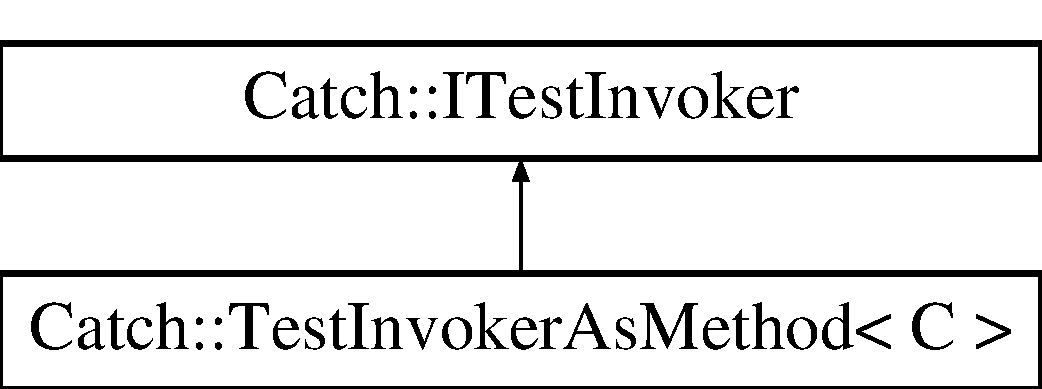
\includegraphics[height=2.000000cm]{struct_catch_1_1_i_test_invoker}
\end{center}
\end{figure}
\subsection*{Public Member Functions}
\begin{DoxyCompactItemize}
\item 
\mbox{\Hypertarget{struct_catch_1_1_i_test_invoker_a6fcd5c5b67d6d5ade6491ff33411ca7f}\label{struct_catch_1_1_i_test_invoker_a6fcd5c5b67d6d5ade6491ff33411ca7f}} 
virtual void {\bfseries invoke} () const =0
\end{DoxyCompactItemize}


The documentation for this struct was generated from the following file\+:\begin{DoxyCompactItemize}
\item 
catch.\+hpp\end{DoxyCompactItemize}

\hypertarget{struct_catch_1_1_i_transient_expression}{}\section{Catch\+:\+:I\+Transient\+Expression Struct Reference}
\label{struct_catch_1_1_i_transient_expression}\index{Catch\+::\+I\+Transient\+Expression@{Catch\+::\+I\+Transient\+Expression}}
Inheritance diagram for Catch\+:\+:I\+Transient\+Expression\+:\begin{figure}[H]
\begin{center}
\leavevmode
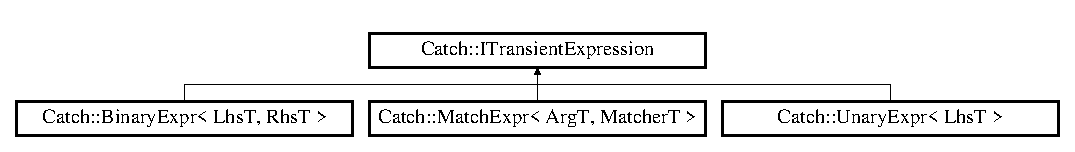
\includegraphics[height=1.588652cm]{struct_catch_1_1_i_transient_expression}
\end{center}
\end{figure}
\subsection*{Public Member Functions}
\begin{DoxyCompactItemize}
\item 
\mbox{\Hypertarget{struct_catch_1_1_i_transient_expression_a3b436e13a0a6d3522bbf70d4e31deb22}\label{struct_catch_1_1_i_transient_expression_a3b436e13a0a6d3522bbf70d4e31deb22}} 
auto {\bfseries is\+Binary\+Expression} () const -\/$>$ bool
\item 
\mbox{\Hypertarget{struct_catch_1_1_i_transient_expression_a101c7db86c87eff93a8ff496720e6320}\label{struct_catch_1_1_i_transient_expression_a101c7db86c87eff93a8ff496720e6320}} 
auto {\bfseries get\+Result} () const -\/$>$ bool
\item 
\mbox{\Hypertarget{struct_catch_1_1_i_transient_expression_aabe1889df9c6e639a24afb08d8a0fe9e}\label{struct_catch_1_1_i_transient_expression_aabe1889df9c6e639a24afb08d8a0fe9e}} 
virtual void {\bfseries stream\+Reconstructed\+Expression} (std\+::ostream \&os) const =0
\item 
\mbox{\Hypertarget{struct_catch_1_1_i_transient_expression_aafe69572b7ed884e63ec81f58d4afd8c}\label{struct_catch_1_1_i_transient_expression_aafe69572b7ed884e63ec81f58d4afd8c}} 
{\bfseries I\+Transient\+Expression} (bool is\+Binary\+Expression, bool result)
\end{DoxyCompactItemize}
\subsection*{Public Attributes}
\begin{DoxyCompactItemize}
\item 
\mbox{\Hypertarget{struct_catch_1_1_i_transient_expression_a75ce48da824d514d08152d396abb28d8}\label{struct_catch_1_1_i_transient_expression_a75ce48da824d514d08152d396abb28d8}} 
bool {\bfseries m\+\_\+is\+Binary\+Expression}
\item 
\mbox{\Hypertarget{struct_catch_1_1_i_transient_expression_a4646e2b5e0156e913653ec3b9b60c942}\label{struct_catch_1_1_i_transient_expression_a4646e2b5e0156e913653ec3b9b60c942}} 
bool {\bfseries m\+\_\+result}
\end{DoxyCompactItemize}


The documentation for this struct was generated from the following file\+:\begin{DoxyCompactItemize}
\item 
catch.\+hpp\end{DoxyCompactItemize}

\hypertarget{class_catch_1_1_lazy_expression}{}\section{Catch\+:\+:Lazy\+Expression Class Reference}
\label{class_catch_1_1_lazy_expression}\index{Catch\+::\+Lazy\+Expression@{Catch\+::\+Lazy\+Expression}}
\subsection*{Public Member Functions}
\begin{DoxyCompactItemize}
\item 
\mbox{\Hypertarget{class_catch_1_1_lazy_expression_a47186c2487bd4bf871e870ba8048553a}\label{class_catch_1_1_lazy_expression_a47186c2487bd4bf871e870ba8048553a}} 
{\bfseries Lazy\+Expression} (bool is\+Negated)
\item 
\mbox{\Hypertarget{class_catch_1_1_lazy_expression_ab82d5e94df0e159b018fbde0170e46f8}\label{class_catch_1_1_lazy_expression_ab82d5e94df0e159b018fbde0170e46f8}} 
{\bfseries Lazy\+Expression} (\mbox{\hyperlink{class_catch_1_1_lazy_expression}{Lazy\+Expression}} const \&other)
\item 
\mbox{\Hypertarget{class_catch_1_1_lazy_expression_ae4ae00d4f36f084c369f2da36565a822}\label{class_catch_1_1_lazy_expression_ae4ae00d4f36f084c369f2da36565a822}} 
\mbox{\hyperlink{class_catch_1_1_lazy_expression}{Lazy\+Expression}} \& {\bfseries operator=} (\mbox{\hyperlink{class_catch_1_1_lazy_expression}{Lazy\+Expression}} const \&)=delete
\item 
\mbox{\Hypertarget{class_catch_1_1_lazy_expression_acdb846cb230cecfc6aca7a925b31fbca}\label{class_catch_1_1_lazy_expression_acdb846cb230cecfc6aca7a925b31fbca}} 
{\bfseries operator bool} () const
\end{DoxyCompactItemize}
\subsection*{Friends}
\begin{DoxyCompactItemize}
\item 
\mbox{\Hypertarget{class_catch_1_1_lazy_expression_a4301a3aa57b612dd8b6ef8461742ecab}\label{class_catch_1_1_lazy_expression_a4301a3aa57b612dd8b6ef8461742ecab}} 
class {\bfseries Assertion\+Handler}
\item 
\mbox{\Hypertarget{class_catch_1_1_lazy_expression_a64019eb137f5ce447cdc71cb80b6e7a4}\label{class_catch_1_1_lazy_expression_a64019eb137f5ce447cdc71cb80b6e7a4}} 
struct {\bfseries Assertion\+Stats}
\item 
\mbox{\Hypertarget{class_catch_1_1_lazy_expression_af3aa096bb29a772bc534830f29a2ce7a}\label{class_catch_1_1_lazy_expression_af3aa096bb29a772bc534830f29a2ce7a}} 
class {\bfseries Run\+Context}
\item 
\mbox{\Hypertarget{class_catch_1_1_lazy_expression_aa01086581cab2fcd2d4580b8fa787dfc}\label{class_catch_1_1_lazy_expression_aa01086581cab2fcd2d4580b8fa787dfc}} 
auto {\bfseries operator$<$$<$} (std\+::ostream \&os, \mbox{\hyperlink{class_catch_1_1_lazy_expression}{Lazy\+Expression}} const \&lazy\+Expr) -\/$>$ std\+::ostream \&
\end{DoxyCompactItemize}


The documentation for this class was generated from the following file\+:\begin{DoxyCompactItemize}
\item 
catch.\+hpp\end{DoxyCompactItemize}

\hypertarget{class_matrix_vector_1_1mat}{}\section{Matrix\+Vector\+:\+:mat Class Reference}
\label{class_matrix_vector_1_1mat}\index{Matrix\+Vector\+::mat@{Matrix\+Vector\+::mat}}
\subsection*{Public Member Functions}
\begin{DoxyCompactItemize}
\item 
\mbox{\Hypertarget{class_matrix_vector_1_1mat_ac6734773d8d3b42b1f2599592fadb8f1}\label{class_matrix_vector_1_1mat_ac6734773d8d3b42b1f2599592fadb8f1}} 
{\bfseries mat} (const \mbox{\hyperlink{class_matrix_vector_1_1mat}{mat}} \&m)
\item 
\mbox{\Hypertarget{class_matrix_vector_1_1mat_ae97f3cb1740056f1aaacde6038c37200}\label{class_matrix_vector_1_1mat_ae97f3cb1740056f1aaacde6038c37200}} 
{\bfseries mat} (int col, int \mbox{\hyperlink{class_matrix_vector_1_1row}{row}})
\item 
\mbox{\Hypertarget{class_matrix_vector_1_1mat_af971b3b347cdb13e134824d386d2b605}\label{class_matrix_vector_1_1mat_af971b3b347cdb13e134824d386d2b605}} 
\mbox{\hyperlink{class_matrix_vector_1_1vec}{vec}} {\bfseries get\+Vec} (int n)
\item 
\mbox{\Hypertarget{class_matrix_vector_1_1mat_acada5c913176b8fa304a4a9d13f8ce3d}\label{class_matrix_vector_1_1mat_acada5c913176b8fa304a4a9d13f8ce3d}} 
\mbox{\hyperlink{class_matrix_vector_1_1row}{row}} {\bfseries get\+Row} (int n)
\item 
\mbox{\Hypertarget{class_matrix_vector_1_1mat_a1539eaf746ccc04ddd9fb44c08c6aecd}\label{class_matrix_vector_1_1mat_a1539eaf746ccc04ddd9fb44c08c6aecd}} 
\mbox{\hyperlink{class_matrix_vector_1_1vec}{vec}} {\bfseries operator$\ast$} (\mbox{\hyperlink{class_matrix_vector_1_1vec}{vec}} \&v)
\item 
\mbox{\Hypertarget{class_matrix_vector_1_1mat_adca8a2d2d0c73d5e35d602b0c0ca858f}\label{class_matrix_vector_1_1mat_adca8a2d2d0c73d5e35d602b0c0ca858f}} 
\mbox{\hyperlink{class_matrix_vector_1_1mat}{mat}} {\bfseries operator$\ast$} (\mbox{\hyperlink{class_matrix_vector_1_1mat}{mat}} \&m)
\item 
\mbox{\Hypertarget{class_matrix_vector_1_1mat_a57c3d94280727f931cefd9ce26c54ec7}\label{class_matrix_vector_1_1mat_a57c3d94280727f931cefd9ce26c54ec7}} 
\mbox{\hyperlink{class_matrix_vector_1_1mat}{mat}} {\bfseries operator=} (const \mbox{\hyperlink{class_matrix_vector_1_1mat}{mat}} \&m)
\item 
\mbox{\Hypertarget{class_matrix_vector_1_1mat_a45be824d6709fea5bcd467d89e41195a}\label{class_matrix_vector_1_1mat_a45be824d6709fea5bcd467d89e41195a}} 
bool {\bfseries operator==} (const \mbox{\hyperlink{class_matrix_vector_1_1mat}{mat}} \&m)
\item 
\mbox{\Hypertarget{class_matrix_vector_1_1mat_a14f1ac703cfed148476a73b4c80327fb}\label{class_matrix_vector_1_1mat_a14f1ac703cfed148476a73b4c80327fb}} 
\mbox{\hyperlink{class_matrix_vector_1_1mat}{mat}} {\bfseries operator+} (\mbox{\hyperlink{class_matrix_vector_1_1mat}{mat}} m)
\item 
\mbox{\Hypertarget{class_matrix_vector_1_1mat_a4f01cc756f0f42ce5015ae1e669f3095}\label{class_matrix_vector_1_1mat_a4f01cc756f0f42ce5015ae1e669f3095}} 
\mbox{\hyperlink{class_matrix_vector_1_1mat}{mat}} {\bfseries operator-\/} (const \mbox{\hyperlink{class_matrix_vector_1_1mat}{mat}} \&m)
\item 
\mbox{\Hypertarget{class_matrix_vector_1_1mat_a79a73fcdbae9745a7b6e537ddc52192e}\label{class_matrix_vector_1_1mat_a79a73fcdbae9745a7b6e537ddc52192e}} 
\mbox{\hyperlink{class_matrix_vector_1_1mat}{mat}} {\bfseries operator/} (float f)
\item 
\mbox{\Hypertarget{class_matrix_vector_1_1mat_a1b1610ba3530c7335c8e6b3320d7550f}\label{class_matrix_vector_1_1mat_a1b1610ba3530c7335c8e6b3320d7550f}} 
\mbox{\hyperlink{class_matrix_vector_1_1mat}{mat}} {\bfseries operator$\ast$} (float f)
\item 
\mbox{\Hypertarget{class_matrix_vector_1_1mat_a69892b8058b8efa67f2b54f6cda8f320}\label{class_matrix_vector_1_1mat_a69892b8058b8efa67f2b54f6cda8f320}} 
\mbox{\hyperlink{class_matrix_vector_1_1mat}{mat}} {\bfseries remove\+Row} (int index)
\item 
\mbox{\Hypertarget{class_matrix_vector_1_1mat_a2b7905669b5952487b36b27c2286a71e}\label{class_matrix_vector_1_1mat_a2b7905669b5952487b36b27c2286a71e}} 
\mbox{\hyperlink{class_matrix_vector_1_1mat}{mat}} {\bfseries remove\+Vec} (int index)
\item 
\mbox{\Hypertarget{class_matrix_vector_1_1mat_a77b5c0d9c96f9819ca7eaf8c95a2a8c0}\label{class_matrix_vector_1_1mat_a77b5c0d9c96f9819ca7eaf8c95a2a8c0}} 
\mbox{\hyperlink{class_matrix_vector_1_1mat}{mat}} {\bfseries insert\+Vec\+Next} (int index, \mbox{\hyperlink{class_matrix_vector_1_1vec}{vec}} v)
\item 
\mbox{\Hypertarget{class_matrix_vector_1_1mat_ab654529acbf45dedea59dc7b0aa4658b}\label{class_matrix_vector_1_1mat_ab654529acbf45dedea59dc7b0aa4658b}} 
\mbox{\hyperlink{class_matrix_vector_1_1mat}{mat}} {\bfseries insert\+Vec\+Previous} (int index, \mbox{\hyperlink{class_matrix_vector_1_1vec}{vec}} v)
\item 
\mbox{\Hypertarget{class_matrix_vector_1_1mat_a08dd3ca70b0dfb818c7512d1ac95b809}\label{class_matrix_vector_1_1mat_a08dd3ca70b0dfb818c7512d1ac95b809}} 
\mbox{\hyperlink{class_matrix_vector_1_1mat}{mat}} {\bfseries clone} ()
\item 
\mbox{\Hypertarget{class_matrix_vector_1_1mat_a07048cbc53f81411fe3be2476aacb4a0}\label{class_matrix_vector_1_1mat_a07048cbc53f81411fe3be2476aacb4a0}} 
\mbox{\hyperlink{class_matrix_vector_1_1mat}{mat}} {\bfseries concat} (\mbox{\hyperlink{class_matrix_vector_1_1mat}{mat}} m)
\item 
\mbox{\Hypertarget{class_matrix_vector_1_1mat_a2e90963266e2c11da30100f8fab7dc54}\label{class_matrix_vector_1_1mat_a2e90963266e2c11da30100f8fab7dc54}} 
\mbox{\hyperlink{class_matrix_vector_1_1mat}{mat}} {\bfseries row\+Multi\+Scala} (int index, float f)
\item 
\mbox{\Hypertarget{class_matrix_vector_1_1mat_af786ab2d8b7bf7b85cf61c9cc76a3cbe}\label{class_matrix_vector_1_1mat_af786ab2d8b7bf7b85cf61c9cc76a3cbe}} 
\mbox{\hyperlink{class_matrix_vector_1_1mat}{mat}} {\bfseries vec\+Multi\+Scala} (int index, float f)
\item 
\mbox{\Hypertarget{class_matrix_vector_1_1mat_a8906d4f0766b3bdac3a45e565ce92616}\label{class_matrix_vector_1_1mat_a8906d4f0766b3bdac3a45e565ce92616}} 
void {\bfseries gene\+Mat} (int init)
\item 
\mbox{\Hypertarget{class_matrix_vector_1_1mat_ae18b1579a3eaef088178cff21f3d6a34}\label{class_matrix_vector_1_1mat_ae18b1579a3eaef088178cff21f3d6a34}} 
void {\bfseries print} ()
\item 
\mbox{\Hypertarget{class_matrix_vector_1_1mat_a5b8a448a9e7e296cb686e75626ffb78a}\label{class_matrix_vector_1_1mat_a5b8a448a9e7e296cb686e75626ffb78a}} 
void {\bfseries zero} ()
\item 
\mbox{\Hypertarget{class_matrix_vector_1_1mat_aed9d65afbbe617320d4dc9af8809fc50}\label{class_matrix_vector_1_1mat_aed9d65afbbe617320d4dc9af8809fc50}} 
void {\bfseries identity} ()
\item 
\mbox{\Hypertarget{class_matrix_vector_1_1mat_ae1062d23d388a0a421ab91b41421a962}\label{class_matrix_vector_1_1mat_ae1062d23d388a0a421ab91b41421a962}} 
\mbox{\hyperlink{class_matrix_vector_1_1mat}{mat}} {\bfseries sub\+Matrix} (int col\+Index, int row\+Index)
\item 
\mbox{\Hypertarget{class_matrix_vector_1_1mat_abe8ff1f6f29fe9e406b755c3f655dd18}\label{class_matrix_vector_1_1mat_abe8ff1f6f29fe9e406b755c3f655dd18}} 
\mbox{\hyperlink{class_matrix_vector_1_1mat}{mat}} {\bfseries transpose} ()
\item 
\mbox{\Hypertarget{class_matrix_vector_1_1mat_aa623e369c2af8582646a44d0c7614db0}\label{class_matrix_vector_1_1mat_aa623e369c2af8582646a44d0c7614db0}} 
\mbox{\hyperlink{class_matrix_vector_1_1mat}{mat}} {\bfseries block} (int col\+Index, int clen, int row\+Index, int rlen)
\item 
\mbox{\Hypertarget{class_matrix_vector_1_1mat_a24f0cefca0d6f79545c2f130fda0b82c}\label{class_matrix_vector_1_1mat_a24f0cefca0d6f79545c2f130fda0b82c}} 
\mbox{\hyperlink{class_matrix_vector_1_1mat}{mat}} {\bfseries take} (int len)
\item 
\mbox{\Hypertarget{class_matrix_vector_1_1mat_a7cd7e57bf6907ee80445afdb462fd095}\label{class_matrix_vector_1_1mat_a7cd7e57bf6907ee80445afdb462fd095}} 
\mbox{\hyperlink{class_matrix_vector_1_1mat}{mat}} {\bfseries drop} (int len)
\item 
\mbox{\Hypertarget{class_matrix_vector_1_1mat_a96ad31de366c370206569f0be9e1de5e}\label{class_matrix_vector_1_1mat_a96ad31de366c370206569f0be9e1de5e}} 
\mbox{\hyperlink{class_matrix_vector_1_1mat}{mat}} {\bfseries init} ()
\item 
\mbox{\Hypertarget{class_matrix_vector_1_1mat_a81893c6dae060972bce5ff67c7a07ee9}\label{class_matrix_vector_1_1mat_a81893c6dae060972bce5ff67c7a07ee9}} 
\mbox{\hyperlink{class_matrix_vector_1_1mat}{mat}} {\bfseries tail} ()
\end{DoxyCompactItemize}
\subsection*{Public Attributes}
\begin{DoxyCompactItemize}
\item 
\mbox{\Hypertarget{class_matrix_vector_1_1mat_a592d970921c2d031bf648d70e5f448dc}\label{class_matrix_vector_1_1mat_a592d970921c2d031bf648d70e5f448dc}} 
int {\bfseries ncol}
\item 
\mbox{\Hypertarget{class_matrix_vector_1_1mat_af448f5d4ef6da3b9c6d72870f690695d}\label{class_matrix_vector_1_1mat_af448f5d4ef6da3b9c6d72870f690695d}} 
int {\bfseries nrow}
\item 
\mbox{\Hypertarget{class_matrix_vector_1_1mat_a5f1dd191eaa81d863fd0c2a546cf7e67}\label{class_matrix_vector_1_1mat_a5f1dd191eaa81d863fd0c2a546cf7e67}} 
float $\ast$$\ast$ {\bfseries arr}
\end{DoxyCompactItemize}


The documentation for this class was generated from the following file\+:\begin{DoxyCompactItemize}
\item 
Aron\+Lib.\+h\end{DoxyCompactItemize}

\hypertarget{struct_catch_1_1_matchers_1_1_impl_1_1_match_all_of}{}\section{Catch\+:\+:Matchers\+:\+:Impl\+:\+:Match\+All\+Of$<$ ArgT $>$ Struct Template Reference}
\label{struct_catch_1_1_matchers_1_1_impl_1_1_match_all_of}\index{Catch\+::\+Matchers\+::\+Impl\+::\+Match\+All\+Of$<$ Arg\+T $>$@{Catch\+::\+Matchers\+::\+Impl\+::\+Match\+All\+Of$<$ Arg\+T $>$}}
Inheritance diagram for Catch\+:\+:Matchers\+:\+:Impl\+:\+:Match\+All\+Of$<$ ArgT $>$\+:\begin{figure}[H]
\begin{center}
\leavevmode
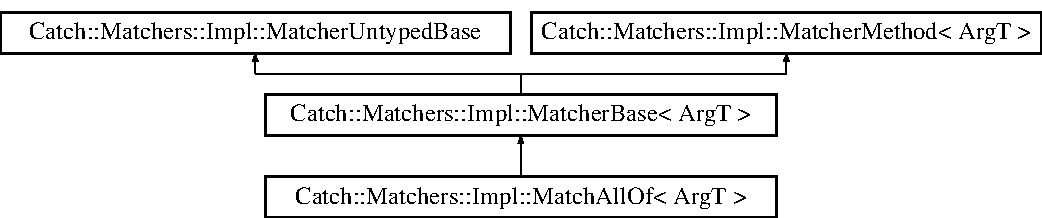
\includegraphics[height=2.926829cm]{struct_catch_1_1_matchers_1_1_impl_1_1_match_all_of}
\end{center}
\end{figure}
\subsection*{Public Member Functions}
\begin{DoxyCompactItemize}
\item 
\mbox{\Hypertarget{struct_catch_1_1_matchers_1_1_impl_1_1_match_all_of_acfb377bda2c58ae62e6df9c3a8a89f8f}\label{struct_catch_1_1_matchers_1_1_impl_1_1_match_all_of_acfb377bda2c58ae62e6df9c3a8a89f8f}} 
bool {\bfseries match} (ArgT const \&arg) const override
\item 
\mbox{\Hypertarget{struct_catch_1_1_matchers_1_1_impl_1_1_match_all_of_acbb9a083e93b546fd33c9235b644c40f}\label{struct_catch_1_1_matchers_1_1_impl_1_1_match_all_of_acbb9a083e93b546fd33c9235b644c40f}} 
std\+::string {\bfseries describe} () const override
\item 
\mbox{\Hypertarget{struct_catch_1_1_matchers_1_1_impl_1_1_match_all_of_a9d0e38b36474336498d627610db434f3}\label{struct_catch_1_1_matchers_1_1_impl_1_1_match_all_of_a9d0e38b36474336498d627610db434f3}} 
\mbox{\hyperlink{struct_catch_1_1_matchers_1_1_impl_1_1_match_all_of}{Match\+All\+Of}}$<$ ArgT $>$ \& {\bfseries operator\&\&} (\mbox{\hyperlink{struct_catch_1_1_matchers_1_1_impl_1_1_matcher_base}{Matcher\+Base}}$<$ ArgT $>$ const \&other)
\end{DoxyCompactItemize}
\subsection*{Public Attributes}
\begin{DoxyCompactItemize}
\item 
\mbox{\Hypertarget{struct_catch_1_1_matchers_1_1_impl_1_1_match_all_of_a98d6a2611f195a4a5c49f92fd877be9a}\label{struct_catch_1_1_matchers_1_1_impl_1_1_match_all_of_a98d6a2611f195a4a5c49f92fd877be9a}} 
std\+::vector$<$ \mbox{\hyperlink{struct_catch_1_1_matchers_1_1_impl_1_1_matcher_base}{Matcher\+Base}}$<$ ArgT $>$ const  $\ast$ $>$ {\bfseries m\+\_\+matchers}
\end{DoxyCompactItemize}
\subsection*{Additional Inherited Members}


The documentation for this struct was generated from the following file\+:\begin{DoxyCompactItemize}
\item 
catch.\+hpp\end{DoxyCompactItemize}

\hypertarget{struct_catch_1_1_matchers_1_1_impl_1_1_match_any_of}{}\section{Catch\+:\+:Matchers\+:\+:Impl\+:\+:Match\+Any\+Of$<$ ArgT $>$ Struct Template Reference}
\label{struct_catch_1_1_matchers_1_1_impl_1_1_match_any_of}\index{Catch\+::\+Matchers\+::\+Impl\+::\+Match\+Any\+Of$<$ Arg\+T $>$@{Catch\+::\+Matchers\+::\+Impl\+::\+Match\+Any\+Of$<$ Arg\+T $>$}}
Inheritance diagram for Catch\+:\+:Matchers\+:\+:Impl\+:\+:Match\+Any\+Of$<$ ArgT $>$\+:\begin{figure}[H]
\begin{center}
\leavevmode
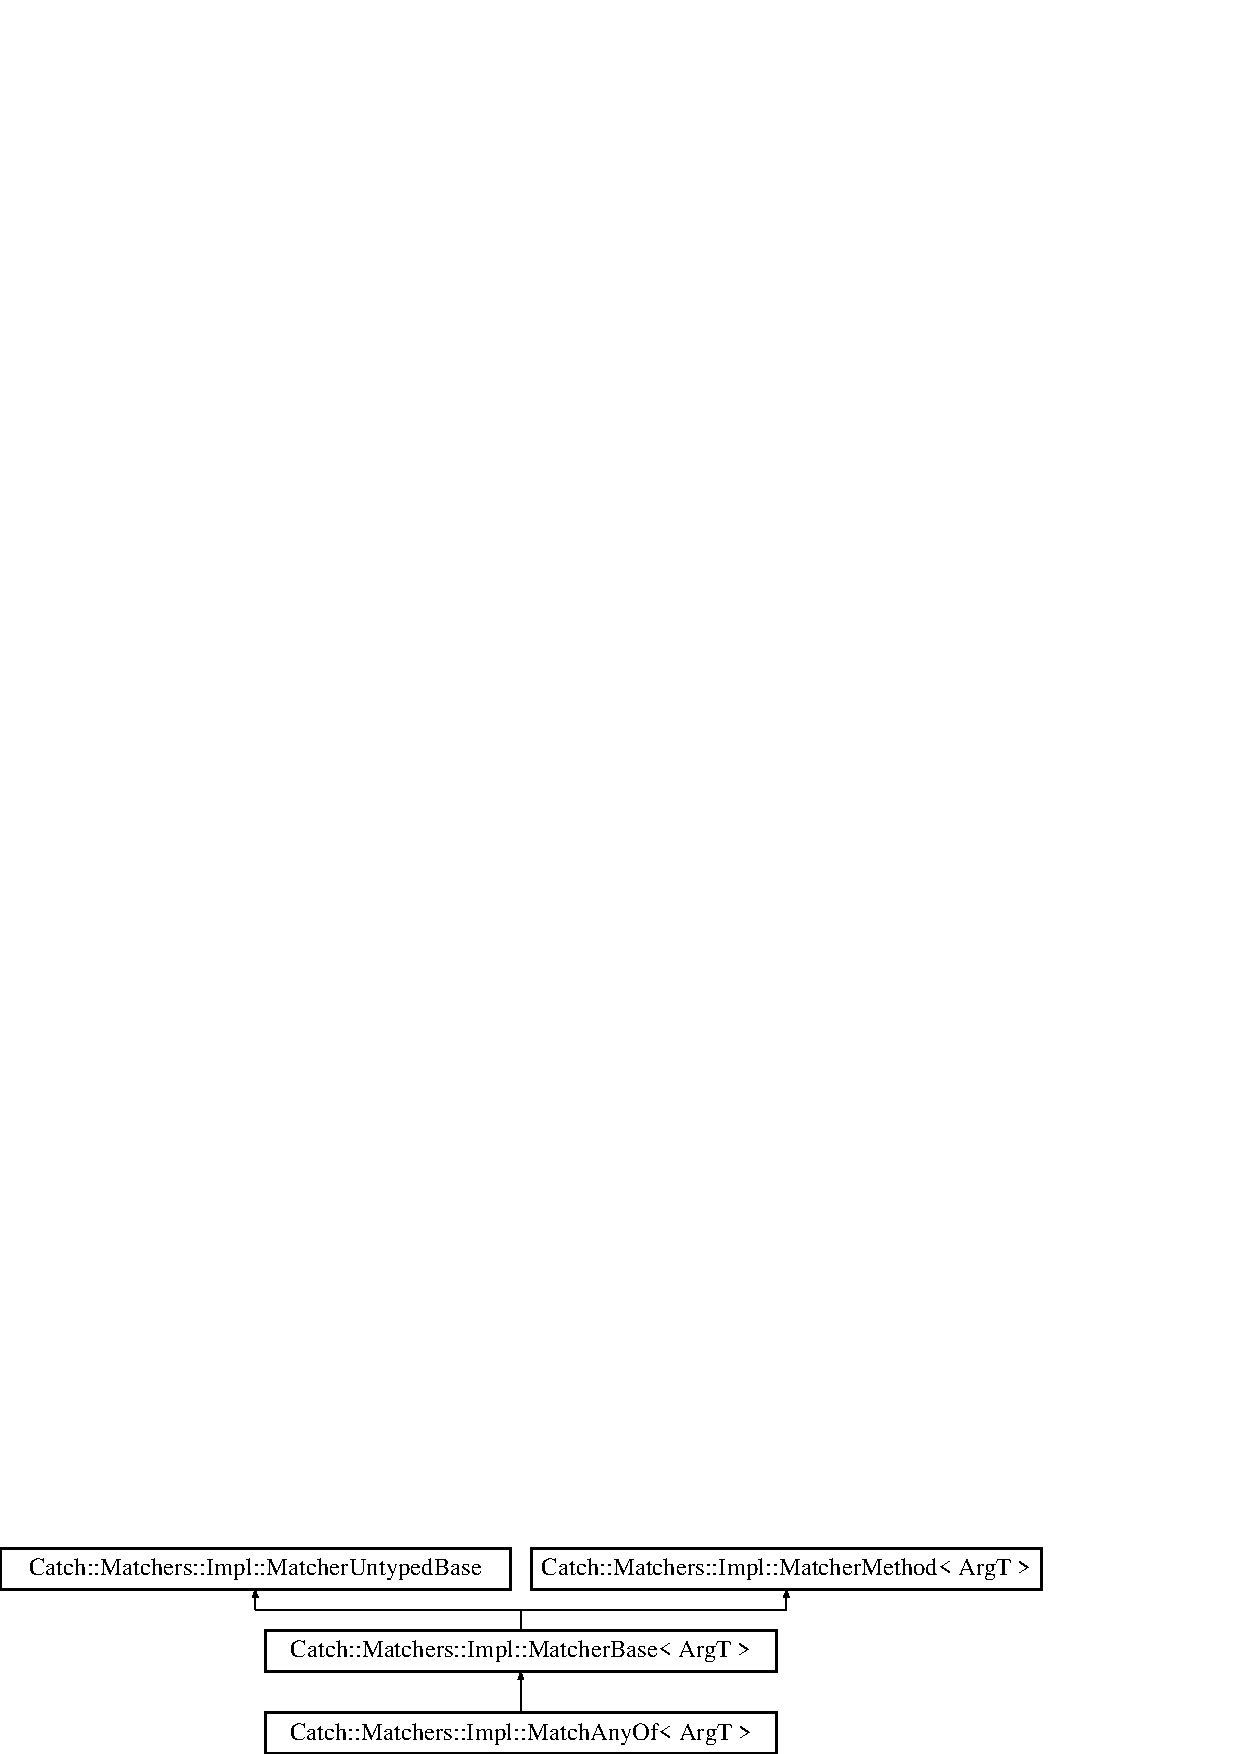
\includegraphics[height=2.926829cm]{struct_catch_1_1_matchers_1_1_impl_1_1_match_any_of}
\end{center}
\end{figure}
\subsection*{Public Member Functions}
\begin{DoxyCompactItemize}
\item 
\mbox{\Hypertarget{struct_catch_1_1_matchers_1_1_impl_1_1_match_any_of_a8a3e8338f979e56277dcf553efb78dc0}\label{struct_catch_1_1_matchers_1_1_impl_1_1_match_any_of_a8a3e8338f979e56277dcf553efb78dc0}} 
bool {\bfseries match} (ArgT const \&arg) const override
\item 
\mbox{\Hypertarget{struct_catch_1_1_matchers_1_1_impl_1_1_match_any_of_a315285204df93d1f8e72f50dd66eb709}\label{struct_catch_1_1_matchers_1_1_impl_1_1_match_any_of_a315285204df93d1f8e72f50dd66eb709}} 
std\+::string {\bfseries describe} () const override
\item 
\mbox{\Hypertarget{struct_catch_1_1_matchers_1_1_impl_1_1_match_any_of_a44d7582dbe09fc31b9a5ba8a6367b506}\label{struct_catch_1_1_matchers_1_1_impl_1_1_match_any_of_a44d7582dbe09fc31b9a5ba8a6367b506}} 
\mbox{\hyperlink{struct_catch_1_1_matchers_1_1_impl_1_1_match_any_of}{Match\+Any\+Of}}$<$ ArgT $>$ \& {\bfseries operator$\vert$$\vert$} (\mbox{\hyperlink{struct_catch_1_1_matchers_1_1_impl_1_1_matcher_base}{Matcher\+Base}}$<$ ArgT $>$ const \&other)
\end{DoxyCompactItemize}
\subsection*{Public Attributes}
\begin{DoxyCompactItemize}
\item 
\mbox{\Hypertarget{struct_catch_1_1_matchers_1_1_impl_1_1_match_any_of_a1fb1119e6110dc15b8d5262ec0aeddd5}\label{struct_catch_1_1_matchers_1_1_impl_1_1_match_any_of_a1fb1119e6110dc15b8d5262ec0aeddd5}} 
std\+::vector$<$ \mbox{\hyperlink{struct_catch_1_1_matchers_1_1_impl_1_1_matcher_base}{Matcher\+Base}}$<$ ArgT $>$ const  $\ast$ $>$ {\bfseries m\+\_\+matchers}
\end{DoxyCompactItemize}
\subsection*{Additional Inherited Members}


The documentation for this struct was generated from the following file\+:\begin{DoxyCompactItemize}
\item 
catch.\+hpp\end{DoxyCompactItemize}

\hypertarget{struct_catch_1_1_matchers_1_1_impl_1_1_matcher_base}{}\section{Catch\+:\+:Matchers\+:\+:Impl\+:\+:Matcher\+Base$<$ T $>$ Struct Template Reference}
\label{struct_catch_1_1_matchers_1_1_impl_1_1_matcher_base}\index{Catch\+::\+Matchers\+::\+Impl\+::\+Matcher\+Base$<$ T $>$@{Catch\+::\+Matchers\+::\+Impl\+::\+Matcher\+Base$<$ T $>$}}
Inheritance diagram for Catch\+:\+:Matchers\+:\+:Impl\+:\+:Matcher\+Base$<$ T $>$\+:\begin{figure}[H]
\begin{center}
\leavevmode
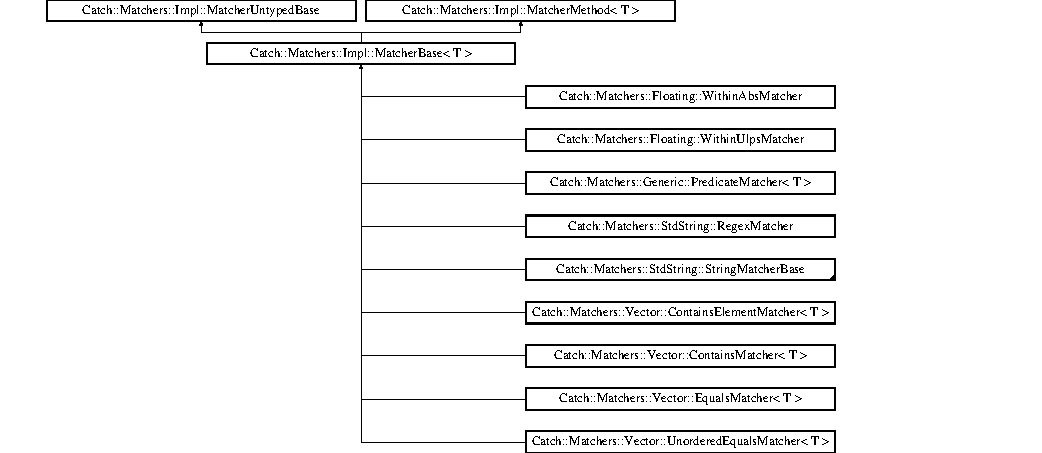
\includegraphics[height=6.092978cm]{struct_catch_1_1_matchers_1_1_impl_1_1_matcher_base}
\end{center}
\end{figure}
\subsection*{Public Member Functions}
\begin{DoxyCompactItemize}
\item 
\mbox{\Hypertarget{struct_catch_1_1_matchers_1_1_impl_1_1_matcher_base_a23c336f6d9457735ddc8dc7ea864d7c9}\label{struct_catch_1_1_matchers_1_1_impl_1_1_matcher_base_a23c336f6d9457735ddc8dc7ea864d7c9}} 
\mbox{\hyperlink{struct_catch_1_1_matchers_1_1_impl_1_1_match_all_of}{Match\+All\+Of}}$<$ T $>$ {\bfseries operator\&\&} (\mbox{\hyperlink{struct_catch_1_1_matchers_1_1_impl_1_1_matcher_base}{Matcher\+Base}} const \&other) const
\item 
\mbox{\Hypertarget{struct_catch_1_1_matchers_1_1_impl_1_1_matcher_base_a5f8542b8f1567a6f9c65d0a6da7b679b}\label{struct_catch_1_1_matchers_1_1_impl_1_1_matcher_base_a5f8542b8f1567a6f9c65d0a6da7b679b}} 
\mbox{\hyperlink{struct_catch_1_1_matchers_1_1_impl_1_1_match_any_of}{Match\+Any\+Of}}$<$ T $>$ {\bfseries operator$\vert$$\vert$} (\mbox{\hyperlink{struct_catch_1_1_matchers_1_1_impl_1_1_matcher_base}{Matcher\+Base}} const \&other) const
\item 
\mbox{\Hypertarget{struct_catch_1_1_matchers_1_1_impl_1_1_matcher_base_a5bb94bf2ff5c7ef73b7c11eb173bdf3b}\label{struct_catch_1_1_matchers_1_1_impl_1_1_matcher_base_a5bb94bf2ff5c7ef73b7c11eb173bdf3b}} 
\mbox{\hyperlink{struct_catch_1_1_matchers_1_1_impl_1_1_match_not_of}{Match\+Not\+Of}}$<$ T $>$ {\bfseries operator!} () const
\end{DoxyCompactItemize}
\subsection*{Additional Inherited Members}


The documentation for this struct was generated from the following file\+:\begin{DoxyCompactItemize}
\item 
catch.\+hpp\end{DoxyCompactItemize}

\hypertarget{struct_catch_1_1_matchers_1_1_impl_1_1_matcher_method}{}\section{Catch\+:\+:Matchers\+:\+:Impl\+:\+:Matcher\+Method$<$ ObjectT $>$ Struct Template Reference}
\label{struct_catch_1_1_matchers_1_1_impl_1_1_matcher_method}\index{Catch\+::\+Matchers\+::\+Impl\+::\+Matcher\+Method$<$ Object\+T $>$@{Catch\+::\+Matchers\+::\+Impl\+::\+Matcher\+Method$<$ Object\+T $>$}}
\subsection*{Public Member Functions}
\begin{DoxyCompactItemize}
\item 
\mbox{\Hypertarget{struct_catch_1_1_matchers_1_1_impl_1_1_matcher_method_ae0920ff9e817acf08e1bb0cbcb044e30}\label{struct_catch_1_1_matchers_1_1_impl_1_1_matcher_method_ae0920ff9e817acf08e1bb0cbcb044e30}} 
virtual bool {\bfseries match} (ObjectT const \&arg) const =0
\end{DoxyCompactItemize}


The documentation for this struct was generated from the following file\+:\begin{DoxyCompactItemize}
\item 
catch.\+hpp\end{DoxyCompactItemize}

\hypertarget{struct_catch_1_1_matchers_1_1_impl_1_1_matcher_method_3_01_ptr_t_01_5_01_4}{}\section{Catch\+:\+:Matchers\+:\+:Impl\+:\+:Matcher\+Method$<$ PtrT $\ast$ $>$ Struct Template Reference}
\label{struct_catch_1_1_matchers_1_1_impl_1_1_matcher_method_3_01_ptr_t_01_5_01_4}\index{Catch\+::\+Matchers\+::\+Impl\+::\+Matcher\+Method$<$ Ptr\+T $\ast$ $>$@{Catch\+::\+Matchers\+::\+Impl\+::\+Matcher\+Method$<$ Ptr\+T $\ast$ $>$}}
\subsection*{Public Member Functions}
\begin{DoxyCompactItemize}
\item 
\mbox{\Hypertarget{struct_catch_1_1_matchers_1_1_impl_1_1_matcher_method_3_01_ptr_t_01_5_01_4_a5fdd64f9509724f32ffc73cb320181d1}\label{struct_catch_1_1_matchers_1_1_impl_1_1_matcher_method_3_01_ptr_t_01_5_01_4_a5fdd64f9509724f32ffc73cb320181d1}} 
virtual bool {\bfseries match} (PtrT $\ast$arg) const =0
\end{DoxyCompactItemize}


The documentation for this struct was generated from the following file\+:\begin{DoxyCompactItemize}
\item 
catch.\+hpp\end{DoxyCompactItemize}

\hypertarget{class_catch_1_1_matchers_1_1_impl_1_1_matcher_untyped_base}{}\section{Catch\+:\+:Matchers\+:\+:Impl\+:\+:Matcher\+Untyped\+Base Class Reference}
\label{class_catch_1_1_matchers_1_1_impl_1_1_matcher_untyped_base}\index{Catch\+::\+Matchers\+::\+Impl\+::\+Matcher\+Untyped\+Base@{Catch\+::\+Matchers\+::\+Impl\+::\+Matcher\+Untyped\+Base}}
Inheritance diagram for Catch\+:\+:Matchers\+:\+:Impl\+:\+:Matcher\+Untyped\+Base\+:\begin{figure}[H]
\begin{center}
\leavevmode
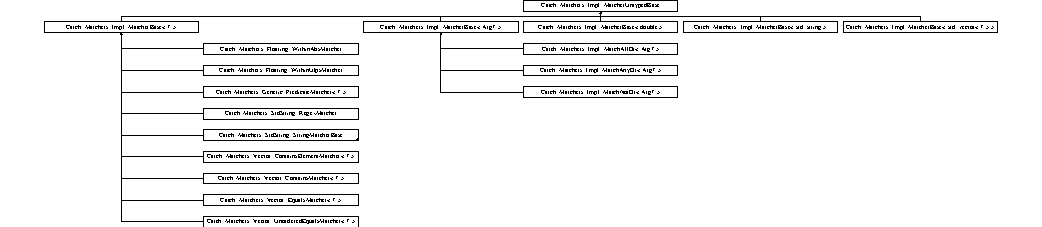
\includegraphics[height=3.046489cm]{class_catch_1_1_matchers_1_1_impl_1_1_matcher_untyped_base}
\end{center}
\end{figure}
\subsection*{Public Member Functions}
\begin{DoxyCompactItemize}
\item 
\mbox{\Hypertarget{class_catch_1_1_matchers_1_1_impl_1_1_matcher_untyped_base_a985fd3c3ffcc9f2e8dc7a330130040b0}\label{class_catch_1_1_matchers_1_1_impl_1_1_matcher_untyped_base_a985fd3c3ffcc9f2e8dc7a330130040b0}} 
{\bfseries Matcher\+Untyped\+Base} (\mbox{\hyperlink{class_catch_1_1_matchers_1_1_impl_1_1_matcher_untyped_base}{Matcher\+Untyped\+Base}} const \&)=default
\item 
\mbox{\Hypertarget{class_catch_1_1_matchers_1_1_impl_1_1_matcher_untyped_base_a62668ccc47b64a9094dcb6413f9af80b}\label{class_catch_1_1_matchers_1_1_impl_1_1_matcher_untyped_base_a62668ccc47b64a9094dcb6413f9af80b}} 
\mbox{\hyperlink{class_catch_1_1_matchers_1_1_impl_1_1_matcher_untyped_base}{Matcher\+Untyped\+Base}} \& {\bfseries operator=} (\mbox{\hyperlink{class_catch_1_1_matchers_1_1_impl_1_1_matcher_untyped_base}{Matcher\+Untyped\+Base}} const \&)=delete
\item 
\mbox{\Hypertarget{class_catch_1_1_matchers_1_1_impl_1_1_matcher_untyped_base_a5982c7c80ca71dfe2298babadad7a453}\label{class_catch_1_1_matchers_1_1_impl_1_1_matcher_untyped_base_a5982c7c80ca71dfe2298babadad7a453}} 
std\+::string {\bfseries to\+String} () const
\end{DoxyCompactItemize}
\subsection*{Protected Member Functions}
\begin{DoxyCompactItemize}
\item 
\mbox{\Hypertarget{class_catch_1_1_matchers_1_1_impl_1_1_matcher_untyped_base_a91d3a907dbfcbb596077df24f6e11fe2}\label{class_catch_1_1_matchers_1_1_impl_1_1_matcher_untyped_base_a91d3a907dbfcbb596077df24f6e11fe2}} 
virtual std\+::string {\bfseries describe} () const =0
\end{DoxyCompactItemize}
\subsection*{Protected Attributes}
\begin{DoxyCompactItemize}
\item 
\mbox{\Hypertarget{class_catch_1_1_matchers_1_1_impl_1_1_matcher_untyped_base_a951095c462657e7097a9a6dc4dde813f}\label{class_catch_1_1_matchers_1_1_impl_1_1_matcher_untyped_base_a951095c462657e7097a9a6dc4dde813f}} 
std\+::string {\bfseries m\+\_\+cached\+To\+String}
\end{DoxyCompactItemize}


The documentation for this class was generated from the following file\+:\begin{DoxyCompactItemize}
\item 
catch.\+hpp\end{DoxyCompactItemize}

\hypertarget{class_catch_1_1_match_expr}{}\section{Catch\+:\+:Match\+Expr$<$ ArgT, MatcherT $>$ Class Template Reference}
\label{class_catch_1_1_match_expr}\index{Catch\+::\+Match\+Expr$<$ Arg\+T, Matcher\+T $>$@{Catch\+::\+Match\+Expr$<$ Arg\+T, Matcher\+T $>$}}
Inheritance diagram for Catch\+:\+:Match\+Expr$<$ ArgT, MatcherT $>$\+:\begin{figure}[H]
\begin{center}
\leavevmode
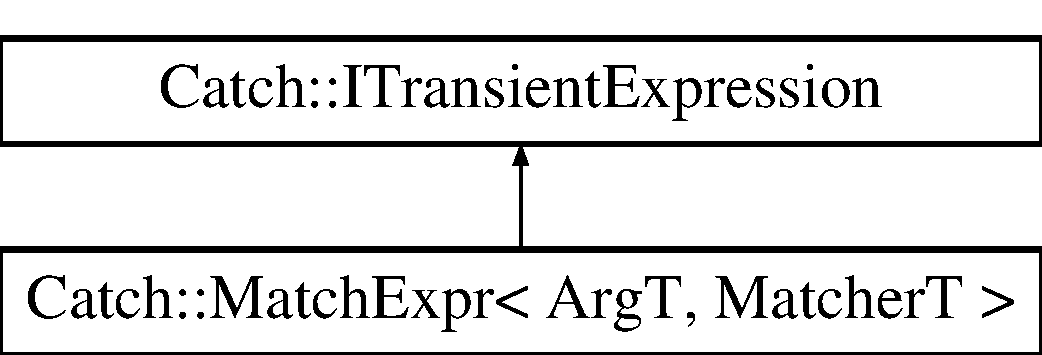
\includegraphics[height=2.000000cm]{class_catch_1_1_match_expr}
\end{center}
\end{figure}
\subsection*{Public Member Functions}
\begin{DoxyCompactItemize}
\item 
\mbox{\Hypertarget{class_catch_1_1_match_expr_ae55ee9bf46c8676c65e9df291a98c345}\label{class_catch_1_1_match_expr_ae55ee9bf46c8676c65e9df291a98c345}} 
{\bfseries Match\+Expr} (ArgT const \&arg, MatcherT const \&matcher, \mbox{\hyperlink{class_catch_1_1_string_ref}{String\+Ref}} const \&matcher\+String)
\item 
\mbox{\Hypertarget{class_catch_1_1_match_expr_ad3e41adb597750b2219bb37e51185629}\label{class_catch_1_1_match_expr_ad3e41adb597750b2219bb37e51185629}} 
void {\bfseries stream\+Reconstructed\+Expression} (std\+::ostream \&os) const override
\end{DoxyCompactItemize}
\subsection*{Additional Inherited Members}


The documentation for this class was generated from the following file\+:\begin{DoxyCompactItemize}
\item 
catch.\+hpp\end{DoxyCompactItemize}

\hypertarget{struct_catch_1_1_matchers_1_1_impl_1_1_match_not_of}{}\section{Catch\+:\+:Matchers\+:\+:Impl\+:\+:Match\+Not\+Of$<$ ArgT $>$ Struct Template Reference}
\label{struct_catch_1_1_matchers_1_1_impl_1_1_match_not_of}\index{Catch\+::\+Matchers\+::\+Impl\+::\+Match\+Not\+Of$<$ Arg\+T $>$@{Catch\+::\+Matchers\+::\+Impl\+::\+Match\+Not\+Of$<$ Arg\+T $>$}}
Inheritance diagram for Catch\+:\+:Matchers\+:\+:Impl\+:\+:Match\+Not\+Of$<$ ArgT $>$\+:\begin{figure}[H]
\begin{center}
\leavevmode
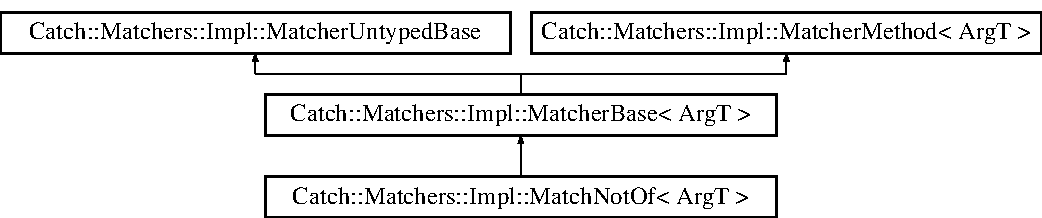
\includegraphics[height=2.926829cm]{struct_catch_1_1_matchers_1_1_impl_1_1_match_not_of}
\end{center}
\end{figure}
\subsection*{Public Member Functions}
\begin{DoxyCompactItemize}
\item 
\mbox{\Hypertarget{struct_catch_1_1_matchers_1_1_impl_1_1_match_not_of_a47afdd9e4c3354cef85adc3186097ae4}\label{struct_catch_1_1_matchers_1_1_impl_1_1_match_not_of_a47afdd9e4c3354cef85adc3186097ae4}} 
{\bfseries Match\+Not\+Of} (\mbox{\hyperlink{struct_catch_1_1_matchers_1_1_impl_1_1_matcher_base}{Matcher\+Base}}$<$ ArgT $>$ const \&underlying\+Matcher)
\item 
\mbox{\Hypertarget{struct_catch_1_1_matchers_1_1_impl_1_1_match_not_of_a181d693c0258e582d80dc6117a1f2b66}\label{struct_catch_1_1_matchers_1_1_impl_1_1_match_not_of_a181d693c0258e582d80dc6117a1f2b66}} 
bool {\bfseries match} (ArgT const \&arg) const override
\item 
\mbox{\Hypertarget{struct_catch_1_1_matchers_1_1_impl_1_1_match_not_of_ac5fb4ef6a9069d23a4098c3c818f06b0}\label{struct_catch_1_1_matchers_1_1_impl_1_1_match_not_of_ac5fb4ef6a9069d23a4098c3c818f06b0}} 
std\+::string {\bfseries describe} () const override
\end{DoxyCompactItemize}
\subsection*{Public Attributes}
\begin{DoxyCompactItemize}
\item 
\mbox{\Hypertarget{struct_catch_1_1_matchers_1_1_impl_1_1_match_not_of_af7ac67f112b0e93796b048a47329aad4}\label{struct_catch_1_1_matchers_1_1_impl_1_1_match_not_of_af7ac67f112b0e93796b048a47329aad4}} 
\mbox{\hyperlink{struct_catch_1_1_matchers_1_1_impl_1_1_matcher_base}{Matcher\+Base}}$<$ ArgT $>$ const  \& {\bfseries m\+\_\+underlying\+Matcher}
\end{DoxyCompactItemize}
\subsection*{Additional Inherited Members}


The documentation for this struct was generated from the following file\+:\begin{DoxyCompactItemize}
\item 
catch.\+hpp\end{DoxyCompactItemize}

\hypertarget{class_space_matrix4_1_1_matrix4}{}\section{Space\+Matrix4\+:\+:Matrix4 Class Reference}
\label{class_space_matrix4_1_1_matrix4}\index{Space\+Matrix4\+::\+Matrix4@{Space\+Matrix4\+::\+Matrix4}}
\subsection*{Public Member Functions}
\begin{DoxyCompactItemize}
\item 
\mbox{\Hypertarget{class_space_matrix4_1_1_matrix4_ae3b3ede099369c664e4ed51ec181437d}\label{class_space_matrix4_1_1_matrix4_ae3b3ede099369c664e4ed51ec181437d}} 
{\bfseries Matrix4} (const \mbox{\hyperlink{class_space_matrix4_1_1_matrix4}{Matrix4}} \&matrix)
\item 
\mbox{\Hypertarget{class_space_matrix4_1_1_matrix4_ad02fd76e843b890744b950e73fc0c4a2}\label{class_space_matrix4_1_1_matrix4_ad02fd76e843b890744b950e73fc0c4a2}} 
{\bfseries Matrix4} (\mbox{\hyperlink{class_space_vector4_1_1_vector4}{Vector4}} v0, \mbox{\hyperlink{class_space_vector4_1_1_vector4}{Vector4}} v1, \mbox{\hyperlink{class_space_vector4_1_1_vector4}{Vector4}} v2, \mbox{\hyperlink{class_space_vector4_1_1_vector4}{Vector4}} v3)
\item 
\mbox{\Hypertarget{class_space_matrix4_1_1_matrix4_a4e95830c4932dbeba8ba5634bdb43740}\label{class_space_matrix4_1_1_matrix4_a4e95830c4932dbeba8ba5634bdb43740}} 
{\bfseries Matrix4} (float m\mbox{[}16\mbox{]})
\item 
\mbox{\Hypertarget{class_space_matrix4_1_1_matrix4_acb7db0fb04a6088c08e14f2fe303f1c7}\label{class_space_matrix4_1_1_matrix4_acb7db0fb04a6088c08e14f2fe303f1c7}} 
\mbox{\hyperlink{class_space_matrix4_1_1_matrix4}{Matrix4}} \& {\bfseries operator=} (const \mbox{\hyperlink{class_space_matrix4_1_1_matrix4}{Matrix4}} \&matrix)
\item 
\mbox{\Hypertarget{class_space_matrix4_1_1_matrix4_ae53e7683f380bb20dd16150bc065eac2}\label{class_space_matrix4_1_1_matrix4_ae53e7683f380bb20dd16150bc065eac2}} 
bool {\bfseries operator==} (const \mbox{\hyperlink{class_space_matrix4_1_1_matrix4}{Matrix4}} \&matrix)
\item 
\mbox{\Hypertarget{class_space_matrix4_1_1_matrix4_aa24d8b4b5168739faedb27ea94608f47}\label{class_space_matrix4_1_1_matrix4_aa24d8b4b5168739faedb27ea94608f47}} 
const \mbox{\hyperlink{class_space_vector4_1_1_vector4}{Vector4}} \& {\bfseries operator\mbox{[}$\,$\mbox{]}} (int index) const
\item 
\mbox{\Hypertarget{class_space_matrix4_1_1_matrix4_a5177148ed3ae31f6c5642566c5db15c9}\label{class_space_matrix4_1_1_matrix4_a5177148ed3ae31f6c5642566c5db15c9}} 
\mbox{\hyperlink{class_space_vector4_1_1_vector4}{Vector4}} \& {\bfseries operator\mbox{[}$\,$\mbox{]}} (int index)
\item 
\mbox{\Hypertarget{class_space_matrix4_1_1_matrix4_a8d1107457f530451bc6c871c29c09ecd}\label{class_space_matrix4_1_1_matrix4_a8d1107457f530451bc6c871c29c09ecd}} 
\mbox{\hyperlink{class_space_matrix4_1_1_matrix4}{Matrix4}} {\bfseries operator+} (\mbox{\hyperlink{class_space_matrix4_1_1_matrix4}{Matrix4}} \&rhs)
\item 
\mbox{\Hypertarget{class_space_matrix4_1_1_matrix4_aaf4abf8264697a38c7ece5a916f924f2}\label{class_space_matrix4_1_1_matrix4_aaf4abf8264697a38c7ece5a916f924f2}} 
\mbox{\hyperlink{class_space_matrix4_1_1_matrix4}{Matrix4}} {\bfseries operator-\/} (\mbox{\hyperlink{class_space_matrix4_1_1_matrix4}{Matrix4}} \&rhs)
\item 
\mbox{\Hypertarget{class_space_matrix4_1_1_matrix4_a6818fd388797ac3b8df61dccc2efd255}\label{class_space_matrix4_1_1_matrix4_a6818fd388797ac3b8df61dccc2efd255}} 
\mbox{\hyperlink{class_space_vector4_1_1_vector4}{Vector4}} {\bfseries operator$\ast$} (\mbox{\hyperlink{class_space_vector4_1_1_vector4}{Vector4}} \&vect4)
\item 
\mbox{\Hypertarget{class_space_matrix4_1_1_matrix4_a6de63705c52bff6ade591a85ddf7cde0}\label{class_space_matrix4_1_1_matrix4_a6de63705c52bff6ade591a85ddf7cde0}} 
\mbox{\hyperlink{class_space_matrix4_1_1_matrix4}{Matrix4}} {\bfseries operator$\ast$} (\mbox{\hyperlink{class_space_matrix4_1_1_matrix4}{Matrix4}} \&matrix)
\item 
\mbox{\Hypertarget{class_space_matrix4_1_1_matrix4_ad0f454fdc02a1f37aa658494f61a931d}\label{class_space_matrix4_1_1_matrix4_ad0f454fdc02a1f37aa658494f61a931d}} 
\mbox{\hyperlink{class_space_matrix4_1_1_matrix4}{Matrix4}} {\bfseries translate} (float x, float y, float z)
\item 
\mbox{\Hypertarget{class_space_matrix4_1_1_matrix4_abb89178eaa1deef275886df0d19b50e6}\label{class_space_matrix4_1_1_matrix4_abb89178eaa1deef275886df0d19b50e6}} 
\mbox{\hyperlink{class_space_matrix4_1_1_matrix4}{Matrix4}} {\bfseries identity} ()
\item 
\mbox{\Hypertarget{class_space_matrix4_1_1_matrix4_a225dbeed5391fdc5de3c4799308f838c}\label{class_space_matrix4_1_1_matrix4_a225dbeed5391fdc5de3c4799308f838c}} 
void {\bfseries pp} ()
\item 
\mbox{\Hypertarget{class_space_matrix4_1_1_matrix4_a6c8365b645a26a77a5fca5411b25097e}\label{class_space_matrix4_1_1_matrix4_a6c8365b645a26a77a5fca5411b25097e}} 
void {\bfseries print} ()
\end{DoxyCompactItemize}


The documentation for this class was generated from the following file\+:\begin{DoxyCompactItemize}
\item 
Aron\+Lib.\+h\end{DoxyCompactItemize}

\hypertarget{struct_catch_1_1_message_builder}{}\section{Catch\+:\+:Message\+Builder Struct Reference}
\label{struct_catch_1_1_message_builder}\index{Catch\+::\+Message\+Builder@{Catch\+::\+Message\+Builder}}
Inheritance diagram for Catch\+:\+:Message\+Builder\+:\begin{figure}[H]
\begin{center}
\leavevmode
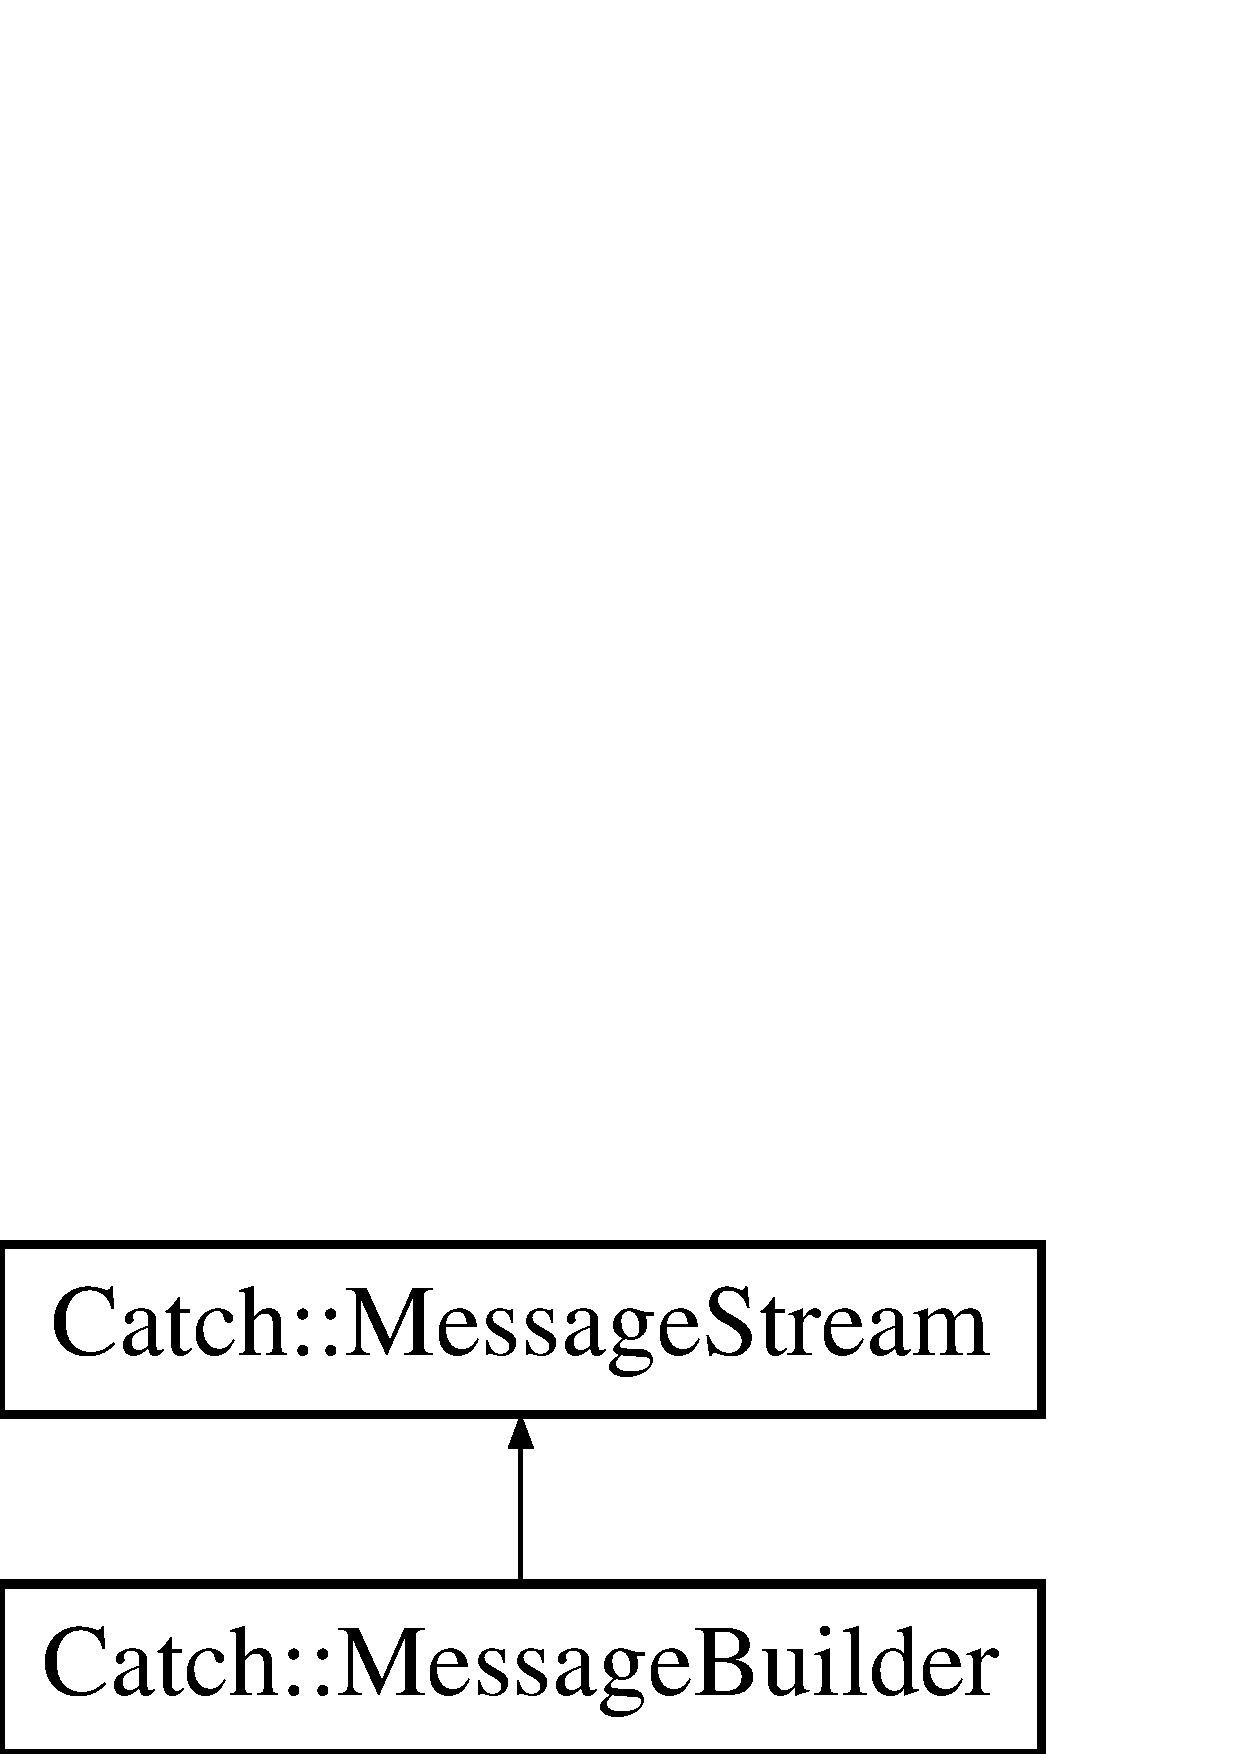
\includegraphics[height=2.000000cm]{struct_catch_1_1_message_builder}
\end{center}
\end{figure}
\subsection*{Public Member Functions}
\begin{DoxyCompactItemize}
\item 
\mbox{\Hypertarget{struct_catch_1_1_message_builder_ac34832ca527a758f000ac233d32dd068}\label{struct_catch_1_1_message_builder_ac34832ca527a758f000ac233d32dd068}} 
{\bfseries Message\+Builder} (\mbox{\hyperlink{class_catch_1_1_string_ref}{String\+Ref}} const \&macro\+Name, \mbox{\hyperlink{struct_catch_1_1_source_line_info}{Source\+Line\+Info}} const \&line\+Info, Result\+Was\+::\+Of\+Type type)
\item 
\mbox{\Hypertarget{struct_catch_1_1_message_builder_a20fa48d069b20dddcc2d3df8abb123c1}\label{struct_catch_1_1_message_builder_a20fa48d069b20dddcc2d3df8abb123c1}} 
{\footnotesize template$<$typename T $>$ }\\\mbox{\hyperlink{struct_catch_1_1_message_builder}{Message\+Builder}} \& {\bfseries operator$<$$<$} (T const \&value)
\end{DoxyCompactItemize}
\subsection*{Public Attributes}
\begin{DoxyCompactItemize}
\item 
\mbox{\Hypertarget{struct_catch_1_1_message_builder_a979f1c2b36d78f80ee275bfa5ba0209f}\label{struct_catch_1_1_message_builder_a979f1c2b36d78f80ee275bfa5ba0209f}} 
\mbox{\hyperlink{struct_catch_1_1_message_info}{Message\+Info}} {\bfseries m\+\_\+info}
\end{DoxyCompactItemize}


The documentation for this struct was generated from the following file\+:\begin{DoxyCompactItemize}
\item 
catch.\+hpp\end{DoxyCompactItemize}

\hypertarget{struct_catch_1_1_message_info}{}\section{Catch\+:\+:Message\+Info Struct Reference}
\label{struct_catch_1_1_message_info}\index{Catch\+::\+Message\+Info@{Catch\+::\+Message\+Info}}
\subsection*{Public Member Functions}
\begin{DoxyCompactItemize}
\item 
\mbox{\Hypertarget{struct_catch_1_1_message_info_afac7a84a9e8655428035a3c5418044f0}\label{struct_catch_1_1_message_info_afac7a84a9e8655428035a3c5418044f0}} 
{\bfseries Message\+Info} (\mbox{\hyperlink{class_catch_1_1_string_ref}{String\+Ref}} const \&\+\_\+macro\+Name, \mbox{\hyperlink{struct_catch_1_1_source_line_info}{Source\+Line\+Info}} const \&\+\_\+line\+Info, Result\+Was\+::\+Of\+Type \+\_\+type)
\item 
\mbox{\Hypertarget{struct_catch_1_1_message_info_af4b37f2172ba55395813b4bb6bbbde1a}\label{struct_catch_1_1_message_info_af4b37f2172ba55395813b4bb6bbbde1a}} 
bool {\bfseries operator==} (\mbox{\hyperlink{struct_catch_1_1_message_info}{Message\+Info}} const \&other) const
\item 
\mbox{\Hypertarget{struct_catch_1_1_message_info_a8254cb8fca2da02a29a9843cdcb79df1}\label{struct_catch_1_1_message_info_a8254cb8fca2da02a29a9843cdcb79df1}} 
bool {\bfseries operator$<$} (\mbox{\hyperlink{struct_catch_1_1_message_info}{Message\+Info}} const \&other) const
\end{DoxyCompactItemize}
\subsection*{Public Attributes}
\begin{DoxyCompactItemize}
\item 
\mbox{\Hypertarget{struct_catch_1_1_message_info_a3ee7cd41def0989d2193bad7101436a0}\label{struct_catch_1_1_message_info_a3ee7cd41def0989d2193bad7101436a0}} 
\mbox{\hyperlink{class_catch_1_1_string_ref}{String\+Ref}} {\bfseries macro\+Name}
\item 
\mbox{\Hypertarget{struct_catch_1_1_message_info_ab6cd06e050bf426c6577502a5c50e256}\label{struct_catch_1_1_message_info_ab6cd06e050bf426c6577502a5c50e256}} 
std\+::string {\bfseries message}
\item 
\mbox{\Hypertarget{struct_catch_1_1_message_info_a985165328723e599696ebd8e43195cc5}\label{struct_catch_1_1_message_info_a985165328723e599696ebd8e43195cc5}} 
\mbox{\hyperlink{struct_catch_1_1_source_line_info}{Source\+Line\+Info}} {\bfseries line\+Info}
\item 
\mbox{\Hypertarget{struct_catch_1_1_message_info_ae928b9117465c696e45951d9d0284e78}\label{struct_catch_1_1_message_info_ae928b9117465c696e45951d9d0284e78}} 
Result\+Was\+::\+Of\+Type {\bfseries type}
\item 
\mbox{\Hypertarget{struct_catch_1_1_message_info_a7f4f57ea21e50160adefce7b68a781d6}\label{struct_catch_1_1_message_info_a7f4f57ea21e50160adefce7b68a781d6}} 
unsigned int {\bfseries sequence}
\end{DoxyCompactItemize}


The documentation for this struct was generated from the following file\+:\begin{DoxyCompactItemize}
\item 
catch.\+hpp\end{DoxyCompactItemize}

\hypertarget{struct_catch_1_1_message_stream}{}\section{Catch\+:\+:Message\+Stream Struct Reference}
\label{struct_catch_1_1_message_stream}\index{Catch\+::\+Message\+Stream@{Catch\+::\+Message\+Stream}}
Inheritance diagram for Catch\+:\+:Message\+Stream\+:\begin{figure}[H]
\begin{center}
\leavevmode
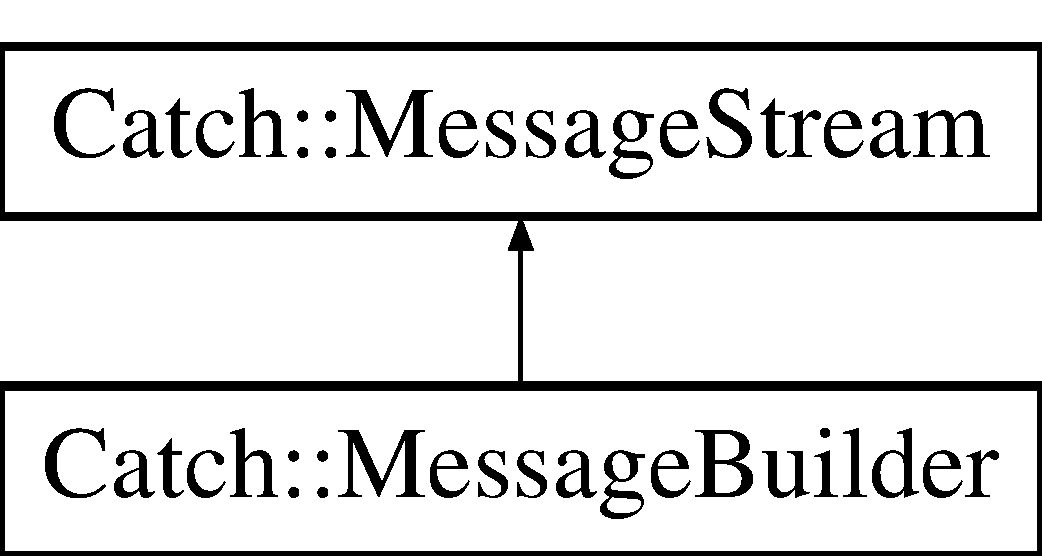
\includegraphics[height=2.000000cm]{struct_catch_1_1_message_stream}
\end{center}
\end{figure}
\subsection*{Public Member Functions}
\begin{DoxyCompactItemize}
\item 
\mbox{\Hypertarget{struct_catch_1_1_message_stream_a554c4aff5925a077e9fe9d858217428d}\label{struct_catch_1_1_message_stream_a554c4aff5925a077e9fe9d858217428d}} 
{\footnotesize template$<$typename T $>$ }\\\mbox{\hyperlink{struct_catch_1_1_message_stream}{Message\+Stream}} \& {\bfseries operator$<$$<$} (T const \&value)
\end{DoxyCompactItemize}
\subsection*{Public Attributes}
\begin{DoxyCompactItemize}
\item 
\mbox{\Hypertarget{struct_catch_1_1_message_stream_a9202520faed8882ef469db9f353ec578}\label{struct_catch_1_1_message_stream_a9202520faed8882ef469db9f353ec578}} 
\mbox{\hyperlink{class_catch_1_1_reusable_string_stream}{Reusable\+String\+Stream}} {\bfseries m\+\_\+stream}
\end{DoxyCompactItemize}


The documentation for this struct was generated from the following file\+:\begin{DoxyCompactItemize}
\item 
catch.\+hpp\end{DoxyCompactItemize}

\hypertarget{struct_catch_1_1_name_and_tags}{}\section{Catch\+:\+:Name\+And\+Tags Struct Reference}
\label{struct_catch_1_1_name_and_tags}\index{Catch\+::\+Name\+And\+Tags@{Catch\+::\+Name\+And\+Tags}}
\subsection*{Public Member Functions}
\begin{DoxyCompactItemize}
\item 
\mbox{\Hypertarget{struct_catch_1_1_name_and_tags_ab585111e615ce8c504a2b9630de8ee94}\label{struct_catch_1_1_name_and_tags_ab585111e615ce8c504a2b9630de8ee94}} 
{\bfseries Name\+And\+Tags} (\mbox{\hyperlink{class_catch_1_1_string_ref}{String\+Ref}} const \&name\+\_\+=\mbox{\hyperlink{class_catch_1_1_string_ref}{String\+Ref}}(), \mbox{\hyperlink{class_catch_1_1_string_ref}{String\+Ref}} const \&tags\+\_\+=\mbox{\hyperlink{class_catch_1_1_string_ref}{String\+Ref}}()) noexcept
\end{DoxyCompactItemize}
\subsection*{Public Attributes}
\begin{DoxyCompactItemize}
\item 
\mbox{\Hypertarget{struct_catch_1_1_name_and_tags_a7cbea60e0cebfa622c667008eb011420}\label{struct_catch_1_1_name_and_tags_a7cbea60e0cebfa622c667008eb011420}} 
\mbox{\hyperlink{class_catch_1_1_string_ref}{String\+Ref}} {\bfseries name}
\item 
\mbox{\Hypertarget{struct_catch_1_1_name_and_tags_a74062ed1138834a348424eb7ed900c57}\label{struct_catch_1_1_name_and_tags_a74062ed1138834a348424eb7ed900c57}} 
\mbox{\hyperlink{class_catch_1_1_string_ref}{String\+Ref}} {\bfseries tags}
\end{DoxyCompactItemize}


The documentation for this struct was generated from the following file\+:\begin{DoxyCompactItemize}
\item 
catch.\+hpp\end{DoxyCompactItemize}

\hypertarget{class_node}{}\section{Node$<$ Type $>$ Class Template Reference}
\label{class_node}\index{Node$<$ Type $>$@{Node$<$ Type $>$}}
\subsection*{Public Member Functions}
\begin{DoxyCompactItemize}
\item 
\mbox{\Hypertarget{class_node_ab71076020d4a5e98653d54ac81610cd8}\label{class_node_ab71076020d4a5e98653d54ac81610cd8}} 
{\bfseries Node} (Type n)
\end{DoxyCompactItemize}
\subsection*{Public Attributes}
\begin{DoxyCompactItemize}
\item 
\mbox{\Hypertarget{class_node_a0659c1cb99599bedd163d63603fe0bb7}\label{class_node_a0659c1cb99599bedd163d63603fe0bb7}} 
\mbox{\hyperlink{class_node}{Node}} $\ast$ {\bfseries next}
\item 
\mbox{\Hypertarget{class_node_abb08a8b3137dd8fc8874348a439e01b4}\label{class_node_abb08a8b3137dd8fc8874348a439e01b4}} 
\mbox{\hyperlink{class_node}{Node}} $\ast$ {\bfseries left}
\item 
\mbox{\Hypertarget{class_node_a34452c0684d3cb1590406ad201b43e65}\label{class_node_a34452c0684d3cb1590406ad201b43e65}} 
\mbox{\hyperlink{class_node}{Node}} $\ast$ {\bfseries right}
\item 
\mbox{\Hypertarget{class_node_af46472827dd148b7e22fc863d2a95aa5}\label{class_node_af46472827dd148b7e22fc863d2a95aa5}} 
\mbox{\hyperlink{class_node}{Node}} $\ast$ {\bfseries prev}
\item 
\mbox{\Hypertarget{class_node_a9c844a942f0c368060d663bfa7418cbe}\label{class_node_a9c844a942f0c368060d663bfa7418cbe}} 
Type {\bfseries data}
\end{DoxyCompactItemize}


The documentation for this class was generated from the following file\+:\begin{DoxyCompactItemize}
\item 
Node.\+h\end{DoxyCompactItemize}

\hypertarget{class_catch_1_1_non_copyable}{}\section{Catch\+:\+:Non\+Copyable Class Reference}
\label{class_catch_1_1_non_copyable}\index{Catch\+::\+Non\+Copyable@{Catch\+::\+Non\+Copyable}}
Inheritance diagram for Catch\+:\+:Non\+Copyable\+:\begin{figure}[H]
\begin{center}
\leavevmode
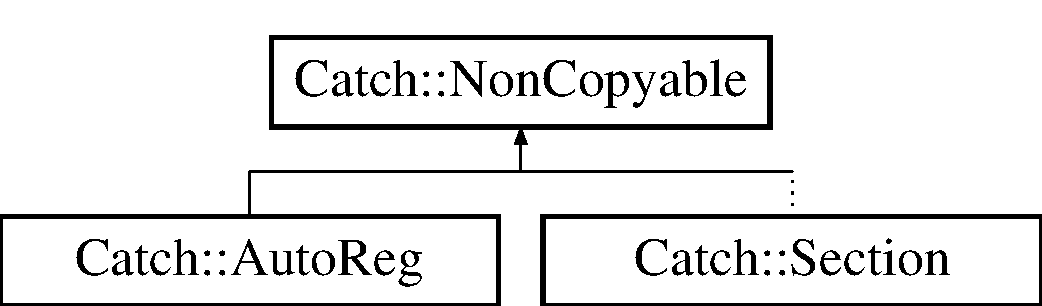
\includegraphics[height=2.000000cm]{class_catch_1_1_non_copyable}
\end{center}
\end{figure}


The documentation for this class was generated from the following file\+:\begin{DoxyCompactItemize}
\item 
catch.\+hpp\end{DoxyCompactItemize}

\hypertarget{struct_catch_1_1not__this__one}{}\section{Catch\+:\+:not\+\_\+this\+\_\+one Struct Reference}
\label{struct_catch_1_1not__this__one}\index{Catch\+::not\+\_\+this\+\_\+one@{Catch\+::not\+\_\+this\+\_\+one}}


The documentation for this struct was generated from the following file\+:\begin{DoxyCompactItemize}
\item 
catch.\+hpp\end{DoxyCompactItemize}

\hypertarget{struct_catch_1_1_generators_1_1_null_generator}{}\section{Catch\+:\+:Generators\+:\+:Null\+Generator$<$ T $>$ Struct Template Reference}
\label{struct_catch_1_1_generators_1_1_null_generator}\index{Catch\+::\+Generators\+::\+Null\+Generator$<$ T $>$@{Catch\+::\+Generators\+::\+Null\+Generator$<$ T $>$}}
Inheritance diagram for Catch\+:\+:Generators\+:\+:Null\+Generator$<$ T $>$\+:\begin{figure}[H]
\begin{center}
\leavevmode
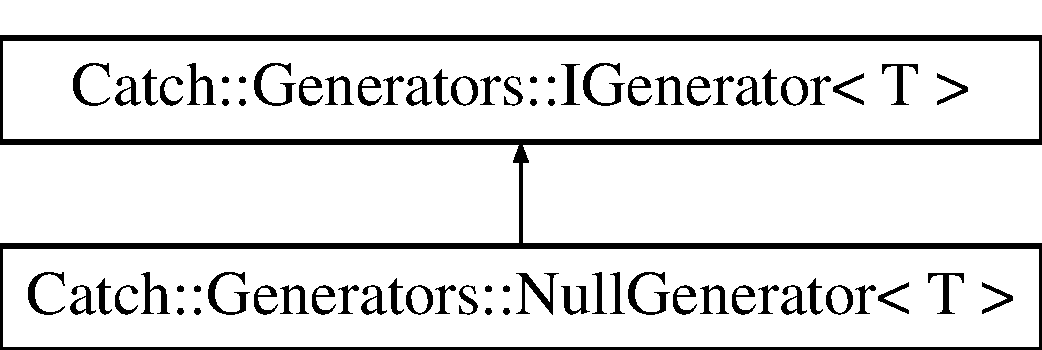
\includegraphics[height=2.000000cm]{struct_catch_1_1_generators_1_1_null_generator}
\end{center}
\end{figure}
\subsection*{Public Member Functions}
\begin{DoxyCompactItemize}
\item 
\mbox{\Hypertarget{struct_catch_1_1_generators_1_1_null_generator_a17a2cc82d644e97afded4017c7a062ef}\label{struct_catch_1_1_generators_1_1_null_generator_a17a2cc82d644e97afded4017c7a062ef}} 
auto {\bfseries get} (size\+\_\+t) const -\/$>$ T override
\end{DoxyCompactItemize}


The documentation for this struct was generated from the following file\+:\begin{DoxyCompactItemize}
\item 
catch.\+hpp\end{DoxyCompactItemize}

\hypertarget{class_aron_geometry_1_1_pair}{}\section{Aron\+Geometry\+:\+:Pair$<$ T $>$ Class Template Reference}
\label{class_aron_geometry_1_1_pair}\index{Aron\+Geometry\+::\+Pair$<$ T $>$@{Aron\+Geometry\+::\+Pair$<$ T $>$}}
\subsection*{Public Member Functions}
\begin{DoxyCompactItemize}
\item 
\mbox{\Hypertarget{class_aron_geometry_1_1_pair_a80516e37ec697f52990a300763d23e99}\label{class_aron_geometry_1_1_pair_a80516e37ec697f52990a300763d23e99}} 
{\bfseries Pair} (\mbox{\hyperlink{class_aron_geometry_1_1_point}{Point}}$<$ T $>$ p0, \mbox{\hyperlink{class_aron_geometry_1_1_point}{Point}}$<$ T $>$ p1)
\item 
\mbox{\Hypertarget{class_aron_geometry_1_1_pair_a05da2787bf15b098347e4c607159534b}\label{class_aron_geometry_1_1_pair_a05da2787bf15b098347e4c607159534b}} 
\mbox{\hyperlink{class_aron_geometry_1_1_pair}{Pair}} {\bfseries operator+} (\mbox{\hyperlink{class_aron_geometry_1_1_pair}{Pair}} pair)
\item 
\mbox{\Hypertarget{class_aron_geometry_1_1_pair_a28541db6d38c0512add73570085443c3}\label{class_aron_geometry_1_1_pair_a28541db6d38c0512add73570085443c3}} 
\mbox{\hyperlink{class_aron_geometry_1_1_pair}{Pair}} {\bfseries operator-\/} (\mbox{\hyperlink{class_aron_geometry_1_1_pair}{Pair}} pair)
\end{DoxyCompactItemize}
\subsection*{Public Attributes}
\begin{DoxyCompactItemize}
\item 
\mbox{\Hypertarget{class_aron_geometry_1_1_pair_adc3d8337ca7d79e106cf451a9d17bfe2}\label{class_aron_geometry_1_1_pair_adc3d8337ca7d79e106cf451a9d17bfe2}} 
\mbox{\hyperlink{class_aron_geometry_1_1_point}{Point}}$<$ T $>$ {\bfseries p0}
\item 
\mbox{\Hypertarget{class_aron_geometry_1_1_pair_acc8fd3291f807adc21c5f8bdc35d96db}\label{class_aron_geometry_1_1_pair_acc8fd3291f807adc21c5f8bdc35d96db}} 
\mbox{\hyperlink{class_aron_geometry_1_1_point}{Point}}$<$ T $>$ {\bfseries p1}
\end{DoxyCompactItemize}


The documentation for this class was generated from the following file\+:\begin{DoxyCompactItemize}
\item 
Aron\+Lib.\+h\end{DoxyCompactItemize}

\hypertarget{class_parabola}{}\section{Parabola Class Reference}
\label{class_parabola}\index{Parabola@{Parabola}}
\subsection*{Public Member Functions}
\begin{DoxyCompactItemize}
\item 
\mbox{\Hypertarget{class_parabola_a70249ceb2366e800b83335a07cf19c4f}\label{class_parabola_a70249ceb2366e800b83335a07cf19c4f}} 
{\bfseries Parabola} (G\+Lfloat cx, G\+Lfloat cy, G\+Lfloat cz)
\item 
\mbox{\Hypertarget{class_parabola_a9d1785d6e230e7bb8d47989fd812dad6}\label{class_parabola_a9d1785d6e230e7bb8d47989fd812dad6}} 
void {\bfseries init} ()
\item 
\mbox{\Hypertarget{class_parabola_ae2b8e3448ce58a0ec6e8a0c940751230}\label{class_parabola_ae2b8e3448ce58a0ec6e8a0c940751230}} 
void {\bfseries draw} ()
\end{DoxyCompactItemize}
\subsection*{Public Attributes}
\begin{DoxyCompactItemize}
\item 
\mbox{\Hypertarget{class_parabola_a8b0796be982e29910afd5d4621e688f8}\label{class_parabola_a8b0796be982e29910afd5d4621e688f8}} 
G\+Lfloat {\bfseries x0} = 0.\+0
\item 
\mbox{\Hypertarget{class_parabola_a4d1873ce27306f7fc2ca3f7ea581bd77}\label{class_parabola_a4d1873ce27306f7fc2ca3f7ea581bd77}} 
G\+Lfloat {\bfseries y0} = 0.\+0
\item 
\mbox{\Hypertarget{class_parabola_a5b25f72d1baaabc25f94108665052a98}\label{class_parabola_a5b25f72d1baaabc25f94108665052a98}} 
G\+Lfloat {\bfseries z0} = 0.\+0
\item 
\mbox{\Hypertarget{class_parabola_a10032698d1a003969979ae52ce25f907}\label{class_parabola_a10032698d1a003969979ae52ce25f907}} 
G\+Lfloat {\bfseries x1} = 0.\+0
\item 
\mbox{\Hypertarget{class_parabola_acd479351bec2260b6d77a581daf10948}\label{class_parabola_acd479351bec2260b6d77a581daf10948}} 
G\+Lfloat {\bfseries y1} = 0.\+0
\item 
\mbox{\Hypertarget{class_parabola_ae987f29da3825769c8bcfa1001b7980a}\label{class_parabola_ae987f29da3825769c8bcfa1001b7980a}} 
G\+Lfloat {\bfseries z1} = 0.\+0
\item 
\mbox{\Hypertarget{class_parabola_a01072566a5ab65464cc421bb43113a5b}\label{class_parabola_a01072566a5ab65464cc421bb43113a5b}} 
G\+Lfloat {\bfseries cx} = 0.\+0
\item 
\mbox{\Hypertarget{class_parabola_aa74168de12a1d4a510339cbe3c6d8740}\label{class_parabola_aa74168de12a1d4a510339cbe3c6d8740}} 
G\+Lfloat {\bfseries cy} = 0.\+0
\item 
\mbox{\Hypertarget{class_parabola_a10ff03776abe8f4f2a3734f0b00f0b3d}\label{class_parabola_a10ff03776abe8f4f2a3734f0b00f0b3d}} 
G\+Lfloat {\bfseries cz} = 0.\+0
\end{DoxyCompactItemize}


The documentation for this class was generated from the following file\+:\begin{DoxyCompactItemize}
\item 
Parabola.\+h\end{DoxyCompactItemize}

\hypertarget{struct_catch_1_1pluralise}{}\section{Catch\+:\+:pluralise Struct Reference}
\label{struct_catch_1_1pluralise}\index{Catch\+::pluralise@{Catch\+::pluralise}}
\subsection*{Public Member Functions}
\begin{DoxyCompactItemize}
\item 
\mbox{\Hypertarget{struct_catch_1_1pluralise_a5c55e22de2416cfe416edf715c6b9234}\label{struct_catch_1_1pluralise_a5c55e22de2416cfe416edf715c6b9234}} 
{\bfseries pluralise} (std\+::size\+\_\+t count, std\+::string const \&label)
\end{DoxyCompactItemize}
\subsection*{Public Attributes}
\begin{DoxyCompactItemize}
\item 
\mbox{\Hypertarget{struct_catch_1_1pluralise_a4dce2fa13ec6f00fac09b2418265441e}\label{struct_catch_1_1pluralise_a4dce2fa13ec6f00fac09b2418265441e}} 
std\+::size\+\_\+t {\bfseries m\+\_\+count}
\item 
\mbox{\Hypertarget{struct_catch_1_1pluralise_a8849cbdd3f11ebe7747597c8644e8793}\label{struct_catch_1_1pluralise_a8849cbdd3f11ebe7747597c8644e8793}} 
std\+::string {\bfseries m\+\_\+label}
\end{DoxyCompactItemize}
\subsection*{Friends}
\begin{DoxyCompactItemize}
\item 
\mbox{\Hypertarget{struct_catch_1_1pluralise_aa7dac6b165514c1f85e0695d678fdef5}\label{struct_catch_1_1pluralise_aa7dac6b165514c1f85e0695d678fdef5}} 
std\+::ostream \& {\bfseries operator$<$$<$} (std\+::ostream \&os, \mbox{\hyperlink{struct_catch_1_1pluralise}{pluralise}} const \&pluraliser)
\end{DoxyCompactItemize}


The documentation for this struct was generated from the following file\+:\begin{DoxyCompactItemize}
\item 
catch.\+hpp\end{DoxyCompactItemize}

\hypertarget{class_aron_geometry_1_1_point}{}\section{Aron\+Geometry\+:\+:Point$<$ T $>$ Class Template Reference}
\label{class_aron_geometry_1_1_point}\index{Aron\+Geometry\+::\+Point$<$ T $>$@{Aron\+Geometry\+::\+Point$<$ T $>$}}
\subsection*{Public Member Functions}
\begin{DoxyCompactItemize}
\item 
\mbox{\Hypertarget{class_aron_geometry_1_1_point_a3438f57e0995c529fef23321deeff8f1}\label{class_aron_geometry_1_1_point_a3438f57e0995c529fef23321deeff8f1}} 
{\bfseries Point} (T x, T y, T z=0.\+0)
\item 
\mbox{\Hypertarget{class_aron_geometry_1_1_point_adc8d81988b0f019ca97f59b06beb3a20}\label{class_aron_geometry_1_1_point_adc8d81988b0f019ca97f59b06beb3a20}} 
\mbox{\hyperlink{class_aron_geometry_1_1_point}{Point}}$<$ T $>$ {\bfseries operator+} (\mbox{\hyperlink{class_aron_geometry_1_1_vector}{Vector}}$<$ T $>$ v)
\item 
\mbox{\Hypertarget{class_aron_geometry_1_1_point_a78428a1f9cb6f510cc487aa285d89329}\label{class_aron_geometry_1_1_point_a78428a1f9cb6f510cc487aa285d89329}} 
bool {\bfseries operator==} (\mbox{\hyperlink{class_aron_geometry_1_1_point}{Point}} p0)
\item 
\mbox{\Hypertarget{class_aron_geometry_1_1_point_a9a35912258a4231d577d737806dab5ee}\label{class_aron_geometry_1_1_point_a9a35912258a4231d577d737806dab5ee}} 
bool {\bfseries operator!=} (\mbox{\hyperlink{class_aron_geometry_1_1_point}{Point}} p0)
\end{DoxyCompactItemize}
\subsection*{Public Attributes}
\begin{DoxyCompactItemize}
\item 
\mbox{\Hypertarget{class_aron_geometry_1_1_point_a67828202f48623460d22f9180ba3ee7c}\label{class_aron_geometry_1_1_point_a67828202f48623460d22f9180ba3ee7c}} 
T {\bfseries x}
\item 
\mbox{\Hypertarget{class_aron_geometry_1_1_point_acd404e059ee2b5e379c52706754ba183}\label{class_aron_geometry_1_1_point_acd404e059ee2b5e379c52706754ba183}} 
T {\bfseries y}
\item 
\mbox{\Hypertarget{class_aron_geometry_1_1_point_a918a20d03ad9f09c6992863f204bd4eb}\label{class_aron_geometry_1_1_point_a918a20d03ad9f09c6992863f204bd4eb}} 
T {\bfseries z}
\end{DoxyCompactItemize}
\subsection*{Friends}
\begin{DoxyCompactItemize}
\item 
\mbox{\Hypertarget{class_aron_geometry_1_1_point_ab43d6e907fd4ee20a55af8313448af2c}\label{class_aron_geometry_1_1_point_ab43d6e907fd4ee20a55af8313448af2c}} 
\mbox{\hyperlink{class_aron_geometry_1_1_point}{Point}}$<$ T $>$ {\bfseries operator+} (\mbox{\hyperlink{class_aron_geometry_1_1_point}{Point}}$<$ T $>$ p1, \mbox{\hyperlink{class_aron_geometry_1_1_point}{Point}}$<$ T $>$ p2)
\item 
\mbox{\Hypertarget{class_aron_geometry_1_1_point_a879c4a6d2de9eb55c1ccf7631c81cec6}\label{class_aron_geometry_1_1_point_a879c4a6d2de9eb55c1ccf7631c81cec6}} 
\mbox{\hyperlink{class_aron_geometry_1_1_point}{Point}}$<$ T $>$ {\bfseries operator-\/} (\mbox{\hyperlink{class_aron_geometry_1_1_point}{Point}}$<$ T $>$ p1, \mbox{\hyperlink{class_aron_geometry_1_1_point}{Point}}$<$ T $>$ p2)
\item 
\mbox{\Hypertarget{class_aron_geometry_1_1_point_aa2485a1951c87ed829b6c28ea21502db}\label{class_aron_geometry_1_1_point_aa2485a1951c87ed829b6c28ea21502db}} 
\mbox{\hyperlink{class_aron_geometry_1_1_point}{Point}}$<$ T $>$ {\bfseries operator$\ast$} (double k, \mbox{\hyperlink{class_aron_geometry_1_1_point}{Point}}$<$ T $>$ p)
\item 
\mbox{\Hypertarget{class_aron_geometry_1_1_point_a7ebb94c5729750ad809bd96eece4eba8}\label{class_aron_geometry_1_1_point_a7ebb94c5729750ad809bd96eece4eba8}} 
\mbox{\hyperlink{class_aron_geometry_1_1_point}{Point}}$<$ T $>$ {\bfseries operator$\ast$} (\mbox{\hyperlink{class_aron_geometry_1_1_point}{Point}}$<$ T $>$ p, double k)
\end{DoxyCompactItemize}


The documentation for this class was generated from the following file\+:\begin{DoxyCompactItemize}
\item 
Aron\+Lib.\+h\end{DoxyCompactItemize}

\hypertarget{class_catch_1_1_matchers_1_1_generic_1_1_predicate_matcher}{}\section{Catch\+:\+:Matchers\+:\+:Generic\+:\+:Predicate\+Matcher$<$ T $>$ Class Template Reference}
\label{class_catch_1_1_matchers_1_1_generic_1_1_predicate_matcher}\index{Catch\+::\+Matchers\+::\+Generic\+::\+Predicate\+Matcher$<$ T $>$@{Catch\+::\+Matchers\+::\+Generic\+::\+Predicate\+Matcher$<$ T $>$}}
Inheritance diagram for Catch\+:\+:Matchers\+:\+:Generic\+:\+:Predicate\+Matcher$<$ T $>$\+:\begin{figure}[H]
\begin{center}
\leavevmode
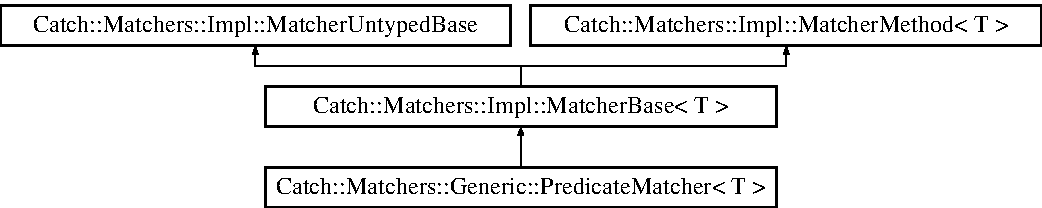
\includegraphics[height=2.790698cm]{class_catch_1_1_matchers_1_1_generic_1_1_predicate_matcher}
\end{center}
\end{figure}
\subsection*{Public Member Functions}
\begin{DoxyCompactItemize}
\item 
\mbox{\Hypertarget{class_catch_1_1_matchers_1_1_generic_1_1_predicate_matcher_a57d53ef028c2f7b92b016f627f91aa76}\label{class_catch_1_1_matchers_1_1_generic_1_1_predicate_matcher_a57d53ef028c2f7b92b016f627f91aa76}} 
{\bfseries Predicate\+Matcher} (std\+::function$<$ bool(T const \&)$>$ const \&elem, std\+::string const \&descr)
\item 
\mbox{\Hypertarget{class_catch_1_1_matchers_1_1_generic_1_1_predicate_matcher_a2ec0e8ec19c4c5e26271d59a06a62b52}\label{class_catch_1_1_matchers_1_1_generic_1_1_predicate_matcher_a2ec0e8ec19c4c5e26271d59a06a62b52}} 
bool {\bfseries match} (T const \&item) const override
\item 
\mbox{\Hypertarget{class_catch_1_1_matchers_1_1_generic_1_1_predicate_matcher_af7d59e94892cc09471bbaefac4c889fd}\label{class_catch_1_1_matchers_1_1_generic_1_1_predicate_matcher_af7d59e94892cc09471bbaefac4c889fd}} 
std\+::string {\bfseries describe} () const override
\end{DoxyCompactItemize}
\subsection*{Additional Inherited Members}


The documentation for this class was generated from the following file\+:\begin{DoxyCompactItemize}
\item 
catch.\+hpp\end{DoxyCompactItemize}

\hypertarget{class_catch_1_1_generators_1_1_range_generator}{}\section{Catch\+:\+:Generators\+:\+:Range\+Generator$<$ T $>$ Class Template Reference}
\label{class_catch_1_1_generators_1_1_range_generator}\index{Catch\+::\+Generators\+::\+Range\+Generator$<$ T $>$@{Catch\+::\+Generators\+::\+Range\+Generator$<$ T $>$}}
Inheritance diagram for Catch\+:\+:Generators\+:\+:Range\+Generator$<$ T $>$\+:\begin{figure}[H]
\begin{center}
\leavevmode
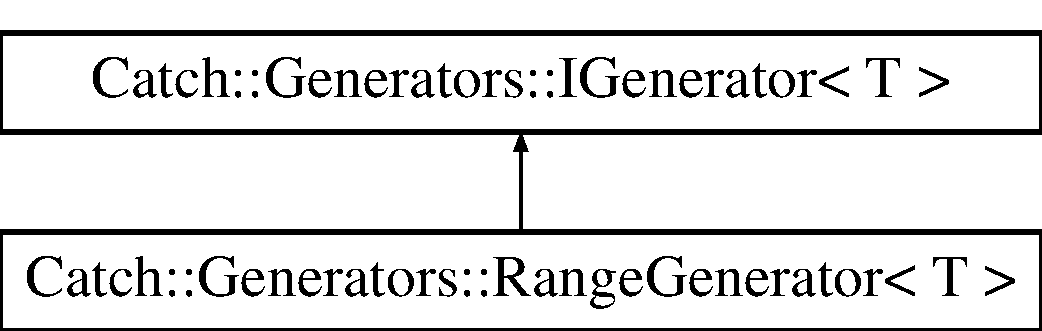
\includegraphics[height=2.000000cm]{class_catch_1_1_generators_1_1_range_generator}
\end{center}
\end{figure}
\subsection*{Public Member Functions}
\begin{DoxyCompactItemize}
\item 
\mbox{\Hypertarget{class_catch_1_1_generators_1_1_range_generator_a56c5fcc855bdb668d7b93c2017a7c44c}\label{class_catch_1_1_generators_1_1_range_generator_a56c5fcc855bdb668d7b93c2017a7c44c}} 
{\bfseries Range\+Generator} (T const \&first, T const \&last)
\item 
\mbox{\Hypertarget{class_catch_1_1_generators_1_1_range_generator_a78f7f624b7545823d1a683ebf2ac00e7}\label{class_catch_1_1_generators_1_1_range_generator_a78f7f624b7545823d1a683ebf2ac00e7}} 
auto {\bfseries get} (size\+\_\+t index) const -\/$>$ T override
\end{DoxyCompactItemize}


The documentation for this class was generated from the following file\+:\begin{DoxyCompactItemize}
\item 
catch.\+hpp\end{DoxyCompactItemize}

\hypertarget{struct_catch_1_1_matchers_1_1_std_string_1_1_regex_matcher}{}\section{Catch\+:\+:Matchers\+:\+:Std\+String\+:\+:Regex\+Matcher Struct Reference}
\label{struct_catch_1_1_matchers_1_1_std_string_1_1_regex_matcher}\index{Catch\+::\+Matchers\+::\+Std\+String\+::\+Regex\+Matcher@{Catch\+::\+Matchers\+::\+Std\+String\+::\+Regex\+Matcher}}
Inheritance diagram for Catch\+:\+:Matchers\+:\+:Std\+String\+:\+:Regex\+Matcher\+:\begin{figure}[H]
\begin{center}
\leavevmode
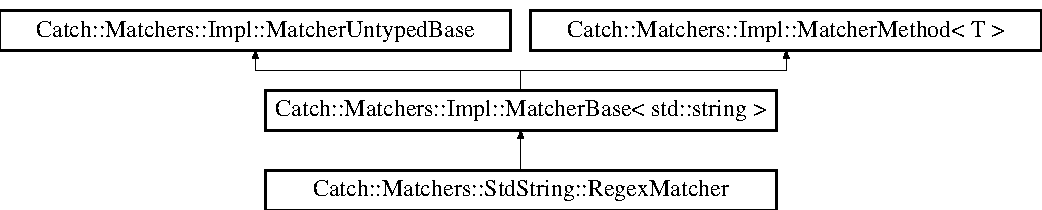
\includegraphics[height=2.818792cm]{struct_catch_1_1_matchers_1_1_std_string_1_1_regex_matcher}
\end{center}
\end{figure}
\subsection*{Public Member Functions}
\begin{DoxyCompactItemize}
\item 
\mbox{\Hypertarget{struct_catch_1_1_matchers_1_1_std_string_1_1_regex_matcher_ab914deb885fe25558c41ab368c6b3916}\label{struct_catch_1_1_matchers_1_1_std_string_1_1_regex_matcher_ab914deb885fe25558c41ab368c6b3916}} 
{\bfseries Regex\+Matcher} (std\+::string regex, Case\+Sensitive\+::\+Choice case\+Sensitivity)
\item 
\mbox{\Hypertarget{struct_catch_1_1_matchers_1_1_std_string_1_1_regex_matcher_aa8e61adccabb2f36133029301f6b8f4e}\label{struct_catch_1_1_matchers_1_1_std_string_1_1_regex_matcher_aa8e61adccabb2f36133029301f6b8f4e}} 
bool {\bfseries match} (std\+::string const \&matchee) const override
\item 
\mbox{\Hypertarget{struct_catch_1_1_matchers_1_1_std_string_1_1_regex_matcher_a1f788cd5258c987e5043f6c7f43adeb9}\label{struct_catch_1_1_matchers_1_1_std_string_1_1_regex_matcher_a1f788cd5258c987e5043f6c7f43adeb9}} 
std\+::string {\bfseries describe} () const override
\end{DoxyCompactItemize}
\subsection*{Additional Inherited Members}


The documentation for this struct was generated from the following file\+:\begin{DoxyCompactItemize}
\item 
catch.\+hpp\end{DoxyCompactItemize}

\hypertarget{struct_catch_1_1_registrar_for_tag_aliases}{}\section{Catch\+:\+:Registrar\+For\+Tag\+Aliases Struct Reference}
\label{struct_catch_1_1_registrar_for_tag_aliases}\index{Catch\+::\+Registrar\+For\+Tag\+Aliases@{Catch\+::\+Registrar\+For\+Tag\+Aliases}}
\subsection*{Public Member Functions}
\begin{DoxyCompactItemize}
\item 
\mbox{\Hypertarget{struct_catch_1_1_registrar_for_tag_aliases_ae4e45830e4763bcd65d55d8db9167b69}\label{struct_catch_1_1_registrar_for_tag_aliases_ae4e45830e4763bcd65d55d8db9167b69}} 
{\bfseries Registrar\+For\+Tag\+Aliases} (char const $\ast$alias, char const $\ast$tag, \mbox{\hyperlink{struct_catch_1_1_source_line_info}{Source\+Line\+Info}} const \&line\+Info)
\end{DoxyCompactItemize}


The documentation for this struct was generated from the following file\+:\begin{DoxyCompactItemize}
\item 
catch.\+hpp\end{DoxyCompactItemize}

\hypertarget{struct_catch_1_1_generators_1_1_requires_a_specialisation_for}{}\section{Catch\+:\+:Generators\+:\+:Requires\+A\+Specialisation\+For$<$ T $>$ Struct Template Reference}
\label{struct_catch_1_1_generators_1_1_requires_a_specialisation_for}\index{Catch\+::\+Generators\+::\+Requires\+A\+Specialisation\+For$<$ T $>$@{Catch\+::\+Generators\+::\+Requires\+A\+Specialisation\+For$<$ T $>$}}


The documentation for this struct was generated from the following file\+:\begin{DoxyCompactItemize}
\item 
catch.\+hpp\end{DoxyCompactItemize}

\hypertarget{struct_catch_1_1_result_disposition}{}\section{Catch\+:\+:Result\+Disposition Struct Reference}
\label{struct_catch_1_1_result_disposition}\index{Catch\+::\+Result\+Disposition@{Catch\+::\+Result\+Disposition}}
\subsection*{Public Types}
\begin{DoxyCompactItemize}
\item 
\mbox{\Hypertarget{struct_catch_1_1_result_disposition_a3396cad6e2259af326b3aae93e23e9d8}\label{struct_catch_1_1_result_disposition_a3396cad6e2259af326b3aae93e23e9d8}} 
enum {\bfseries Flags} \{ {\bfseries Normal} = 0x01, 
{\bfseries Continue\+On\+Failure} = 0x02, 
{\bfseries False\+Test} = 0x04, 
{\bfseries Suppress\+Fail} = 0x08
 \}
\end{DoxyCompactItemize}


The documentation for this struct was generated from the following file\+:\begin{DoxyCompactItemize}
\item 
catch.\+hpp\end{DoxyCompactItemize}

\hypertarget{struct_catch_1_1_result_was}{}\section{Catch\+:\+:Result\+Was Struct Reference}
\label{struct_catch_1_1_result_was}\index{Catch\+::\+Result\+Was@{Catch\+::\+Result\+Was}}
\subsection*{Public Types}
\begin{DoxyCompactItemize}
\item 
\mbox{\Hypertarget{struct_catch_1_1_result_was_a624e1ee3661fcf6094ceef1f654601ef}\label{struct_catch_1_1_result_was_a624e1ee3661fcf6094ceef1f654601ef}} 
enum {\bfseries Of\+Type} \{ \newline
{\bfseries Unknown} = -\/1, 
{\bfseries Ok} = 0, 
{\bfseries Info} = 1, 
{\bfseries Warning} = 2, 
\newline
{\bfseries Failure\+Bit} = 0x10, 
{\bfseries Expression\+Failed} = Failure\+Bit $\vert$ 1, 
{\bfseries Explicit\+Failure} = Failure\+Bit $\vert$ 2, 
{\bfseries Exception} = 0x100 $\vert$ Failure\+Bit, 
\newline
{\bfseries Threw\+Exception} = Exception $\vert$ 1, 
{\bfseries Didnt\+Throw\+Exception} = Exception $\vert$ 2, 
{\bfseries Fatal\+Error\+Condition} = 0x200 $\vert$ Failure\+Bit
 \}
\end{DoxyCompactItemize}


The documentation for this struct was generated from the following file\+:\begin{DoxyCompactItemize}
\item 
catch.\+hpp\end{DoxyCompactItemize}

\hypertarget{class_catch_1_1_reusable_string_stream}{}\section{Catch\+:\+:Reusable\+String\+Stream Class Reference}
\label{class_catch_1_1_reusable_string_stream}\index{Catch\+::\+Reusable\+String\+Stream@{Catch\+::\+Reusable\+String\+Stream}}
\subsection*{Public Member Functions}
\begin{DoxyCompactItemize}
\item 
\mbox{\Hypertarget{class_catch_1_1_reusable_string_stream_a0e9ecf260b2a5d35f4886ef0d51f6270}\label{class_catch_1_1_reusable_string_stream_a0e9ecf260b2a5d35f4886ef0d51f6270}} 
auto {\bfseries str} () const -\/$>$ std\+::string
\item 
\mbox{\Hypertarget{class_catch_1_1_reusable_string_stream_af95f72024c082db70e5e50782e28e4f6}\label{class_catch_1_1_reusable_string_stream_af95f72024c082db70e5e50782e28e4f6}} 
{\footnotesize template$<$typename T $>$ }\\auto {\bfseries operator$<$$<$} (T const \&value) -\/$>$ \mbox{\hyperlink{class_catch_1_1_reusable_string_stream}{Reusable\+String\+Stream}} \&
\item 
\mbox{\Hypertarget{class_catch_1_1_reusable_string_stream_a6881808c60a080d4e24a0b81c94cbf67}\label{class_catch_1_1_reusable_string_stream_a6881808c60a080d4e24a0b81c94cbf67}} 
auto {\bfseries get} () -\/$>$ std\+::ostream \&
\end{DoxyCompactItemize}


The documentation for this class was generated from the following file\+:\begin{DoxyCompactItemize}
\item 
catch.\+hpp\end{DoxyCompactItemize}

\hypertarget{class_matrix_vector_1_1row}{}\section{Matrix\+Vector\+:\+:row Class Reference}
\label{class_matrix_vector_1_1row}\index{Matrix\+Vector\+::row@{Matrix\+Vector\+::row}}
\subsection*{Public Member Functions}
\begin{DoxyCompactItemize}
\item 
\mbox{\Hypertarget{class_matrix_vector_1_1row_a811db3ee69813172bb193d301892d6c8}\label{class_matrix_vector_1_1row_a811db3ee69813172bb193d301892d6c8}} 
\mbox{\hyperlink{class_matrix_vector_1_1vec}{vec}} {\bfseries tran} ()
\item 
\mbox{\Hypertarget{class_matrix_vector_1_1row_a3a6cd508c032453418dd65c0ad7b2d29}\label{class_matrix_vector_1_1row_a3a6cd508c032453418dd65c0ad7b2d29}} 
float {\bfseries dot} (\mbox{\hyperlink{class_matrix_vector_1_1vec}{vec}} \&r)
\item 
\mbox{\Hypertarget{class_matrix_vector_1_1row_a8ee864b19f9e2f7272091f486d85f252}\label{class_matrix_vector_1_1row_a8ee864b19f9e2f7272091f486d85f252}} 
{\bfseries row} (int col, int \mbox{\hyperlink{class_matrix_vector_1_1row}{row}})
\item 
\mbox{\Hypertarget{class_matrix_vector_1_1row_ab1d7f626736a16cdc8d3670657c75213}\label{class_matrix_vector_1_1row_ab1d7f626736a16cdc8d3670657c75213}} 
{\bfseries row} (const \mbox{\hyperlink{class_matrix_vector_1_1row}{row}} \&r)
\item 
\mbox{\Hypertarget{class_matrix_vector_1_1row_a0a103a7fe75a43b4f2db2ce65f45caf5}\label{class_matrix_vector_1_1row_a0a103a7fe75a43b4f2db2ce65f45caf5}} 
void {\bfseries create\+Row} (float $\ast$array, int len)
\item 
\mbox{\Hypertarget{class_matrix_vector_1_1row_a1548f087a756261bb8dce854ef6d5528}\label{class_matrix_vector_1_1row_a1548f087a756261bb8dce854ef6d5528}} 
bool {\bfseries operator==} (const \mbox{\hyperlink{class_matrix_vector_1_1row}{row}} \&v)
\item 
\mbox{\Hypertarget{class_matrix_vector_1_1row_a8ba978a55b253872f974ecc20b80027a}\label{class_matrix_vector_1_1row_a8ba978a55b253872f974ecc20b80027a}} 
\mbox{\hyperlink{class_matrix_vector_1_1row}{row}} {\bfseries operator=} (const \mbox{\hyperlink{class_matrix_vector_1_1row}{row}} \&r)
\item 
\mbox{\Hypertarget{class_matrix_vector_1_1row_a914ac19994185e97ee1f81e04d7b9f57}\label{class_matrix_vector_1_1row_a914ac19994185e97ee1f81e04d7b9f57}} 
float {\bfseries operator$\ast$} (\mbox{\hyperlink{class_matrix_vector_1_1vec}{vec}} \&v)
\item 
\mbox{\Hypertarget{class_matrix_vector_1_1row_a48b1c08f1e5633f012a90f1165830239}\label{class_matrix_vector_1_1row_a48b1c08f1e5633f012a90f1165830239}} 
\mbox{\hyperlink{class_matrix_vector_1_1row}{row}} {\bfseries operator+} (\mbox{\hyperlink{class_matrix_vector_1_1row}{row}} \&r)
\item 
\mbox{\Hypertarget{class_matrix_vector_1_1row_a52e6591a45962217ff4c9aa07d8abff0}\label{class_matrix_vector_1_1row_a52e6591a45962217ff4c9aa07d8abff0}} 
\mbox{\hyperlink{class_matrix_vector_1_1row}{row}} {\bfseries operator-\/} (\mbox{\hyperlink{class_matrix_vector_1_1row}{row}} \&r)
\item 
\mbox{\Hypertarget{class_matrix_vector_1_1row_acb782a00f3402ab648206e27605f6ff2}\label{class_matrix_vector_1_1row_acb782a00f3402ab648206e27605f6ff2}} 
\mbox{\hyperlink{class_matrix_vector_1_1row}{row}} {\bfseries operator/} (float f)
\end{DoxyCompactItemize}
\subsection*{Public Attributes}
\begin{DoxyCompactItemize}
\item 
\mbox{\Hypertarget{class_matrix_vector_1_1row_afee52d0d3ef890b29f1e44f51cd71eca}\label{class_matrix_vector_1_1row_afee52d0d3ef890b29f1e44f51cd71eca}} 
int {\bfseries ncol}
\item 
\mbox{\Hypertarget{class_matrix_vector_1_1row_a999bc8b53ca12fa416f13aecb7d7e5a0}\label{class_matrix_vector_1_1row_a999bc8b53ca12fa416f13aecb7d7e5a0}} 
int {\bfseries nrow}
\item 
\mbox{\Hypertarget{class_matrix_vector_1_1row_af5d001ccb56241b693cd3d1cdf27992c}\label{class_matrix_vector_1_1row_af5d001ccb56241b693cd3d1cdf27992c}} 
float $\ast$$\ast$ {\bfseries arr}
\end{DoxyCompactItemize}


The documentation for this class was generated from the following file\+:\begin{DoxyCompactItemize}
\item 
Aron\+Lib.\+h\end{DoxyCompactItemize}

\hypertarget{class_catch_1_1_scoped_message}{}\section{Catch\+:\+:Scoped\+Message Class Reference}
\label{class_catch_1_1_scoped_message}\index{Catch\+::\+Scoped\+Message@{Catch\+::\+Scoped\+Message}}
\subsection*{Public Member Functions}
\begin{DoxyCompactItemize}
\item 
\mbox{\Hypertarget{class_catch_1_1_scoped_message_a5cc59f0f2ebe840e6607f83004d49a17}\label{class_catch_1_1_scoped_message_a5cc59f0f2ebe840e6607f83004d49a17}} 
{\bfseries Scoped\+Message} (\mbox{\hyperlink{struct_catch_1_1_message_builder}{Message\+Builder}} const \&builder)
\end{DoxyCompactItemize}
\subsection*{Public Attributes}
\begin{DoxyCompactItemize}
\item 
\mbox{\Hypertarget{class_catch_1_1_scoped_message_ae6e1476f389cc6e1586f033b3747b27b}\label{class_catch_1_1_scoped_message_ae6e1476f389cc6e1586f033b3747b27b}} 
\mbox{\hyperlink{struct_catch_1_1_message_info}{Message\+Info}} {\bfseries m\+\_\+info}
\end{DoxyCompactItemize}


The documentation for this class was generated from the following file\+:\begin{DoxyCompactItemize}
\item 
catch.\+hpp\end{DoxyCompactItemize}

\hypertarget{class_catch_1_1_section}{}\section{Catch\+:\+:Section Class Reference}
\label{class_catch_1_1_section}\index{Catch\+::\+Section@{Catch\+::\+Section}}
Inheritance diagram for Catch\+:\+:Section\+:\begin{figure}[H]
\begin{center}
\leavevmode
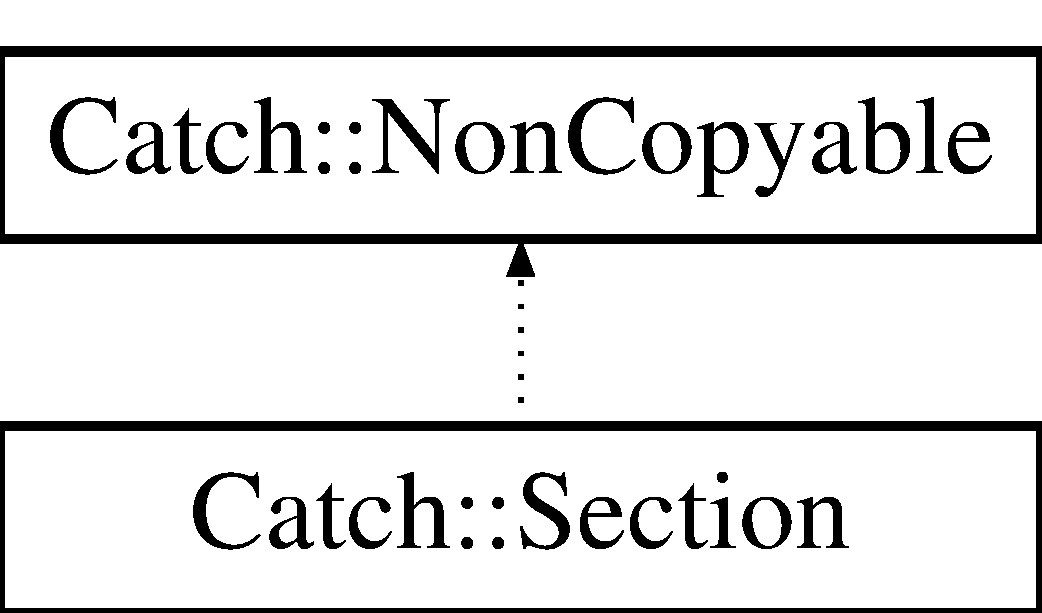
\includegraphics[height=2.000000cm]{class_catch_1_1_section}
\end{center}
\end{figure}
\subsection*{Public Member Functions}
\begin{DoxyCompactItemize}
\item 
\mbox{\Hypertarget{class_catch_1_1_section_a68fd4e51e8981aaa7ddb00d8a6abd099}\label{class_catch_1_1_section_a68fd4e51e8981aaa7ddb00d8a6abd099}} 
{\bfseries Section} (\mbox{\hyperlink{struct_catch_1_1_section_info}{Section\+Info}} const \&info)
\item 
\mbox{\Hypertarget{class_catch_1_1_section_a0632b804dcea1417a2970620a9742eb3}\label{class_catch_1_1_section_a0632b804dcea1417a2970620a9742eb3}} 
{\bfseries operator bool} () const
\end{DoxyCompactItemize}


The documentation for this class was generated from the following file\+:\begin{DoxyCompactItemize}
\item 
catch.\+hpp\end{DoxyCompactItemize}

\hypertarget{struct_catch_1_1_section_end_info}{}\section{Catch\+:\+:Section\+End\+Info Struct Reference}
\label{struct_catch_1_1_section_end_info}\index{Catch\+::\+Section\+End\+Info@{Catch\+::\+Section\+End\+Info}}
\subsection*{Public Attributes}
\begin{DoxyCompactItemize}
\item 
\mbox{\Hypertarget{struct_catch_1_1_section_end_info_a2d44793392cb83735d086d726822abe9}\label{struct_catch_1_1_section_end_info_a2d44793392cb83735d086d726822abe9}} 
\mbox{\hyperlink{struct_catch_1_1_section_info}{Section\+Info}} {\bfseries section\+Info}
\item 
\mbox{\Hypertarget{struct_catch_1_1_section_end_info_ae70b154cbc05b5dd2901d97f89303d8c}\label{struct_catch_1_1_section_end_info_ae70b154cbc05b5dd2901d97f89303d8c}} 
\mbox{\hyperlink{struct_catch_1_1_counts}{Counts}} {\bfseries prev\+Assertions}
\item 
\mbox{\Hypertarget{struct_catch_1_1_section_end_info_a7c262f2dab9cff166b8eca620c47eea5}\label{struct_catch_1_1_section_end_info_a7c262f2dab9cff166b8eca620c47eea5}} 
double {\bfseries duration\+In\+Seconds}
\end{DoxyCompactItemize}


The documentation for this struct was generated from the following file\+:\begin{DoxyCompactItemize}
\item 
catch.\+hpp\end{DoxyCompactItemize}

\hypertarget{struct_catch_1_1_section_info}{}\section{Catch\+:\+:Section\+Info Struct Reference}
\label{struct_catch_1_1_section_info}\index{Catch\+::\+Section\+Info@{Catch\+::\+Section\+Info}}
\subsection*{Public Member Functions}
\begin{DoxyCompactItemize}
\item 
\mbox{\Hypertarget{struct_catch_1_1_section_info_a2808437ae7d4bc0830cee1c3995165a6}\label{struct_catch_1_1_section_info_a2808437ae7d4bc0830cee1c3995165a6}} 
{\bfseries Section\+Info} (\mbox{\hyperlink{struct_catch_1_1_source_line_info}{Source\+Line\+Info}} const \&\+\_\+line\+Info, std\+::string const \&\+\_\+name)
\item 
\mbox{\Hypertarget{struct_catch_1_1_section_info_a139875f2e7bd12a5898a948f8bad15b3}\label{struct_catch_1_1_section_info_a139875f2e7bd12a5898a948f8bad15b3}} 
{\bfseries Section\+Info} (\mbox{\hyperlink{struct_catch_1_1_source_line_info}{Source\+Line\+Info}} const \&\+\_\+line\+Info, std\+::string const \&\+\_\+name, std\+::string const \&)
\end{DoxyCompactItemize}
\subsection*{Public Attributes}
\begin{DoxyCompactItemize}
\item 
\mbox{\Hypertarget{struct_catch_1_1_section_info_a704c8fc662d309137e0d4f199cb7df58}\label{struct_catch_1_1_section_info_a704c8fc662d309137e0d4f199cb7df58}} 
std\+::string {\bfseries name}
\item 
\mbox{\Hypertarget{struct_catch_1_1_section_info_a0052060219a6de74bb7ade34d4163a4e}\label{struct_catch_1_1_section_info_a0052060219a6de74bb7ade34d4163a4e}} 
std\+::string {\bfseries description}
\item 
\mbox{\Hypertarget{struct_catch_1_1_section_info_adbc83b8a3507c4acc8ee249e93465711}\label{struct_catch_1_1_section_info_adbc83b8a3507c4acc8ee249e93465711}} 
\mbox{\hyperlink{struct_catch_1_1_source_line_info}{Source\+Line\+Info}} {\bfseries line\+Info}
\end{DoxyCompactItemize}


The documentation for this struct was generated from the following file\+:\begin{DoxyCompactItemize}
\item 
catch.\+hpp\end{DoxyCompactItemize}

\hypertarget{class_aron_geometry_1_1_segment}{}\section{Aron\+Geometry\+:\+:Segment$<$ T $>$ Class Template Reference}
\label{class_aron_geometry_1_1_segment}\index{Aron\+Geometry\+::\+Segment$<$ T $>$@{Aron\+Geometry\+::\+Segment$<$ T $>$}}
\subsection*{Public Member Functions}
\begin{DoxyCompactItemize}
\item 
\mbox{\Hypertarget{class_aron_geometry_1_1_segment_a464f4f8dbe8950ef7c94fe170e1f3fce}\label{class_aron_geometry_1_1_segment_a464f4f8dbe8950ef7c94fe170e1f3fce}} 
{\bfseries Segment} (\mbox{\hyperlink{class_aron_geometry_1_1_point}{Point}}$<$ T $>$ p0, \mbox{\hyperlink{class_aron_geometry_1_1_point}{Point}}$<$ T $>$ p1)
\item 
\mbox{\Hypertarget{class_aron_geometry_1_1_segment_a476cb580ab1fc62df5bcb684aa9bcb6c}\label{class_aron_geometry_1_1_segment_a476cb580ab1fc62df5bcb684aa9bcb6c}} 
double {\bfseries square\+Dist} ()
\item 
\mbox{\Hypertarget{class_aron_geometry_1_1_segment_ad8a973579b4789e9d7e4f7f84b425334}\label{class_aron_geometry_1_1_segment_ad8a973579b4789e9d7e4f7f84b425334}} 
double {\bfseries distance} ()
\item 
\mbox{\Hypertarget{class_aron_geometry_1_1_segment_a9ff59835f5ad9edeef72003aecd1b649}\label{class_aron_geometry_1_1_segment_a9ff59835f5ad9edeef72003aecd1b649}} 
bool {\bfseries is\+Colinear} (\mbox{\hyperlink{class_aron_geometry_1_1_point}{Point}}$<$ T $>$ p)
\item 
\mbox{\Hypertarget{class_aron_geometry_1_1_segment_af46cd60cb68c4fd238e0feeb82bb08cb}\label{class_aron_geometry_1_1_segment_af46cd60cb68c4fd238e0feeb82bb08cb}} 
bool {\bfseries is\+Cross\+Segment} (\mbox{\hyperlink{class_aron_geometry_1_1_segment}{Segment}}$<$ T $>$ s1, \mbox{\hyperlink{class_aron_geometry_1_1_segment}{Segment}}$<$ T $>$ s2)
\item 
\mbox{\Hypertarget{class_aron_geometry_1_1_segment_a4318e5703dd1f408085df1e049dabf0b}\label{class_aron_geometry_1_1_segment_a4318e5703dd1f408085df1e049dabf0b}} 
bool {\bfseries is\+End\+Point} (\mbox{\hyperlink{class_aron_geometry_1_1_point}{Point}}$<$ T $>$ p)
\item 
\mbox{\Hypertarget{class_aron_geometry_1_1_segment_a3cb9fb71f3df833bf5a4959f2c514ab4}\label{class_aron_geometry_1_1_segment_a3cb9fb71f3df833bf5a4959f2c514ab4}} 
bool {\bfseries operator==} (\mbox{\hyperlink{class_aron_geometry_1_1_segment}{Segment}}$<$ T $>$ s)
\end{DoxyCompactItemize}
\subsection*{Public Attributes}
\begin{DoxyCompactItemize}
\item 
\mbox{\Hypertarget{class_aron_geometry_1_1_segment_a0339fdcab581818eca4c6319619026fa}\label{class_aron_geometry_1_1_segment_a0339fdcab581818eca4c6319619026fa}} 
\mbox{\hyperlink{class_aron_geometry_1_1_point}{Point}}$<$ T $>$ {\bfseries p0}
\item 
\mbox{\Hypertarget{class_aron_geometry_1_1_segment_ae38bb4aa1fca8e6ca664017c1dfd60bf}\label{class_aron_geometry_1_1_segment_ae38bb4aa1fca8e6ca664017c1dfd60bf}} 
\mbox{\hyperlink{class_aron_geometry_1_1_point}{Point}}$<$ T $>$ {\bfseries p1}
\end{DoxyCompactItemize}


The documentation for this class was generated from the following file\+:\begin{DoxyCompactItemize}
\item 
Aron\+Lib.\+h\end{DoxyCompactItemize}

\hypertarget{class_simple_coordinate}{}\section{Simple\+Coordinate Class Reference}
\label{class_simple_coordinate}\index{Simple\+Coordinate@{Simple\+Coordinate}}
\subsection*{Public Member Functions}
\begin{DoxyCompactItemize}
\item 
\mbox{\Hypertarget{class_simple_coordinate_aa3f1d2894a4a1f060f40bd8f3a9e3b91}\label{class_simple_coordinate_aa3f1d2894a4a1f060f40bd8f3a9e3b91}} 
void {\bfseries draw} (float width=1.\+0, int num=10)
\end{DoxyCompactItemize}


The documentation for this class was generated from the following file\+:\begin{DoxyCompactItemize}
\item 
Aron\+Open\+G\+L\+Lib.\+h\end{DoxyCompactItemize}

\hypertarget{class_catch_1_1_generators_1_1_single_value_generator}{}\section{Catch\+:\+:Generators\+:\+:Single\+Value\+Generator$<$ T $>$ Class Template Reference}
\label{class_catch_1_1_generators_1_1_single_value_generator}\index{Catch\+::\+Generators\+::\+Single\+Value\+Generator$<$ T $>$@{Catch\+::\+Generators\+::\+Single\+Value\+Generator$<$ T $>$}}
Inheritance diagram for Catch\+:\+:Generators\+:\+:Single\+Value\+Generator$<$ T $>$\+:\begin{figure}[H]
\begin{center}
\leavevmode
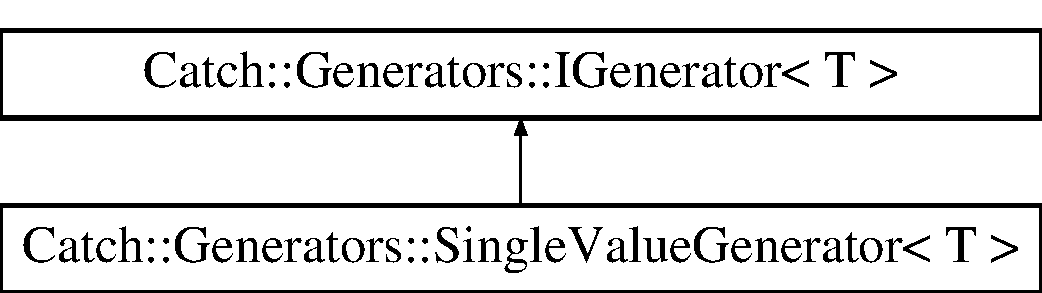
\includegraphics[height=2.000000cm]{class_catch_1_1_generators_1_1_single_value_generator}
\end{center}
\end{figure}
\subsection*{Public Member Functions}
\begin{DoxyCompactItemize}
\item 
\mbox{\Hypertarget{class_catch_1_1_generators_1_1_single_value_generator_a4bed2ad14ffe04102d8135e2c82b3ace}\label{class_catch_1_1_generators_1_1_single_value_generator_a4bed2ad14ffe04102d8135e2c82b3ace}} 
{\bfseries Single\+Value\+Generator} (T const \&value)
\item 
\mbox{\Hypertarget{class_catch_1_1_generators_1_1_single_value_generator_ad03af3fe263136425595bfd2eec84209}\label{class_catch_1_1_generators_1_1_single_value_generator_ad03af3fe263136425595bfd2eec84209}} 
auto {\bfseries get} (size\+\_\+t) const -\/$>$ T override
\end{DoxyCompactItemize}


The documentation for this class was generated from the following file\+:\begin{DoxyCompactItemize}
\item 
catch.\+hpp\end{DoxyCompactItemize}

\hypertarget{class_s_l_l}{}\section{S\+LL$<$ Type $>$ Class Template Reference}
\label{class_s_l_l}\index{S\+L\+L$<$ Type $>$@{S\+L\+L$<$ Type $>$}}
\subsection*{Public Member Functions}
\begin{DoxyCompactItemize}
\item 
\mbox{\Hypertarget{class_s_l_l_a4a183f28b712006ca9e6c86f7052cc39}\label{class_s_l_l_a4a183f28b712006ca9e6c86f7052cc39}} 
void {\bfseries append} (Type data)
\item 
\mbox{\Hypertarget{class_s_l_l_ac0745119053c511f59f5ffb50d99b3d7}\label{class_s_l_l_ac0745119053c511f59f5ffb50d99b3d7}} 
void {\bfseries append} (\mbox{\hyperlink{class_node}{Node}}$<$ Type $>$ $\ast$node)
\item 
\mbox{\Hypertarget{class_s_l_l_a251fa3c50d9fb5bb6247ce1dd9bd4a3d}\label{class_s_l_l_a251fa3c50d9fb5bb6247ce1dd9bd4a3d}} 
void {\bfseries print} ()
\item 
\mbox{\Hypertarget{class_s_l_l_a4e9e7161dfba0cea42fd2a805e4883df}\label{class_s_l_l_a4e9e7161dfba0cea42fd2a805e4883df}} 
int {\bfseries count} ()
\item 
\mbox{\Hypertarget{class_s_l_l_af0b39dec9cebd5991b992ae4cadff2ba}\label{class_s_l_l_af0b39dec9cebd5991b992ae4cadff2ba}} 
void {\bfseries remove} (Type item)
\item 
\mbox{\Hypertarget{class_s_l_l_a4da3d7fa252ba1e747da867977aeede8}\label{class_s_l_l_a4da3d7fa252ba1e747da867977aeede8}} 
void {\bfseries remove} (\mbox{\hyperlink{class_node}{Node}}$<$ Type $>$ $\ast$node)
\end{DoxyCompactItemize}
\subsection*{Public Attributes}
\begin{DoxyCompactItemize}
\item 
\mbox{\Hypertarget{class_s_l_l_a8fed5c8dc2b39042c515d1473119dadb}\label{class_s_l_l_a8fed5c8dc2b39042c515d1473119dadb}} 
\mbox{\hyperlink{class_node}{Node}}$<$ Type $>$ $\ast$ {\bfseries head}
\end{DoxyCompactItemize}


The documentation for this class was generated from the following file\+:\begin{DoxyCompactItemize}
\item 
S\+L\+L.\+h\end{DoxyCompactItemize}

\hypertarget{struct_catch_1_1_source_line_info}{}\section{Catch\+:\+:Source\+Line\+Info Struct Reference}
\label{struct_catch_1_1_source_line_info}\index{Catch\+::\+Source\+Line\+Info@{Catch\+::\+Source\+Line\+Info}}
\subsection*{Public Member Functions}
\begin{DoxyCompactItemize}
\item 
\mbox{\Hypertarget{struct_catch_1_1_source_line_info_a48510b82a39a042ab370ed143dd30c10}\label{struct_catch_1_1_source_line_info_a48510b82a39a042ab370ed143dd30c10}} 
{\bfseries Source\+Line\+Info} (char const $\ast$\+\_\+file, std\+::size\+\_\+t \+\_\+line) noexcept
\item 
\mbox{\Hypertarget{struct_catch_1_1_source_line_info_a7c44c9986c33a9cf842b791374332d41}\label{struct_catch_1_1_source_line_info_a7c44c9986c33a9cf842b791374332d41}} 
{\bfseries Source\+Line\+Info} (\mbox{\hyperlink{struct_catch_1_1_source_line_info}{Source\+Line\+Info}} const \&other)=default
\item 
\mbox{\Hypertarget{struct_catch_1_1_source_line_info_a6614b503b493bbdd3b49a1bd732e0a55}\label{struct_catch_1_1_source_line_info_a6614b503b493bbdd3b49a1bd732e0a55}} 
{\bfseries Source\+Line\+Info} (\mbox{\hyperlink{struct_catch_1_1_source_line_info}{Source\+Line\+Info}} \&\&)=default
\item 
\mbox{\Hypertarget{struct_catch_1_1_source_line_info_a1a6cfc0197357ef4e329bb256aa8a354}\label{struct_catch_1_1_source_line_info_a1a6cfc0197357ef4e329bb256aa8a354}} 
\mbox{\hyperlink{struct_catch_1_1_source_line_info}{Source\+Line\+Info}} \& {\bfseries operator=} (\mbox{\hyperlink{struct_catch_1_1_source_line_info}{Source\+Line\+Info}} const \&)=default
\item 
\mbox{\Hypertarget{struct_catch_1_1_source_line_info_a7fa35372f2bca5e91adc25327b7c753c}\label{struct_catch_1_1_source_line_info_a7fa35372f2bca5e91adc25327b7c753c}} 
\mbox{\hyperlink{struct_catch_1_1_source_line_info}{Source\+Line\+Info}} \& {\bfseries operator=} (\mbox{\hyperlink{struct_catch_1_1_source_line_info}{Source\+Line\+Info}} \&\&)=default
\item 
\mbox{\Hypertarget{struct_catch_1_1_source_line_info_a10a5b5b7dff82971879c2eb8d83f9b3b}\label{struct_catch_1_1_source_line_info_a10a5b5b7dff82971879c2eb8d83f9b3b}} 
bool {\bfseries empty} () const noexcept
\item 
\mbox{\Hypertarget{struct_catch_1_1_source_line_info_af07e4fdeddf8409b91e4f842f6264cf8}\label{struct_catch_1_1_source_line_info_af07e4fdeddf8409b91e4f842f6264cf8}} 
bool {\bfseries operator==} (\mbox{\hyperlink{struct_catch_1_1_source_line_info}{Source\+Line\+Info}} const \&other) const noexcept
\item 
\mbox{\Hypertarget{struct_catch_1_1_source_line_info_af77415416919d2d6030b4be085b92f7a}\label{struct_catch_1_1_source_line_info_af77415416919d2d6030b4be085b92f7a}} 
bool {\bfseries operator$<$} (\mbox{\hyperlink{struct_catch_1_1_source_line_info}{Source\+Line\+Info}} const \&other) const noexcept
\end{DoxyCompactItemize}
\subsection*{Public Attributes}
\begin{DoxyCompactItemize}
\item 
\mbox{\Hypertarget{struct_catch_1_1_source_line_info_ad65537703e9f08c1fa7777fbc3f0c617}\label{struct_catch_1_1_source_line_info_ad65537703e9f08c1fa7777fbc3f0c617}} 
char const  $\ast$ {\bfseries file}
\item 
\mbox{\Hypertarget{struct_catch_1_1_source_line_info_a841e5d696c7b9cde24e45e61dd979c77}\label{struct_catch_1_1_source_line_info_a841e5d696c7b9cde24e45e61dd979c77}} 
std\+::size\+\_\+t {\bfseries line}
\end{DoxyCompactItemize}


The documentation for this struct was generated from the following file\+:\begin{DoxyCompactItemize}
\item 
catch.\+hpp\end{DoxyCompactItemize}

\hypertarget{class_stack}{}\section{Stack$<$ Type $>$ Class Template Reference}
\label{class_stack}\index{Stack$<$ Type $>$@{Stack$<$ Type $>$}}
\subsection*{Public Member Functions}
\begin{DoxyCompactItemize}
\item 
\mbox{\Hypertarget{class_stack_a12509631738ba84ee426b2a204d4402a}\label{class_stack_a12509631738ba84ee426b2a204d4402a}} 
void {\bfseries push} (Type item)
\item 
\mbox{\Hypertarget{class_stack_ae712de8026eaaad433e4f1e016effabb}\label{class_stack_ae712de8026eaaad433e4f1e016effabb}} 
bool {\bfseries empty} ()
\item 
\mbox{\Hypertarget{class_stack_a2a8daadc1f221da7f7ceb87eb504f4f4}\label{class_stack_a2a8daadc1f221da7f7ceb87eb504f4f4}} 
int {\bfseries count} ()
\item 
\mbox{\Hypertarget{class_stack_ae8d94f9cabbf93bf0f940dee67e98b62}\label{class_stack_ae8d94f9cabbf93bf0f940dee67e98b62}} 
Type {\bfseries pop} ()
\end{DoxyCompactItemize}


The documentation for this class was generated from the following file\+:\begin{DoxyCompactItemize}
\item 
Stack.\+h\end{DoxyCompactItemize}

\hypertarget{struct_catch_1_1_matchers_1_1_std_string_1_1_starts_with_matcher}{}\section{Catch\+:\+:Matchers\+:\+:Std\+String\+:\+:Starts\+With\+Matcher Struct Reference}
\label{struct_catch_1_1_matchers_1_1_std_string_1_1_starts_with_matcher}\index{Catch\+::\+Matchers\+::\+Std\+String\+::\+Starts\+With\+Matcher@{Catch\+::\+Matchers\+::\+Std\+String\+::\+Starts\+With\+Matcher}}
Inheritance diagram for Catch\+:\+:Matchers\+:\+:Std\+String\+:\+:Starts\+With\+Matcher\+:\begin{figure}[H]
\begin{center}
\leavevmode
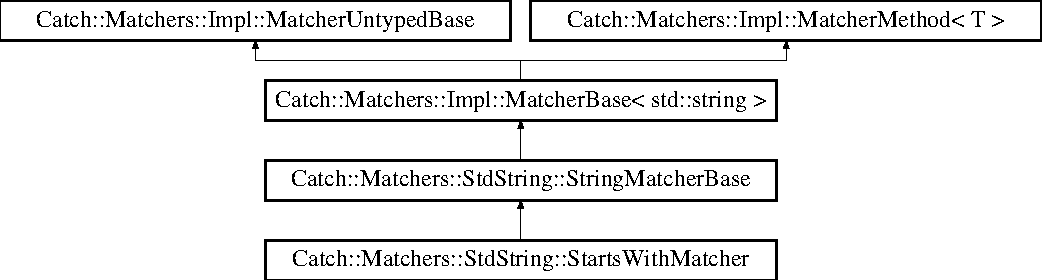
\includegraphics[height=3.758389cm]{struct_catch_1_1_matchers_1_1_std_string_1_1_starts_with_matcher}
\end{center}
\end{figure}
\subsection*{Public Member Functions}
\begin{DoxyCompactItemize}
\item 
\mbox{\Hypertarget{struct_catch_1_1_matchers_1_1_std_string_1_1_starts_with_matcher_a7b86f258bdbd131a6e7bcd94a8977325}\label{struct_catch_1_1_matchers_1_1_std_string_1_1_starts_with_matcher_a7b86f258bdbd131a6e7bcd94a8977325}} 
{\bfseries Starts\+With\+Matcher} (\mbox{\hyperlink{struct_catch_1_1_matchers_1_1_std_string_1_1_cased_string}{Cased\+String}} const \&comparator)
\item 
\mbox{\Hypertarget{struct_catch_1_1_matchers_1_1_std_string_1_1_starts_with_matcher_a7da4747aed0c48989d8be59a89e2b7fb}\label{struct_catch_1_1_matchers_1_1_std_string_1_1_starts_with_matcher_a7da4747aed0c48989d8be59a89e2b7fb}} 
bool {\bfseries match} (std\+::string const \&source) const override
\end{DoxyCompactItemize}
\subsection*{Additional Inherited Members}


The documentation for this struct was generated from the following file\+:\begin{DoxyCompactItemize}
\item 
catch.\+hpp\end{DoxyCompactItemize}

\hypertarget{class_stop_watch}{}\section{Stop\+Watch Class Reference}
\label{class_stop_watch}\index{Stop\+Watch@{Stop\+Watch}}
\subsection*{Public Member Functions}
\begin{DoxyCompactItemize}
\item 
\mbox{\Hypertarget{class_stop_watch_a0fb3ab295580a7d29d55ca52b41f6294}\label{class_stop_watch_a0fb3ab295580a7d29d55ca52b41f6294}} 
void {\bfseries begin} ()
\item 
\mbox{\Hypertarget{class_stop_watch_aea19465133bf92b9abfb7da79940c230}\label{class_stop_watch_aea19465133bf92b9abfb7da79940c230}} 
void {\bfseries end} ()
\item 
\mbox{\Hypertarget{class_stop_watch_a11cecbd5155cbd4076816ce24c43a337}\label{class_stop_watch_a11cecbd5155cbd4076816ce24c43a337}} 
void {\bfseries print} ()
\end{DoxyCompactItemize}


The documentation for this class was generated from the following file\+:\begin{DoxyCompactItemize}
\item 
Aron\+Lib.\+h\end{DoxyCompactItemize}

\hypertarget{struct_catch_1_1_stream_end_stop}{}\section{Catch\+:\+:Stream\+End\+Stop Struct Reference}
\label{struct_catch_1_1_stream_end_stop}\index{Catch\+::\+Stream\+End\+Stop@{Catch\+::\+Stream\+End\+Stop}}
\subsection*{Public Member Functions}
\begin{DoxyCompactItemize}
\item 
\mbox{\Hypertarget{struct_catch_1_1_stream_end_stop_a4a518f0342a381074821d5bda2651401}\label{struct_catch_1_1_stream_end_stop_a4a518f0342a381074821d5bda2651401}} 
std\+::string {\bfseries operator+} () const
\end{DoxyCompactItemize}


The documentation for this struct was generated from the following file\+:\begin{DoxyCompactItemize}
\item 
catch.\+hpp\end{DoxyCompactItemize}

\hypertarget{struct_catch_1_1_string_maker}{}\section{Catch\+:\+:String\+Maker$<$ T, typename $>$ Struct Template Reference}
\label{struct_catch_1_1_string_maker}\index{Catch\+::\+String\+Maker$<$ T, typename $>$@{Catch\+::\+String\+Maker$<$ T, typename $>$}}
\subsection*{Static Public Member Functions}
\begin{DoxyCompactItemize}
\item 
\mbox{\Hypertarget{struct_catch_1_1_string_maker_ab2c357e22b754802c4b1351257103eb6}\label{struct_catch_1_1_string_maker_ab2c357e22b754802c4b1351257103eb6}} 
{\footnotesize template$<$typename Fake  = T$>$ }\\static std\+::enable\+\_\+if$<$\+::\mbox{\hyperlink{class_catch_1_1_detail_1_1_is_stream_insertable}{Catch\+::\+Detail\+::\+Is\+Stream\+Insertable}}$<$ Fake $>$\+::value, std\+::string $>$\+::type {\bfseries convert} (const Fake \&value)
\item 
\mbox{\Hypertarget{struct_catch_1_1_string_maker_a68bb548de0e5ad364228b1ca3dd2f561}\label{struct_catch_1_1_string_maker_a68bb548de0e5ad364228b1ca3dd2f561}} 
{\footnotesize template$<$typename Fake  = T$>$ }\\static std\+::enable\+\_\+if$<$!\+::\mbox{\hyperlink{class_catch_1_1_detail_1_1_is_stream_insertable}{Catch\+::\+Detail\+::\+Is\+Stream\+Insertable}}$<$ Fake $>$\+::value, std\+::string $>$\+::type {\bfseries convert} (const Fake \&value)
\end{DoxyCompactItemize}


The documentation for this struct was generated from the following file\+:\begin{DoxyCompactItemize}
\item 
catch.\+hpp\end{DoxyCompactItemize}

\hypertarget{struct_catch_1_1_string_maker_3_01bool_01_4}{}\section{Catch\+:\+:String\+Maker$<$ bool $>$ Struct Template Reference}
\label{struct_catch_1_1_string_maker_3_01bool_01_4}\index{Catch\+::\+String\+Maker$<$ bool $>$@{Catch\+::\+String\+Maker$<$ bool $>$}}
\subsection*{Static Public Member Functions}
\begin{DoxyCompactItemize}
\item 
\mbox{\Hypertarget{struct_catch_1_1_string_maker_3_01bool_01_4_a37e9899c82c4b4515f876f16f8957a77}\label{struct_catch_1_1_string_maker_3_01bool_01_4_a37e9899c82c4b4515f876f16f8957a77}} 
static std\+::string {\bfseries convert} (bool b)
\end{DoxyCompactItemize}


The documentation for this struct was generated from the following file\+:\begin{DoxyCompactItemize}
\item 
catch.\+hpp\end{DoxyCompactItemize}

\hypertarget{struct_catch_1_1_string_maker_3_01_catch_1_1_detail_1_1_approx_01_4}{}\section{Catch\+:\+:String\+Maker$<$ Catch\+:\+:Detail\+:\+:Approx $>$ Struct Template Reference}
\label{struct_catch_1_1_string_maker_3_01_catch_1_1_detail_1_1_approx_01_4}\index{Catch\+::\+String\+Maker$<$ Catch\+::\+Detail\+::\+Approx $>$@{Catch\+::\+String\+Maker$<$ Catch\+::\+Detail\+::\+Approx $>$}}
\subsection*{Static Public Member Functions}
\begin{DoxyCompactItemize}
\item 
\mbox{\Hypertarget{struct_catch_1_1_string_maker_3_01_catch_1_1_detail_1_1_approx_01_4_a8e5015720682fecfbff0f05de19a698f}\label{struct_catch_1_1_string_maker_3_01_catch_1_1_detail_1_1_approx_01_4_a8e5015720682fecfbff0f05de19a698f}} 
static std\+::string {\bfseries convert} (\mbox{\hyperlink{class_catch_1_1_detail_1_1_approx}{Catch\+::\+Detail\+::\+Approx}} const \&value)
\end{DoxyCompactItemize}


The documentation for this struct was generated from the following file\+:\begin{DoxyCompactItemize}
\item 
catch.\+hpp\end{DoxyCompactItemize}

\hypertarget{struct_catch_1_1_string_maker_3_01char_01_5_01_4}{}\section{Catch\+:\+:String\+Maker$<$ char $\ast$ $>$ Struct Template Reference}
\label{struct_catch_1_1_string_maker_3_01char_01_5_01_4}\index{Catch\+::\+String\+Maker$<$ char $\ast$ $>$@{Catch\+::\+String\+Maker$<$ char $\ast$ $>$}}
\subsection*{Static Public Member Functions}
\begin{DoxyCompactItemize}
\item 
\mbox{\Hypertarget{struct_catch_1_1_string_maker_3_01char_01_5_01_4_a33049e24281ea6fba48bd8817bdd52bd}\label{struct_catch_1_1_string_maker_3_01char_01_5_01_4_a33049e24281ea6fba48bd8817bdd52bd}} 
static std\+::string {\bfseries convert} (char $\ast$str)
\end{DoxyCompactItemize}


The documentation for this struct was generated from the following file\+:\begin{DoxyCompactItemize}
\item 
catch.\+hpp\end{DoxyCompactItemize}

\hypertarget{struct_catch_1_1_string_maker_3_01char_01_4}{}\section{Catch\+:\+:String\+Maker$<$ char $>$ Struct Template Reference}
\label{struct_catch_1_1_string_maker_3_01char_01_4}\index{Catch\+::\+String\+Maker$<$ char $>$@{Catch\+::\+String\+Maker$<$ char $>$}}
\subsection*{Static Public Member Functions}
\begin{DoxyCompactItemize}
\item 
\mbox{\Hypertarget{struct_catch_1_1_string_maker_3_01char_01_4_a4e3db69a12bb83f3ef89251893e65da5}\label{struct_catch_1_1_string_maker_3_01char_01_4_a4e3db69a12bb83f3ef89251893e65da5}} 
static std\+::string {\bfseries convert} (char c)
\end{DoxyCompactItemize}


The documentation for this struct was generated from the following file\+:\begin{DoxyCompactItemize}
\item 
catch.\+hpp\end{DoxyCompactItemize}

\hypertarget{struct_catch_1_1_string_maker_3_01char_01const_01_5_01_4}{}\section{Catch\+:\+:String\+Maker$<$ char const $\ast$ $>$ Struct Template Reference}
\label{struct_catch_1_1_string_maker_3_01char_01const_01_5_01_4}\index{Catch\+::\+String\+Maker$<$ char const $\ast$ $>$@{Catch\+::\+String\+Maker$<$ char const $\ast$ $>$}}
\subsection*{Static Public Member Functions}
\begin{DoxyCompactItemize}
\item 
\mbox{\Hypertarget{struct_catch_1_1_string_maker_3_01char_01const_01_5_01_4_a20813965ad59cdf6d1f874f47158432d}\label{struct_catch_1_1_string_maker_3_01char_01const_01_5_01_4_a20813965ad59cdf6d1f874f47158432d}} 
static std\+::string {\bfseries convert} (char const $\ast$str)
\end{DoxyCompactItemize}


The documentation for this struct was generated from the following file\+:\begin{DoxyCompactItemize}
\item 
catch.\+hpp\end{DoxyCompactItemize}

\hypertarget{struct_catch_1_1_string_maker_3_01char[_s_z]_4}{}\section{Catch\+:\+:String\+Maker$<$ char\mbox{[}SZ\mbox{]}$>$ Struct Template Reference}
\label{struct_catch_1_1_string_maker_3_01char[_s_z]_4}\index{Catch\+::\+String\+Maker$<$ char\mbox{[}\+SZ\mbox{]}$>$@{Catch\+::\+String\+Maker$<$ char[SZ]$>$}}
\subsection*{Static Public Member Functions}
\begin{DoxyCompactItemize}
\item 
\mbox{\Hypertarget{struct_catch_1_1_string_maker_3_01char[_s_z]_4_a095e415534f9145300271befe9853357}\label{struct_catch_1_1_string_maker_3_01char[_s_z]_4_a095e415534f9145300271befe9853357}} 
static std\+::string {\bfseries convert} (char const $\ast$str)
\end{DoxyCompactItemize}


The documentation for this struct was generated from the following file\+:\begin{DoxyCompactItemize}
\item 
catch.\+hpp\end{DoxyCompactItemize}

\hypertarget{struct_catch_1_1_string_maker_3_01double_01_4}{}\section{Catch\+:\+:String\+Maker$<$ double $>$ Struct Template Reference}
\label{struct_catch_1_1_string_maker_3_01double_01_4}\index{Catch\+::\+String\+Maker$<$ double $>$@{Catch\+::\+String\+Maker$<$ double $>$}}
\subsection*{Static Public Member Functions}
\begin{DoxyCompactItemize}
\item 
\mbox{\Hypertarget{struct_catch_1_1_string_maker_3_01double_01_4_acaa61529acad2462292c747d34e5f3d2}\label{struct_catch_1_1_string_maker_3_01double_01_4_acaa61529acad2462292c747d34e5f3d2}} 
static std\+::string {\bfseries convert} (double value)
\end{DoxyCompactItemize}


The documentation for this struct was generated from the following file\+:\begin{DoxyCompactItemize}
\item 
catch.\+hpp\end{DoxyCompactItemize}

\hypertarget{struct_catch_1_1_string_maker_3_01float_01_4}{}\section{Catch\+:\+:String\+Maker$<$ float $>$ Struct Template Reference}
\label{struct_catch_1_1_string_maker_3_01float_01_4}\index{Catch\+::\+String\+Maker$<$ float $>$@{Catch\+::\+String\+Maker$<$ float $>$}}
\subsection*{Static Public Member Functions}
\begin{DoxyCompactItemize}
\item 
\mbox{\Hypertarget{struct_catch_1_1_string_maker_3_01float_01_4_a7ffacc6fa46a338200f3fbb2ee078648}\label{struct_catch_1_1_string_maker_3_01float_01_4_a7ffacc6fa46a338200f3fbb2ee078648}} 
static std\+::string {\bfseries convert} (float value)
\end{DoxyCompactItemize}


The documentation for this struct was generated from the following file\+:\begin{DoxyCompactItemize}
\item 
catch.\+hpp\end{DoxyCompactItemize}

\hypertarget{struct_catch_1_1_string_maker_3_01int_01_4}{}\section{Catch\+:\+:String\+Maker$<$ int $>$ Struct Template Reference}
\label{struct_catch_1_1_string_maker_3_01int_01_4}\index{Catch\+::\+String\+Maker$<$ int $>$@{Catch\+::\+String\+Maker$<$ int $>$}}
\subsection*{Static Public Member Functions}
\begin{DoxyCompactItemize}
\item 
\mbox{\Hypertarget{struct_catch_1_1_string_maker_3_01int_01_4_aab096e55fb7283f6ad47b5ca277e22e8}\label{struct_catch_1_1_string_maker_3_01int_01_4_aab096e55fb7283f6ad47b5ca277e22e8}} 
static std\+::string {\bfseries convert} (int value)
\end{DoxyCompactItemize}


The documentation for this struct was generated from the following file\+:\begin{DoxyCompactItemize}
\item 
catch.\+hpp\end{DoxyCompactItemize}

\hypertarget{struct_catch_1_1_string_maker_3_01long_01_4}{}\section{Catch\+:\+:String\+Maker$<$ long $>$ Struct Template Reference}
\label{struct_catch_1_1_string_maker_3_01long_01_4}\index{Catch\+::\+String\+Maker$<$ long $>$@{Catch\+::\+String\+Maker$<$ long $>$}}
\subsection*{Static Public Member Functions}
\begin{DoxyCompactItemize}
\item 
\mbox{\Hypertarget{struct_catch_1_1_string_maker_3_01long_01_4_a1c0c56497813e7a6425c5411d5e66447}\label{struct_catch_1_1_string_maker_3_01long_01_4_a1c0c56497813e7a6425c5411d5e66447}} 
static std\+::string {\bfseries convert} (long value)
\end{DoxyCompactItemize}


The documentation for this struct was generated from the following file\+:\begin{DoxyCompactItemize}
\item 
catch.\+hpp\end{DoxyCompactItemize}

\hypertarget{struct_catch_1_1_string_maker_3_01long_01long_01_4}{}\section{Catch\+:\+:String\+Maker$<$ long long $>$ Struct Template Reference}
\label{struct_catch_1_1_string_maker_3_01long_01long_01_4}\index{Catch\+::\+String\+Maker$<$ long long $>$@{Catch\+::\+String\+Maker$<$ long long $>$}}
\subsection*{Static Public Member Functions}
\begin{DoxyCompactItemize}
\item 
\mbox{\Hypertarget{struct_catch_1_1_string_maker_3_01long_01long_01_4_a7a58929dca2a14c576d7d6d08bc615d2}\label{struct_catch_1_1_string_maker_3_01long_01long_01_4_a7a58929dca2a14c576d7d6d08bc615d2}} 
static std\+::string {\bfseries convert} (long long value)
\end{DoxyCompactItemize}


The documentation for this struct was generated from the following file\+:\begin{DoxyCompactItemize}
\item 
catch.\+hpp\end{DoxyCompactItemize}

\hypertarget{struct_catch_1_1_string_maker_3_01_r_01_c_1_1_5_01_4}{}\section{Catch\+:\+:String\+Maker$<$ R C\+:\+:$\ast$ $>$ Struct Template Reference}
\label{struct_catch_1_1_string_maker_3_01_r_01_c_1_1_5_01_4}\index{Catch\+::\+String\+Maker$<$ R C\+::$\ast$ $>$@{Catch\+::\+String\+Maker$<$ R C\+::$\ast$ $>$}}
\subsection*{Static Public Member Functions}
\begin{DoxyCompactItemize}
\item 
\mbox{\Hypertarget{struct_catch_1_1_string_maker_3_01_r_01_c_1_1_5_01_4_af69c15e0b406e945777137fe4a333731}\label{struct_catch_1_1_string_maker_3_01_r_01_c_1_1_5_01_4_af69c15e0b406e945777137fe4a333731}} 
static std\+::string {\bfseries convert} (R C\+::$\ast$p)
\end{DoxyCompactItemize}


The documentation for this struct was generated from the following file\+:\begin{DoxyCompactItemize}
\item 
catch.\+hpp\end{DoxyCompactItemize}

\hypertarget{struct_catch_1_1_string_maker_3_01_r_00_01typename_01std_1_1enable__if_3_01is__range_3_01_r_01_4536d8fedfff6d62432b3dc59b56e1380}{}\section{Catch\+:\+:String\+Maker$<$ R, typename std\+:\+:enable\+\_\+if$<$ is\+\_\+range$<$ R $>$\+:\+:value \&\&!\+:\+:Catch\+:\+:Detail\+:\+:Is\+Stream\+Insertable$<$ R $>$\+:\+:value $>$\+:\+:type $>$ Struct Template Reference}
\label{struct_catch_1_1_string_maker_3_01_r_00_01typename_01std_1_1enable__if_3_01is__range_3_01_r_01_4536d8fedfff6d62432b3dc59b56e1380}\index{Catch\+::\+String\+Maker$<$ R, typename std\+::enable\+\_\+if$<$ is\+\_\+range$<$ R $>$\+::value \&\&"!\+::\+Catch\+::\+Detail\+::\+Is\+Stream\+Insertable$<$ R $>$\+::value $>$\+::type $>$@{Catch\+::\+String\+Maker$<$ R, typename std\+::enable\+\_\+if$<$ is\+\_\+range$<$ R $>$\+::value \&\&"!\+::\+Catch\+::\+Detail\+::\+Is\+Stream\+Insertable$<$ R $>$\+::value $>$\+::type $>$}}
\subsection*{Static Public Member Functions}
\begin{DoxyCompactItemize}
\item 
\mbox{\Hypertarget{struct_catch_1_1_string_maker_3_01_r_00_01typename_01std_1_1enable__if_3_01is__range_3_01_r_01_4536d8fedfff6d62432b3dc59b56e1380_ac6088db00103a7482fb9bc04b1603362}\label{struct_catch_1_1_string_maker_3_01_r_00_01typename_01std_1_1enable__if_3_01is__range_3_01_r_01_4536d8fedfff6d62432b3dc59b56e1380_ac6088db00103a7482fb9bc04b1603362}} 
static std\+::string {\bfseries convert} (R const \&range)
\end{DoxyCompactItemize}


The documentation for this struct was generated from the following file\+:\begin{DoxyCompactItemize}
\item 
catch.\+hpp\end{DoxyCompactItemize}

\hypertarget{struct_catch_1_1_string_maker_3_01signed_01char_01_4}{}\section{Catch\+:\+:String\+Maker$<$ signed char $>$ Struct Template Reference}
\label{struct_catch_1_1_string_maker_3_01signed_01char_01_4}\index{Catch\+::\+String\+Maker$<$ signed char $>$@{Catch\+::\+String\+Maker$<$ signed char $>$}}
\subsection*{Static Public Member Functions}
\begin{DoxyCompactItemize}
\item 
\mbox{\Hypertarget{struct_catch_1_1_string_maker_3_01signed_01char_01_4_a5ec41f32916539dc90130539db8222cf}\label{struct_catch_1_1_string_maker_3_01signed_01char_01_4_a5ec41f32916539dc90130539db8222cf}} 
static std\+::string {\bfseries convert} (signed char c)
\end{DoxyCompactItemize}


The documentation for this struct was generated from the following file\+:\begin{DoxyCompactItemize}
\item 
catch.\+hpp\end{DoxyCompactItemize}

\hypertarget{struct_catch_1_1_string_maker_3_01signed_01char[_s_z]_4}{}\section{Catch\+:\+:String\+Maker$<$ signed char\mbox{[}SZ\mbox{]}$>$ Struct Template Reference}
\label{struct_catch_1_1_string_maker_3_01signed_01char[_s_z]_4}\index{Catch\+::\+String\+Maker$<$ signed char\mbox{[}\+SZ\mbox{]}$>$@{Catch\+::\+String\+Maker$<$ signed char[SZ]$>$}}
\subsection*{Static Public Member Functions}
\begin{DoxyCompactItemize}
\item 
\mbox{\Hypertarget{struct_catch_1_1_string_maker_3_01signed_01char[_s_z]_4_a23ac689cc79dbcfe9b1765fe9e25690e}\label{struct_catch_1_1_string_maker_3_01signed_01char[_s_z]_4_a23ac689cc79dbcfe9b1765fe9e25690e}} 
static std\+::string {\bfseries convert} (signed char const $\ast$str)
\end{DoxyCompactItemize}


The documentation for this struct was generated from the following file\+:\begin{DoxyCompactItemize}
\item 
catch.\+hpp\end{DoxyCompactItemize}

\hypertarget{struct_catch_1_1_string_maker_3_01std_1_1nullptr__t_01_4}{}\section{Catch\+:\+:String\+Maker$<$ std\+:\+:nullptr\+\_\+t $>$ Struct Template Reference}
\label{struct_catch_1_1_string_maker_3_01std_1_1nullptr__t_01_4}\index{Catch\+::\+String\+Maker$<$ std\+::nullptr\+\_\+t $>$@{Catch\+::\+String\+Maker$<$ std\+::nullptr\+\_\+t $>$}}
\subsection*{Static Public Member Functions}
\begin{DoxyCompactItemize}
\item 
\mbox{\Hypertarget{struct_catch_1_1_string_maker_3_01std_1_1nullptr__t_01_4_a131fbb1f5cd68c93aaf30d34e3519e9c}\label{struct_catch_1_1_string_maker_3_01std_1_1nullptr__t_01_4_a131fbb1f5cd68c93aaf30d34e3519e9c}} 
static std\+::string {\bfseries convert} (std\+::nullptr\+\_\+t)
\end{DoxyCompactItemize}


The documentation for this struct was generated from the following file\+:\begin{DoxyCompactItemize}
\item 
catch.\+hpp\end{DoxyCompactItemize}

\hypertarget{struct_catch_1_1_string_maker_3_01std_1_1string_01_4}{}\section{Catch\+:\+:String\+Maker$<$ std\+:\+:string $>$ Struct Template Reference}
\label{struct_catch_1_1_string_maker_3_01std_1_1string_01_4}\index{Catch\+::\+String\+Maker$<$ std\+::string $>$@{Catch\+::\+String\+Maker$<$ std\+::string $>$}}
\subsection*{Static Public Member Functions}
\begin{DoxyCompactItemize}
\item 
\mbox{\Hypertarget{struct_catch_1_1_string_maker_3_01std_1_1string_01_4_ae065b2ecc5c1a6c4409cf06d604bd66d}\label{struct_catch_1_1_string_maker_3_01std_1_1string_01_4_ae065b2ecc5c1a6c4409cf06d604bd66d}} 
static std\+::string {\bfseries convert} (const std\+::string \&str)
\end{DoxyCompactItemize}


The documentation for this struct was generated from the following file\+:\begin{DoxyCompactItemize}
\item 
catch.\+hpp\end{DoxyCompactItemize}

\hypertarget{struct_catch_1_1_string_maker_3_01std_1_1wstring_01_4}{}\section{Catch\+:\+:String\+Maker$<$ std\+:\+:wstring $>$ Struct Template Reference}
\label{struct_catch_1_1_string_maker_3_01std_1_1wstring_01_4}\index{Catch\+::\+String\+Maker$<$ std\+::wstring $>$@{Catch\+::\+String\+Maker$<$ std\+::wstring $>$}}
\subsection*{Static Public Member Functions}
\begin{DoxyCompactItemize}
\item 
\mbox{\Hypertarget{struct_catch_1_1_string_maker_3_01std_1_1wstring_01_4_a375d49d6281bee4d36d853fa1bd5ebbd}\label{struct_catch_1_1_string_maker_3_01std_1_1wstring_01_4_a375d49d6281bee4d36d853fa1bd5ebbd}} 
static std\+::string {\bfseries convert} (const std\+::wstring \&wstr)
\end{DoxyCompactItemize}


The documentation for this struct was generated from the following file\+:\begin{DoxyCompactItemize}
\item 
catch.\+hpp\end{DoxyCompactItemize}

\hypertarget{struct_catch_1_1_string_maker_3_01_t_01_5_01_4}{}\section{Catch\+:\+:String\+Maker$<$ T $\ast$ $>$ Struct Template Reference}
\label{struct_catch_1_1_string_maker_3_01_t_01_5_01_4}\index{Catch\+::\+String\+Maker$<$ T $\ast$ $>$@{Catch\+::\+String\+Maker$<$ T $\ast$ $>$}}
\subsection*{Static Public Member Functions}
\begin{DoxyCompactItemize}
\item 
\mbox{\Hypertarget{struct_catch_1_1_string_maker_3_01_t_01_5_01_4_a2adbc75c99d71b8323f4052bcb0815c9}\label{struct_catch_1_1_string_maker_3_01_t_01_5_01_4_a2adbc75c99d71b8323f4052bcb0815c9}} 
{\footnotesize template$<$typename U $>$ }\\static std\+::string {\bfseries convert} (U $\ast$p)
\end{DoxyCompactItemize}


The documentation for this struct was generated from the following file\+:\begin{DoxyCompactItemize}
\item 
catch.\+hpp\end{DoxyCompactItemize}

\hypertarget{struct_catch_1_1_string_maker_3_01_t[_s_z]_4}{}\section{Catch\+:\+:String\+Maker$<$ T\mbox{[}SZ\mbox{]}$>$ Struct Template Reference}
\label{struct_catch_1_1_string_maker_3_01_t[_s_z]_4}\index{Catch\+::\+String\+Maker$<$ T\mbox{[}\+SZ\mbox{]}$>$@{Catch\+::\+String\+Maker$<$ T[SZ]$>$}}
\subsection*{Static Public Member Functions}
\begin{DoxyCompactItemize}
\item 
\mbox{\Hypertarget{struct_catch_1_1_string_maker_3_01_t[_s_z]_4_a3698cea2c24d8649ec9ecb5fa679eeb7}\label{struct_catch_1_1_string_maker_3_01_t[_s_z]_4_a3698cea2c24d8649ec9ecb5fa679eeb7}} 
static std\+::string {\bfseries convert} (T const(\&arr)\mbox{[}SZ\mbox{]})
\end{DoxyCompactItemize}


The documentation for this struct was generated from the following file\+:\begin{DoxyCompactItemize}
\item 
catch.\+hpp\end{DoxyCompactItemize}

\hypertarget{struct_catch_1_1_string_maker_3_01unsigned_01char_01_4}{}\section{Catch\+:\+:String\+Maker$<$ unsigned char $>$ Struct Template Reference}
\label{struct_catch_1_1_string_maker_3_01unsigned_01char_01_4}\index{Catch\+::\+String\+Maker$<$ unsigned char $>$@{Catch\+::\+String\+Maker$<$ unsigned char $>$}}
\subsection*{Static Public Member Functions}
\begin{DoxyCompactItemize}
\item 
\mbox{\Hypertarget{struct_catch_1_1_string_maker_3_01unsigned_01char_01_4_a7cddb1df26275b9a8e631466eb122f59}\label{struct_catch_1_1_string_maker_3_01unsigned_01char_01_4_a7cddb1df26275b9a8e631466eb122f59}} 
static std\+::string {\bfseries convert} (unsigned char c)
\end{DoxyCompactItemize}


The documentation for this struct was generated from the following file\+:\begin{DoxyCompactItemize}
\item 
catch.\+hpp\end{DoxyCompactItemize}

\hypertarget{struct_catch_1_1_string_maker_3_01unsigned_01char[_s_z]_4}{}\section{Catch\+:\+:String\+Maker$<$ unsigned char\mbox{[}SZ\mbox{]}$>$ Struct Template Reference}
\label{struct_catch_1_1_string_maker_3_01unsigned_01char[_s_z]_4}\index{Catch\+::\+String\+Maker$<$ unsigned char\mbox{[}\+SZ\mbox{]}$>$@{Catch\+::\+String\+Maker$<$ unsigned char[SZ]$>$}}
\subsection*{Static Public Member Functions}
\begin{DoxyCompactItemize}
\item 
\mbox{\Hypertarget{struct_catch_1_1_string_maker_3_01unsigned_01char[_s_z]_4_a590d64c72b0cc75c113f1eea95d52b66}\label{struct_catch_1_1_string_maker_3_01unsigned_01char[_s_z]_4_a590d64c72b0cc75c113f1eea95d52b66}} 
static std\+::string {\bfseries convert} (unsigned char const $\ast$str)
\end{DoxyCompactItemize}


The documentation for this struct was generated from the following file\+:\begin{DoxyCompactItemize}
\item 
catch.\+hpp\end{DoxyCompactItemize}

\hypertarget{struct_catch_1_1_string_maker_3_01unsigned_01int_01_4}{}\section{Catch\+:\+:String\+Maker$<$ unsigned int $>$ Struct Template Reference}
\label{struct_catch_1_1_string_maker_3_01unsigned_01int_01_4}\index{Catch\+::\+String\+Maker$<$ unsigned int $>$@{Catch\+::\+String\+Maker$<$ unsigned int $>$}}
\subsection*{Static Public Member Functions}
\begin{DoxyCompactItemize}
\item 
\mbox{\Hypertarget{struct_catch_1_1_string_maker_3_01unsigned_01int_01_4_aa0ec816ef8a65664b0524d55d08e2fd9}\label{struct_catch_1_1_string_maker_3_01unsigned_01int_01_4_aa0ec816ef8a65664b0524d55d08e2fd9}} 
static std\+::string {\bfseries convert} (unsigned int value)
\end{DoxyCompactItemize}


The documentation for this struct was generated from the following file\+:\begin{DoxyCompactItemize}
\item 
catch.\+hpp\end{DoxyCompactItemize}

\hypertarget{struct_catch_1_1_string_maker_3_01unsigned_01long_01_4}{}\section{Catch\+:\+:String\+Maker$<$ unsigned long $>$ Struct Template Reference}
\label{struct_catch_1_1_string_maker_3_01unsigned_01long_01_4}\index{Catch\+::\+String\+Maker$<$ unsigned long $>$@{Catch\+::\+String\+Maker$<$ unsigned long $>$}}
\subsection*{Static Public Member Functions}
\begin{DoxyCompactItemize}
\item 
\mbox{\Hypertarget{struct_catch_1_1_string_maker_3_01unsigned_01long_01_4_ae105dc97e4462a86a61b59667f8423c9}\label{struct_catch_1_1_string_maker_3_01unsigned_01long_01_4_ae105dc97e4462a86a61b59667f8423c9}} 
static std\+::string {\bfseries convert} (unsigned long value)
\end{DoxyCompactItemize}


The documentation for this struct was generated from the following file\+:\begin{DoxyCompactItemize}
\item 
catch.\+hpp\end{DoxyCompactItemize}

\hypertarget{struct_catch_1_1_string_maker_3_01unsigned_01long_01long_01_4}{}\section{Catch\+:\+:String\+Maker$<$ unsigned long long $>$ Struct Template Reference}
\label{struct_catch_1_1_string_maker_3_01unsigned_01long_01long_01_4}\index{Catch\+::\+String\+Maker$<$ unsigned long long $>$@{Catch\+::\+String\+Maker$<$ unsigned long long $>$}}
\subsection*{Static Public Member Functions}
\begin{DoxyCompactItemize}
\item 
\mbox{\Hypertarget{struct_catch_1_1_string_maker_3_01unsigned_01long_01long_01_4_a6a8708af4fc8df3f52d7eab779b6bc6f}\label{struct_catch_1_1_string_maker_3_01unsigned_01long_01long_01_4_a6a8708af4fc8df3f52d7eab779b6bc6f}} 
static std\+::string {\bfseries convert} (unsigned long long value)
\end{DoxyCompactItemize}


The documentation for this struct was generated from the following file\+:\begin{DoxyCompactItemize}
\item 
catch.\+hpp\end{DoxyCompactItemize}

\hypertarget{struct_catch_1_1_string_maker_3_01wchar__t_01_5_01_4}{}\section{Catch\+:\+:String\+Maker$<$ wchar\+\_\+t $\ast$ $>$ Struct Template Reference}
\label{struct_catch_1_1_string_maker_3_01wchar__t_01_5_01_4}\index{Catch\+::\+String\+Maker$<$ wchar\+\_\+t $\ast$ $>$@{Catch\+::\+String\+Maker$<$ wchar\+\_\+t $\ast$ $>$}}
\subsection*{Static Public Member Functions}
\begin{DoxyCompactItemize}
\item 
\mbox{\Hypertarget{struct_catch_1_1_string_maker_3_01wchar__t_01_5_01_4_a6112fe324da2a0b3a690071a228ecd71}\label{struct_catch_1_1_string_maker_3_01wchar__t_01_5_01_4_a6112fe324da2a0b3a690071a228ecd71}} 
static std\+::string {\bfseries convert} (wchar\+\_\+t $\ast$str)
\end{DoxyCompactItemize}


The documentation for this struct was generated from the following file\+:\begin{DoxyCompactItemize}
\item 
catch.\+hpp\end{DoxyCompactItemize}

\hypertarget{struct_catch_1_1_string_maker_3_01wchar__t_01const_01_5_01_4}{}\section{Catch\+:\+:String\+Maker$<$ wchar\+\_\+t const $\ast$ $>$ Struct Template Reference}
\label{struct_catch_1_1_string_maker_3_01wchar__t_01const_01_5_01_4}\index{Catch\+::\+String\+Maker$<$ wchar\+\_\+t const $\ast$ $>$@{Catch\+::\+String\+Maker$<$ wchar\+\_\+t const $\ast$ $>$}}
\subsection*{Static Public Member Functions}
\begin{DoxyCompactItemize}
\item 
\mbox{\Hypertarget{struct_catch_1_1_string_maker_3_01wchar__t_01const_01_5_01_4_ae7535a1f417ace45ca05e4389334ffeb}\label{struct_catch_1_1_string_maker_3_01wchar__t_01const_01_5_01_4_ae7535a1f417ace45ca05e4389334ffeb}} 
static std\+::string {\bfseries convert} (wchar\+\_\+t const $\ast$str)
\end{DoxyCompactItemize}


The documentation for this struct was generated from the following file\+:\begin{DoxyCompactItemize}
\item 
catch.\+hpp\end{DoxyCompactItemize}

\hypertarget{struct_catch_1_1_matchers_1_1_std_string_1_1_string_matcher_base}{}\section{Catch\+:\+:Matchers\+:\+:Std\+String\+:\+:String\+Matcher\+Base Struct Reference}
\label{struct_catch_1_1_matchers_1_1_std_string_1_1_string_matcher_base}\index{Catch\+::\+Matchers\+::\+Std\+String\+::\+String\+Matcher\+Base@{Catch\+::\+Matchers\+::\+Std\+String\+::\+String\+Matcher\+Base}}
Inheritance diagram for Catch\+:\+:Matchers\+:\+:Std\+String\+:\+:String\+Matcher\+Base\+:\begin{figure}[H]
\begin{center}
\leavevmode
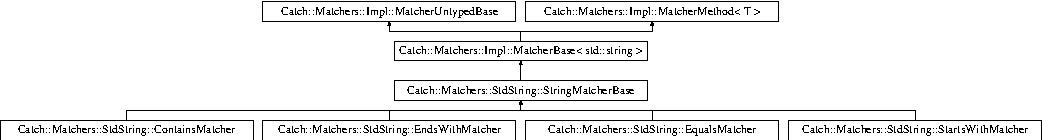
\includegraphics[height=1.879195cm]{struct_catch_1_1_matchers_1_1_std_string_1_1_string_matcher_base}
\end{center}
\end{figure}
\subsection*{Public Member Functions}
\begin{DoxyCompactItemize}
\item 
\mbox{\Hypertarget{struct_catch_1_1_matchers_1_1_std_string_1_1_string_matcher_base_a3a9b66bae298ae27058478529b4bb39d}\label{struct_catch_1_1_matchers_1_1_std_string_1_1_string_matcher_base_a3a9b66bae298ae27058478529b4bb39d}} 
{\bfseries String\+Matcher\+Base} (std\+::string const \&operation, \mbox{\hyperlink{struct_catch_1_1_matchers_1_1_std_string_1_1_cased_string}{Cased\+String}} const \&comparator)
\item 
\mbox{\Hypertarget{struct_catch_1_1_matchers_1_1_std_string_1_1_string_matcher_base_a47af030f8cea42a601ffb1000eea5cca}\label{struct_catch_1_1_matchers_1_1_std_string_1_1_string_matcher_base_a47af030f8cea42a601ffb1000eea5cca}} 
std\+::string {\bfseries describe} () const override
\end{DoxyCompactItemize}
\subsection*{Public Attributes}
\begin{DoxyCompactItemize}
\item 
\mbox{\Hypertarget{struct_catch_1_1_matchers_1_1_std_string_1_1_string_matcher_base_a17c9f0fe40587070ffe998c193742831}\label{struct_catch_1_1_matchers_1_1_std_string_1_1_string_matcher_base_a17c9f0fe40587070ffe998c193742831}} 
\mbox{\hyperlink{struct_catch_1_1_matchers_1_1_std_string_1_1_cased_string}{Cased\+String}} {\bfseries m\+\_\+comparator}
\item 
\mbox{\Hypertarget{struct_catch_1_1_matchers_1_1_std_string_1_1_string_matcher_base_a7a25c4b7d863e9a1c406d81efd0f83ca}\label{struct_catch_1_1_matchers_1_1_std_string_1_1_string_matcher_base_a7a25c4b7d863e9a1c406d81efd0f83ca}} 
std\+::string {\bfseries m\+\_\+operation}
\end{DoxyCompactItemize}
\subsection*{Additional Inherited Members}


The documentation for this struct was generated from the following file\+:\begin{DoxyCompactItemize}
\item 
catch.\+hpp\end{DoxyCompactItemize}

\hypertarget{class_catch_1_1_string_ref}{}\section{Catch\+:\+:String\+Ref Class Reference}
\label{class_catch_1_1_string_ref}\index{Catch\+::\+String\+Ref@{Catch\+::\+String\+Ref}}


{\ttfamily \#include $<$catch.\+hpp$>$}

\subsection*{Public Types}
\begin{DoxyCompactItemize}
\item 
\mbox{\Hypertarget{class_catch_1_1_string_ref_a06b4db8fc82b197004291cf370b2ba7c}\label{class_catch_1_1_string_ref_a06b4db8fc82b197004291cf370b2ba7c}} 
using {\bfseries size\+\_\+type} = std\+::size\+\_\+t
\end{DoxyCompactItemize}
\subsection*{Public Member Functions}
\begin{DoxyCompactItemize}
\item 
\mbox{\Hypertarget{class_catch_1_1_string_ref_a2f287267c3a988b288bfd910667c1cfc}\label{class_catch_1_1_string_ref_a2f287267c3a988b288bfd910667c1cfc}} 
{\bfseries String\+Ref} (\mbox{\hyperlink{class_catch_1_1_string_ref}{String\+Ref}} const \&other) noexcept
\item 
\mbox{\Hypertarget{class_catch_1_1_string_ref_a407d5737b94e5a374add5c2794589733}\label{class_catch_1_1_string_ref_a407d5737b94e5a374add5c2794589733}} 
{\bfseries String\+Ref} (\mbox{\hyperlink{class_catch_1_1_string_ref}{String\+Ref}} \&\&other) noexcept
\item 
\mbox{\Hypertarget{class_catch_1_1_string_ref_aea45f5089c53adac362bff6bd7c40943}\label{class_catch_1_1_string_ref_aea45f5089c53adac362bff6bd7c40943}} 
{\bfseries String\+Ref} (char const $\ast$raw\+Chars) noexcept
\item 
\mbox{\Hypertarget{class_catch_1_1_string_ref_a320bf235274ebb90dd6af80485af2797}\label{class_catch_1_1_string_ref_a320bf235274ebb90dd6af80485af2797}} 
{\bfseries String\+Ref} (char const $\ast$raw\+Chars, size\+\_\+type size) noexcept
\item 
\mbox{\Hypertarget{class_catch_1_1_string_ref_a7fe41469048f906e9a847798cd335f23}\label{class_catch_1_1_string_ref_a7fe41469048f906e9a847798cd335f23}} 
{\bfseries String\+Ref} (std\+::string const \&std\+String) noexcept
\item 
\mbox{\Hypertarget{class_catch_1_1_string_ref_a14d5a1983e33c51c6b5fd33bffbebabb}\label{class_catch_1_1_string_ref_a14d5a1983e33c51c6b5fd33bffbebabb}} 
auto {\bfseries operator=} (\mbox{\hyperlink{class_catch_1_1_string_ref}{String\+Ref}} const \&other) noexcept -\/$>$ \mbox{\hyperlink{class_catch_1_1_string_ref}{String\+Ref}} \&
\item 
\mbox{\Hypertarget{class_catch_1_1_string_ref_ad9fde21785affacc32d7da7a70d74e93}\label{class_catch_1_1_string_ref_ad9fde21785affacc32d7da7a70d74e93}} 
{\bfseries operator std\+::string} () const
\item 
\mbox{\Hypertarget{class_catch_1_1_string_ref_a8a843e39ad3560d10a80524ed926ed63}\label{class_catch_1_1_string_ref_a8a843e39ad3560d10a80524ed926ed63}} 
void {\bfseries swap} (\mbox{\hyperlink{class_catch_1_1_string_ref}{String\+Ref}} \&other) noexcept
\item 
\mbox{\Hypertarget{class_catch_1_1_string_ref_aabb30149ab961187e4b3ff3394bf6e73}\label{class_catch_1_1_string_ref_aabb30149ab961187e4b3ff3394bf6e73}} 
auto {\bfseries operator==} (\mbox{\hyperlink{class_catch_1_1_string_ref}{String\+Ref}} const \&other) const noexcept -\/$>$ bool
\item 
\mbox{\Hypertarget{class_catch_1_1_string_ref_aaa6c8bf61c4628034c19763d1c8ad215}\label{class_catch_1_1_string_ref_aaa6c8bf61c4628034c19763d1c8ad215}} 
auto {\bfseries operator!=} (\mbox{\hyperlink{class_catch_1_1_string_ref}{String\+Ref}} const \&other) const noexcept -\/$>$ bool
\item 
\mbox{\Hypertarget{class_catch_1_1_string_ref_a4ba2e01eec1f0f56c257d213c796ab3b}\label{class_catch_1_1_string_ref_a4ba2e01eec1f0f56c257d213c796ab3b}} 
auto {\bfseries operator\mbox{[}$\,$\mbox{]}} (size\+\_\+type index) const noexcept -\/$>$ char
\item 
\mbox{\Hypertarget{class_catch_1_1_string_ref_ac6b68b9dc1e1dec69e884e3f7be581bd}\label{class_catch_1_1_string_ref_ac6b68b9dc1e1dec69e884e3f7be581bd}} 
auto {\bfseries empty} () const noexcept -\/$>$ bool
\item 
\mbox{\Hypertarget{class_catch_1_1_string_ref_ae084d72cb2952cee61a63ef36611d0ad}\label{class_catch_1_1_string_ref_ae084d72cb2952cee61a63ef36611d0ad}} 
auto {\bfseries size} () const noexcept -\/$>$ size\+\_\+type
\item 
\mbox{\Hypertarget{class_catch_1_1_string_ref_a6a6cac7430e626ffdd7550a081e8168f}\label{class_catch_1_1_string_ref_a6a6cac7430e626ffdd7550a081e8168f}} 
auto {\bfseries number\+Of\+Characters} () const noexcept -\/$>$ size\+\_\+type
\item 
\mbox{\Hypertarget{class_catch_1_1_string_ref_a1669cb2765e820ca258159676cbd82a5}\label{class_catch_1_1_string_ref_a1669cb2765e820ca258159676cbd82a5}} 
auto {\bfseries c\+\_\+str} () const -\/$>$ char const $\ast$
\item 
\mbox{\Hypertarget{class_catch_1_1_string_ref_a248568b467cf6599320903ae613c8eee}\label{class_catch_1_1_string_ref_a248568b467cf6599320903ae613c8eee}} 
auto {\bfseries substr} (size\+\_\+type start, size\+\_\+type size) const noexcept -\/$>$ \mbox{\hyperlink{class_catch_1_1_string_ref}{String\+Ref}}
\item 
\mbox{\Hypertarget{class_catch_1_1_string_ref_aee240387305ca8b249169d79f36e7002}\label{class_catch_1_1_string_ref_aee240387305ca8b249169d79f36e7002}} 
auto {\bfseries current\+Data} () const noexcept -\/$>$ char const $\ast$
\end{DoxyCompactItemize}
\subsection*{Friends}
\begin{DoxyCompactItemize}
\item 
\mbox{\Hypertarget{class_catch_1_1_string_ref_a420e64e1652de1b0d427775781b018f5}\label{class_catch_1_1_string_ref_a420e64e1652de1b0d427775781b018f5}} 
struct {\bfseries String\+Ref\+Test\+Access}
\end{DoxyCompactItemize}


\subsection{Detailed Description}
A non-\/owning string class (similar to the forthcoming std\+::string\+\_\+view) Note that, because a \mbox{\hyperlink{class_catch_1_1_string_ref}{String\+Ref}} may be a substring of another string, it may not be null terminated. c\+\_\+str() must return a null terminated string, however, and so the \mbox{\hyperlink{class_catch_1_1_string_ref}{String\+Ref}} will internally take ownership (taking a copy), if necessary. In theory this ownership is not externally visible -\/ but it does mean (substring) String\+Refs should not be shared between threads. 

The documentation for this class was generated from the following file\+:\begin{DoxyCompactItemize}
\item 
catch.\+hpp\end{DoxyCompactItemize}

\hypertarget{class_space_test_1_1_test}{}\section{Space\+Test\+:\+:Test Class Reference}
\label{class_space_test_1_1_test}\index{Space\+Test\+::\+Test@{Space\+Test\+::\+Test}}
\subsection*{Static Public Member Functions}
\begin{DoxyCompactItemize}
\item 
\mbox{\Hypertarget{class_space_test_1_1_test_a5887b0a589deafcecd50c7c0018897d7}\label{class_space_test_1_1_test_a5887b0a589deafcecd50c7c0018897d7}} 
static bool {\bfseries t} (double a, double b)
\item 
\mbox{\Hypertarget{class_space_test_1_1_test_af846f71be01ca530273d23e3f6b3e9a2}\label{class_space_test_1_1_test_af846f71be01ca530273d23e3f6b3e9a2}} 
static bool {\bfseries t\+Int} (int a, int b)
\end{DoxyCompactItemize}


The documentation for this class was generated from the following file\+:\begin{DoxyCompactItemize}
\item 
Aron\+Lib.\+h\end{DoxyCompactItemize}

\hypertarget{class_catch_1_1_test_case}{}\section{Catch\+:\+:Test\+Case Class Reference}
\label{class_catch_1_1_test_case}\index{Catch\+::\+Test\+Case@{Catch\+::\+Test\+Case}}
Inheritance diagram for Catch\+:\+:Test\+Case\+:\begin{figure}[H]
\begin{center}
\leavevmode
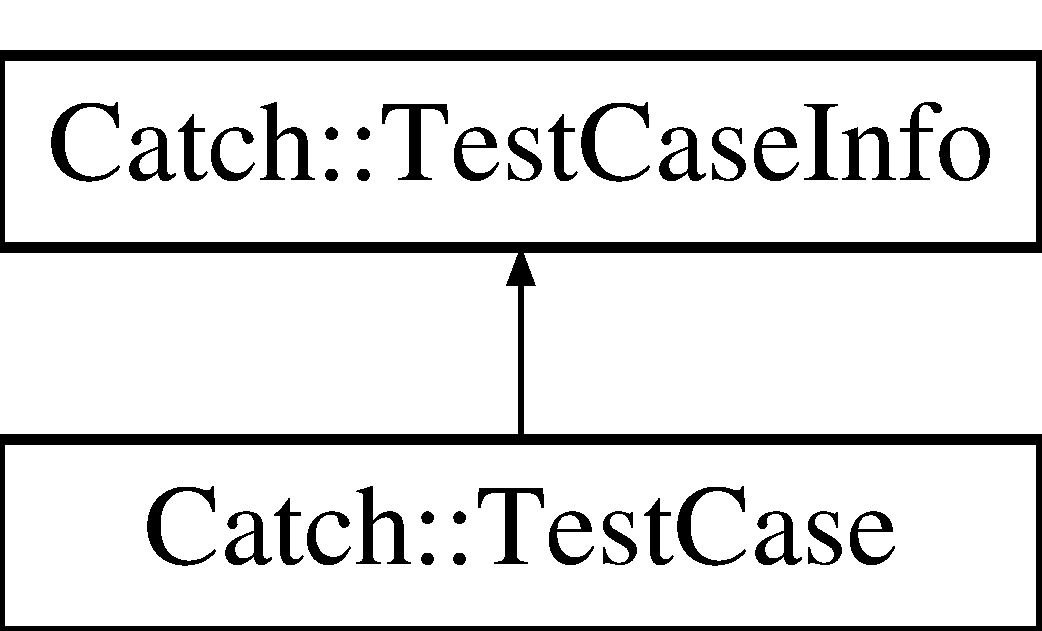
\includegraphics[height=2.000000cm]{class_catch_1_1_test_case}
\end{center}
\end{figure}
\subsection*{Public Member Functions}
\begin{DoxyCompactItemize}
\item 
\mbox{\Hypertarget{class_catch_1_1_test_case_aae5709fc1cb68e19ab0ac27e1ffd6a76}\label{class_catch_1_1_test_case_aae5709fc1cb68e19ab0ac27e1ffd6a76}} 
{\bfseries Test\+Case} (\mbox{\hyperlink{struct_catch_1_1_i_test_invoker}{I\+Test\+Invoker}} $\ast$test\+Case, \mbox{\hyperlink{struct_catch_1_1_test_case_info}{Test\+Case\+Info}} \&\&info)
\item 
\mbox{\Hypertarget{class_catch_1_1_test_case_a0812e8a216d09b087d5874687009f0d6}\label{class_catch_1_1_test_case_a0812e8a216d09b087d5874687009f0d6}} 
\mbox{\hyperlink{class_catch_1_1_test_case}{Test\+Case}} {\bfseries with\+Name} (std\+::string const \&\+\_\+new\+Name) const
\item 
\mbox{\Hypertarget{class_catch_1_1_test_case_a26f346c8446dded0562fe3818ae71651}\label{class_catch_1_1_test_case_a26f346c8446dded0562fe3818ae71651}} 
void {\bfseries invoke} () const
\item 
\mbox{\Hypertarget{class_catch_1_1_test_case_a1ea0d79f49156cebea076fe1ba50d2b6}\label{class_catch_1_1_test_case_a1ea0d79f49156cebea076fe1ba50d2b6}} 
\mbox{\hyperlink{struct_catch_1_1_test_case_info}{Test\+Case\+Info}} const  \& {\bfseries get\+Test\+Case\+Info} () const
\item 
\mbox{\Hypertarget{class_catch_1_1_test_case_a5456d03a90f75292835c158f3a3374a1}\label{class_catch_1_1_test_case_a5456d03a90f75292835c158f3a3374a1}} 
bool {\bfseries operator==} (\mbox{\hyperlink{class_catch_1_1_test_case}{Test\+Case}} const \&other) const
\item 
\mbox{\Hypertarget{class_catch_1_1_test_case_a030e4b9282e9b32e08c8bd5e5cd6fa98}\label{class_catch_1_1_test_case_a030e4b9282e9b32e08c8bd5e5cd6fa98}} 
bool {\bfseries operator$<$} (\mbox{\hyperlink{class_catch_1_1_test_case}{Test\+Case}} const \&other) const
\end{DoxyCompactItemize}
\subsection*{Additional Inherited Members}


The documentation for this class was generated from the following file\+:\begin{DoxyCompactItemize}
\item 
catch.\+hpp\end{DoxyCompactItemize}

\hypertarget{struct_catch_1_1_test_case_info}{}\section{Catch\+:\+:Test\+Case\+Info Struct Reference}
\label{struct_catch_1_1_test_case_info}\index{Catch\+::\+Test\+Case\+Info@{Catch\+::\+Test\+Case\+Info}}
Inheritance diagram for Catch\+:\+:Test\+Case\+Info\+:\begin{figure}[H]
\begin{center}
\leavevmode
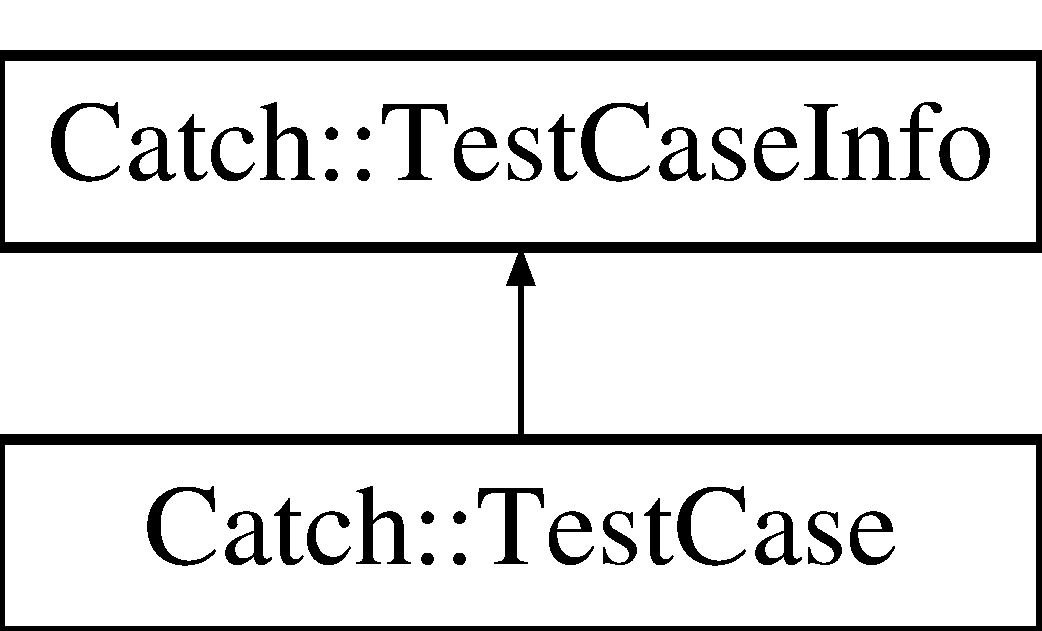
\includegraphics[height=2.000000cm]{struct_catch_1_1_test_case_info}
\end{center}
\end{figure}
\subsection*{Public Types}
\begin{DoxyCompactItemize}
\item 
\mbox{\Hypertarget{struct_catch_1_1_test_case_info_a39b232f74b4a7a6f2183b96759027eac}\label{struct_catch_1_1_test_case_info_a39b232f74b4a7a6f2183b96759027eac}} 
enum {\bfseries Special\+Properties} \{ \newline
{\bfseries None} = 0, 
{\bfseries Is\+Hidden} = 1 $<$$<$ 1, 
{\bfseries Should\+Fail} = 1 $<$$<$ 2, 
{\bfseries May\+Fail} = 1 $<$$<$ 3, 
\newline
{\bfseries Throws} = 1 $<$$<$ 4, 
{\bfseries Non\+Portable} = 1 $<$$<$ 5, 
{\bfseries Benchmark} = 1 $<$$<$ 6
 \}
\end{DoxyCompactItemize}
\subsection*{Public Member Functions}
\begin{DoxyCompactItemize}
\item 
\mbox{\Hypertarget{struct_catch_1_1_test_case_info_ad1a6b08b5a83d1c5eb4596b727b5305f}\label{struct_catch_1_1_test_case_info_ad1a6b08b5a83d1c5eb4596b727b5305f}} 
{\bfseries Test\+Case\+Info} (std\+::string const \&\+\_\+name, std\+::string const \&\+\_\+class\+Name, std\+::string const \&\+\_\+description, std\+::vector$<$ std\+::string $>$ const \&\+\_\+tags, \mbox{\hyperlink{struct_catch_1_1_source_line_info}{Source\+Line\+Info}} const \&\+\_\+line\+Info)
\item 
\mbox{\Hypertarget{struct_catch_1_1_test_case_info_a934b1a0952700743e99d62ec1731a2e2}\label{struct_catch_1_1_test_case_info_a934b1a0952700743e99d62ec1731a2e2}} 
bool {\bfseries is\+Hidden} () const
\item 
\mbox{\Hypertarget{struct_catch_1_1_test_case_info_afc70d4379a2070cc22b693ffe3932c1a}\label{struct_catch_1_1_test_case_info_afc70d4379a2070cc22b693ffe3932c1a}} 
bool {\bfseries throws} () const
\item 
\mbox{\Hypertarget{struct_catch_1_1_test_case_info_a5f37291295e3a6de2dd85324c941edaf}\label{struct_catch_1_1_test_case_info_a5f37291295e3a6de2dd85324c941edaf}} 
bool {\bfseries ok\+To\+Fail} () const
\item 
\mbox{\Hypertarget{struct_catch_1_1_test_case_info_abe33d81233230cdae8afa714688e905b}\label{struct_catch_1_1_test_case_info_abe33d81233230cdae8afa714688e905b}} 
bool {\bfseries expected\+To\+Fail} () const
\item 
\mbox{\Hypertarget{struct_catch_1_1_test_case_info_a17506de67fb18e27511c17f8a81119d8}\label{struct_catch_1_1_test_case_info_a17506de67fb18e27511c17f8a81119d8}} 
std\+::string {\bfseries tags\+As\+String} () const
\end{DoxyCompactItemize}
\subsection*{Public Attributes}
\begin{DoxyCompactItemize}
\item 
\mbox{\Hypertarget{struct_catch_1_1_test_case_info_a463794e2f5cfead307c93efd134ade36}\label{struct_catch_1_1_test_case_info_a463794e2f5cfead307c93efd134ade36}} 
std\+::string {\bfseries name}
\item 
\mbox{\Hypertarget{struct_catch_1_1_test_case_info_a1a5e0825132a38d091defdebbf2f8ce9}\label{struct_catch_1_1_test_case_info_a1a5e0825132a38d091defdebbf2f8ce9}} 
std\+::string {\bfseries class\+Name}
\item 
\mbox{\Hypertarget{struct_catch_1_1_test_case_info_a37fe2db9425bc45f6a33893eac31198e}\label{struct_catch_1_1_test_case_info_a37fe2db9425bc45f6a33893eac31198e}} 
std\+::string {\bfseries description}
\item 
\mbox{\Hypertarget{struct_catch_1_1_test_case_info_a150a7cbca1dd0c91799ccb14ff822eb0}\label{struct_catch_1_1_test_case_info_a150a7cbca1dd0c91799ccb14ff822eb0}} 
std\+::vector$<$ std\+::string $>$ {\bfseries tags}
\item 
\mbox{\Hypertarget{struct_catch_1_1_test_case_info_a844e3de9baf6e53cadfba9733c236bfe}\label{struct_catch_1_1_test_case_info_a844e3de9baf6e53cadfba9733c236bfe}} 
std\+::vector$<$ std\+::string $>$ {\bfseries lcase\+Tags}
\item 
\mbox{\Hypertarget{struct_catch_1_1_test_case_info_aa9407b7f442655b51a2aad24b3fa2fd3}\label{struct_catch_1_1_test_case_info_aa9407b7f442655b51a2aad24b3fa2fd3}} 
\mbox{\hyperlink{struct_catch_1_1_source_line_info}{Source\+Line\+Info}} {\bfseries line\+Info}
\item 
\mbox{\Hypertarget{struct_catch_1_1_test_case_info_afc1e84bd7a2e180895a06d9131302af0}\label{struct_catch_1_1_test_case_info_afc1e84bd7a2e180895a06d9131302af0}} 
Special\+Properties {\bfseries properties}
\end{DoxyCompactItemize}
\subsection*{Friends}
\begin{DoxyCompactItemize}
\item 
\mbox{\Hypertarget{struct_catch_1_1_test_case_info_a0fe44abaf18ae7c26f98a9fc2b08679c}\label{struct_catch_1_1_test_case_info_a0fe44abaf18ae7c26f98a9fc2b08679c}} 
void {\bfseries set\+Tags} (\mbox{\hyperlink{struct_catch_1_1_test_case_info}{Test\+Case\+Info}} \&test\+Case\+Info, std\+::vector$<$ std\+::string $>$ tags)
\end{DoxyCompactItemize}


The documentation for this struct was generated from the following file\+:\begin{DoxyCompactItemize}
\item 
catch.\+hpp\end{DoxyCompactItemize}

\hypertarget{struct_catch_1_1_test_failure_exception}{}\section{Catch\+:\+:Test\+Failure\+Exception Struct Reference}
\label{struct_catch_1_1_test_failure_exception}\index{Catch\+::\+Test\+Failure\+Exception@{Catch\+::\+Test\+Failure\+Exception}}


The documentation for this struct was generated from the following file\+:\begin{DoxyCompactItemize}
\item 
catch.\+hpp\end{DoxyCompactItemize}

\hypertarget{class_catch_1_1_test_invoker_as_method}{}\section{Catch\+:\+:Test\+Invoker\+As\+Method$<$ C $>$ Class Template Reference}
\label{class_catch_1_1_test_invoker_as_method}\index{Catch\+::\+Test\+Invoker\+As\+Method$<$ C $>$@{Catch\+::\+Test\+Invoker\+As\+Method$<$ C $>$}}
Inheritance diagram for Catch\+:\+:Test\+Invoker\+As\+Method$<$ C $>$\+:\begin{figure}[H]
\begin{center}
\leavevmode
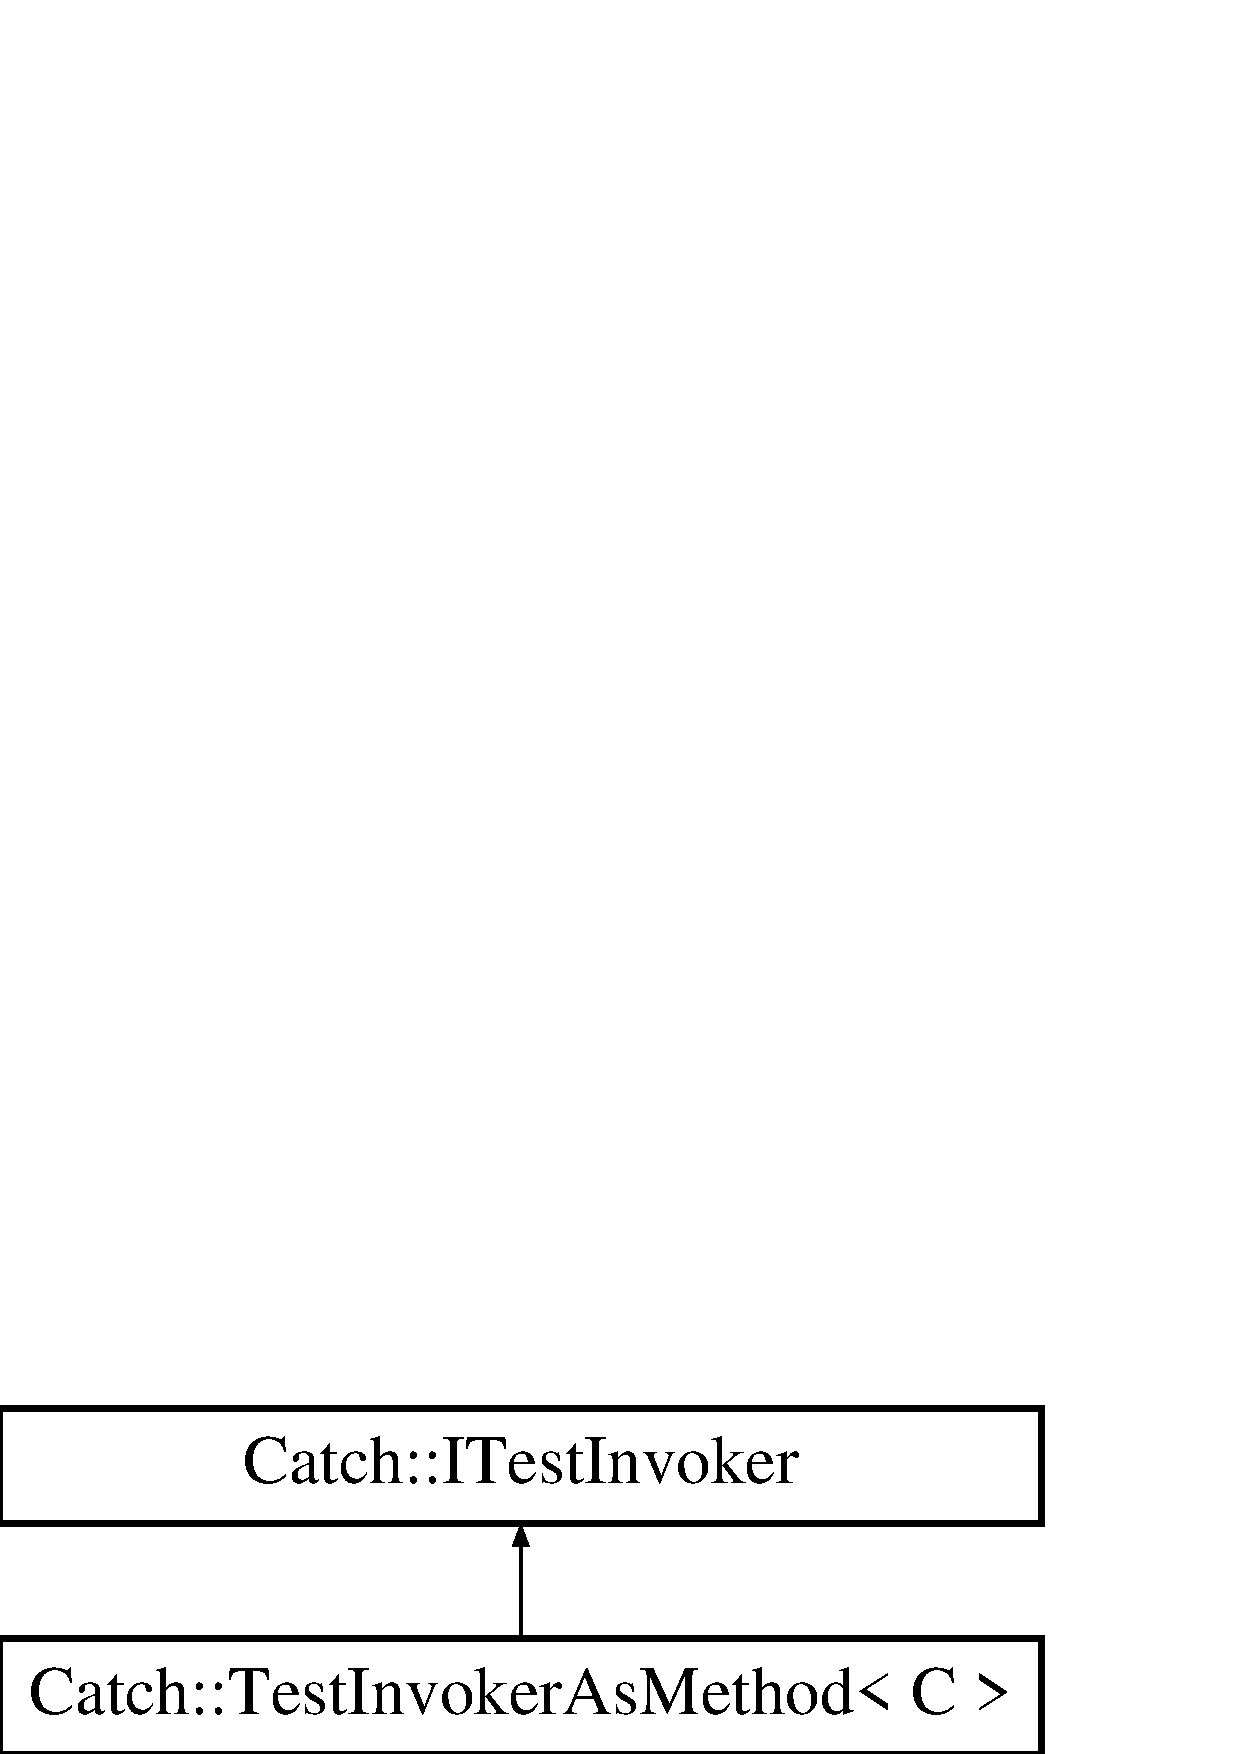
\includegraphics[height=2.000000cm]{class_catch_1_1_test_invoker_as_method}
\end{center}
\end{figure}
\subsection*{Public Member Functions}
\begin{DoxyCompactItemize}
\item 
\mbox{\Hypertarget{class_catch_1_1_test_invoker_as_method_a119c4bdbbdd95c42859c18541987a1a4}\label{class_catch_1_1_test_invoker_as_method_a119c4bdbbdd95c42859c18541987a1a4}} 
{\bfseries Test\+Invoker\+As\+Method} (void(C\+::$\ast$test\+As\+Method)()) noexcept
\item 
\mbox{\Hypertarget{class_catch_1_1_test_invoker_as_method_a8115a06efe273f4112ec0b5452c1b5f2}\label{class_catch_1_1_test_invoker_as_method_a8115a06efe273f4112ec0b5452c1b5f2}} 
void {\bfseries invoke} () const override
\end{DoxyCompactItemize}


The documentation for this class was generated from the following file\+:\begin{DoxyCompactItemize}
\item 
catch.\+hpp\end{DoxyCompactItemize}

\hypertarget{class_catch_1_1_timer}{}\section{Catch\+:\+:Timer Class Reference}
\label{class_catch_1_1_timer}\index{Catch\+::\+Timer@{Catch\+::\+Timer}}
\subsection*{Public Member Functions}
\begin{DoxyCompactItemize}
\item 
\mbox{\Hypertarget{class_catch_1_1_timer_a0a56e879e43f36c102bf9ea8b5fc8b72}\label{class_catch_1_1_timer_a0a56e879e43f36c102bf9ea8b5fc8b72}} 
void {\bfseries start} ()
\item 
\mbox{\Hypertarget{class_catch_1_1_timer_a57be5d17ca868a2d6fb1eea84de665cf}\label{class_catch_1_1_timer_a57be5d17ca868a2d6fb1eea84de665cf}} 
auto {\bfseries get\+Elapsed\+Nanoseconds} () const -\/$>$ uint64\+\_\+t
\item 
\mbox{\Hypertarget{class_catch_1_1_timer_a545de17a61a6fee1dbe3de5b0723e5fa}\label{class_catch_1_1_timer_a545de17a61a6fee1dbe3de5b0723e5fa}} 
auto {\bfseries get\+Elapsed\+Microseconds} () const -\/$>$ uint64\+\_\+t
\item 
\mbox{\Hypertarget{class_catch_1_1_timer_a30aaf458dbb59dd8ac8971c9c62e0eac}\label{class_catch_1_1_timer_a30aaf458dbb59dd8ac8971c9c62e0eac}} 
auto {\bfseries get\+Elapsed\+Milliseconds} () const -\/$>$ unsigned int
\item 
\mbox{\Hypertarget{class_catch_1_1_timer_a065e37e3c9eb16bd4dcf41971d8deedc}\label{class_catch_1_1_timer_a065e37e3c9eb16bd4dcf41971d8deedc}} 
auto {\bfseries get\+Elapsed\+Seconds} () const -\/$>$ double
\end{DoxyCompactItemize}


The documentation for this class was generated from the following file\+:\begin{DoxyCompactItemize}
\item 
catch.\+hpp\end{DoxyCompactItemize}

\hypertarget{class_torus}{}\section{Torus Class Reference}
\label{class_torus}\index{Torus@{Torus}}
\subsection*{Public Member Functions}
\begin{DoxyCompactItemize}
\item 
\mbox{\Hypertarget{class_torus_aef6376c3760a3a7226bd38392b0cb5d9}\label{class_torus_aef6376c3760a3a7226bd38392b0cb5d9}} 
{\bfseries Torus} (int numc, int numt)
\item 
\mbox{\Hypertarget{class_torus_aa2820070909448b22112cd6aa0bfc4bf}\label{class_torus_aa2820070909448b22112cd6aa0bfc4bf}} 
{\bfseries Torus} (int cx, int cy, int cz, int numc, int numt)
\item 
\mbox{\Hypertarget{class_torus_af86832d7a2bd688d2f491e5571235c4f}\label{class_torus_af86832d7a2bd688d2f491e5571235c4f}} 
void {\bfseries draw} ()
\end{DoxyCompactItemize}


The documentation for this class was generated from the following file\+:\begin{DoxyCompactItemize}
\item 
Torus.\+h\end{DoxyCompactItemize}

\hypertarget{struct_catch_1_1_totals}{}\section{Catch\+:\+:Totals Struct Reference}
\label{struct_catch_1_1_totals}\index{Catch\+::\+Totals@{Catch\+::\+Totals}}
\subsection*{Public Member Functions}
\begin{DoxyCompactItemize}
\item 
\mbox{\Hypertarget{struct_catch_1_1_totals_a9279ed39139cb7e7b291918a6d08290e}\label{struct_catch_1_1_totals_a9279ed39139cb7e7b291918a6d08290e}} 
\mbox{\hyperlink{struct_catch_1_1_totals}{Totals}} {\bfseries operator-\/} (\mbox{\hyperlink{struct_catch_1_1_totals}{Totals}} const \&other) const
\item 
\mbox{\Hypertarget{struct_catch_1_1_totals_a574015076e54cc405c70b053e3356e43}\label{struct_catch_1_1_totals_a574015076e54cc405c70b053e3356e43}} 
\mbox{\hyperlink{struct_catch_1_1_totals}{Totals}} \& {\bfseries operator+=} (\mbox{\hyperlink{struct_catch_1_1_totals}{Totals}} const \&other)
\item 
\mbox{\Hypertarget{struct_catch_1_1_totals_a1a94a654f5f3786b75695e081fc9bca2}\label{struct_catch_1_1_totals_a1a94a654f5f3786b75695e081fc9bca2}} 
\mbox{\hyperlink{struct_catch_1_1_totals}{Totals}} {\bfseries delta} (\mbox{\hyperlink{struct_catch_1_1_totals}{Totals}} const \&prev\+Totals) const
\end{DoxyCompactItemize}
\subsection*{Public Attributes}
\begin{DoxyCompactItemize}
\item 
\mbox{\Hypertarget{struct_catch_1_1_totals_a6ea14c7de7ea735a14f172a26e08a239}\label{struct_catch_1_1_totals_a6ea14c7de7ea735a14f172a26e08a239}} 
int {\bfseries error} = 0
\item 
\mbox{\Hypertarget{struct_catch_1_1_totals_a885ded66df752147b30c3d45aa602ec9}\label{struct_catch_1_1_totals_a885ded66df752147b30c3d45aa602ec9}} 
\mbox{\hyperlink{struct_catch_1_1_counts}{Counts}} {\bfseries assertions}
\item 
\mbox{\Hypertarget{struct_catch_1_1_totals_adb195fe477aedee2ecea88c888f16506}\label{struct_catch_1_1_totals_adb195fe477aedee2ecea88c888f16506}} 
\mbox{\hyperlink{struct_catch_1_1_counts}{Counts}} {\bfseries test\+Cases}
\end{DoxyCompactItemize}


The documentation for this struct was generated from the following file\+:\begin{DoxyCompactItemize}
\item 
catch.\+hpp\end{DoxyCompactItemize}

\hypertarget{class_catch_1_1_unary_expr}{}\section{Catch\+:\+:Unary\+Expr$<$ LhsT $>$ Class Template Reference}
\label{class_catch_1_1_unary_expr}\index{Catch\+::\+Unary\+Expr$<$ Lhs\+T $>$@{Catch\+::\+Unary\+Expr$<$ Lhs\+T $>$}}
Inheritance diagram for Catch\+:\+:Unary\+Expr$<$ LhsT $>$\+:\begin{figure}[H]
\begin{center}
\leavevmode
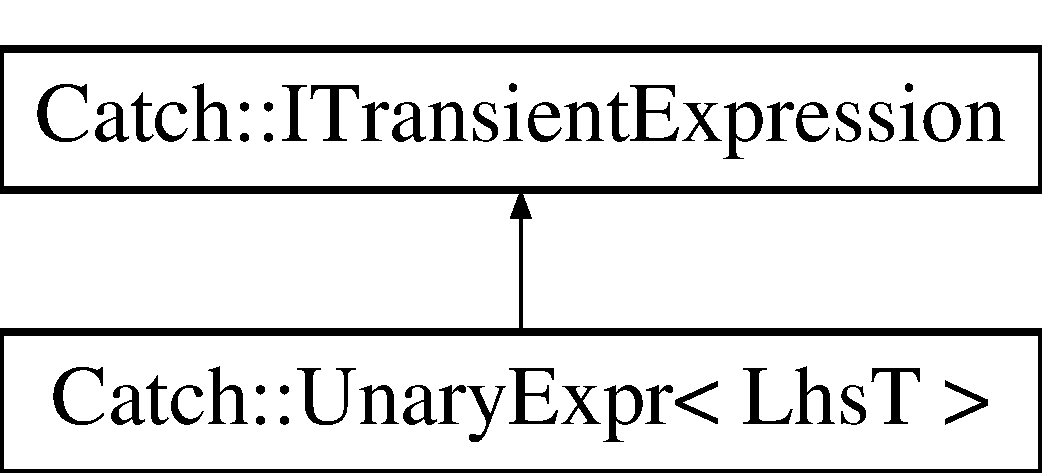
\includegraphics[height=2.000000cm]{class_catch_1_1_unary_expr}
\end{center}
\end{figure}
\subsection*{Public Member Functions}
\begin{DoxyCompactItemize}
\item 
\mbox{\Hypertarget{class_catch_1_1_unary_expr_ae02f666a1e64da728628aa2033e1d6e7}\label{class_catch_1_1_unary_expr_ae02f666a1e64da728628aa2033e1d6e7}} 
{\bfseries Unary\+Expr} (LhsT lhs)
\end{DoxyCompactItemize}
\subsection*{Additional Inherited Members}


The documentation for this class was generated from the following file\+:\begin{DoxyCompactItemize}
\item 
catch.\+hpp\end{DoxyCompactItemize}

\hypertarget{struct_catch_1_1_matchers_1_1_vector_1_1_unordered_equals_matcher}{}\section{Catch\+:\+:Matchers\+:\+:Vector\+:\+:Unordered\+Equals\+Matcher$<$ T $>$ Struct Template Reference}
\label{struct_catch_1_1_matchers_1_1_vector_1_1_unordered_equals_matcher}\index{Catch\+::\+Matchers\+::\+Vector\+::\+Unordered\+Equals\+Matcher$<$ T $>$@{Catch\+::\+Matchers\+::\+Vector\+::\+Unordered\+Equals\+Matcher$<$ T $>$}}
Inheritance diagram for Catch\+:\+:Matchers\+:\+:Vector\+:\+:Unordered\+Equals\+Matcher$<$ T $>$\+:\begin{figure}[H]
\begin{center}
\leavevmode
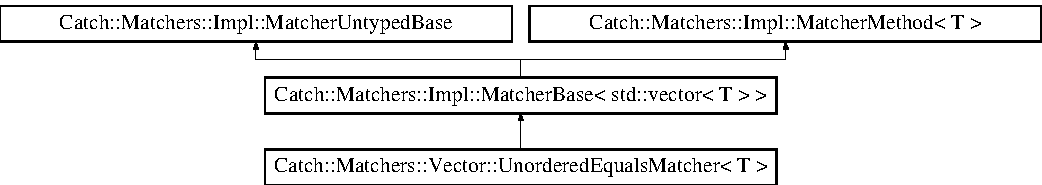
\includegraphics[height=2.492581cm]{struct_catch_1_1_matchers_1_1_vector_1_1_unordered_equals_matcher}
\end{center}
\end{figure}
\subsection*{Public Member Functions}
\begin{DoxyCompactItemize}
\item 
\mbox{\Hypertarget{struct_catch_1_1_matchers_1_1_vector_1_1_unordered_equals_matcher_a525905639b2b15b52ddb0bf14bfa19da}\label{struct_catch_1_1_matchers_1_1_vector_1_1_unordered_equals_matcher_a525905639b2b15b52ddb0bf14bfa19da}} 
{\bfseries Unordered\+Equals\+Matcher} (std\+::vector$<$ T $>$ const \&target)
\item 
\mbox{\Hypertarget{struct_catch_1_1_matchers_1_1_vector_1_1_unordered_equals_matcher_a3ccdd9dd2cd8bdbb8bb121acbb9cb358}\label{struct_catch_1_1_matchers_1_1_vector_1_1_unordered_equals_matcher_a3ccdd9dd2cd8bdbb8bb121acbb9cb358}} 
bool {\bfseries match} (std\+::vector$<$ T $>$ const \&vec) const override
\item 
\mbox{\Hypertarget{struct_catch_1_1_matchers_1_1_vector_1_1_unordered_equals_matcher_a7202d811200317abc58c844f663823df}\label{struct_catch_1_1_matchers_1_1_vector_1_1_unordered_equals_matcher_a7202d811200317abc58c844f663823df}} 
std\+::string {\bfseries describe} () const override
\end{DoxyCompactItemize}
\subsection*{Additional Inherited Members}


The documentation for this struct was generated from the following file\+:\begin{DoxyCompactItemize}
\item 
catch.\+hpp\end{DoxyCompactItemize}

\hypertarget{class_matrix_vector_1_1vec}{}\section{Matrix\+Vector\+:\+:vec Class Reference}
\label{class_matrix_vector_1_1vec}\index{Matrix\+Vector\+::vec@{Matrix\+Vector\+::vec}}
\subsection*{Public Member Functions}
\begin{DoxyCompactItemize}
\item 
\mbox{\Hypertarget{class_matrix_vector_1_1vec_ab6e2a9eafc93e30f80fa55c6c535d390}\label{class_matrix_vector_1_1vec_ab6e2a9eafc93e30f80fa55c6c535d390}} 
{\bfseries vec} (int r, int c)
\item 
\mbox{\Hypertarget{class_matrix_vector_1_1vec_a27d37d91d54816878e65731a1da0b356}\label{class_matrix_vector_1_1vec_a27d37d91d54816878e65731a1da0b356}} 
{\bfseries vec} (const \mbox{\hyperlink{class_matrix_vector_1_1vec}{vec}} \&v)
\item 
\mbox{\Hypertarget{class_matrix_vector_1_1vec_a3232c781891c2910d80415afacd6ea98}\label{class_matrix_vector_1_1vec_a3232c781891c2910d80415afacd6ea98}} 
\mbox{\hyperlink{class_matrix_vector_1_1vec}{vec}} {\bfseries operator+} (\mbox{\hyperlink{class_matrix_vector_1_1vec}{vec}} v)
\item 
\mbox{\Hypertarget{class_matrix_vector_1_1vec_a9803a34cc3d240ebf094f3769e9fabe9}\label{class_matrix_vector_1_1vec_a9803a34cc3d240ebf094f3769e9fabe9}} 
bool {\bfseries operator==} (const \mbox{\hyperlink{class_matrix_vector_1_1vec}{vec}} \&v)
\item 
\mbox{\Hypertarget{class_matrix_vector_1_1vec_ac9f996542c421f6c3914895ff01927a5}\label{class_matrix_vector_1_1vec_ac9f996542c421f6c3914895ff01927a5}} 
\mbox{\hyperlink{class_matrix_vector_1_1vec}{vec}} \& {\bfseries operator=} (const \mbox{\hyperlink{class_matrix_vector_1_1vec}{vec}} \&v)
\item 
\mbox{\Hypertarget{class_matrix_vector_1_1vec_a93520f50fed1ee242f2b2fb295565372}\label{class_matrix_vector_1_1vec_a93520f50fed1ee242f2b2fb295565372}} 
\mbox{\hyperlink{class_matrix_vector_1_1vec}{vec}} {\bfseries operator-\/} (\mbox{\hyperlink{class_matrix_vector_1_1vec}{vec}} \&v)
\item 
\mbox{\Hypertarget{class_matrix_vector_1_1vec_a48832bec7496fc407aad6130997ff829}\label{class_matrix_vector_1_1vec_a48832bec7496fc407aad6130997ff829}} 
\mbox{\hyperlink{class_matrix_vector_1_1mat}{mat}} {\bfseries operator$\ast$} (\mbox{\hyperlink{class_matrix_vector_1_1row}{row}} r)
\item 
\mbox{\Hypertarget{class_matrix_vector_1_1vec_a621b533b86d8986174e4b88c875a6c63}\label{class_matrix_vector_1_1vec_a621b533b86d8986174e4b88c875a6c63}} 
\mbox{\hyperlink{class_matrix_vector_1_1mat}{mat}} {\bfseries to\+Matrix} ()
\item 
\mbox{\Hypertarget{class_matrix_vector_1_1vec_a4602af813ed7eb84612e578aab0b91d0}\label{class_matrix_vector_1_1vec_a4602af813ed7eb84612e578aab0b91d0}} 
void {\bfseries print} ()
\item 
\mbox{\Hypertarget{class_matrix_vector_1_1vec_a2a2c95e44ec5fef8cbdcc8beca765b42}\label{class_matrix_vector_1_1vec_a2a2c95e44ec5fef8cbdcc8beca765b42}} 
\mbox{\hyperlink{class_matrix_vector_1_1row}{row}} {\bfseries tran} ()
\item 
\mbox{\Hypertarget{class_matrix_vector_1_1vec_a29697cf7bf95776710f673d6ea076d0f}\label{class_matrix_vector_1_1vec_a29697cf7bf95776710f673d6ea076d0f}} 
\mbox{\hyperlink{class_matrix_vector_1_1mat}{mat}} {\bfseries multi} ()
\item 
\mbox{\Hypertarget{class_matrix_vector_1_1vec_aaebd70c13be5311384dcf2bfdf4435fe}\label{class_matrix_vector_1_1vec_aaebd70c13be5311384dcf2bfdf4435fe}} 
void {\bfseries create\+Vec} (float $\ast$arr, int len)
\end{DoxyCompactItemize}
\subsection*{Public Attributes}
\begin{DoxyCompactItemize}
\item 
\mbox{\Hypertarget{class_matrix_vector_1_1vec_a9b2e20b78d4e28c76c5de2da43a9c952}\label{class_matrix_vector_1_1vec_a9b2e20b78d4e28c76c5de2da43a9c952}} 
int {\bfseries nrow}
\item 
\mbox{\Hypertarget{class_matrix_vector_1_1vec_aa0dc168f0f03f45db4aa9eee3234aa9c}\label{class_matrix_vector_1_1vec_aa0dc168f0f03f45db4aa9eee3234aa9c}} 
int {\bfseries ncol}
\item 
\mbox{\Hypertarget{class_matrix_vector_1_1vec_a5de4551d33631073af9e3fa31b13a508}\label{class_matrix_vector_1_1vec_a5de4551d33631073af9e3fa31b13a508}} 
float $\ast$$\ast$ {\bfseries arr}
\end{DoxyCompactItemize}


The documentation for this class was generated from the following file\+:\begin{DoxyCompactItemize}
\item 
Aron\+Lib.\+h\end{DoxyCompactItemize}

\hypertarget{class_aron_geometry_1_1_vector}{}\section{Aron\+Geometry\+:\+:Vector$<$ T $>$ Class Template Reference}
\label{class_aron_geometry_1_1_vector}\index{Aron\+Geometry\+::\+Vector$<$ T $>$@{Aron\+Geometry\+::\+Vector$<$ T $>$}}
\subsection*{Public Member Functions}
\begin{DoxyCompactItemize}
\item 
\mbox{\Hypertarget{class_aron_geometry_1_1_vector_ab0e5b0897f0b69f40394e210fa0fa7b1}\label{class_aron_geometry_1_1_vector_ab0e5b0897f0b69f40394e210fa0fa7b1}} 
{\bfseries Vector} (\mbox{\hyperlink{class_aron_geometry_1_1_point}{Point}}$<$ T $>$ p0, \mbox{\hyperlink{class_aron_geometry_1_1_point}{Point}}$<$ T $>$ p1)
\item 
\mbox{\Hypertarget{class_aron_geometry_1_1_vector_ac1e4622aaf8e4c4f043a0ddbb1c105e3}\label{class_aron_geometry_1_1_vector_ac1e4622aaf8e4c4f043a0ddbb1c105e3}} 
bool {\bfseries is\+Zero} ()
\item 
\mbox{\Hypertarget{class_aron_geometry_1_1_vector_a4f32e0511426c8430af6b7d871931540}\label{class_aron_geometry_1_1_vector_a4f32e0511426c8430af6b7d871931540}} 
\mbox{\hyperlink{class_aron_geometry_1_1_vector}{Vector}}$<$ T $>$ {\bfseries dir} ()
\item 
\mbox{\Hypertarget{class_aron_geometry_1_1_vector_adcca2e5f2b022cf628c894bf65667bae}\label{class_aron_geometry_1_1_vector_adcca2e5f2b022cf628c894bf65667bae}} 
\mbox{\hyperlink{class_aron_geometry_1_1_vector}{Vector}}$<$ T $>$ {\bfseries operator+} (\mbox{\hyperlink{class_aron_geometry_1_1_vector}{Vector}}$<$ T $>$ v)
\end{DoxyCompactItemize}
\subsection*{Public Attributes}
\begin{DoxyCompactItemize}
\item 
\mbox{\Hypertarget{class_aron_geometry_1_1_vector_a08859640da0f641d014f8985967f4fe4}\label{class_aron_geometry_1_1_vector_a08859640da0f641d014f8985967f4fe4}} 
\mbox{\hyperlink{class_aron_geometry_1_1_point}{Point}}$<$ T $>$ {\bfseries p0}
\item 
\mbox{\Hypertarget{class_aron_geometry_1_1_vector_a6f684e39725485dadce39a402b5ef248}\label{class_aron_geometry_1_1_vector_a6f684e39725485dadce39a402b5ef248}} 
\mbox{\hyperlink{class_aron_geometry_1_1_point}{Point}}$<$ T $>$ {\bfseries p1}
\end{DoxyCompactItemize}


The documentation for this class was generated from the following file\+:\begin{DoxyCompactItemize}
\item 
Aron\+Lib.\+h\end{DoxyCompactItemize}

\hypertarget{class_vector3}{}\section{Vector3 Class Reference}
\label{class_vector3}\index{Vector3@{Vector3}}
\subsection*{Public Member Functions}
\begin{DoxyCompactItemize}
\item 
\mbox{\Hypertarget{class_vector3_aad6b7d343e46f9d930139ebf3195a886}\label{class_vector3_aad6b7d343e46f9d930139ebf3195a886}} 
{\bfseries Vector3} (const \mbox{\hyperlink{class_vector3}{Vector3}} \&other)
\item 
\mbox{\Hypertarget{class_vector3_ad53e22b52babdb90d423601f72467590}\label{class_vector3_ad53e22b52babdb90d423601f72467590}} 
{\bfseries Vector3} (float x, float y, float z)
\item 
\mbox{\Hypertarget{class_vector3_a976712a6d78485facd87a07f689ffadf}\label{class_vector3_a976712a6d78485facd87a07f689ffadf}} 
{\bfseries Vector3} (float arr\mbox{[}3\mbox{]})
\item 
\mbox{\Hypertarget{class_vector3_a0edfaf32d40f9c40c694088fe2c46af7}\label{class_vector3_a0edfaf32d40f9c40c694088fe2c46af7}} 
\mbox{\hyperlink{class_vector3}{Vector3}} \& {\bfseries operator=} (const \mbox{\hyperlink{class_vector3}{Vector3}} \&rhs)
\item 
\mbox{\Hypertarget{class_vector3_ae29858b30586df4c855aa9be90bd8cd0}\label{class_vector3_ae29858b30586df4c855aa9be90bd8cd0}} 
\mbox{\hyperlink{class_vector3}{Vector3}} {\bfseries operator+} (\mbox{\hyperlink{class_vector3}{Vector3}} \&rhs)
\item 
\mbox{\Hypertarget{class_vector3_ab750fc3d6e61dbc6e724a1660d61c892}\label{class_vector3_ab750fc3d6e61dbc6e724a1660d61c892}} 
\mbox{\hyperlink{class_vector3}{Vector3}} {\bfseries operator-\/} (\mbox{\hyperlink{class_vector3}{Vector3}} \&rhs)
\item 
\mbox{\Hypertarget{class_vector3_ac0520d82b831dd7ec9e27b9ce802683c}\label{class_vector3_ac0520d82b831dd7ec9e27b9ce802683c}} 
\mbox{\hyperlink{class_vector3}{Vector3}} {\bfseries operator/} (float n)
\item 
\mbox{\Hypertarget{class_vector3_ac259eb9dd038c9c2bb67783e10e43748}\label{class_vector3_ac259eb9dd038c9c2bb67783e10e43748}} 
\mbox{\hyperlink{class_vector3}{Vector3}} {\bfseries dot} (\mbox{\hyperlink{class_vector3}{Vector3}} \&rhs)
\item 
\mbox{\Hypertarget{class_vector3_aa2d4b629b2d1260a49a88bd98c48934a}\label{class_vector3_aa2d4b629b2d1260a49a88bd98c48934a}} 
void {\bfseries print} ()
\end{DoxyCompactItemize}
\subsection*{Public Attributes}
\begin{DoxyCompactItemize}
\item 
\mbox{\Hypertarget{class_vector3_a0bac7304ad137502e0477b0a5ae716de}\label{class_vector3_a0bac7304ad137502e0477b0a5ae716de}} 
float {\bfseries v} \mbox{[}3\mbox{]}
\end{DoxyCompactItemize}


The documentation for this class was generated from the following file\+:\begin{DoxyCompactItemize}
\item 
Vector3.\+h\end{DoxyCompactItemize}

\hypertarget{class_space_vector4_1_1_vector4}{}\section{Space\+Vector4\+:\+:Vector4 Class Reference}
\label{class_space_vector4_1_1_vector4}\index{Space\+Vector4\+::\+Vector4@{Space\+Vector4\+::\+Vector4}}
\subsection*{Public Member Functions}
\begin{DoxyCompactItemize}
\item 
\mbox{\Hypertarget{class_space_vector4_1_1_vector4_a2d74027a6cd18790d44a35e07be057bc}\label{class_space_vector4_1_1_vector4_a2d74027a6cd18790d44a35e07be057bc}} 
{\bfseries Vector4} (const \mbox{\hyperlink{class_space_vector4_1_1_vector4}{Vector4}} \&other)
\item 
\mbox{\Hypertarget{class_space_vector4_1_1_vector4_af1defc2c881b55f3095b6d32024cf0cd}\label{class_space_vector4_1_1_vector4_af1defc2c881b55f3095b6d32024cf0cd}} 
{\bfseries Vector4} (float x, float y, float z, float w=1.\+0f)
\item 
\mbox{\Hypertarget{class_space_vector4_1_1_vector4_a9977965375a20112339df3b554312988}\label{class_space_vector4_1_1_vector4_a9977965375a20112339df3b554312988}} 
{\bfseries Vector4} (const float arr\mbox{[}4\mbox{]})
\item 
\mbox{\Hypertarget{class_space_vector4_1_1_vector4_a15181d0ac9fe25d8dac707c5cd4e44d6}\label{class_space_vector4_1_1_vector4_a15181d0ac9fe25d8dac707c5cd4e44d6}} 
{\bfseries Vector4} (float arr\mbox{[}4\mbox{]})
\item 
\mbox{\Hypertarget{class_space_vector4_1_1_vector4_a6724fb864b18b2d7e62327575deaa96d}\label{class_space_vector4_1_1_vector4_a6724fb864b18b2d7e62327575deaa96d}} 
bool {\bfseries operator==} (const \mbox{\hyperlink{class_space_vector4_1_1_vector4}{Vector4}} \&rhs)
\item 
\mbox{\Hypertarget{class_space_vector4_1_1_vector4_ac4f51027ef687a04d6aa10269fefda12}\label{class_space_vector4_1_1_vector4_ac4f51027ef687a04d6aa10269fefda12}} 
\mbox{\hyperlink{class_space_vector4_1_1_vector4}{Vector4}} \& {\bfseries operator=} (const \mbox{\hyperlink{class_space_vector4_1_1_vector4}{Vector4}} \&rhs)
\item 
\mbox{\Hypertarget{class_space_vector4_1_1_vector4_a9dccfd63d3647783c7736e61494bb88f}\label{class_space_vector4_1_1_vector4_a9dccfd63d3647783c7736e61494bb88f}} 
\mbox{\hyperlink{class_space_vector4_1_1_vector4}{Vector4}} {\bfseries operator+} (\mbox{\hyperlink{class_space_vector4_1_1_vector4}{Vector4}} \&rhs)
\item 
\mbox{\Hypertarget{class_space_vector4_1_1_vector4_ab42e4dc02ff63ecfb9610fb908268838}\label{class_space_vector4_1_1_vector4_ab42e4dc02ff63ecfb9610fb908268838}} 
\mbox{\hyperlink{class_space_vector4_1_1_vector4}{Vector4}} {\bfseries operator-\/} (\mbox{\hyperlink{class_space_vector4_1_1_vector4}{Vector4}} \&rhs)
\item 
\mbox{\Hypertarget{class_space_vector4_1_1_vector4_a903f6bb18d626e53572f7ba082da6af7}\label{class_space_vector4_1_1_vector4_a903f6bb18d626e53572f7ba082da6af7}} 
\mbox{\hyperlink{class_space_vector4_1_1_vector4}{Vector4}} {\bfseries operator/} (float n)
\item 
\mbox{\Hypertarget{class_space_vector4_1_1_vector4_ac9886e5653ff58bc53ad51269be4152c}\label{class_space_vector4_1_1_vector4_ac9886e5653ff58bc53ad51269be4152c}} 
float {\bfseries dot} (\mbox{\hyperlink{class_space_vector4_1_1_vector4}{Vector4}} \&rhs)
\item 
\mbox{\Hypertarget{class_space_vector4_1_1_vector4_ad4b3a6f298aea02980e96ede7862934a}\label{class_space_vector4_1_1_vector4_ad4b3a6f298aea02980e96ede7862934a}} 
float {\bfseries cross} (\mbox{\hyperlink{class_space_vector4_1_1_vector4}{Vector4}} \&rhs)
\item 
\mbox{\Hypertarget{class_space_vector4_1_1_vector4_af247a02d7575d01b94fb0d73ebc83230}\label{class_space_vector4_1_1_vector4_af247a02d7575d01b94fb0d73ebc83230}} 
\mbox{\hyperlink{class_space_vector4_1_1_vector4}{Vector4}} {\bfseries normal} ()
\item 
\mbox{\Hypertarget{class_space_vector4_1_1_vector4_aaaf481a5af47f864c00f444ca70acc1c}\label{class_space_vector4_1_1_vector4_aaaf481a5af47f864c00f444ca70acc1c}} 
const float \& {\bfseries operator\mbox{[}$\,$\mbox{]}} (int index) const
\item 
\mbox{\Hypertarget{class_space_vector4_1_1_vector4_aef75bb72cfd0532ef9310054884379b0}\label{class_space_vector4_1_1_vector4_aef75bb72cfd0532ef9310054884379b0}} 
float \& {\bfseries operator\mbox{[}$\,$\mbox{]}} (int index)
\item 
\mbox{\Hypertarget{class_space_vector4_1_1_vector4_a377cd13c9b345daea671af5ca02cd00d}\label{class_space_vector4_1_1_vector4_a377cd13c9b345daea671af5ca02cd00d}} 
void {\bfseries pp} ()
\item 
\mbox{\Hypertarget{class_space_vector4_1_1_vector4_adc32086423bc5abeeba57fb10bf81823}\label{class_space_vector4_1_1_vector4_adc32086423bc5abeeba57fb10bf81823}} 
void {\bfseries print} ()
\end{DoxyCompactItemize}
\subsection*{Public Attributes}
\begin{DoxyCompactItemize}
\item 
\mbox{\Hypertarget{class_space_vector4_1_1_vector4_a9bd51f001eb1a6b2435e613354351915}\label{class_space_vector4_1_1_vector4_a9bd51f001eb1a6b2435e613354351915}} 
const float {\bfseries e1} \mbox{[}4\mbox{]} = \{1.\+0f, 0.\+0f, 0.\+0f, 0.\+0f\}
\item 
\mbox{\Hypertarget{class_space_vector4_1_1_vector4_a7f87bb928e40319fb513f48ca5e9ee8a}\label{class_space_vector4_1_1_vector4_a7f87bb928e40319fb513f48ca5e9ee8a}} 
const float {\bfseries e2} \mbox{[}4\mbox{]} = \{0.\+0f, 1.\+0f, 0.\+0f, 0.\+0f\}
\item 
\mbox{\Hypertarget{class_space_vector4_1_1_vector4_a9845a51a0e1fa4994aadde9cb2957ff3}\label{class_space_vector4_1_1_vector4_a9845a51a0e1fa4994aadde9cb2957ff3}} 
const float {\bfseries e3} \mbox{[}4\mbox{]} = \{0.\+0f, 0.\+0f, 1.\+0f, 0.\+0f\}
\item 
\mbox{\Hypertarget{class_space_vector4_1_1_vector4_a1f753a69a011fbc593ec282769304ada}\label{class_space_vector4_1_1_vector4_a1f753a69a011fbc593ec282769304ada}} 
const float {\bfseries e4} \mbox{[}4\mbox{]} = \{0.\+0f, 0.\+0f, 0.\+0f, 1.\+0f\}
\end{DoxyCompactItemize}


The documentation for this class was generated from the following file\+:\begin{DoxyCompactItemize}
\item 
Aron\+Lib.\+h\end{DoxyCompactItemize}

\hypertarget{struct_catch_1_1_matchers_1_1_floating_1_1_within_abs_matcher}{}\section{Catch\+:\+:Matchers\+:\+:Floating\+:\+:Within\+Abs\+Matcher Struct Reference}
\label{struct_catch_1_1_matchers_1_1_floating_1_1_within_abs_matcher}\index{Catch\+::\+Matchers\+::\+Floating\+::\+Within\+Abs\+Matcher@{Catch\+::\+Matchers\+::\+Floating\+::\+Within\+Abs\+Matcher}}
Inheritance diagram for Catch\+:\+:Matchers\+:\+:Floating\+:\+:Within\+Abs\+Matcher\+:\begin{figure}[H]
\begin{center}
\leavevmode
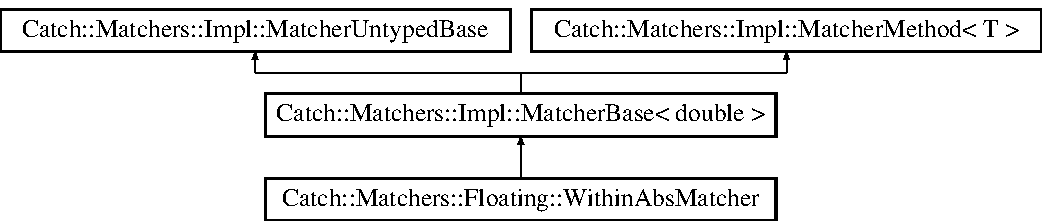
\includegraphics[height=2.968198cm]{struct_catch_1_1_matchers_1_1_floating_1_1_within_abs_matcher}
\end{center}
\end{figure}
\subsection*{Public Member Functions}
\begin{DoxyCompactItemize}
\item 
\mbox{\Hypertarget{struct_catch_1_1_matchers_1_1_floating_1_1_within_abs_matcher_ac45340b98c41230a7def5bd86c2d870f}\label{struct_catch_1_1_matchers_1_1_floating_1_1_within_abs_matcher_ac45340b98c41230a7def5bd86c2d870f}} 
{\bfseries Within\+Abs\+Matcher} (double target, double margin)
\item 
\mbox{\Hypertarget{struct_catch_1_1_matchers_1_1_floating_1_1_within_abs_matcher_afa5d8eed57f12c1e5d006471eb0bfe72}\label{struct_catch_1_1_matchers_1_1_floating_1_1_within_abs_matcher_afa5d8eed57f12c1e5d006471eb0bfe72}} 
bool {\bfseries match} (double const \&matchee) const override
\item 
\mbox{\Hypertarget{struct_catch_1_1_matchers_1_1_floating_1_1_within_abs_matcher_a206a738680f8767af31d3f1835afff3f}\label{struct_catch_1_1_matchers_1_1_floating_1_1_within_abs_matcher_a206a738680f8767af31d3f1835afff3f}} 
std\+::string {\bfseries describe} () const override
\end{DoxyCompactItemize}
\subsection*{Additional Inherited Members}


The documentation for this struct was generated from the following file\+:\begin{DoxyCompactItemize}
\item 
catch.\+hpp\end{DoxyCompactItemize}

\hypertarget{struct_catch_1_1_matchers_1_1_floating_1_1_within_ulps_matcher}{}\section{Catch\+:\+:Matchers\+:\+:Floating\+:\+:Within\+Ulps\+Matcher Struct Reference}
\label{struct_catch_1_1_matchers_1_1_floating_1_1_within_ulps_matcher}\index{Catch\+::\+Matchers\+::\+Floating\+::\+Within\+Ulps\+Matcher@{Catch\+::\+Matchers\+::\+Floating\+::\+Within\+Ulps\+Matcher}}
Inheritance diagram for Catch\+:\+:Matchers\+:\+:Floating\+:\+:Within\+Ulps\+Matcher\+:\begin{figure}[H]
\begin{center}
\leavevmode
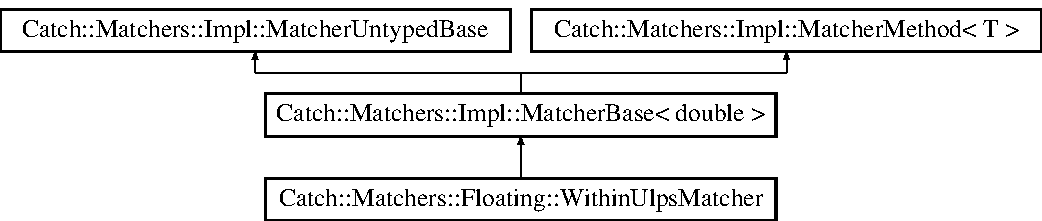
\includegraphics[height=2.968198cm]{struct_catch_1_1_matchers_1_1_floating_1_1_within_ulps_matcher}
\end{center}
\end{figure}
\subsection*{Public Member Functions}
\begin{DoxyCompactItemize}
\item 
\mbox{\Hypertarget{struct_catch_1_1_matchers_1_1_floating_1_1_within_ulps_matcher_a836074ae4010275284ab66b2485c6575}\label{struct_catch_1_1_matchers_1_1_floating_1_1_within_ulps_matcher_a836074ae4010275284ab66b2485c6575}} 
{\bfseries Within\+Ulps\+Matcher} (double target, int ulps, Floating\+Point\+Kind base\+Type)
\item 
\mbox{\Hypertarget{struct_catch_1_1_matchers_1_1_floating_1_1_within_ulps_matcher_aabda42a0dc5d00f3c5916feb75006b32}\label{struct_catch_1_1_matchers_1_1_floating_1_1_within_ulps_matcher_aabda42a0dc5d00f3c5916feb75006b32}} 
bool {\bfseries match} (double const \&matchee) const override
\item 
\mbox{\Hypertarget{struct_catch_1_1_matchers_1_1_floating_1_1_within_ulps_matcher_ad9bc8bb7f3abd326580a4bf6cf369b1b}\label{struct_catch_1_1_matchers_1_1_floating_1_1_within_ulps_matcher_ad9bc8bb7f3abd326580a4bf6cf369b1b}} 
std\+::string {\bfseries describe} () const override
\end{DoxyCompactItemize}
\subsection*{Additional Inherited Members}


The documentation for this struct was generated from the following file\+:\begin{DoxyCompactItemize}
\item 
catch.\+hpp\end{DoxyCompactItemize}

%--- End generated contents ---

% Index
\backmatter
\newpage
\phantomsection
\clearemptydoublepage
\addcontentsline{toc}{chapter}{Index}
\printindex

\end{document}
